\documentclass[leqno,b5paper]{book}
\usepackage{./tex/khalidUrduBooksEMT}                     %my sty file

%this file describes urdu commands for the commonly used english latex commands

%chapter, section etc
\newcommand*{\باب}[1]{\chapter{#1}}                                      %defining commonly used commands
\newcommand*{\حصہ}[1]{\section{#1}}
\newcommand*{\جزوحصہ}[1]{\subsection{#1}}
\newcommand*{\جزوجزوحصہ}[1]{\subsubsection{#1}}

\newcommand*{\بابء}[1]{\chapter*{#1}}                                      %defining commonly used commands
\newcommand*{\حصہء}[1]{\section*{#1}}
\newcommand*{\جزوحصہء}[1]{\subsection*{#1}}
\newcommand*{\جزوجزوحصہء}[1]{\subsubsection*{#1}}


%english text in urdu mode
\newcommand*{\تحریر}[1]{\textenglish{#1}}	% english text in urduMode
\newcommand*{\موٹا}[1]{\textbf{#1}}
\newcommand*{\ترچہ}[1]{{\textit{#1}}}
\newcommand*{\اصطلاح}[1]{{\textbf{#1}}}

%end commands cannot be redefined and as such these two are not usable
\providecommand*{\ابتدا}[1]{\begin{#1}}
\providecommand*{\انتہا}[1]{\end{#1}}

%include and input directives for adding external files into the main document 
\newcommand*{\بشمول}[1]{\includeonly{#1}}
\newcommand*{\شامل}[1]{\include{#1}}
\newcommand*{\داخل}[1]{\input{#1}}

%to use extra latex packages
\newcommand*{\استعمال}[1]{\usepackage{#1}}

%footnotes and indexes
\newcommand*{\حاشیہب}[1]{{\raggedright{\footnote{\textenglish{#1}}}} }               %footnote to the left hand side
\newcommand*{\حاشیہد}[1]{{\raggedleft{\footnote{#1}}}}
\newcommand*{\حاشیہط}[1]{\marginpar{#1}}

\newcommand*{\فرہنگ}[1]{\index{#1}}

%references and labels
\newcommand*{\شناخت}[1]{\label{#1}}
\newcommand*{\حوالہ}[1]{\ref{#1}}
\newcommand*{\حوالہصفحہ}[1]{\pageref{#1}}

%counters
\newcommand*{\فاصلہ}{\vspace*{10mm}}

%itemize, bullets and numbered items   
\newcommand*{\اشیاء}{itemize}                               %used in   \begin{itemize}
\newcommand*{\شے}[1]{\item {#1}}			%used in    \item

%maths commands
\newcommand*{\عددی}[1]{\: \ensuremath{#1} \:} % in-line math & inside math mode
\newcommand*{\عددیء}[1]{\ensuremath{#1}}
%\newcommand*{\سمتیہ}[1]{\ensuremath{\bf{#1}}}
\newcommand*{\سمتیہ}[1]{{\ensuremath{{\boldsymbol{#1}}}}}
\newcommand*{\سمتیہز}[2]{{\ensuremath{{\boldsymbol{#1}_{#2}}}}}     %with non-vector subscript
\newcommand*{\ضرب}{\time}					%multiplication symbol
\newcommand*{\نکطہد}{\cdot}
\newcommand*{\نقطے}{\ensuremath{\cdots}}

\newcommand*{\زیرنوشت}[3]{\: \ensuremath{{#1_{#2 \textrm {#3}}}} \:}   %english+urdu subscript \زیرنوشت{V}{CE}{غیرافزائندہ}
\newcommand*{\سیدھازیرنوشت}[2]{\: \ensuremath{{#1_{\textup{#2}}}} \:} %RC

\newcommand*{\قریب}[1]{\mbox{#1}}

\renewcommand{\indexname}{فرہنگ}        %apparently did nothing
%================================

%numbering scheme
\renewcommand*{\thefigure}{\arabic{figure}.\thechapter}
\renewcommand*{\thetable}{\arabic{table}.\thechapter}
\renewcommand*{\theequation}{\arabic{equation}.\thechapter}
\renewcommand*{\thesection}{\arabic{section}.\thechapter}
\renewcommand*{\thesubsection}{\arabic{subsection}.\arabic{section}.\thechapter}
\renewcommand*{\thesubsubsection}{\arabic{subsubsection}.\arabic{subsection}.\arabic{section}.\thechapter}

%================
%my environments
%================

%environment for examples مثال
\newcounter{examplecounter}[chapter]
\renewcommand{\theexamplecounter}{\arabic{examplecounter}.\thechapter}

\newenvironment*{مثال}
{\noindent\ignorespaces \vspace{\baselineskip} \hrule \vspace{\baselineskip}  مثال \refstepcounter{examplecounter} \theexamplecounter :}%
{\par\noindent \hrule  \vspace{\baselineskip}}

%------
%practice problems environment مشق

\newcounter{practicecounter}[chapter]                              %practice here means مشق
\renewcommand{\thepracticecounter}{\arabic{practicecounter}.\thechapter}

\newenvironment*{مشق}
{\noindent\ignorespaces \vspace{\baselineskip} \hrule \vspace{\baselineskip} مشق \refstepcounter{practicecounter} \thepracticecounter :}%
{\par\noindent \hrule  \vspace{\baselineskip}}
%---------

%end of chapter questions environment سوال

\newcounter{questioncounter}[chapter]
\renewcommand{\thequestioncounter}{\arabic{questioncounter}.\thechapter}

\newenvironment*{سوال}				
{\noindent\ignorespaces  سوال \refstepcounter{questioncounter} \thequestioncounter :}%
{\par\noindent }
                  %turning latex into urdu
% Greek Letters for Urdu Latex usage

\newcommand*{\ایلفا}{\alpha}
\newcommand*{\بیٹا}{\beta}
\newcommand*{\گیما}{\gamma}
\newcommand*{\ڈیلٹا}{\delta}
\newcommand*{\ایپسلان}{\epsilon}
\newcommand*{\متغیرایپسلان}{\varepsilon}
\newcommand*{\زیٹا}{\zeta}
\newcommand*{\ایٹا}{\eta}
\newcommand*{\تھیٹا}{\theta}
\newcommand*{\متغیرتھیٹا}{\vartheta}
\newcommand*{\ایوٹا}{\iota}
\newcommand*{\کاپا}{\kappa}
\newcommand*{\لیمڈا}{\lambda}
\newcommand*{\میو}{\mu}
\newcommand*{\نیو}{\nu}
\newcommand*{\ژاے}{\xi}
\newcommand*{\پاے}{\pi}
\newcommand*{\متغیرپاے}{\varpi}
\newcommand*{\رھو}{\rho}
\newcommand*{\متغیررھو}{\varrho}
\newcommand*{\سگما}{\sigma}
\newcommand*{\متغیرسگما}{\varsigma}
\newcommand*{\ٹو}{\tau}
\newcommand*{\اپسیلان}{\upsilon}
\newcommand*{\فاے}{\phi}
\newcommand*{\متغیفاے}{\varphi}
\newcommand*{\چاے}{\chi}
\newcommand*{\ساے}{\psi}
\newcommand*{\اومیگا}{\omega}

\newcommand*{\بڑاگیما}{\Gamma}
\newcommand*{\بڑاڈیلٹا}{\Delta}
\newcommand*{\بڑاتھیٹا}{\Theta}
\newcommand*{\بڑالیمڈا}{\Lambda}
\newcommand*{\بڑاژاے}{\Xi}
\newcommand*{\بڑاپاے}{\Pi}
\newcommand*{\بڑاسگما}{\Sigma}
\newcommand*{\بڑاساے}{\Psi}
\newcommand*{\بڑااومیگا}{\Omega}



\newcommand*{\kvec}[1]{{\ensuremath{{\boldsymbol{#1}}}}}
\newcommand*{\kvecsub}[2]{{\ensuremath{{\boldsymbol{#1}}}_{\textup{#2}}}}

\newcommand*{\ax}{\ensuremath{{\boldsymbol{a}}_{\textup{x}}}}
\newcommand*{\ay}{\ensuremath{{\boldsymbol{a}}_{\textup{y}}}}
\newcommand*{\az}{\ensuremath{{\boldsymbol{a}}_{\textup{z}}}}
%
\newcommand*{\arho}{\ensuremath{{\boldsymbol{a}}_{\rho}}}
\newcommand*{\aphi}{\ensuremath{{\boldsymbol{a}}_{\phi}}}
%
\newcommand*{\ar}{\ensuremath{{\boldsymbol{a}}_{\textup{r}}}}
\newcommand*{\atheta}{\ensuremath{{\boldsymbol{a}}_{\theta}}}

\newcommand*{\aN}{\ensuremath{{\boldsymbol{a}}_N}}

\newcommand*{\au}{\ensuremath{{\boldsymbol{a}}_u}}
\newcommand*{\av}{\ensuremath{{\boldsymbol{a}}_v}}
\newcommand*{\aw}{\ensuremath{{\boldsymbol{a}}_w}}

\newcommand*{\Ex}{\ensuremath{{\boldsymbol{E}}_x}}
\newcommand*{\Ey}{\ensuremath{{\boldsymbol{E}}_y}}
\newcommand*{\Ez}{\ensuremath{{\boldsymbol{E}}_z}}
%
\newcommand*{\Erho}{\ensuremath{{\boldsymbol{E}}_{\rho}}}
\newcommand*{\Ephi}{\ensuremath{{\boldsymbol{E}}_{\phi}}}
%
\newcommand*{\Er}{\ensuremath{{\boldsymbol{E}}_r}}
\newcommand*{\Etheta}{\ensuremath{{\boldsymbol{E}}_{\theta}}}

%%still decided to format everything at the very end
%try to make a jump table so that a single command can be built

\newcommand*{\ksubRB}{\ensuremath{R_{\textup{B}}}}   %transistor
\newcommand*{\ksubRC}{\ensuremath{R_{\textup{C}}}}
\newcommand*{\ksubRE}{\ensuremath{R_{\textup{E}}}}

\newcommand*{\ksubRG}{\ensuremath{R_{\textup{G}}}}	%mosfet
\newcommand*{\ksubRD}{\ensuremath{R_{\textup{D}}}}
\newcommand*{\ksubRS}{\ensuremath{R_{\textup{S}}}}

\newcommand*{\ksubCB}{\ensuremath{C_{\textup{B}}}}	%transistor
\newcommand*{\ksubCC}{\ensuremath{C_{\textup{C}}}}
\newcommand*{\ksubCE}{\ensuremath{C_{\textup{E}}}}

\newcommand*{\ksubCG}{\ensuremath{C_{\textup{G}}}}	%mosfet
\newcommand*{\ksubCD}{\ensuremath{C_{\textup{D}}}}
\newcommand*{\ksubCS}{\ensuremath{C_{\textup{S}}}}

\newcommand*{\ksubRCB}{\ensuremath{R_{\textup{CB}}}}    %resistor used with base capacitor    (GET RID OF SUCH USAGE)
\newcommand*{\ksubRCC}{\ensuremath{R_{\textup{CC}}}}   %resistor used with collector capacitor
\newcommand*{\ksubRCE}{\ensuremath{R_{\textup{CE}}}}   %resistor used with emitter capacitor

\newcommand*{\ksubVBE}{\ensuremath{V_{\textup{BE}}}}  %npnTransistor
\newcommand*{\ksubVBC}{\ensuremath{V_{\textup{BC}}}}
\newcommand*{\ksubVCE}{\ensuremath{V_{\textup{CE}}}}

\newcommand*{\ksubVEB}{\ensuremath{V_{\textup{EB}}}}  %pnpTransistor
\newcommand*{\ksubVCB}{\ensuremath{V_{\textup{CB}}}}
\newcommand*{\ksubVEC}{\ensuremath{V_{\textup{EC}}}}

\newcommand*{\ksubVGS}{\ensuremath{V_{\textup{GS}}}}  %nMosfet
\newcommand*{\ksubVGD}{\ensuremath{V_{\textup{GD}}}}
\newcommand*{\ksubVDS}{\ensuremath{V_{\textup{DS}}}}

\newcommand*{\ksubVSG}{\ensuremath{V_{\textup{SG}}}} 	%pMosfet
\newcommand*{\ksubVDG}{\ensuremath{V_{\textup{DG}}}}
\newcommand*{\ksubVSD}{\ensuremath{V_{\textup{SD}}}}

\newcommand*{\ksubsubVRE}{\ensuremath{V_{R_{\textup{E}}}}}
\newcommand*{\ksubsubVRC}{\ensuremath{V_{R_{\textup{C}}}}}
\newcommand*{\ksubsubVRB}{\ensuremath{V_{R_{\textup{B}}}}}

\newcommand*{\ksub}[2]{\ensuremath{#1_{\textup{#2}}}}     %R_1    or V_1   or C_1     where numbers are used

%voltage sources
\newcommand*{\ksubVCC}{\ensuremath{V_{\textup{CC}}}} %transistor
\newcommand*{\ksubVBB}{\ensuremath{V_{\textup{BB}}}}
\newcommand*{\ksubVEE}{\ensuremath{V_{\textup{EE}}}}

\newcommand*{\ksubVDD}{\ensuremath{V_{\textup{DD}}}}	%mosfet
\newcommand*{\ksubVGG}{\ensuremath{V_{\textup{GG}}}}
\newcommand*{\ksubVSS}{\ensuremath{V_{\textup{SS}}}}

\newcommand*{\ksubVS}{\ensuremath{V_{\textup{S}}}}
\newcommand*{\ksubVs}{\ensuremath{V_{\textup{s}}}}

%gain
\newcommand*{\ksubAv}{\ensuremath{A_{\textup{v}}}}		%gains
\newcommand*{\ksubAi}{\ensuremath{A_{\textup{i}}}}
\newcommand*{\ksubGm}{\ensuremath{G_{\textup{m}}}}
\newcommand*{\ksubRm}{\ensuremath{R_{\textup{m}}}}
         %these are all tested. to use at the very end when book is finished

\graphicspath{{./fig/figFrontPage/}{./fig/figBasicFacts/}{./fig/figMagneticCircuits/}{./fig/figTransformers/}{./fig/figEnergyConversion/}{./fig/figQuestions/}}		%paths to figures
%
%

%\includeonly{./tex/prefaceFirstBook,./tex/machBasicFacts,./tex/machMagneticCircuits,./tex/machTransformers,./tex/machElectroMechConv,./tex/machRotatingMachPrinciples,./tex/machSynchronous,./tex/machInduction,./tex/machDCmachines}
\includeonly{./tex/prefaceFirstBook,./tex/machElectroMechConv}
%\includeonly{./tex/emtSymbols,./tex/emtPreface,./tex/prefaceFirstBook,./tex/tikztest,./tex/k}



\author{
خالد خان یوسفزئی\\
{\small {کامسیٹ انسٹیٹیوٹ آف انفارمیشن ٹیکنالوجی، اسلام آباد}}\\
\texttt{khalidyousafzai@comsats.edu.pk}
}

\title{برقی آلات}
\date{}                           %if absent gives date in arabic which is a rubbish

\makeindex
%====================

\begin{document}
\begin{urdufont}

\renewcommand*{\contentsname}{عنوان}    %this command has to be placed right here

\frontmatter                          %just added instead of \pagenumbering{roman}
%%\pagenumbering{roman}    

\maketitle

\tableofcontents
\pagestyle{empty}
%\include{./tex/emtPreface}
\باب{دیباچہ}
گزشتہ چند برسوں سے حکومتِ پاکستان اعلیٰ تعلیم کی طرف توجہ دے رہی ہے جس سے ملک کی تاریخ میں پہلی مرتبہ اعلیٰ تعلیمی اداروں میں تحقیق کا رجحان پیدا ہوا ہے۔امید کی جاتی ہے کہ یہ سلسلہ جاری رہے گا۔

پاکستان میں اعلیٰ تعلیم کا نظام انگریزی زبان میں رائج ہے۔دنیا میں تحقیقی کام کا بیشتر حصہ انگریزی زبان میں ہی چھپتا ہے۔انگریزی زبان میں ہر موضوع پر لاتعداد کتابیں پائی جاتی ہیں جن سے طلبہ و طالبات استفادہ حاصل کر سکتے ہیں۔

ہمارے ملک میں طلبہ و طالبات کی ایک بہت بڑی تعداد بنیادی تعلیم اردو زبان میں حاصل کرتی ہے۔ان کے لئے انگریزی زبان میں موجود مواد سے استفادہ حاصل کرنا تو ایک طرف، انگریزی زبان ازخود ایک رکاوٹ کے طور پر ان کے سامنے آتی ہے۔یہ طلبہ و طالبات ذہین ہونے کے باوجود آگے بڑھنے اور قوم و ملک کی بھر پور خدمت کرنے کے قابل نہیں رہتے۔ایسے طلبہ و طالبات کو اردو زبان میں نصاب کی اچھی کتابیں درکار ہیں۔ہم نے قومی سطح پر ایسا کرنے کی کوئی خاطر خواہ کوشش نہیں کی۔ 

میں برسوں تک اس صورت حال کی وجہ سے پریشانی کا شکار رہا۔کچھ کرنے کی نیت رکھنے کے باوجود کچھ نہ کر سکتا تھا۔میرے لئے اردو میں ایک صفحہ بھی لکھنا ناممکن تھا۔آخر کار ایک دن میں نے اپنی اس کمزوری کو کتاب نہ لکھنے کا جواز بنانے سے انکار کر دیا اور یوں یہ کتاب وجود میں آئی۔

یہ کتاب اردو زبان میں تعلیم حاصل کرنے والے طلبہ و طالبات کے لئے نہایت آسان اردو میں لکھی گئی ہے۔کوشش کی گئی ہے کہ اسکول کی سطح پر نصاب میں استعمال تکنیکی الفاظ ہی استعمال کئے جائیں۔جہاں ایسے الفاظ موجود نہ تھے وہاں روز مرہ میں استعمال ہونے والے الفاظ چنے گئے۔تکنیکی الفاظ کی چنائی کے وقت اس بات کا دہان رکھا گیا کہ ان کا استعمال دیگر مضامین میں بھی ممکن ہو۔

کتاب میں بین الاقوامی نظامِ اکائی استعمال کی گئ ہے۔اہم متغیرات کی علامتیں وہی رکھی گئی ہیں جو موجودہ نظامِ تعلیم کی نصابی کتابوں میں رائج ہیں۔یوں اردو میں لکھی اس کتاب اور انگریزی میں اسی مضمون پر لکھی کتاب پڑھنے والے طلبہ و طالبات کو ساتھ کام کرنے میں دشواری نہیں ہو گی۔ 

امید کی جاتی ہے کہ یہ کتاب ایک دن خالصتاً اردو زبان میں انجنیئرنگ کی نصابی کتاب کے طور پر استعمال کی جائے گی۔اردو زبان میں الیکٹریکل انجنیئرنگ کی مکمل نصاب کی طرف یہ پہلا قدم ہے۔ 

اس کتاب کے پڑھنے والوں سے گزارش کی جاتی ہے کہ اسے زیادہ سے زیادہ طلبہ و طالبات تک پہنچانے میں مدد دیں اور انہیں جہاں اس کتاب میں غلطی نظر آئے وہ اس کی نشاندہی میری ای-میل پر کریں۔میں ان کا نہایت شکر گزار ہوں گا۔

اس کتاب میں تمام غلطیاں مجھ سے ہی ڈلی ہیں البتہ اسے درست بنانے میں بہت لوگوں کا ہاتھ ہے۔میں ان سب کا شکریہ ادا کرتا ہوں۔ یہ سلسلہ ابھی جاری ہے اور مکمل ہونے پر ان حضرات کے تاثرات یہاں شامل کئے جائیں گے۔  

میں یہاں کامسیٹ یونیورسٹی اور ہائر ایجوکیشن کمیشن کا شکریہ ادا کرنا چاہتا ہوں جن کی وجہ سے ایسی سرگرمیاں ممکن ہوئیں۔	
\vspace{5mm}

{\raggedleft{
خالد خان یوسفزئی

28 اکتوبر 2011}}

\include{./tex/emtSymbols}

\mainmatter                      %added this
%%\pagenumbering{arabic}   %instead of this

\pagestyle{headings}


%\باب{بنیادی حقائق}
اس کتاب میں جگہ جگہ مختلف حقائق آئیں گے جنہیں اس باب میں اکٹھے کرنے کی کوشش کی گئی ہے۔یہ توقع کی جاتی ہے کہ یوں کتاب پڑھتے وقت اصل مضمون پر توجہ رکھنا زیادہ آسان ہوگا۔

\حصہ{بنیادی اکائیاں}
اس کتاب میں  \اصطلاح{بین الاقوامی نظامِ اکائی}\حاشیہب{International System Of Units, SI} استعمال کیا جائے گا۔ اس نظام میں کمیت\حاشیہب{mass} کی اکائی \اصطلاح{کلوگرام}،  لمبائ کی اکائی \اصطلاح{میٹر} اور وقت کی اکائی \اصطلاح{سیکنڈ} ہے۔

\حصہ{مقداری}
وہ متغیرہ جس کی مقدار معین ہو اسے \اصطلاح{مقداری}\فرہنگ{مقداری}\حاشیہب{scalar}\فرہنگ{scalar} کہتے ہیں۔ اس کتاب میں مقداری متغیرہ کو سادہ طرز کی لکھائی میں انگریزی یا لاطینی زبان کے چھوٹے حروف  یعنی \عددی{a,b,\alpha,\cdots}  یا بڑے حروف یعنی  \عددی{A,B,\Psi,\cdots} سے ظاہر کیا جائے گا، مثلاً برقی رو کو \عددی{i} یا \عددی{I} سے ظاہر کیا جاتا ہے۔

\حصہ{سمتیہ}
	وہ خط جس کا طول اور سمت معین ہو، اسے \اصطلاح{سمتیہ}\فرہنگ{سمتیہ}\حاشیہب{vector}\فرہنگ{vector} کہتے ہیں۔ سمتیہ کو انگریزی یا لاطینی زبان کے چھوٹے یا  بڑے حروف،  جن کو موٹے طرز کی لکھائی میں لکھا گیا ہو،  سے ظاہر کیا جائے گا، مثلاً قوت کو \سمتیہ{F} سے ظاہر کیا جائے گا۔یہاں شکل \حوالہ{شکل_حقائق_اکائی_سمتیہ}  سے رجوع کرنا بہتر ہے۔ ایک ایسا سمتیہ جس کا طول ایک کے برابر ہو،  کو \اصطلاح{اکائی سمتیہ}\فرہنگ{اکائی سمتیہ}\حاشیہب{unit vector}\فرہنگ{unit vector} کہتے ہیں۔ اس کتاب میں اکائی سمتیہ کو انگریزی زبان کے پہلے حرف کو موٹے طرز کی لکھائ میں لکھا جائے گا، مثلاً اکائی سمتیہ \عددیء{\ax,\ay,\az} خلاء کی تین عمودی سمتوں کو ظاہر کرتے ہیں۔\عددیء{\ax} لکھتے ہوئے، زیرنوشت میں \عددیء{x}، اس بات کی نشان دہی  کرتا ہے کہ یہ اکائی سمتیہ خلاء کی \عددیء{x} سمت کو ظاہر کرتا ہے۔ اگر کسی سمتیہ  کا طول اور اس کی سمت کو علیحدہ علیحدہ لکھنا ہو تو اس کے طول کو ظاہر کرنے کے لئے سادہ طرز کی لکھائی میں وہی حرف استعمال کیا جائے گا جو اس سمتیہ کو ظاہر کرنے کے لئے، موٹے طرز کی لکھائی میں، استعمال کیا گیا ہو۔ یعنی سمتیہ \سمتیہ{F} کے طول کو \عددیء{F} سے ظاہر کیا جائے گا۔ شکل میں سمتیہ  \سمتیہ{F} کا طول \عددیء{F}، چار کے برابر ہے۔ اگر کسی سمتیہ کی سمت میں ایک اکائی سمتیہ بنایا جائے تو یہ اکائی سمتیہ اس سمتیہ کی سمت کو ظاہر کرتا ہے۔جیسے پہلے ذکر ہوا ہے  ایسے اکائی سمتیہ کو انگریزی کے پہلے حرف،  جس کو موٹے طرز کی لکھائی میں لکھا گیا ہو  سے ظاہر کیا جائے گا یعنی سمتیہ \سمتیہ{F} کی سمت کو \عددیء{\سمتیہ{a}_F} سے ظاہر کیا جائے گا۔یہاں،  زیرنوشت میں \عددیء{F} ، اس بات کی یاد دہانی کراتا ہے کہ یہ اکائی سمتیہ \سمتیہ{F} کی سمت کو ظاہر کر رہا ہے۔ شکل میں چونکہ قوت \سمتیہ{F} کا رخ دائیں جانب ہے لہٰذا  \عددیء{\سمتیہ{a}_F} اور  \عددیء{\ax} برابر ہیں۔
\begin{figure}
\centering
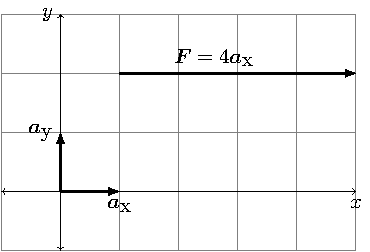
\includegraphics{figBasicFactsUnitVectors}
\caption{کارتیسی محدد}
\label{شکل_حقائق_اکائی_سمتیہ}
\end{figure}
%
\حصہ{محدد، خط مرتب}
ایک ایسا طریقہ جس کے ذریعہ کسی نقطہ کا مقام متعین کیا جا سکے کو خط مرتب یا محدد کہتے ہیں۔

	 خلاء تین طرفہ ہے۔ لہٰذا اس میں کسی ایک نقطہ کے مقام کو تین محدد کی مدد سے ظاہر کیا جا سکتا ہے۔ مزید یہ کہ خلاء میں کسی سمتیہ کو تین عمودی اکائی سمتیوں کی مدد سے لکھا جا سکتا ہے۔اب ہم ایسے چند محدد کے نظام دیکھتے ہیں۔

\جزوحصہ{کارتیسی محدد کا نظام}
	شکل \حوالہ{شکل_حقائق_اکائی_سمتیہ}   میں خلاء کی دو سمتیں اکائی سمتیہ \عددیء{\ax} اور \عددیء{\ay} سے ظاہر کی گئی ہیں۔یہ دونوں  آپس میں عمودی ہیں یعنی ان کا آپس میں \عددیء{90\degree}  کا زاویہ ہے۔خلاء تین طرفہ ہے لہٰذا اسے تین \اصطلاح{عمودی اکائی سمتیات}\فرہنگ{سمتیہ!عمودی اکائی}\حاشیہب{orthonormal vectors}\فرہنگ{orthonormal} سے ظاہر کیا جاتا ہے۔ ان سمتوں کی جانب،  طول  کو \عددیء{x,y,z} سے ظاہر کیا جاتا ہے۔ آپ ان سے بخوبی واقف ہیں۔ 


	 اگر دائیں ہاتھ کی چار انگلیوں کو \عددیء{\ax} کی جانب رکھ کر انہیں \عددیء{\ay} کی جانب موڑا جائے تو اس ہاتھ کا انگوٹھا \عددیء{\az} کی سمت کو ظاہر کرے گا۔لہٰذا،  خلاء کا  یہ  تین اکائی سمتوں والا نظام ایک \اصطلاح{دائیں ہاتھ کا نظام}\حاشیہب{right handed coordinate system}  ہے۔

	شکل \حوالہ{شکل_حقائق_کارتیسی_نظام_ایک_سمتیہ}  میں ایک سمتیہ \سمتیہ{A}، مرکز سے نقطہ \عددی{P(x,y,z)} تک بنایا گیا ہے۔اس سمتیہ کو ہم کارتیسی نظام محدد میں تین سمتیہ سے یوں ظاہر کر سکتے ہیں۔
\begin{align}
\kvec{A}=\kvec{A}_x+\kvec{A}_y+\kvec{A}_z
\end{align}
یا
\begin{align}
\kvec{A}=x\ax+y\ay+z\az
\end{align}
%
\begin{figure}
\centering
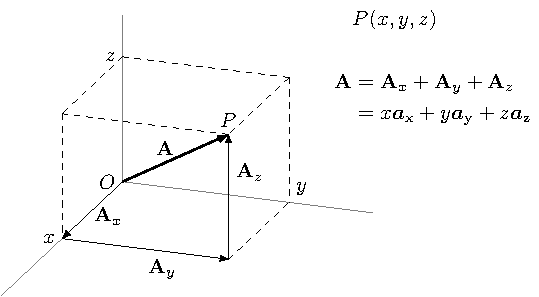
\includegraphics{figBasicFactsVectorCartesianCoordinates}
\caption{کارتیسی محدد نظام میں ایک سمتیہ}
\label{شکل_حقائق_کارتیسی_نظام_ایک_سمتیہ}
\end{figure}
%
کارتیسی محدد کے نظام میں اگر ہم متغیرہ \عددی{z} کو صفر رکھیں اور \عددیء{x,y} کو تبدیل کریں تو ہمیں  سطح \عددی{x-y} ملتی ہے۔ اس طرح اگر شکل \حوالہ{شکل_حقائق_کارتیسی_نظام_ایک_سمتیہ}  میں نقطہ \عددی{P(2,4,3)} ہو اور \عددیء{x-y} سطح کو زمین سمجھا جائے  تو شکل میں ڈبہ کے بالائی سطح پر  \عددی{z} کی مقدار معین ہے یعنی  \عددیء{z=3} جبکہ \عددی{x} صفر سے تین کے درمیان تبدیل اور \عددی{y} صفر سے چار کے درمیان تبدیل ہوتا ہے۔ یعنی اس ڈبہ کے بالائی سطح کو یوں لکھا جا سکتا ہے۔ 
\begin{align}
 \text{ڈبے کا بالائی سطح}= \left\{ 
  \begin{array}{l}
    0<x<2\\
    0<y<4 \\
	 z=3
  \end{array} \right.
\end{align}
اسی طرح اگر \عددیء{z} کو صفر اور تین کے درمیان ہر ممکن قیمت پر رکھ کر \عددی{x} اور \عددی{y} کو اسی طرح ان حدوں کے درمیان تبدیل کیا جائے تو ہمیں اس ڈبہ کا پورا حجم حاصل ہوگا۔ لہٰذا اس ڈبہ کے حجم کو ہم یوں لکھ سکتے ہیں۔
\begin{align}
 \text{ڈبے کاحجم}= \left\{ 
  \begin{array}{l}
    0<x<2\\
    0<y<4 \\
    0<z<3
  \end{array} \right.
\end{align}

\جزوحصہ{نلکی محدد کا نظام}
شکل \حوالہ{شکل_حقائق_نلکی_نظام_ایک_سمتیہ}  میں ایک سمتیہ  \سمتیہ{A} مرکز سے نقطہ \عددیء{P(x,y,z)} تک بنایا گیا ہے۔ اس سمتیہ کو شکل میں دو سمتیوں کی مدد سے ظاہر کیا گیا ہے۔ یعنی
\begin{align}
\kvec{A}=\kvec{\rho}+\kvec{A}_z
\end{align}
یا
\begin{align}
\kvec{A}=\rho \arho+z \az
\end{align}
%
\begin{figure}
\centering
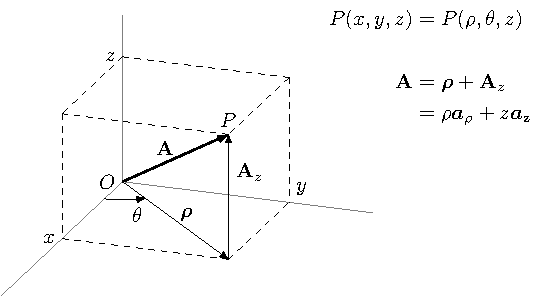
\includegraphics{figBasicFactsVectorCylindricalCoordinates}
\caption{نلکی محدد نظام}
\label{شکل_حقائق_نلکی_نظام_ایک_سمتیہ}
\end{figure}
سمتیہ $\arho$ سطح \عددی{x-y} پر ہے۔ اس شکل سے ظاہر ہے کہ
\begin{align}
x&=\rho \cos \theta\\
y&=\rho \sin \theta
\end{align}
لہٰذا ہم نقطہ \عددی{P(x,y,z)} کو متغیرہ \عددیء{x,y,z} کی جگہ متغیرہ \عددیء{\rho,\theta,z} کی مدد سے یوں لکھ سکتے ہیں \عددیء{P(\rho,\theta,z)}۔ لہٰذا ہم خلاء میں کسی بھی نقطہ کو اس کے تین متغیرہ \عددیء{\rho,\theta,z} سے ظاہر کر سکتے ہیں۔

	وہ نظام جس میں متغیرہ \عددیء{\rho,\theta,z}  کسی نقطہ کو متعین کرنے کے لئے استعمال ہو تو اس کو \اصطلاح{نلکی محدد}\فرہنگ{محدد!نلکی}\حاشیہب{cylindrical co-ordinates}\فرہنگ{cylindrical co-ordinates} کہتے ہیں۔یہاں شکل \حوالہ{شکل_حقائق_نلکی_نظام_تعریف}  سے رجوع کریں۔ اس نظام کے تین عمودی  اکائی سمتیہ $\arho,\atheta,\az$ ہیں۔ یہ نظام بھی دائیں ہاتھ کا نظام ہے۔ لہٰذا اگر دائیں ہاتھ کی چار انگلیوں کو اکائی سمتیہ $\arho$ کی جانب رکھ کر انہیں $\atheta$ کی جانب موڑیں تو اس ہاتھ کا انگوٹھا $\az$ کی سمت میں ہوگا۔ یہ تین عمودی اکائی سمتیہ کی تفصیل یوں ہے۔

سطح \عددی{x-y} میں مرکز پر، محدد \عددی{x} سے  زاویہ \عددی{\theta} کی  جانب اگر  اکائی سمتیہ بنائی جائے تو یہ اکائی سمتیہ $\arho$ ہو گی۔ اگر اسی سطح  \عددیء{x-y} پر اکائی سمتیہ $\arho$ کی عمودی سمت میں مرکز پر، زاویہ  \عددی{\theta} بڑھانے والے سمت میں، ایک اکائی سمتیہ بنائی جائے تو یہ  اکائی سمتیہ $\atheta$ ہو گی۔ اکائی سمتیہ $\az$ وہی اکائی سمتیہ ہے جو کارتیسی محدد نظام میں تھی۔ 
\begin{figure}
\centering
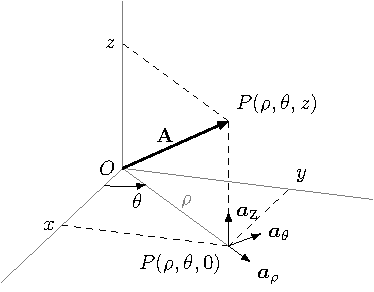
\includegraphics[height=3.5cm]{figBasicFactsCylindricalCoordinates}
\caption{نلکی نما محدد کی تعریف}
\label{شکل_حقائق_نلکی_نظام_تعریف}
\end{figure}
	یہاں یہ واضح رہے کہ اس نلکی محدد کے نظام  میں $\arho$ اور  $\atheta$ کی سمتیں ہر نقطہ پر مختلف ہیں جیسا کہ شکل \حوالہ{شکل_حقائق_نلکی_نظام_میں_اکائی_سمتیات_اٹل_نہیں} میں دکھایا گیا ہے۔

یہاں شکل \حوالہ{شکل_حقائق_نلکی_نظام_میں_دائرہ_اور_نلکی}  سے رجوع کریں۔ اگر نلکی محدد میں ایک سمتیہ ( جس کا متغیرہ \عددی{z} صفر کے برابر ہو، یعنی \عددی{z=0} ، اور اس کا رداس  \عددیء{\rho} ایک مستقل مقدار ہو مثلاً \عددیء{\rho=\rho_0}) کو یوں بنایا جائے کہ اس کا زاویہ \عددی{\theta} کو صفر سے  \عددیء{2 \pi} تک لے جایا جائے تو اس سمتیہ کی چونچ سطح \عددی{x-y} پر ایک دائرہ بنائے گی۔ اب اگر اسی سمتیہ کے متغیرہ \عددی{z} کو بھی تبدیل کیا جائے، مثلاً \عددی{z} کو صفر اور تین کے درمیان اس طرح تبدیل کیا جائے کہ ہر \عددی{\theta} پر \عددیء{z} کو صفر سے تین تک لے جایا جائے تو یہ سمتیہ ایک نلکی بنائے گی۔ اسی وجہ سے اس نظام کو نلکی محدد کہتے ہیں۔ اب اگر ہم سمتیہ کے تینوں متغیرہ تبدیل کریں تو ہمیں نلکی کا حجم ملتا ہے۔ اگلے تین مساوات ان باتوں کو ظاہر کرتے ہیں۔
\begin{align}
 \text{دائرہ}&= \left\{ 
  \begin{array}{l}
    \rho=\rho_0\\
    0<\theta<2 \pi \\
    z=0
  \end{array} \right.
\end{align}
%
\begin{align}
 \text{نلکی نما سطح}&= \left\{ 
  \begin{array}{l}
    \rho=\rho_0\\
    0<\theta<2 \pi \\
  0<z<z_0
  \end{array} \right.
\end{align}
%
\begin{align}
 \text{نلکی کا حجم}= \left\{ 
  \begin{array}{l}
    0<\rho<\rho_0\\
    0<\theta<2 \pi \\
  0<z<z_0
  \end{array} \right.
\end{align}
%
\begin{figure}
\centering
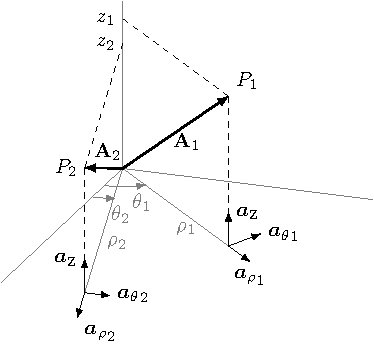
\includegraphics[height=3.5cm]{figBasicFactsCylindricalCoordinatesVaryingUnitVectors}
\caption{نلکی محدد میں اکائی سمتیہ \عددیء{\arho} اور \عددیء{\atheta} ہر نقطہ پر مختلف ہیں۔}
\label{شکل_حقائق_نلکی_نظام_میں_اکائی_سمتیات_اٹل_نہیں}
\end{figure}
%
\begin{figure}
\centering
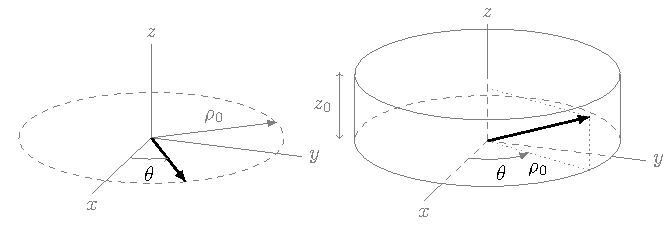
\includegraphics[height=2.5cm]{figBasicFactsCylindricalCoordinatesCircleAndCylinder}
\caption{‫نلکی محدد میں دائرہ اور نلکی‬}
\label{شکل_حقائق_نلکی_نظام_میں_دائرہ_اور_نلکی}
\end{figure}

\حصہ{سمتیہ رقبہ}
شکل \حوالہ{شکل_حقائق_رقبہ_سمتیہ} کو مدِ نظر رکھیں۔ کسی سطح سے اگر اس کے عمود کی جانب ایک فرضی لکیر کھینچی جائے تو اس  لکیر پر اکائی سمتیہ اس سطح کی سمت کو ظاہر کرتی ہے۔ چونکہ کسی بھی سطح، مثلاً اس کتاب کا ایک صفحہ،  کے دو اطراف ہوتے ہیں لہٰذا اس کے دو،  آپس میں اُلٹ،  سمتیں بیان کی جا سکتی ہیں۔عموما ً مسئلہ کو مدِ نظر رکھتے ہوئے  ان میں سے ایک سمت کو اس سطح کی سمت  لیا جاتا ہے۔ البتہ اگر یہ سطح بند سطح ہو ، مثلاً  گیند کی شکل کا ہو،  تب باہر جانب کو ہی اس سطح کی سمت لیا جاتا ہے۔ شکل میں اُوپر کی سطح \سمتیہ{A_1}  کا رقبہ \عددیء{A_1} ہے اور اس کی سمت $\az$ ہے۔ لہٰذا  \سمتیہ{A_1} سمتیہ کا طول  \عددیء{A_1} ہے اور اس کی سمت $\az$ ہے یعنی
\begin{figure}
\centering
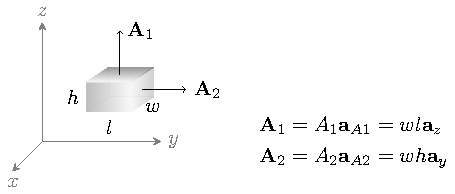
\includegraphics[height=2.5cm]{figBasicFactsVectorArea}
\caption{سمتیہ رقبہ کا تعارف‬}
\label{شکل_حقائق_رقبہ_سمتیہ}
\end{figure}
%
\begin{align*}
A_1&=wl\\
\kvec{a_{A1}}&=\az
\end{align*}
لہٰذا
\begin{align}
\kvec{A_1}=A_1 \kvec{a_{A1}}= w l \az
\end{align}
اسی طرح دائیں جانب سطح \سمتیہ{A_2} سمتیہ  کا طول \عددیء{A_2} ہے اور اس کی سمت \سمتیہ{a_{A2}} ہے۔ یعنی
\begin{align*}
A_2=wh\\
\kvec{a_{A2}}=\ay
\end{align*}
لہٰذا
\begin{align}
\kvec{A_2}=A_2 \kvec{a_{A1}}=w h \ay
\end{align}
یوں نیچے کی سطح کا رقبہ \عددیء{A_3=wl} ہے اور اس کی سمت خلاء کی  اکائی سمتیہ $\az$ کے اُلٹ ہے لہٰذا
\begin{align}
\kvec{A_3}=A_3 \kvec{a_{A3}}=wl (-\az)=-wl \az
\end{align}
یہاں دھیان کریں کہ رقبہ ہر صورت میں مثبت ہی ہوتا ہے البتہ اس کی سمت مثبت یا منفی ہو سکتی ہے۔ یہ بات کسی بھی سمتیہ کے لئے درست ہے لہٰذا کسی بھی سمتیہ کا طول ہر صورت میں مثبت ہی ہوتا ہے البتہ اس کی سمت مثبت یا منفی ہو سکتی ہے۔

\حصہ{رقبہ عمودی تراش}
زاویہ قائمہ بناتے ہوئے لمبائی میں کسی چیز کی کٹائی کو \اصطلاح{عمودی تراش}\فرہنگ{عمودی تراش}\حاشیہب{cross section}\فرہنگ{cross section} کہتے ہیں۔	

شکل \حوالہ{شکل_حقائق_رقبہ_عمودی}  میں ایک سلاخ دکھائی گئی ہے۔ اس کو اکائی سمتیہ $\ay$ کی سمت میں لٹایا گیا ہے۔ اگر ہم تصور میں اس سلاخ کو لمبائی کی عمودی سمت میں کاٹیں تو اس کا جو سرا بنے گا اس سطح کے رقبہ کو \اصطلاح{رقبہ عمودی تراش}\فرہنگ{عمودی تراش!رقبہ}\حاشیہب{cross sectional area} کہتے ہیں۔ شکل میں دکھایا گیا رقبہ عمودی تراش \سمتیہ{A} کی مقدار \عددیء{A} ہے جہاں
\begin{align}
A=wh
\end{align}
مسئلہ کو دیکھتے ہوئے اس رقبہ عمودی تراش کی سمت کا تعین کیا جاتا ہے۔ شکل میں اس کی سمت  \سمتیہ{a_A} خلاء کے اکائی سمتیہ  $\ay$ کی جانب ہے لہٰذا
\begin{align}
\kvec{a_A}=\ay
\end{align}
شکل میں بائیں جانب سلاخ کے نچلے کونے پر اکائی سمتیہ  $\ay$  اور  $\az$ دکھائے گئے ہیں۔ان کے ابتدائی نقطہ پر گول دائرہ میں ایک نقطہ دکھایا گیا ہے۔گول دائرہ میں بند نقطہ صفحہ سے عمودی طور پر کتاب کی باہر جانب سمت کو ظاہر کرتا ہے۔یہاں یہ سمتیہ  $\ax$ کی سمت دکھلا رہا ہے۔اس کی اُلٹ سمت یعنی صفحہ کی عمودی اندر کی جانب کو گول دائرہ میں بند صلیب کے نشان سے ظاہر کیا جاتا ہے۔
%
\begin{figure}
\centering
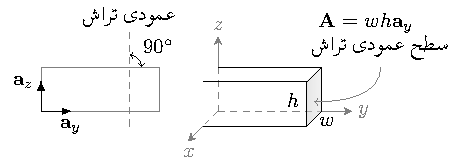
\includegraphics[height=2.5cm]{figBasicFactsCrossSectionalArea}
\caption{رقبہ  عمودی تراش}
\label{شکل_حقائق_رقبہ_عمودی}
\end{figure}
%
\حصہ{برقی میدان اور مقناطیسی میدان}
\جزوحصہ{برقی میدان اور برقی میدان کی شدت}
\اصطلاح{کولمب کے قانون}\فرہنگ{قانون!کولمب}\حاشیہب{Coulomb's law}\فرہنگ{Coulomb's law} کے تحت چارج شدہ جسموں کے درمیان قوت کشش\حاشیہب{attractive force} یا قوت دفع\حاشیہب{repulsive force} ان اجسام پر چارج کی مقدار کے حاصل ضرب کے راست متناسب اور باہمی فاصلہ کے مربع کے بالعکس متناسب ہوتی ہے۔ اس قانون کو مساوات کی شکل میں یوں لکھا جاتا ہے۔
\begin{align}
A=\frac{q_1 q_2}{4 \pi \epsilon r^2}
\end{align}
	اگر ایک چارج کسی جگہ موجود ہو اور دوسرا چارج اس کے قریب لایا جائے تو دوسرے چارج پر کشش یا دفع کی قوت عمل کرے گی جس کا تعین کولمب کے قانون سے ہوتا ہے۔ اگر دوسرے چارج کو پہلے چارج سے آہستہ آہستہ دور لے جائیں تو قوت کشش یا دفع کم ہوتی جاتی ہے۔ ایک خاص فاصلے کے بعد یہ قوت عملی طور پر صفر ہو جاتی ہے اور دوسرا چارج پہلے چارج کے حلقہ اثر سے باہر ہو جاتا ہے۔ اس حلقہ کے اندر واقع جگہ کو \اصطلاح{برقی میدان} کہا جاتا ہے۔ برقی میدان کسی ایک چارج کی وجہ سے بھی ہو سکتا ہے اور بہت سے چارجوں کی وجہ سے بھی ہو سکتا ہے۔ لہٰذا برقی میدان کی تعریف یوں کی جاتی ہے۔

 کسی چارج کے برقی میدان سے مراد چارج کے اِردگرد وہ جگہ ہے جس میں اس کا برقی اثر محسوس کیا جاتا ہے-

	\اصطلاح{برقی میدان کی شدت}\فرہنگ{برقی میدان!شدت}\حاشیہب{electric field intensity}\فرہنگ{electric field!intensity} \سمتیہ{E} کی مقدار اور اس کی سمت کسی مقام پر معلوم کرنے کا طریقہ یہ ہے کہ ایک مثبت اکائی چارج  کو اگر کسی چارج  \عددیء{Q} کے برقی میدان میں رکھا جائے تو جس سمت میں وہ مثبت اکائی چارج حرکت کرے یا حرکت کرنے کے لئے مائل ہو، وہی برقی میدان کی شدت کی سمت ہو گی اور جو قوت اس پر اثر انداز ہو وہ برقی میدان کی شدت ہوگی۔برقی میدان کی شدت کی اکائی \اصطلاح{وولٹ فی میٹر}\حاشیہب{\si{\volt / \meter}} ہے۔

	 کولمب کے قانون یعنی مساوات  کی مدد سے ایک چارج  \عددیء{Q} کی برقی میدان کی شدت کی مقدار یوں حاصل کی جا سکتی ہے۔چارج  \عددیء{Q} اور اکائی چارج یعنی ایک کولمب چارج کے درمیان قوتِ کشش یا قوتِ دفع 
\begin{align}
F=\frac{Q \times 1}{4 \pi \epsilon r^2}=\frac{Q}{4\pi\epsilon r^2}
\end{align}
نیوٹن ہو گی۔یہی برقی میدان کی شدت کی مقدار ہے یعنی
\begin{align}
E=\frac{Q}{4\pi\epsilon r^2}
\end{align}
اگر دو چارجوں کے درمیان سیدھی لکیر کھینچی جائے تو ان کے مابین قوتِ کشش یا قوتِ دفع کی سمت اس لکیر کی سمت میں ہو گی۔

\جزوحصہ{مقناطیسی میدان اور مقناطیسی میدان کی شدت}
\اصطلاح{مقناطیسی میدان} اور \اصطلاح{مقناطیسی میدان کی شدت}\فرہنگ{مقناطیسی میدان!شدت}\حاشیہب{magnetic field intensity}\فرہنگ{magnetic field!intensity} بالکل برقی میدان اور برقی میدان کی شدت کی طرح ہوتی ہے۔

	مقناطیسی میدان کی تعریف یوں کی جاتی ہے۔ کسی مقناطیس کے مقناطیسی میدان سے مراد مقناطیس کے اِردگرد وہ جگہ ہے جس میں اس کا مقناطیسی اثر محسوس کیا جاتا ہے۔

\حصہ{سطحی اور حجمی  کثافت}
\جزوحصہ{سطحی کثافت}
اکائی رقبہ کی سطح پر کسی چیز کی کُل مقدار کو اس چیز کی \اصطلاح{سطحی کثافت}\فرہنگ{سطحی کثافت}\حاشیہب{surface density}\فرہنگ{surface density} کہتے ہیں۔ مثال کے طور پر اگر رقبہ \عددیء{A} پر کسی متغیرہ کی کُل مقدار  \عددیء{\phi} ہو تب اس متغیرہ کی اوسط سطحی کثافت \سیدھازیرنوشت{B}{اوسط}  یہ ہوگی
\begin{align}
B_{\textup{اوسط}}=\frac{\phi}{A}
\end{align}
اس مساوات کو یوں بھی لکھا جا سکتا ہے
\begin{align}
\phi=B_{\textup{اوسط}} A
\end{align}
یعنی اگر ہمیں کسی سطح پر ایک متغیرہ کی اوسط سطحی کثافت معلوم ہو تب ہم اس سطح پر اس متغیرہ کی کُل مقدار اس مساوات کی مدد سے معلوم کر سکتے ہیں۔ 

اگر سطح پر متغیرہ ہر جگہ یکساں نہ ہو تب اس سطح پر سطحی کثافت جگہ جگہ تبدیل ہوگی۔ اس صورت میں اگر اتنا چھوٹا رقبہ لیا جائے کہ اس پر متغیرہ یکساں تصور کیا جا سکے تب اس نقطہ پر سطحی کثافت یوں حاصل ہوگی
\begin{align}
B=\frac{\Delta \phi}{\Delta A}
\end{align}
جہاں \عددیء{\Delta A} یہ چھوٹا رقبہ اور  \عددیء{\Delta \phi} اس پر متغیرہ کی چھوٹی سی مقدار ہے۔ اگر یہ رقبہ ایک نقطہ کی مانند کر دیا جائے تب اس مساوات کو یوں لکھا جائے گا۔
\begin{align}
B=\frac{\dif \phi}{\dif A}
\end{align}
 اس مساوات کو ہم یوں بھی بیان کر سکتے ہیں
\begin{align}
\dif \phi =B \dif A
\end{align}
یعنی اگر ہمیں کسی نقطہ پر ایک متغیرہ کی سطحی کثافت معلوم ہو تب اس نقطہ کے چھوٹے سے رقبہ پر ہم اس متغیرہ کی کم سے کم  کُل مقدار اس مساوات کی مدد سے معلوم کر سکتے ہیں۔

اسی طرح اگر ایک برقی تار کا رقبہ عمودی تراش \عددیء{A} ہو اور اس میں برقی رو \عددیء{I} گزر رہی ہو تو اس تار میں اوسط کثافتِ برقی رو 
\begin{align}
\rho_{\textup{اوسط}}=\frac{I}{A}
\end{align}
ہو گی۔

\حصہ{حجمی کثافت}
  اکائی حجم میں کسی چیز کی کُل مقدار کو اس چیز کی \اصطلاح{حجمی کثافت} کہتے ہیں۔یہاں ہم کمیت کی مثال لیتے ہیں۔ اگر کسی چیز کا حجم \عددیء{V} اور اس کی کمیت \عددیء{m} ہو تب اس کی اوسط حجمی کثافت یہ ہو گی۔
\begin{align}
\rho_{\textup{واسط}}=\frac{m}{V}
\end{align}
اسی طرح اگر اس چیز کی کمیت اس کے حجم میں جگہ جگہ مختلف ہو تب اس کی ایک نقطہ کی حجمی کثافت معلوم کرنے کے لئے اس کا اتنا چھوٹا حصہ لیا جاتا ہے کہ اس چھوٹے حصہ میں اس کی کمیت کو ہر جگہ یکساں تصور کیا جا سکے تب اس چھوٹے حصے کی حجمی کثافت یہ ہوگی۔
\begin{align}
\rho=\frac{\Delta m}{\Delta V}
\end{align}
اب اگر اس چھوٹے حصے کو ایک نقطہ مانند کر دیا جائے تب ہم لکھ سکتے ہیں کہ
\begin{align}
\rho=\frac{\dif m}{\dif V}
\end{align}
اور
\begin{align}
\dif m=\rho \dif V
\end{align}
یعنی اگر ہمیں ایک نقطہ کی حجمی کثافت معلوم ہو تب ہم ایک نہایت چھوٹے حجم کی کمیت اس مساوات کی مدد سے حاصل کر سکتے ہیں۔

\حصہ{ضربِ صلیبی اور ضربِ نقطہ}
دو مقداری متغیرات کا حاصلِ ضرب مقداری متغیرہ ہی ہوتی ہے جبکہ دو سمتیہ متغیرات کا حاصلِ ضرب سمتیہ متغیرہ یا مقداری متغیرہ ہو سکتی ہے۔ان دو اقسام کے ضرب پر یہاں غور کیا جائے گا۔
\جزوحصہ{ضرب صلیبی}
ایسی دو سمتیہ متغیرات کا ضرب جس کا حاصلِ ضرب سمتیہ متغیرہ ہو کو ضربِ صلیبی کہتے ہیں اور اسے یوں لکھا جاتا ہے۔
\begin{align}
\kvec{C}=\kvec{A} \times \kvec{B}
\end{align}
ضربِ صلیبی میں ضرب کے نشان کو صلیب کی علامت سے ظاہر کیا جاتا ہے۔اسی سے اس کا نام ضربِ صلیبی لیا گیا ہے۔

حاصل ضرب سمتیہ \سمتیہ{C} کی مقدار
\begin{gather}
\begin{aligned}
C=\abs{\kvec{C}} &= \abs {\kvec{A}} \abs{\kvec{B}} \sin \theta_{AB}\\
&=A B \sin \theta_{AB}
\end{aligned}
\end{gather}
ہے جہاں \عددیء{\theta_{AB}} ان کے مابین زاویہ ہے۔اس حاصل سمتیہ کی سمت دائیں ہاتھ  کے قانون سے یوں حاصل کی جاتی ہے۔ 

اگر آپ دائیں ہاتھ کی چار انگلیوں کو سمتیہ \سمتیہ{A} کی سمت میں رکھ کر \سمتیہ{B} سمتیہ کی سمت موڑیں تو اس ہاتھ کا انگوٹھا \سمتیہ{C}  سمتیہ کی سمت کو ظاہر کرے گا۔

\ابتدا{مثال}
مندرجہ ذیل ضرب صلیبی حاصل کریں۔
\begin{itemize}
\item
$\ax \times \ay \quad \ay \times \az \quad \az \times \ax \quad \ax \times \az$ \\
\item
 $\az \times \ay \quad \ay \times \ay \quad \arho \times \atheta \quad \az \times \arho$
\end{itemize}

حل: اس مثال میں سب سمتیہ اکائی ہیں۔اکائی سمتیہ کا طول ایک کے برابر ہوتا ہے۔ لہٰذا
\begin{itemize}
\item
$\ax \times \ay=(1)(1) \sin 90 \az =\az$\\
\item
$\ay \times \az=(1)(1) \sin 90 \ax =\ax$\\
\item
$\az \times \ax=(1)(1) \sin 90 \ay =\ay$\\
\item
$\ax \times \az=(1)(1) \sin 90 (-\ay) =-\ay$\\
\item
$\az \times \ay=(1)(1) \sin 90 (-\ax) =-\ax$\\
\item
اس مثال میں چونکہ دونوں سمتیہ ایک ہی جانب ہیں لہٰذا ان کے مابین زاویہ صفر ہے۔صفر زاویہ کا سائن صفر ہی ہوتا ہے یعنی \عددیء{\sin 0 =0} لہٰذا ان دو سمتیہ کا ضربِ صلیبی صفر ہو گا\\
$\ay \times \ay=(1)(1) \sin 0  =0$\\
\item
$\arho \times \atheta=(1)(1) \sin 90  \az =\az$\\
\item
$\az \times \arho=(1)(1) \sin 90 \atheta =\atheta $\\
\end{itemize}
\انتہا{مثال}
%
\ابتدا{مثال}
شکل \حوالہ{شکل_حقائق_کارتیسی_مروڑ_کا_حل} میں  چار نیوٹن کی قوت \سمتیہ{F} محور سے تین میٹر کی سمتیہ فاصلہ \سمتیہ{L}  پر لاگو ہے۔اسی شکل میں اس کی تفصیل دی گئی ہے۔اس قوت کی مروڑ  حاصل کریں۔
	حل:
	مروڑ \سمتیہ{T} کی تعریف یہ ہے
\begin{align}
\kvec{T}=\kvec{L} \times \kvec{F}
\end{align}
کارتیسی نظام میں اس سمتیہ فاصلہ کو یوں لکھا جا سکتا ہے
\begin{align}
\kvec{L}=L \sin \theta \ax-L \cos \theta \ay
\end{align}
لہٰذا
\begin{align*}
\kvec{T}&=\left(L \sin \theta \ax-L \cos \theta \ay \right) \times F \ay\\
&=L \sin \theta \ax \times F \ay-L \cos \theta \ay \times F \ay\\
&= L F \sin \theta \az
\end{align*} 
یہاں پچھلی مثال کی مدد سے \عددیء{\ax \times \ay=\az} اور \عددیء{\ay \times \ay=0} لی گئی ہیں۔یوں
\begin{align*}
\kvec{T}= L F \sin \theta \az=12 \sin \theta \az \quad \si{\newton \meter}
\end{align*}
ہے۔اس مثال میں \عددیء{\theta_{LF}=180\degree-\theta} ہے۔چونکہ کسی بھی زاویہ \عددیء{\alpha}   کے لئے \عددیء{\sin \alpha=\sin(180\degree-\alpha)} ہوتا ہے لہٰذا اس مروڑ کو یوں بھی لکھا جا سکتا ہے۔
\begin{align*}
\kvec{T}&=LF\sin \theta \az\\
&=L F \sin \theta_{LF}\az
\end{align*}
یہی جواب ضربِ صلیبی کی تعریف یعنی مساوات اور دائیں ہاتھ کے قانون کی مدد سے زیادہ آسانی سے حاصل ہوتا ہے۔
\انتہا{مثال}
%
\begin{figure}
\centering
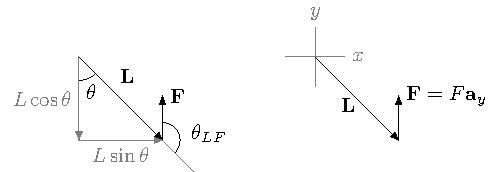
\includegraphics[height=2.5cm]{figBasicFactsVectorCrossProduct}
\caption{کارتیسی نظام میں مروڑ کا حل}
\label{شکل_حقائق_کارتیسی_مروڑ_کا_حل}
\end{figure}
%
\جزوحصہ{ضربِ نقطہ}
ایسی دو سمتیہ متغیرات کا ضرب جس کا حاصلِ ضرب مقداری متغیرہ ہو کو ضربِ نقطہ کہتے ہیں اور اسے یوں لکھا جاتا ہے۔
\begin{align}
\kvec{C}=\kvec{A} \cdot \kvec{B}
\end{align}
ضربِ نقطہ میں ضرب کے نشان کو نقطہ کی علامت سے ظاہر کیا جاتا ہے۔اسی سے اس کا نام ضربِ نقطہ لیا گیا ہے۔

ضربِ نقطہ میں حاصلِ ضرب مقداری کی مقدار یوں حاصل ہوتی ہے
\begin{gather}
\begin{aligned}
\kvec{C}&=\kvec{A} \cdot \kvec{B}\\
&=\abs{\kvec{A}} \abs{\kvec{B}} \cos \theta_{AB}\\
&=A B \cos \theta_{AB}
\end{aligned}
\end{gather}
جہاں \عددیء{\theta_{AB}} ان دو کے مابین زاویہ ہے۔

\ابتدا{مثال}
مندرجہ ذیل ضربِ نقطہ حاصل کریں
\begin{itemize}
\item
$\ax \cdot \ax \quad \ay \cdot \ay \quad \az \cdot \az$\\
\item
$\ax \cdot \ay \quad \ay \cdot \az \quad \arho \cdot \arho \quad \arho \cdot \atheta$
\end{itemize}

حل:اس مثال میں سب اکائی سمتیہ ہیں۔اکائی سمتیہ کا طول ایک کے برابر ہوتا ہے۔
\begin{itemize}
\item
$\ax \cdot \ax =(1) (1) \cos 0=1$\\
\item
$\ay \cdot \ay =(1) (1) \cos 0=1$\\
\item
$\az \cdot \az =(1) (1) \cos 0=1$\\
\item
$\ax \cdot \ay =(1) (1) \cos 90\degree=0$\\
\item
$\ay \cdot \az =(1) (1) \cos 90\degree=0$\\
\item
$\arho \cdot \arho =(1) (1) \cos 0=1$\\
\item
$\arho \cdot \atheta =(1) (1) \cos 90\degree=0$\\
\end{itemize}
\انتہا{مثال}
%
\ابتدا{مثال}
شکل \حوالہ{شکل_حقائق_کارتیسی_کام}  میں قوت \سمتیہ{F} ایک بوجھ کو دھکیل رہی ہے۔سمتیہ فاصلہ  \سمتیہ{L} طے کرنے پر قوت کتنا کام کر چکی ہو گی۔

	حل:
	کام  \عددیء{W} کی تعریف یہ ہے
\begin{align}
W=\kvec{F} \cdot \kvec{L}
\end{align}
ہم کارتیسی نظام میں سمتیہ فاصلہ کو یوں لکھ سکتے ہیں
\begin{align}
\kvec{L}=L \cos \theta_{FL} \ax +L \sin \theta_{FL} \ay
\end{align}
لہٰذا
\begin{gather}
\begin{aligned}
W &= (F \ax) \cdot (L \cos \theta_{FL} \ax +L \sin \theta_{FL} \ay)\\
&=F L \cos \theta_{FL} (\ax \cdot \ax)+ F L \sin \theta_{FL} (\ax \cdot \ay)\\
&= F L \cos \theta_{FL}
\end{aligned}
\end{gather}
%
\begin{figure}
\centering
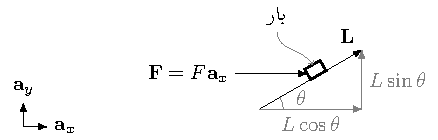
\includegraphics[height=2.5cm]{figBasicFactsWorkAsDotProduct}
\caption{کارتیسی نظام میں کام}
\label{شکل_حقائق_کارتیسی_کام}
\end{figure}
جہاں پچھلی مثال کی مدد سے \عددیء{\ax \cdot \ax=1} اور \عددیء{\ax \cdot \ay=0} لی گئی ہیں۔ یہی جواب ضربِ نقطہ کی تعریف یعنی مساوات سے با آسانی حاصل ہوتا ہے۔
\انتہا{مثال}
%
\حصہ{تفرق  اور جُزوی تفرق}
مساوات میں ایک تفاعل جس میں مقررہ ہے کا تفرق دیا گیا ہے جبکہ مساوات  میں ایک تفاعل کا جُزوی تفرق  دیا گیا ہے۔
\begin{gather}
\begin{aligned}
B (\theta )&=B_0 \cos \theta\\
\frac{\dif B}{\dif \theta}&=-B_0 \sin \theta
\end{aligned}
\end{gather} 
%
\begin{align}
\partial W(x,\lambda)=\frac{\partial W}{\partial x} \dif x+\frac{\partial W}{\partial \lambda} \dif \lambda
\end{align}

\حصہ{خطی تکمل}
مساوات  میں ایک تفاعل \عددیء{B(\theta)} دیا گیا ہے جسے شکل \حوالہ{شکل_حقائق_کوسائن_موج}  میں دکھایا گیا ہے۔ اس کی طولِ موج  \عددیء{2 \pi} ریڈیئن کے برابر ہے۔ ہم \عددیء{-\pi/2<\theta<\pi/2} کے مابین اس کا اوسط معلوم کرتے ہیں۔ یہ تکمل سے یوں ہو گا۔
\begin{align}
B(\theta)=B_0 \cos \theta
\end{align}
%
\begin{align}
B_{\textup{اوسط}}=\frac{B_0}{\pi}\int_{-\frac{\pi}{2}}^{\frac{\pi}{2}} \cos \theta \dif \theta=\frac{2 B_0}{\pi}
\end{align}
اسی طرح اگر اسی خطہ پر تفاعل کے مربع یعنی \عددیء{B^2}  کا اوسط درکار ہو تو ایسا کرنا مساوات میں دکھایا گیا ہے۔
\begin{gather}
\begin{aligned}
B^2_{\textup{اوسط}}&=\frac{B_0^2}{\pi}\int_{-\frac{\pi}{2}}^{\frac{\pi}{2}} \cos^2 \theta \dif \theta\\
&=\frac{B_0^2}{\pi}\int_{-\frac{\pi}{2}}^{\frac{\pi}{2}}\frac{1+\cos 2 \theta}{2} \dif \theta\\
&=\frac{B_0^2}{2}
\end{aligned}
\end{gather}
تفاعل کے مربع کی اوسط کا جزر  بہت اہمیت رکھتا ہے۔لہٰذا اس تفاعل کے مربع کی اوسط کا جزر \عددیء{B_{rms}} مساوات  کی مدد سے یوں حاصل ہوتا ہے۔
\begin{align}
B_{rms}=\sqrt{B^2_{\textup{اوسط}}}=\frac{B_0}{\sqrt{2}}
\end{align}
یہ ایک بہت اہم نتیجہ ہے جو آپ کو زبانی یاد ہونا چاہئے۔ یہ مساوات ہر سائن نما تفاعل کے لئے درست ہے۔کسی بھی متغیرہ کے مربع کی اوسط کا جزر اس متغیرہ کا موثر قیمت کہلاتا ہے۔
%
\begin{figure}
\centering
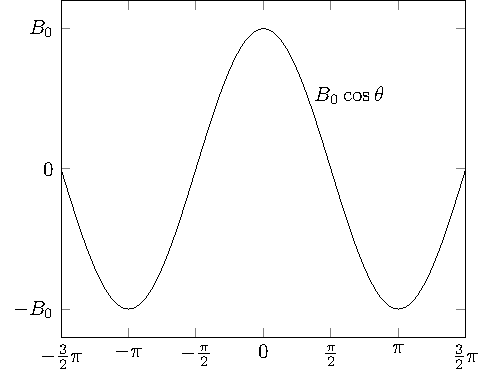
\includegraphics{figBasicFactsCosineWave}
\caption{کوسائن موج}
\label{شکل_حقائق_کوسائن_موج}
\end{figure}
\حصہ{سطحی تکمل}
مثال کے طور پر اگر مساوات  شکل  \حوالہ{شکل_حقائق_نلکی_سطحی_تکمل} میں نلی کے بیرونی سطح پر متغیرہ \عددیء{B} کی مقدار بتلاتی ہے اور یہ متغیرہ سطحی کثافت کو ظاہر کرے  ہم آدھے بیرونی سطح مثلاً زاویہ \عددیء{-\pi/2} اور \عددیء{\pi/2} کے مابین اس کی کُل مقدار \عددیء{\phi} معلوم کرتے ہیں۔اس سطح میں نلی کے دونوں سرے شامل نہیں ہیں۔

	ہم نلی کے بیرونی سطح پر رقبہ  \عددیء{\Delta A} لیتے ہیں جس کی قوسِ صغیرہ \عددیء{\rho \Delta\theta}  اور لمبائی \عددیء{l} ہے۔یہ سطح \عددیء{abcd} ہے۔\عددیء{\Delta \theta} کو نہایت کم کرتے ہوئے سطح کا رقبہ \عددیء{\rho l \dif \theta} لکھا جا سکتا ہے۔چونکہ اس سطح پر \عددیء{B} کی مقدار محوری لمبائی  کی جانب تبدیل نہیں ہو رہی اس لئے سطح \عددیء{\Delta A}  پر \عددیء{\Delta \phi=B \Delta A} ہو گا اور کُل \عددیء{\phi} تکمل کی مدد سے یوں حاصل ہو گا۔
\begin{figure}
\centering
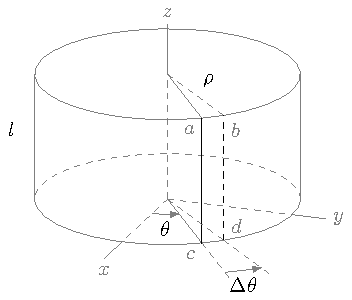
\includegraphics{figBasicFactsCylindricalSurfaceIntegral}
\caption{نلی کی بیرونی سطح پر متغیرہ کا تکمل کُل مقدار دے گی۔}
\label{شکل_حقائق_نلکی_سطحی_تکمل}
\end{figure}
%
\begin{align}
\Delta \phi=B \Delta A=B_0 l \rho \cos \theta \dif \theta
\end{align}
%
\begin{align}
\phi = B_0 l \rho \int_{-\pi/2}^{\pi/2} \cos \theta \dif \theta =2 B_0 l \rho
\end{align}
اب ہم یہی مقدار نلی کے آدھے بیرونی سطح پر کہیں پر بھی حاصل کرنا چاہیں تو ہمیں صرف تکمل کے دو حد تبدیل کرنے ہوں گے۔  اگر ہم مساوات  میں نچلا حد \عددیء{(-\pi/2-\alpha)} اور اُوپر کا حد \عددیء{(\pi/2-\alpha)} لیں تو یہ حاصل ہوگا۔
\begin{align}
\phi (\alpha) = B_0 l \rho \int_{-\frac{\pi}{2}-\alpha}^{\frac{\pi}{2}-\alpha} \cos \theta \dif \theta =2 B_0 l \rho \cos \alpha
\end{align}
یہاں  \عددیء{\phi(\alpha)} اس بات کو واضح کرتا ہے کہ نتیجہ \عددیء{\alpha} پر منحصر ہے۔ یہ ایک بہت اہم مساوات ہے۔ مساوات میں  اگر \عددیء{\alpha=0} ہو تو مساوات   ملتا ہے۔

\حصہ{ دوری سمتیہ}
\begin{figure}
\centering
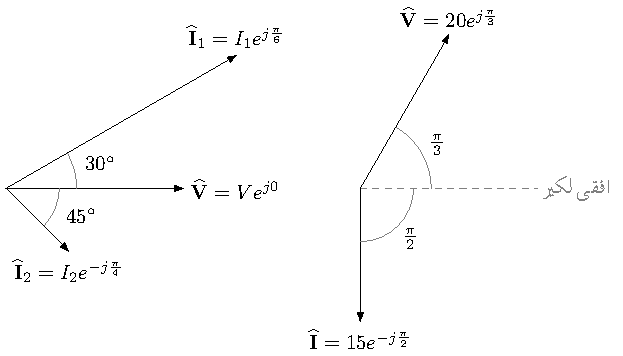
\includegraphics{figBasicFactsPhasors}
\caption{دوری سمتیہ}
\label{شکل_حقائق_دوری_سمتیات}
\end{figure}
سائن نما موج جن کا تعدد معین ہو کو دوری سمتیہ سے ظاہر کرنا نہایت مفید ثابت ہوتا ہے۔ مساواتِ یولر
\begin{align}
A_0 e^{\mp j (\omega t + \phi)}=A_0 \cos (\omega t +\phi) \mp j \sin (\omega t+\phi)
\end{align}
کی مدد سے کو-سائن موج یوں لکھی جا سکتی ہے
\begin{align}
A_0 \cos (\omega t +\phi)=\frac{A_0}{2} \left(e^{j(\omega t +\phi)} -e^{-j(\omega t +\phi)}\right)
\end{align}
اس سے ثابت ہوتا ہے کہ کو-سائن موج دراصل دو مخلوط اعداد کا مجموعہ ہے۔ مساواتِ یولر ایک مخلوط عدد کو ظاہر کرتا ہے جس کے دو جُز ہیں۔ اس کا ایک جُز حقیقی عدد ہے اور اس کا دوسرا جُز فرضی عدد ہے۔اس کا حقیقی جُز کو-سائن موج کو ظاہر کرتا ہے۔ لہٰذا ایک کو-سائن موج  \عددیء{A_0 e^{j(\omega t +\phi)}} یا \عددیء{A_0 e^{-j(\omega t +\phi)}} کا حقیقی جُز ہوتا ہے۔ رسمی طور پر سائن نما موج کو \عددیء{A_0 e^{j(\omega t +\phi)}} سے ظاہر کیا جاتا ہے۔ مزید یہ کہ اس عدد کو چھوٹا کر کے صرف \عددیء{A_0 e^{j\phi}} یا پھر \عددیء{A_0 \phase{\phi}} لکھا جاتا ہے۔کو-سائن موج کے اس طرح ظاہر کرنے کو دوری سمتیہ کہتے ہیں جہاں اس سمتیہ کا طول \عددیء{A_0} اور اُفقی لکیر سے زاویہ \عددیء{\phi} ہے۔

	 دوری سمتیہ استعمال کرتے وقت آپ کو یہ ذہن میں رکھنا ہوتا ہے کہ یہ ایک کو-سائن موج ہے جس کا حیطہ  \عددیء{A_0} ، دوری زاویہ \عددیء{\phi} اور زاویاتی تعدد \عددیء{\omega} ہے۔

اس کتاب میں دوری سمتیہ کو سادہ طرزِ لکھائی میں انگریزی کے بڑے حروف جن پر ٹوپی کا نشان ہو سے ظاہر کیا جائے گا، یعنی \عددیء{\hat{I},\hat{V}}  وغیرہ اور ان کے طول کو بغیر ٹوپی کے نشان کے اسی حرف سے ظاہر کیا جائے گا۔مثلاً برقی دباؤ \عددیء{v= 20 \cos (\omega t +\frac{\pi}{3})} کے لئے یہ سب درست ہیں۔
\begin{gather}
\begin{aligned}
v&=20 \cos (\omega t +\frac{\pi}{3})\\
\hat{V}&=20 e^{j \frac{\pi}{3}}\\
\hat{V}&=20 \phase{\frac{\pi}{3}}\\
V&=20
\end{aligned}
\end{gather}
اس مساوات میں پہلا جُز ایک عام کوسائن موج ہے۔ دوسرا جُز اِسی کو دوری سمتیہ سے ظاہر کر رہا ہے۔ تیسرا اس دوری سمتیہ کا طول اور چوتھا اس کا زاویہ بتلا رہا ہے۔
\begin{figure}
\centering
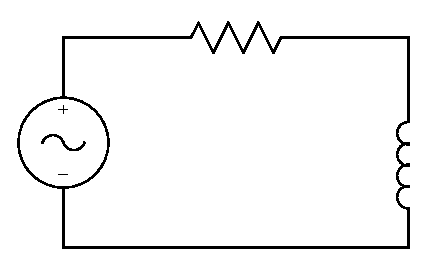
\includegraphics{figBasicFactsRLcircuit}
\caption{دوری سمتیہ کی مدد سے \عددیء{RL} دور کا حل۔}
\label{شکل_حقائق_دوری_سمتیہ_سے_دور_حل}
\end{figure}
	دوری سمتیہ کو عام سمتیوں کی طرح ہی تصور کیا جاتا ہے۔ اس مساوات میں \عددیء{\hat{V}} کا طول \عددیء{20} اور اُفقی لکیر سے زاویہ  \عددیء{\tfrac{\pi}{3}} ریڈیئن ہے۔زاویہ اُفقی لکیر سے گھڑی کی اُلٹی سمت ناپا جاتا ہے۔ اس سمت میں زاویہ مثبت ہے۔ شکل \حوالہ{شکل_حقائق_دوری_سمتیات} میں اسے اور چند اور دوری سمتیہ دکھائے گئے ہیں۔

برقی دور حل کرتے وقت برقی دباؤ \عددیء{\hat{V}} کو اُفقی سمت میں بنا کر برقی رو  \عددیء{\hat{I}} اس کی نسبت سے بنایا جاتا ہے۔شکل \حوالہ{شکل_حقائق_دوری_سمتیات}   میں \عددیء{\hat{I_1}} تیس درجہ زاویہ برقی دباؤ سے آگے  ہے جبکہ  \عددیء{\hat{I_2}}  پینتالیس درجہ زاویہ اس کے پیچھے  ہے۔یہاں یہ دھیان رہے کہ شکل میں  \عددیء{45\degree} مثبت لکھا گیا ہے۔چونکہ یہ اُفقی لکیر سے زاویہ ناپنے کی اُلٹ سمت میں ہے لہٰذا یہ ایک منفی زاویہ ہے۔

یہاں دوری سمتیوں کو استعمال کر کے ایک سادہ برقی دور حل کرتے ہیں۔ یوں ان سے وابستگی پیدا ہو جائے گی اور ان کا استعمال بھی سیکھ لیں گے۔

شکل   ایک سادہ \عددیء{R-L} برقی دور ہے جس پر لاگو برقی دباؤ
\begin{gather}
\begin{aligned}
v(t)&=V_0 \cos (\omega t +\alpha)\\
\hat{V}&=V_0 \phase{\alpha}
\end{aligned}
\end{gather}
ہے۔دوری سمتیہ کے استعمال سے ہم اس میں برقی رو \عددیء{i(t)} معلوم کرنا چاہتے ہیں۔
\begin{gather}
\begin{aligned}
\hat{I}&=\frac{\hat{V}}{R+j X}=\frac{V_0 \phase{\alpha}}{\abs{Z} \phase {\phi_Z}}\\
&=\frac{V_0}{\abs{Z}} \phase{\alpha-\phi_Z}=I_0 \phase{\alpha-\phi_Z}
\end{aligned}
\end{gather}
جہاں \عددیء{\phi_Z} مقاومت کا زاویہ  ہے۔لہٰذا
\begin{align}
i(t)=I_0 \cos (\omega t +\alpha-\phi_Z)
\end{align}


%\باب{مقناطیسی ادوار}
\حصہ{مزاحمت  اور ہچکچاہٹ}
شکل \حوالہ{شکل_مقناطیسی_دور_مزاحمت_ہچکچاہٹ}  میں ایک سلاخ دکھائی گئی ہے۔ اس کی لمبائی کی سمت میں مزاحمت  یہ ہے
\begin{align}
R=\frac{l }{\sigma A}
\end{align}
جہاں  \عددیء{\sigma} موصلیت کو ظاہر کرتی ہے اور \عددیء{A=wh}  ہے۔
\begin{figure}
\centering
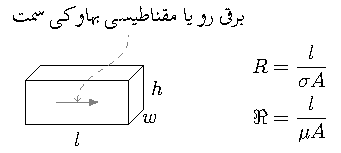
\includegraphics{figMagneticCircuitsResistanceAndReluctance}
\caption{مزاحمت اور ہچکچاہٹ}
\label{شکل_مقناطیسی_دور_مزاحمت_ہچکچاہٹ}
\end{figure}
اگر اس سلاخ کا مقناطیسی مستقل\فرہنگ{مقناطیسی مستقل}\حاشیہب{permeability, magnetic constant}\فرہنگ{permeability}\فرہنگ{magnetic constant}  \عددیء{\mu} ہو تو اس سلاخ کی ہچکچاہٹ\فرہنگ{ہچکچاہٹ}\فرہنگ{reluctance}\حاشیہب{reluctance} \عددیء{\Re}  یوں بیان کی جائے گی۔
\begin{align}
\Re = \frac{l}{\mu A}
\end{align}
مقناطیسی مستقل \عددیء{\mu} کو عموما ً خالی خلاء کی مقناطیسی مستقلکی \عددیء{\mu_0} نسبت سے لکھا جاتا ہے یعنی
\begin{align}
\mu=\mu_r \mu_0
\end{align}
جہاں \عددیء{\mu_r} جزو مقناطیسی مستقل\فرہنگ{مقناطیسی مستقل!جزو}\فرہنگ{relative permeability}\فرہنگ{permeability!relative}  کہلاتی ہے۔ہچکچاہٹ کی اکائی ایمپیئر-چکر فی ویبر  ہے جس کی وضاحت آپ کو جلد ہو جائے گی۔
%
\ابتدا{مثال}
شکل  میں دی گئی سلاخ کی ہچکچاہٹ معلوم کریں
\عددیء{\mu_r=2000 }، \عددیء{l=\SI{10}{\centi \meter}}، \عددیء{h=\SI{3}{\centi \meter}} اور \عددیء{w=\SI{2.5}{\centi \meter}} ہیں۔

حل:
\begin{align*}
\Re& = \frac{l}{\mu_r \mu_0 A}\\
&=\frac{10\times 10^{-2}}{2000 \times 4 \pi \times 10^{-7} \times 2.5 \times 10^{-2} \times 3 \times 10^{-2}}\\
&=\SI{53044}{\ampere \cdot turns \per \weber}
\end{align*}
\انتہا{مثال}

\حصہ{کثافتِ برقی رو  اور برقی میدان کی شدت}
اگر اس سلاخ کے سروں پر برقی دباؤ \عددیء{v} لاگو کی جائے جیسا کہ شکل  \حوالہ{شکل_مقناطیسی_دور_کثافت_رو_اور_برقی_شدت} میں دکھایا گیا ہے تو اس میں برقی رو \عددیء{i} گزرے گا جس کی مقدار اوہم کے قانون  سے یوں حاصل ہوتی ہے
\begin{align}
i=\frac{v}{R}
\end{align}
اس مساوات کو مساوات  کی مدد سے یوں لکھ سکتے ہیں
\begin{align}
i=v \left(\frac{\sigma A}{l}\right)
\end{align}
یا
\begin{align}
\frac{i}{A}=\sigma \left(\frac{v}{l} \right)
\end{align}
اسے مزید یوں لکھ سکتے ہیں
\begin{align}
J =\sigma E
\end{align}
اگر شکل میں سمتیہ \سمتیہ{J} کا طول \عددیء{J} ہو اور سمتیہ \سمتیہ{E} کا طول \عددی{E} ہو جہاں ان دونوں سمتیہ کی سمت  \عددیء{\ay} ہے تب  اس مساوات کو یوں لکھا جا سکتا ہے۔
\begin{align}
\kvec{J}=\sigma \kvec{E}
\end{align}
یہ دونوں مساوات اوہم کے قانون کی ایک اور شکل ہیں۔ مساوات  میں 
\begin{align}
J&=\frac{i}{A}\\
E&=\frac{v}{l}
\end{align}
%
\begin{figure}
\centering
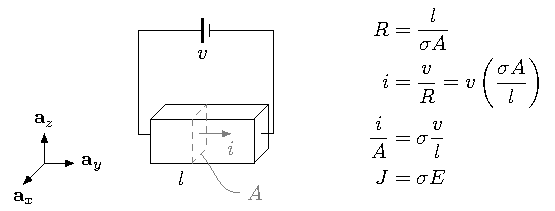
\includegraphics{figMagneticCircuitsCurrentDensityAndElectricFieldIntensity}
\caption{کثافتِ برقی رو اور برقی دباؤ کی شدت}
\label{شکل_مقناطیسی_دور_کثافت_رو_اور_برقی_شدت}
\end{figure}
ہیں۔ شکل سے واضح ہے کہ برقی رو \عددیء{i} سلاخ کی رقبہ عمودی تراش \عددیء{A} سے گزرتی ہے لہٰذا مساوات کے تحتب \عددیء{J} رقی رو کی کثافت کو ظاہر کرتی ہے۔ اسی وجہ سے \عددیء{J} کو کثافتِ برقی رو \فرہنگ{کثافت!برقی رو}\حاشیہب{current density} ہی کہتے ہیں۔ اسی طرح مساوات   سے یہ واضح ہے کہ \عددیء{E} برقی دباؤ فی اکائی لمبائی کو ظاہر کرتی ہے۔  یوں  \عددیء{E} کو برقی میدان کی شدت\فرہنگ{برقی میدان!شدت}\حاشیہب{electric field intensity} کہتے ہیں۔جہاں متن سے واضح ہو کہ برقی میدان کی بات ہو رہی ہے وہاں اس نام کو چھوٹا کر کے \عددیء{E} کو میدانی شدت  سے پکارا جاتا ہے۔برقی میدان\فرہنگ{برقی میدان}\حاشیہب{electric field}\فرہنگ{electric field} سے مُراد کسی چارج کے اِردگرد وہ جگہ ہے جس میں اس چارج کا اثر محسوس کیا جاتا ہے۔

	ہم بالکل اسی طرح مقناطیسی متغیرہ کے لئے بھی اس طرح کے مساوات لکھ سکتے ہیں۔ حصہ  میں بھی یہی کریں گے۔

\حصہ{برقی ادوار}
	برقی دور میں برقی دباؤ\فرہنگ{برقی دباو}\حاشیہب{electric voltage}  \عددیء{V}  کی وجہ سے برقی رو\فرہنگ{برقی رو}\حاشیہب{electric current} \عددیء{i} پیدا ہوتی ہے۔ تانبہ\فرہنگ{تانبہ}\حاشیہب{copper}   کی موصلیت \عددیء{\sigma=\SI{5.9e7}{\siemens \per \meter}} ہے جہاں \عددیء{\si{\siemens \per \meter}} موصلیت کی اکائی ہے۔لہٰذا تانبہ کی بنی تار کی مزاحمت  \عددیء{R_{\textup{تار}}}  قابلِ نظرانداز ہوتی ہے۔اگر ایسی تار میں برقی رو \عددیء{i} کا گزر ہو  تو اس تار کی مزاحمت میں اوہم کے قانون کے تحت  برقی دباؤ  \عددیء{\Delta v=i R_{\textup{تار}}} گھٹے  گی۔\عددیء{R_{\textup{تار}}} کی قابلِ نظر انداز ہونے کی وجہ سے یہ مقدار بھی قابلِ نظر انداز ہی ہو گی۔ اس کا مطلب ہے کہ برقی تار کی مدد سے برقی دباؤ کی ایک جگہ سے دوسری جگہ رسائی بغیر کم ہوئے ممکن ہے۔اسی لئے تانبہ کی تار کو عموما ً برقی دباؤ کی ایک جگہ سے دوسری جگہ رسائی کے لئے استعمال کیا جاتا ہے اور اس کی مزاحمت کو صفر ہی سمجھا جاتا ہے۔ شکل الف میں ایک ایسا ہی برقی دور دکھایا گیا ہے۔اس برقی دور میں کُل تار کی مزاحمت \عددیء{R_{\textup{تار}}} ہے۔ اگر تار کی مزاحمت کو نظرانداز کیا جا سکے تو ہمیں برقی دور حصہ ب ملتا ہے۔اس برقی دور میں برقی دباؤ \عددیء{v} کو مزاحمت \عددیء{R} تک بغیر کم کئے پہنچایا گیا ہے۔
\begin{figure}
\centering
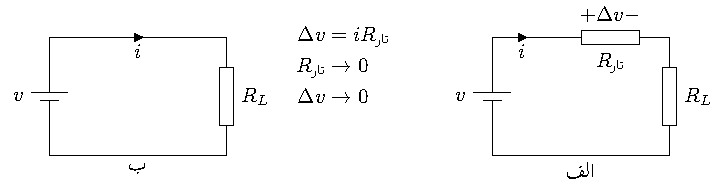
\includegraphics{figMagneticCircuitsResistiveSeriesCircuit}
\caption{برقی دور میں تار کی مزاحمت کو نظر انداز کیا جاتا ہے۔}
\label{شکل_مقناطیسی_دور_سلسہ_وار_مزاحمتی_ادوار}
\end{figure}
%---------------------
\begin{figure}
\centering
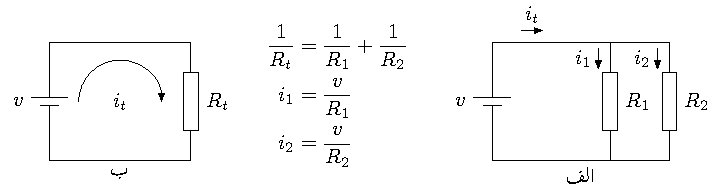
\includegraphics{figMagneticCircuitsResistiveParallelCircuit}
\caption{برقی رو کم مزاحمت کے راستے  زیادہ ہوتی ہے}
\label{شکل_مقناطیسی_دور_متوازی_مزاحمتی_دور}
\end{figure}
%

شکل \حوالہ{شکل_مقناطیسی_دور_متوازی_مزاحمتی_دور}  میں ایک اور مثال دی گئی ہے۔ یہاں ہم دیکھتے ہیں کہ برقی رو اس راستے زیادہ ہوتی ہے جس کی مزاحمت کم ہو۔ لہٰذا اگر \عددیء{R_1 < R_2}ہو تو \عددیء{i_1>i_2} ہو گی۔

\حصہ{مقناطیسی دور حصہ اول}
مقناطیسی دور بالکل برقی دور کی طرح ہوتے ہیں۔ بس ان میں برقی دباؤ \عددیء{v} کی جگہ مقناطیسی دباؤ \عددیء{\tau} ، برقی رو \عددیء{i}  کی جگہ مقناطیسی بہاؤ \عددیء{\phi}  اور مزاحمت \عددیء{R} کی جگہ  ہچکچاہٹ  \عددیء{\Re} ہوتی ہے۔ لہٰذا ہم بالکل ایک برقی دور کی طرح ایک مقناطیسی دور بنا سکتے ہیں۔ ایسا ہی ایک دور شکل \حوالہ{شکل_مقناطیسی__مقناطیسی_سلسلہ_وار_دور}-الف میں دکھایا گیا ہے۔
\begin{figure}
\centering
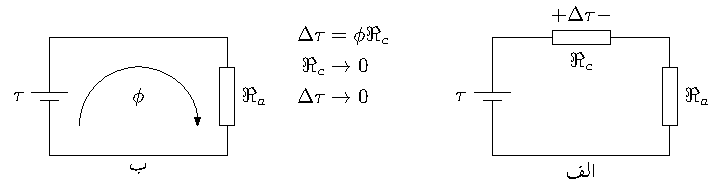
\includegraphics{figMagneticCircuitsReluctanceSeriesCircuit}
\caption{مقناطیسی دور}
\label{شکل_مقناطیسی__مقناطیسی_سلسلہ_وار_دور}
\end{figure}
%
یہاں بھی کوشش یہی ہے کہ کسی طرح مقناطیسی دباؤ \عددیء{\tau} کو بغیر کم کئے ہچکچاہٹ \عددیء{\Re_a} تک پہنچایا جائے۔ عموما ً \عددیء{\Re_a} خلائی درز کی ہچکچاہٹ ہوتی ہے اور \عددیء{\Re_c} مقناطیسی مرکز کی۔ یہاں بھی اگر \عددیء{\Re_c} کو نظرانداز کرنا ممکن ہو تو ہمیں شکل \حوالہ{شکل_مقناطیسی__مقناطیسی_سلسلہ_وار_دور}-ب ملتا ہے جس میں مقناطیسی بہاؤ \عددیء{\phi} کو، بالکل اوہم کے قانون کی طرح، مساوات سے حل کیا جا سکتا ہے۔ یعنی
\begin{align}
\tau=\phi \Re_a
\end{align}
 اگر \عددیء{\Re_c} کو نظرانداز کرنا ممکن نہ ہو تب بالکل سلسلہ وار مزاحمتوں کی طرح ہم اس شکل میں دیئے گئے دو سلسلہ وار ہچکچاہٹوں کا مجموعہ ہچکچاہٹ  \عددیء{\Re_s} کو استعمال کر کے برقی رو کا حساب لگائیں گے، یعنی
\begin{align}
\Re_s&=\Re_a+\Re_c\\
\tau&=\phi \Re_s
\end{align}
	بالکل برقی مثال کی طرح، مقناطیسی دباؤ کو کم ہچکچاہٹ والے راستے سے اس جگہ پہنچایا جاتا ہے جہاں اس کی ضرورت ہو۔ مساوات سے ہم دیکھتے ہیں کہ ہچکچاہٹ،  مقناطیسی مستقل \عددیء{\mu} سے منسلک ہے ۔\عددیء{\mu} کو عموما ً \عددیء{\mu=\mu_r \mu_0} لکھا جاتا ہے جہاں  \عددیء{\mu_0=4 \pi \times 10^{-7}} ہینری فی میٹر\حاشیہب{Henry per meter}  کے برابر ہے۔ لوہا،  کچھ دھاتیں اور چند جدید مصنوعی اشیاء  ایسی ہیں جن کی \عددیء{2000 < \mu_r < 80000} ہے۔ لہٰذا انہیں کو مقناطیسی دباؤ  ایک جگہ سے دوسری جگہ منتقلی کے لئے استعمال کیا جاتا ہے۔ البتہ \عددیء{\mu} کی مقدار اتنی نہیں ہے کہ اس سے بنی سلاخ کی ہچکچاہٹ ہر جگہ نظرانداز کی جا سکے۔ مساوات  سے ہم دیکھتے ہیں کہ ہچکچاہٹ کم سے کم کرنے کی خاطر رقبہ عمودی تراش زیادہ سے زیادہ رکھنی پڑتی ہے۔ لہٰذا عموما ً مقناطیسی دباؤ منتقل کرنے کے لئے ایک تار نہیں بلکہ خاصی زیادہ سطح عمودی تراش رکھنے والا راستہ  درکار ہوتا ہے جسے مقناطیسی مرکز\فرہنگ{مقناطیسی مرکز}\حاشیہب{magnetic core}\فرہنگ{magnetic core} کہتے ہیں۔برقی آلوں میں استعمال  مقناطیسی مرکز لوہے کی باریک چادر یا پتری\فرہنگ{پتری}\حاشیہب{laminations}\فرہنگ{laminations}  تہہ  در تہہ رکھ کر بنائی جاتی ہے۔ مقناطیسی مرکز کے بارے میں ہم حصہ  میں مزید معلومات حاصل کریں گے۔

\حصہ{کثافتِ مقناطیسی بہاؤ  اور مقناطیسی میدان کی شدت}
حصہ  میں ہم نے برقی مثال دی۔ یہاں ہم مقناطیسی مثال پیش  کرتے ہیں۔ شکل \حوالہ{شکل_مقناطیسی__کثافت_مقناطیسی_بہاو_اور_شدت} میں ایک مقناطیسی مثال دکھائی گئی ہے۔یہاں مقناطیسی مرکز کی \عددیء{\mu_r = \infty} تصور کی گئی ہے لہٰذا اس مرکز کی ہچکچاہٹ \عددیء{\Re_c} صفر ہو گی۔ لہٰذا جیسے حصہ  میں تانبہ کی تار استعمال کی گئی تھی یہاں اسی طرح مقناطیسی مرکز کو مقناطیسی دباؤ \عددیء{\tau} ایک جگہ سے دوسری جگہ منتقل کرنے کے لئے استعمال کیا گیا ہے۔ اس شکل میں مقناطیسی دباؤ کو خلائی درز کی ہچکچاہٹ \عددیء{\Re_a} تک پہنچایا گیا ہے۔
\begin{figure}
\centering
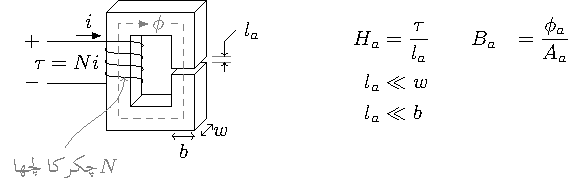
\includegraphics{figMagneticCircuitsMagneticFluxDensityAndIntensity}
\caption{کثافتِ مقناطیسی بہاؤ اور مقناطیسی میدان کی شدت}
\label{شکل_مقناطیسی__کثافت_مقناطیسی_بہاو_اور_شدت}
\end{figure}

لہٰذا یہاں کُل ہچکچاہٹ صرف خلائی درز کی ہچکچاہٹ ہی ہے یعنی
\begin{align}
\Re_a=\frac{l_a}{\mu_0 A_z}
\end{align}
خلائی درز کے رقبہ عمودی تراش \عددیء{A_a} کو مرکز کے رقبہ عمودی تراش \عددیء{\Re_c} کے برابر لیا گیا ہے۔ یعنی 
\begin{align}
A_a=A_c=w b
\end{align}
اگر خلائی درز کی لمبائی \عددیء{l_a} مرکز کے رقبہ کے اطراف \عددیء{b} اور \عددیء{w} سے نہایت کم ہو یعنی \عددیء{l_a \ll b} اور \عددیء{l_a \ll w} تب ایسا کرنا ممکن ہوتا ہے۔ اس کتاب میں یہی تصور کیا جائے گا۔

مقناطیسی دباؤ کو یوں بیان کیا جاتا ہے
\begin{align}
\tau=N i
\end{align}
یعنی برقی تار کے چکر ضربِ ان میں برقی رو۔ لہٰذا مقناطیسی دباؤ کی اکائی ایمپیئر-چکر\فرہنگ{ایمپیئر-چکر}\حاشیہب{ampere-turn}\فرہنگ{ampere-turn}  ہے۔ بالکل حصہ  کی طرح ہم مساوات کو یوں لکھ سکتے ہیں۔
\begin{align}
\phi_a=\frac{\tau}{\Re_a}
\end{align}
مقناطیسی بہاؤ کی اکائی ویبر\فرہنگ{ویبر}\حاشیہب{Weber}\فرہنگ{Weber}\حاشیہد{یہ اکائی جرمنی کے ولیم اڈورڈ ویبر کے نام ہے جن کا برقی و مقناطیسی میدان میں اہم کردار رہا ہے}  ہے اور ہچکچاہٹ کی اکائی ایمپیئر-چکر فی ویبر\حاشیہب{ampere-turn per weber} ہے۔  خلائی درز میں مقناطیسی بہاؤ \عددیء{\phi_a} اور مرکز میں مقناطیسی بہاؤ \عددیء{\phi_c} برابر ہیں۔ اس مساوات کو مساوات   کی مدد سے یوں لکھ سکتے ہیں۔
\begin{align}
\phi_a &=\tau \left(\frac{\mu_0 A_a}{l_a} \right)\\
\frac{\phi_a}{A_a}&=\mu_0 \left( \frac{\tau}{l_a} \right)
\end{align}
	اس مساوات میں بائیں جانب مقناطیسی بہاؤ فی اکائی رقبہ کو کثافتِ مقناطیسی بہاؤ\فرہنگ{مقناطیسی بہاو!کثافت}\حاشیہب{magnetic flux density}\فرہنگ{magnetic flux!density} \عددیء{B_a} اور دائیں جانب برقی دباؤ فی اکائی لمبائی کو مقناطیسی میدان کی شدت\فرہنگ{مقناطیسی میدان!شدت}\حاشیہب{magnetic field intensity}\فرہنگ{magnetic field!intensity}  \عددیء{H_a} لکھا جا سکتا ہے۔یعنی
\begin{align}
B_a&=\frac{\phi_a}{A_a}\\
H_a&=\frac{\tau}{l_a}
\end{align}
کثافتِ مقناطیسی بہاؤ کی اکائی ویبر فی مربہ میٹر ہے جس کو ٹیسلہ\فرہنگ{ٹیسلہ}{Tesla}\فرہنگ{Tesla}\حاشیہد{Tesla:  یہ اکائی سربیا کے نِکولا ٹیسلہ کے نام ہے جنہوں نے بدلتی رو برقی طاقت عام کرنے میں اہم کردار ادا کیا}  کا نام دیا گیا ہے۔مقناطیسی میدان کی شدت کی اکائی ایمپیئر فی میٹر\حاشیہب{ampere per meter}  ہے۔ لہٰذا مساوات کو ہم یوں لکھ سکتے ہیں۔
\begin{align}
B_a=\mu_0 H_a
\end{align}
جہاں متن سے واضح ہو کہ مقناطیسی میدان کی بات ہو رہی ہے وہاں مقناطیسی میدان کی شدت کو میدانی شدت\حاشیہب{field intensity} کہا جاتا ہے۔  شکل میں ہم دیکھتے ہیں کہ خلائی درز میں مقناطیسی بہاؤ کی سمت،  اکائی سمتیہ \عددیء{\az} کی الٹ سمت میں ہے لہٰذا ہم کثافتِ مقناطیسی بہاؤ کو \عددیء{\kvec{B_a}=-B_a \az} لکھ سکتے ہیں۔ اسی طرح خلائی درز میں مقناطیسی دباؤ  اکائی سمتیہ \عددیء{\az} کی الٹ سمت میں دباؤ ڈال رہی ہے لہٰذا ہم مقناطیسی دباؤ کی شدت کو \عددیء{\kvec{H_a}=-H_a \az} لکھ سکتے ہیں۔ لہٰذا اس مساوات کو یوں لکھا جا سکتا ہے۔
\begin{align}
\kvec{B_a}=\mu_0 \kvec{H_a}
\end{align}
اگر خلاء کی جگہ کوئی ایسے مادہ ہو جس کی ہو، تب ہم اس مساوات کو یوں لکھتے
\begin{align}
\kvec{B}=\mu \kvec{H}
\end{align}
%
\ابتدا{مثال}
شکل میں خلائی درز میں کثافتِ مقناطیسی بہاؤ \عددیء{0.1} ٹیسلہ درکار ہے۔مرکز کی \عددیء{\mu_r=\infty}  ہے اور خلائی درز کی لمبائی \عددیء{1} ملی میٹر ہے۔اگر  مرکز کے گرد برقی تار کے \عددیء{100} چکر ہوں تو ان میں درکار برقی رو معلوم کریں۔

حل:
\begin{align*}
\tau&=\phi \Re\\
N i & \phi \left(\frac{l}{\mu_0 A} \right)\\
\frac{\phi}{A}&=\frac{ N i \mu_0}{l}
\end{align*}
لہٰذا
\begin{align*}
0.1&=\frac{100 \times i \times 4 \pi  10^{-7}}{0.001}\\
i&=\frac{0.1 \times 0.001}{100 \times 4 \pi  10^{-7}}=\SI{0.79567}{\ampere}
\end{align*}
یعنی \عددیء{0.79567} ایمپیئر برقی رو سے خلائی درز میں \عددیء{0.1} ٹیسلہ کثافتِ مقناطیسی بہاؤ حاصل ہو جائے گی۔
\انتہا{مثال}
%
\حصہ{مقناطیسی دور حصہ دوم}
شکل \حوالہ{شکل_مقناطیسی__سادہ_مقناطیسی_دور_بغیر_درز} میں ایک سادہ مقناطیسی نظام دکھایا گیا ہے جس میں مرکز کی مقناطیسی مستقل کو محدود تصور کیا گیا ہے۔شکل میں مقناطیسی دباؤ  \عددیء{\tau=N i} مقناطیسی مرکز میں مقناطیسی بہاؤ \عددیء{\phi_c} کو جنم دیتی ہے۔ یہاں مرکز کا رقبہ عمودی تراش \عددیء{A_c}  ہر جگہ یکساں ہے اور مرکز میں  نقطہ دار لکیر کی لمبائی \عددیء{l_c} ہے۔ مرکز میں مقناطیسی بہاؤ  کی سمت فلیمنگ\حاشیہب{Fleming's right hand rule} کے دائیں ہاتھ کے قانون  سے معلوم کی جا سکتی ہے۔  اس قانون کو دو طریقوں سے بیان کیا جا سکتا ہے۔
\begin{itemize}
\item
اگر ایک لچھے کو دائیں ہاتھ سے یوں پکڑا  جائے کہ ہاتھ کی چار انگلیاں لچھے میں برقی رو کی سمت میں لپٹی  ہوں تو انگوٹھا اُس مقناطیسی بہاؤ کی سمت میں ہوگا جو اس برقی رو کی وجہ سے وجود میں آئیگا۔
\item
اگر ایک تار جس میں برقی رو کا گزر ہو، کو دائیں ہاتھ سے یوں پکڑا جائے کہ انگوٹھا  برقی رو  کی سمت میں ہو تو باقی چار انگلیاں اُس مقناطیسی  رو ، جو اس برقی رو کی وجہ سے وجود میں آئے،  کی سمت میں لپٹی ہوں گی۔
\end{itemize}

ان دو بیانات میں پہلا بیان،  لچھے میں مقناطیسی بہاؤ کی سمت معلوم کرنے کے لئے زیادہ آسان ثابت ہوتا ہے جبکہ کسی ایک سیدھی تار کے گرد مقناطیسی بہاؤ کی سمت دوسرے بیان سے زیادہ آسانی سے معلوم کی جا سکتی ہے۔
\begin{figure}
\centering
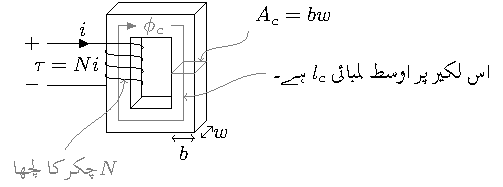
\includegraphics{figMagneticCircuitsSimpleMagneticCircuitNoGap}
\caption{سادہ مقناطیسی دور}
\label{شکل_مقناطیسی__سادہ_مقناطیسی_دور_بغیر_درز}
\end{figure}
لہٰذا مرکز میں مقناطیسی بہاؤ  گھڑی کے سمت میں ہے۔ یہ شکل میں نقطہ دار لکیر پر تیر کے نشان سے ظاہر کیا گیا ہے۔ یہاں مرکز کی ہچکچاہٹ 
\begin{align}
\Re_c&=\frac{l_c}{\mu_c A_c}\\
\phi_c&=\frac{\tau}{\Re_c}=N i \left(\frac{\mu_c A_c}{l_c} \right)
\end{align}
اس طرح ہم سب متغیرات حاصل کر سکتے ہیں۔
%
\ابتدا{مثال}
شکل \حوالہ{شکل_مقناطیسی__درز_اور_ہچکچاہٹ}  میں ایک مقناطیسی مرکز دکھایا گیا ہے جہاں
\begin{align}
\text{کور}= \left\{ 
  \begin{array}{l l}
  h=\SI{20}{\centi\meter} & m=\SI{10}{\centi \meter}\\
 n=\SI{8}{\centi\meter} & w=\SI{2}{\centi \meter}\\
 l_a=\SI{1}{\milli\meter} & \mu_r =40000 \\
 \end{array} \right.
\end{align}
ہیں۔مرکز اور خلائی درز کی ہچکچاہٹیں حاصل کریں۔
\begin{figure}
\centering
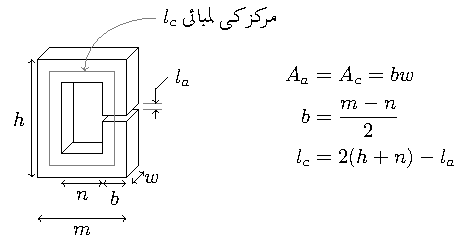
\includegraphics{figMagneticCircuitsCoreWithGapAndReluctance}
\caption{خلائی درز اور مرکز کے ہچکچاہٹ}
\label{شکل_مقناطیسی__درز_اور_ہچکچاہٹ}
\end{figure}
حل:
\begin{align*}
b&=\frac{m-n}{2}=\frac{0.1-0.08}{2}=\SI{0.01}{\meter}\\
A_a&=A_c=bw=0.01 \times 0.02=\SI{0.0002}{\square \meter}\\
l_c&=2(h+n)-l_a=2(0.2+0.08)-0.001=\SI{0.559}{\meter}
\end{align*}
%
\begin{align*}
\Re_c&=\frac{l_c}{\mu_r \mu_0 A_c}=\frac{0.559}{40000 \times 4 \pi 10^{-7} \times 0.0002}=\SI{55598}{\ampere \cdot t \per \weber}\\
\Re_a&=\frac{l_a}{\mu_0 A_a}=\frac{0.001}{4 \pi 10^{-7} \times 0.0002}=\SI{3978358}{\ampere \cdot t \per \weber}
\end{align*}
ہم دیکھتے ہیں اگرچہ مرکز کی لمبائی خلائی درز کی لمبائی سے \عددیء{559} گنا زیادہ ہے تب بھی خلائی درز کی ہچکچاہٹ \عددیء{71} گنا زیادہ ہے یعنی \عددیء{\Re_a  \gg \Re_c} 
\انتہا{مثال}
%
\ابتدا{مثال}
شکل  \حوالہ{شکل_مقناطیسی_دور_سادہ_گھومتا_مشین} سے رجوع کریں۔اگر ایک خلائی درز \عددیء{5} ملی میٹر لمبا ہو اور گھومتے حصہ پر \عددیء{1000} چکر ہوں تو خلائی درز میں \عددیء{0.95} ٹیسلہ کثافتِ برقی بہاؤ حاصل کرنے کی خاطر درکار برقی رو معلوم کریں۔
\begin{figure}
\centering
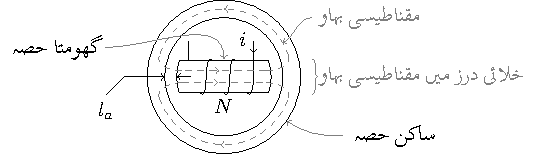
\includegraphics{figMagneticCircuitsSimpleRotatingMachineOutline}
\caption{سادہ گھومنے والا مشین}
\label{شکل_مقناطیسی_دور_سادہ_گھومتا_مشین}
\end{figure}
حل:
	 اس شکل میں ایک گھومتے مشین، مثلاً موٹر، کی ایک سادہ شکل دکھائی گئی ہے۔ ایسے آلوں میں باہر کا حصہ ساکن رہتا ہے جس کو مشین کا ساکن حصہ کہتے ہیں اور اس ساکن حصہ کے اندر اس کا ایک حصہ گھومتا ہے جسے گھومتا حصہ کہتے ہیں۔ اس مثال میں ان دونوں حصوں کا  \عددیء{\mu_r=\infty}  ہے لہٰذا ان کی ہچکچاہٹ صفر ہے۔ مقناطیسی بہاؤ نقطہ دار لکیر سے ظاہر کی گئی ہے۔ یہ خلائی درز میں سے، ایک مکمل چکر کے دوران، دو مرتبہ گزرتی ہے۔ یہ دو خلائی درز ہر لحاظ سے ایک جیسے ہیں لہٰذا ان دونوں خلائی درز کی ہچکچاہٹ بھی برابر ہوں گی۔مزید یہ کہ ان خلائی درز کی ہچکچاہٹ سلسلہ وار ہیں۔شکل میں مقناطیسی بہاؤ کو گھومتے حصہ سے ساکن حصہ کی طرف، خلائی درز سے گزرتے دکھایا گیا ہے۔خلائی درز کی لمبائی \عددیء{l_a} بہت کم ہے لہٰذا خلائی درز کا عمودی رقبہ تراش \عددیء{A_a} وہی ہو گا جو گھومتے حصہ کا ہے یعنی \عددیء{A_c} 

  ایک خلائی درز کی ہچکچاہٹ
\begin{align*}
\Re_a=\frac{l_a}{\mu_0 A_a}=\frac{l_a}{\mu_0 \A_c}
\end{align*}
ہے۔لہٰذا کُل ہچکچاہٹ ہو گی
\begin{align*}
\Re_s=\Re_a=\Re_a=\frac{2 l_a}{\mu_0 A_c}
\end{align*}
یوں خلائی درز میں مقناطیسی بہاؤ \عددیء{\phi_a} اور کثافتِ مقناطیسی بہاؤ \عددیء{B_a} یہ ہوں گے۔
\begin{align*}
\phi_a&=\frac{\tau}{\Re_s}=\left(N i \right) \left (\frac{\mu_0 A_c}{2 l_a} \right)\\
B_a&=\frac{\phi_a}{A_a}=\frac{\mu_0 N i}{2 l_a}
\end{align*}
اس مساوات میں اعداد استعمال کرتے ہیں
\begin{align*}
0.95&=\frac{4 \pi 10^{-7} \times 1000 \times i}{2 \times 0.005}\\
i&=\frac{0.95 \times 2 \times 0.005}{ 4 \pi 10^{-7} \times 1000}=\SI{7.56}{\ampere}
\end{align*}
موٹر اور جنریٹروں کی خلاء میں تقریباً ایک ٹیسلہ کثافتِ برقی بہاؤ ہوتی ہے۔
\انتہا{مثال}

\حصہ{خود امالہ  ، مشترکہ امالہ  اور توانائی}
مقناطیسی بہاؤ کی، وقت کے ساتھ تبدیلی، برقی دباؤ  کو جنم دیتی ہے۔ لہٰذا  اگر شکل  کے مرکز میں مقناطیسی بہاؤ تبدیل ہو رہی ہو تو اس کی وجہ سے اس کے لچھے میں برقی دباؤ پیدا ہوگی جوکہ اس لچھے کے سروں پر نمودار ہوگی۔ اِس طرح پیدا ہونے والی برقی دباؤ کو امالی برقی دباؤ\فرہنگ{امالی برقی دباو}\حاشیہب{induced voltage}\فرہنگ{induced voltage}  کہتے ہیں۔ قانونِ فیراڈے\فرہنگ{فیراڈے!قانون}\حاشیہب{Faraday's law}\فرہنگ{Faraday's law}  کے تحت\حاشیہد{مائکل فیراڈے انکلستانی سائنسدان تھے جنہوں نے محرک برقی دباؤ دریافت کی}
\begin{align}
e=N \frac{\partial \phi}{\partial t} =\frac{\partial \lambda}{\partial t}
\end{align}
اس مساوات میں ہم لچھے میں، وقت کے ساتھ تبدیل ہونے والی، مقناطیسی بہاؤ کو \عددیء{\phi} سے ظاہر کر رہے ہیں۔\عددیء{N \phi} کو لچھے کی اِرتَباطِ بہاؤ\فرہنگ{ارتباط بہاو}\حاشیہب{flux linkage} \عددیء{\lambda}  کہتے ہیں جس کی اکائی ویبر-چکر\فرہنگ{ویبر-چکر}\حاشیہب{weber-turn}  ہے۔ اس امالی برقی دباؤ  کی سمت کا تعین یوں کیا جاتا ہے کہ اگر دیئے گئے لچھے کی سروں کو کسرِ دور\فرہنگ{کسر دور}\حاشیہب{short circuit}   کیا جائے تو اِس میں برقی رو اُس سمت میں ہو گی جس میں مقناطیسی بہاؤ کی تبدیلی کو روکا جا سکے۔ 

جن مقناطیسی دوروں میں مقناطیسی مستقل \عددیء{\mu}  کو اٹل مقدار تصور کیا جا سکے یا جن میں خلائی درز کی ہچکچاہٹ مرکز کی ہچکچاہٹ سے بہت زیادہ ہو یعنی \عددیء{\Re_a \gg \Re_c} ، ان حالات میں ہم لچھے کی  امالہ\فرہنگ{امالہ}\حاشیہب{inductance}\فرہنگ{inductance} \عددیء{L}  کو یوں بیان کرتے ہیں۔
\begin{align}
L=\frac{\lambda}{i}
\end{align}

امالہ کی اکائی ویبر-چکر فی ایمپیئر ہے جس کو ہینری\فرہنگ{Henry}\حاشیہب{Henry}\فرہنگ{Henry} \عددیء{H} کا نام\حاشیہد{امریکی سائنسدان جوزف ہینری جنہوں نے مائکل فیراڈے سے علیحدہ  طور پر محرک برقی دباؤ دریافت کی} دیا گیا ہے۔ لہٰذا
\begin{align}
L=\frac{N \phi}{i}=\frac{N B_c A_c}{i}=\frac{N^2 \mu_0 A_a}{l_a}
\end{align}
%
\ابتدا{مثال}
شکل میں اگر \عددیء{b=\SI{5}{\centi \meter},w=\SI{4}{\centi\meter},l_a=\SI{3}{\milli \meter}} جبکہ لچھے کے \عددیء{1000} چکر اور مرکز کے گرد اوسط لمبائی \عددیء{l_c=\SI{30}{\centi\meter}} ہو تب ان دو صورتوں میں لچھے کی امالہ معلوم کریں۔
\begin{itemize}
\item
مرکز کی \عددیء{\mu_r = \infty} ہے۔
\item
مرکز کی \عددیء{\mu_r = 500} ہے۔
\end{itemize}

حل:
	پہلی صورت میں مرکز کی \عددیء{\mu_r=\infty} ہونے کی وجہ سے مرکز کی ہچکچاہٹ نظرانداز کی جا سکتی ہے۔یوں
\begin{align*}
L&=\frac{N^2 \mu_0 w b}{l_a}\\
&=\frac{1000^2 \times 4 \pi 10^{-7} \times 0.04 \times 0.05}{0.003}\\
&=\SI{0.838}{\henry}
\end{align*}
	دوسری صورت میں \عددیء{\mu_r=500} ہے۔یوں مرکز کی ہچکچاہٹ صفر نہیں۔خلاء اور مرکز کی ہچکچاہٹ پہلے دریافت کرتے ہیں
\begin{align*}
\Re_a&=\frac{l_a}{\mu_0 w b}=\frac{0.003}{4\pi 10^{-7} \times 0.04 \times 0.05}=\SI{1193507}{\ampere \cdot t \per \weber}\\
\Re_c&=\frac{l_c}{\mu_r \mu_0 w b}=\frac{0.3}{500 \times 4\pi 10^{-7} \times 0.04 \times 0.05}=\SI{238701}{\ampere \cdot t \per \weber}
\end{align*}
لہٰذا
\begin{align*}
\phi&=\frac{N i}{\Re_a+\Re_c}\\
\lambda &= N \phi = \frac{N^2 i}{\Re_a+\Re_c}\\
L&=\frac{\lambda}{i}=\frac{N^2}{\Re_a+\Re_c}=\frac{1000^2}{1193507+238701}=\SI{0.698}{\henry}
\end{align*}
\انتہا{مثال}
%
\ابتدا{مثال}
شکل \حوالہ{شکل_مقناطیسی_ادوار_پیچدار_لچھا} میں ایک پیچدار لچھا\فرہنگ{لچھا!پیچدار}\حاشیہب{spiral coil} دکھایا گیا ہے جس کی تفصیل یوں ہے

\عددیء{N=11, r=\SI{0.49}{\meter},l=\SI{0.94}{\meter}}

ایسے پیچدار لچھے کی بیشتر مقناطیسی بہاؤ لچھے کے اندر محوری سمت میں ہوتی ہے۔لچھے کے باہر مقناطیسی بہاؤ کی مقدار قابلِ نظرانداز ہوتی ہے۔یوں لچھے کے اندر محوری جانب مقناطیسی شدت
\begin{align*}
H=\frac{N i}{l}
\end{align*}
ہوتی ہے۔اس لچھے کی خود امالہ حاصل کریں۔
\begin{figure}
\centering
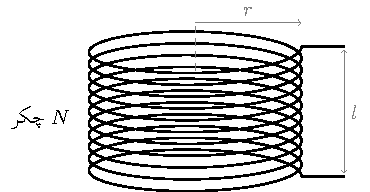
\includegraphics{figMagneticCircuitsCoil}
\caption{پیچدار لچھا}
\label{شکل_مقناطیسی_ادوار_پیچدار_لچھا}
\end{figure}
حل:
\begin{align*}
B&=\mu_0 H=\frac{\mu_0 N i}{l}\\
\phi&=B  \pi r^2=\frac{\mu_0 N i \pi r^2}{l}\\ 
\lambda&=N \phi =\frac{\mu_0 N^2 i \pi r^2}{l}\\ 
L&=\frac{\lambda}{i}=\frac{\mu_0 N^2 \pi r^2}{l}
\end{align*} 
یوں
\begin{align*}
L=\frac{4 \pi 10^{-7} \times 11^2 \times \pi  \times 0.49^2}{0.94}=\SI{122}{\micro \henry}
\end{align*}
یہ پیچدار لچھا میں نے  \عددیء{3000} کلو گرام لوہا گلانے والی بھٹی میں استعمال کیا ہے۔
\انتہا{مثال}
%
شکل \حوالہ{شکل_مقناطیسی_ادوار_دو_لچھے_ایک_درز} میں دو لچھے والا ایک مقناطیسی دور دکھایا گیا ہے۔ ایک لچھے کے  \عددیء{N_1} چکر ہیں اور اس میں برقی رو \عددیء{i_1} ہے اور دوسرا لچھا \عددیء{N_2} چکر کا ہے اور اس میں برقی  رو \عددیء{i_2} ہے۔ دونوں لچھوں میں برقی رو کی سمتیں یوں ہیں کہ اِن  دونوں کا مقناطیسی دباؤ جمع ہو۔ یوں اگر مرکز کے امالہ کو نظرانداز کیا جائے تو ہم مقناطیسی بہاؤ \عددیء{\phi} کے لئے لکھ سکتے ہیں
\begin{align}
\phi=\left (N_1 i_1 +N_2 i_2 \right ) \frac{\mu_0 A_a}{l_a}
\end{align} 
%
\begin{figure}
\centering
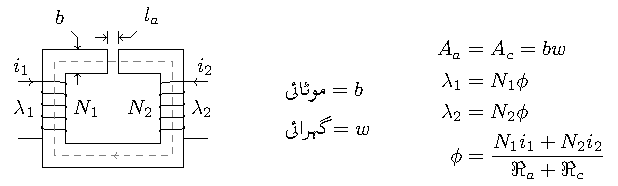
\includegraphics{figMagneticCircuitsTwoCoilsWithGap}
\caption{دو لچھے والا مقناطیسی دور۔}
\label{شکل_مقناطیسی_ادوار_دو_لچھے_ایک_درز}
\end{figure}
یہاں \عددیء{\phi} دونوں لچھوں کے مجموعی مقناطیسی دباؤ یعنی \عددیء{N_1 i_1+N_2 i_2} سے پیدا ہونے والا مقناطیسی بہاؤ ہے۔ اس مقناطیسی بہاؤ  کی ان  لچھوں  کے ساتھ  اِرتَباط کو یوں لکھا جا سکتا ہے۔
\begin{align}
\lambda_1=N_1 \phi=N_1^2  \frac{\mu_0 A_a}{l_a} i_1 +N_1 N_2  \frac{\mu_0 A_a}{l_a} i_2
\end{align}
اس کو یوں لکھا جا سکتا ہے
\begin{align}
\lambda_1 = L_{11} i_1+L_{12} i_2
\end{align}
جہاں
\begin{align}
L_{11}&=N_1^2  \frac{\mu_0 A_a}{l_a}\\
L_{12}&=N_1 N_2  \frac{\mu_0 A_a}{l_a}
\end{align}
ہیں۔ یہاں \عددیء{L_{11}} پہلے لچھے کی  خود امالہ\فرہنگ{خود امالہ}\حاشیہب{self inductance}\فرہنگ{self inductance}  ہے اور  \عددیء{L_{11} i_1} اِس لچھے کی اپنے برقی رو \عددیء{i_1} سے پیدا مقناطیسی بہاؤ  کے ساتھ  اِرتَباطِ بہاؤ ہے جسے خود اِرتَباطِ بہاؤ\فرہنگ{خود ارتباط بہاو}\حاشیہب{self flux linkage}\فرہنگ{self flux linkage} کہتے ہیں۔\عددیء{L_{12}}  اِن دونوں لچھوں  کا  مشترکہ امالہ\فرہنگ{مشترکہ امالہ}\حاشیہب{mutual inductance}\فرہنگ{mutual inductance} ہے اور  \عددیء{L_{12} i_2}  لچھا نمبر-1  کے ساتھ برقی رو  \عددیء{i_2} کی وجہ سے پیدا کردہ مقناطیسی بہاؤ  کا اِرتَباطِ بہاؤ  ہے جسے مشترکہ اِرتَباطِ بہاؤ\فرہنگ{مشترکہ ارتباط امالہ}\حاشیہب{mutual flux linkage}\فرہنگ{mutual flux linkage}  کہتے ہیں ۔ بالکل اسی طرح ہم دوسرے لچھے کے لئے لکھ سکتے ہیں
\begin{align}
\lambda_2&=N_2 \phi=N_2 N_1 \frac{\mu_0 A_a}{l_a} i_1+N_2^2 \frac{\mu_0 A_a}{l_a} i_2\\
&=L_{21} i_1+L_{22} i_2
\end{align}
جہاں
\begin{align}
L_{22}&=N_2^2 \frac{\mu_0 A_a}{l_a}\\
L_{21}&=L_{12}=N_2 N_1 \frac{\mu_0 A_a}{l_a}
\end{align}
ہیں۔\عددیء{L_{22}} دو نمبر لچھے  کی خود امالہ اور  \عددیء{L_{21}=L_{12}} ان  دو لچھوں کی مشترکہ امالہ ہے۔ یہاں یہ واضح کرنا ضروری ہے کہ امالہ کا تصور اس وقت کارآمد ہوتا جب ہم مقناطیسی مستقل \عددیء{\mu}  کو اٹل تصور کر سکیں۔

مساوات  کو مساوات  میں استعمال کریں تو 
\begin{align}
e=\frac{\partial \lambda}{\partial t}=\frac{ \partial \left (N \phi \right)}{\partial t}=\frac{\partial \left( L i\right) }{\partial t}
\end{align}
اگر امالہ مقررہ ہو جیسا کہ ساکن آلوں میں ہوتا ہے تب ہمیں  امالہ کی جانی پہچانی مساوات ملتی ہے 
\begin{align}
e=L \frac{\partial i}{\partial t}
\end{align}
مگر اگر امالہ بھی تبدیل ہو جیسا کہ موٹروں اور جنریٹروں میں ہوتا ہے تب
\begin{align}
e= L \frac{\partial i}{\partial t} + i \frac{\partial L}{\partial t}
\end{align}
توانائی\فرہنگ{توانائی}\حاشیہب{energy}\فرہنگ{energy}  کی اکائی جاؤل\فرہنگ{جاؤل}\حاشیہب{Joule}\فرہنگ{Joule} \عددیء{J}\حاشیہد{جیمس پریسقوٹ جاؤل انگلستانی سائنسدان جنہوں نے حرارت اور میکانی کام کا رشتہ دریافت کیا} ہے اور طاقت\فرہنگ{طاقت}\حاشیہب{power}\فرہنگ{power}  کی اکائی\حاشیہد{سکاٹلینڈ کے جیمز واٹ جنہوں نے بخارات پر چلنے والے انجن پر کام کیا} جاؤل فی سیکنڈ یا واٹ\فرہنگ{واٹ}\حاشیہب{Watt}\فرہنگ{Watt} \عددیء{W}  ہے۔

اس کتاب میں توانائی یا کام کو \عددیء{W} سے ظاہر کیا جائے گا مگر طاقت کی اکائی واٹ \عددیء{W} کے لئے بھی ہی کی علامت استعمال ہوتی ہے۔امید کی جاتی ہے کہ اس سے غلطی پیش نہیں آئے گی اور استعمال کو دیکھ کر یہ فیصلہ کرنا کہ اس کا کون سا مطلب لیا جا رہا ہے دشوار نہ ہوگا۔

وقت کے ساتھ توانائی کی شرح کو طاقت کہتے ہیں لہٰذا کسی لچھے کے لئے ہم لکھ سکتے ہیں
\begin{align}
p=\frac{\dif W}{\dif t} = e i = i \frac{\partial \lambda}{\partial t}
\end{align} 
لہٰذا ایک مقناطیسی دور میں  \عددیء{t_1} سے \عددیء{t_2} تک کے وقفے میں مقناطیسی توانائی میں تبدیلی کو تکمل کے ذریعہ یوں حاصل کیا جا سکتا ہے۔
\begin{align}
\Delta W = \int_{t1}^{t2} p \dif t =\int_{\lambda1}^{\lambda2} i \dif \lambda
\end{align}
اگر مقناطیسی دور میں ایک ہی لچھا ہو اور اس دور میں امالہ اٹل ہو تب
\begin{align}
\Delta W = \int_{\lambda1}^{\lambda2} i \dif \lambda=\int_{\lambda1}^{\lambda2} \frac{\lambda}{L} \dif \lambda=\frac{1}{2 L} \left(\lambda_2^2-\lambda_1^2 \right)
\end{align}

	اگر ہم لمحہ \عددیء{t_1} پہ \عددیء{\lambda_1=0} تصور کریں تب ہم کسی دیئے گئے \عددیء{\lambda} پہ مقناطیسی توانائی کو یوں لکھ سکتے ہیں
\begin{align}
\Delta W=\frac{\lambda^2}{2L}=\frac{L i^2}{2}
\end{align}

\حصہ{مقناطیسی مادہ کے خصوصیات}
مقناطیسی دوروں میں مرکز استعمال کرنے سے دو طرح کے فوائد حاصل ہوتے ہیں۔ مرکز کے استعمال سے ایک تو کم مقناطیسی دباؤ سے زیاد مقناطیسی بہاؤ پیدا کی جا سکتی ہے اور دوسری، مقناطیسی بہاؤ کو اپنی مرضی کے راستوں پابند کیا جاسکتا ہے۔ ٹرانسفارمروں میں مرکز کو استعمال کر کے مقناطیسی بہاؤ کو اِس طرح پابند کیا جاتا ہے کہ جو مقناطیسی بہاؤ ایک لچھے سے گزرتا ہے، وہی مقناطیسی بہاؤ، سارا کا سارا، باقی لچھوں سے بھی گزرتا ہے۔ موٹروں میں مرکز کو استعمال کرکے مقناطیسی بہاؤ کو یوں پابند کیا جاتا ہے کہ زیادہ سے زیادہ قوت پیدا ہو جبکہ جنریٹروں میں اسے زیادہ سے زیادہ برقی دباؤ حاصل کرنے کی نیت سے پابند کیا جاتا ہے۔
\begin{figure}
\centering
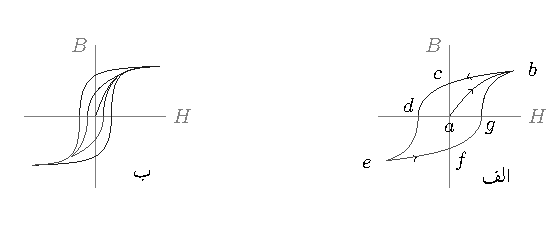
\includegraphics{figMagneticCircuitsBHSingleLoop}
\caption{$BH$   خطوط یا مقناطیسی چال کے دائرے}
\label{شکل_مقناطیسی_چال}
\end{figure}
مقناطیسی اشیاء کی \عددیء{B} اور \عددیء{H} کے تعلق کو گراف کے ذریعہ سے پیش کیا جاتا ہے۔ لوہا نما مقناطیسی اشیاء کی \عددیء{B-H}  گراف شکل \حوالہ{شکل_مقناطیسی_چال}-الف میں دکھائی گئی ہے۔ایک لوہا نما مقناطیسی شہ جس میں کسی قسم کی مقناطیسی اثر نہ ہو کو نقطہ \عددیء{a} سے ظاہر کیا گیا ہے۔اس نقطہ پر
\begin{gather}
\begin{aligned}
H_a&=0\\
B_a&=0
\end{aligned}
\end{gather}
ہیں۔

	ایسی شہ کو لچھے میں رکھ کر اس پر مقناطیسی دباؤ لاگو کی جا سکتی ہے۔ مقناطیسی میدان کی شدت \عددیء{H}  لاگو کرنے سے لوہا نما مقناطیسی شہ میں کثافتِ مقناطیسی بہاؤ  \عددیء{B} پیدا ہوگی۔میدانی شدت بڑھانے سے کثافتِ مقناطیسی بہاؤ بھی بڑھے گی۔اس عمل کو نقطہ  \عددیء{a} سے شروع ایک نوکدار خط سے دکھلایا گیا ہے۔میدانی شدت کو نقطہ \عددیء{b}  تک بڑھایا گیا ہے جہاں یہ مقداریں  \عددیء{H_b} اور \عددیء{B_b} ہیں۔

	اگر اس نقطہ تک پہنچنے کے بعد میدانی شدت کم کی جائے تو دیکھا یہ گیا ہے کہ واپسی کی خط مختلف راستہ اختیار کرتی ہے۔یوں نقطہ  \عددیء{b} سے اگر میدانی شدت کم کرتے کرتے صفر کی جائے تو لوہا نما شہ کی کثافتِ مقناطیسی بہاؤ کم ہو کر نقطہ \عددیء{c} پر آ پہنچتی ہے۔نقطہ \عددیء{b} سے نقطہ \عددیء{c} تک نوکدار خط اس عمل کو دکھلا رہی ہے۔اس نقطہ پر بیرونی میدانی شدت صفر ہے لیکن لوہا نما شہ کی کثافتِ مقناطیسی بہاؤ صفر نہیں۔یہ اب ایک مقناطیس بن گیا ہے جس کی کثافتِ مقناطیسی بہاؤ  \عددیء{B_c} ہے۔اس مقدار کو بقایا کثافتِ مقناطیسی بہاؤ\فرہنگ{کثافت مقناطیسی بہاؤ!بقایا}\حاشیہب{magnetic flux!residual}\فرہنگ{residual magnetic flux}  کہتے ہیں۔مصنوعی مقناطیس اسی طرح بنائے جاتے ہیں۔

اگر یہاں سے میدانی شدت منفی سمت میں بڑھائی جائے تو \عددیء{B} کم ہوتے ہوتے آخر کار ایک بار پھر صفر ہو جاتی ہے۔اس نقطہ کو \عددیء{d} سے ظاہر کیا گیا ہے۔مقناطیسیت ختم کرنے کے لئے درکار میدانی شدت کی مقدار  \عددیء{\abs{H_d}} کو مقناطیسیت ختم کرنے والی شدت یا خاتم شدت\فرہنگ{مقناطیس!خاتم شدت}\حاشیہب{coercivity}\فرہنگ{coercivity} کہتے ہیں۔

منفی سمت میں میدانی شدت بڑھاتے نقطہ \عددیء{e} حاصل ہوتا ہے جہاں سے منفی سمت کی میدانی شدت کی مقدار ایک بار پھر کم کی جاتی ہے۔یوں نقطہ \عددیء{f} حاصل ہوتا ہے جہاں میدانی شدت صفر ہونے کے باوجود کثافتِ مقناطیسی بہاؤ صفر نہیں۔اس نقطہ پر لوہا نما شہ اُلٹ سمت میں مقناطیس بن چکا ہے اور \عددیء{B_f} بقایا کثافتِ مقناطیسی بہاؤ ہے۔اسی طرح اس جانب مقناطیسیت ختم کرنے کی شدت \عددیء{\abs{H_g}} ہے۔

اگر لوہا نما شہ پر باری باری مثبت اور منفی  یکساں میدانی شدت کئی بار لاگو کی جائے تو اس کی \عددیء{B-H}  کی خط ایک بند دائرہ کی شکل اختیار کر لیتی ہے جسے مقناطیسی چال کا دائرہ\فرہنگ{مقناطیس!چال کا دائرہ}\حاشیہب{hysteresis loop}\فرہنگ{hysteresis loop}  کہتے ہیں۔یہی شکل کے حصہ الف میں دکھائی گئی ہے۔

حصہ الف میں نقطہ  \عددیء{a} سے نقطہ  \عددیء{b} پہنچنے کے بعد اگر میدانی شدت مزید بڑھائی جائے اور پھر مقناطیسی چال حاصل کی جائے تو شکل کے حصہ با کا بیرونی بند دائرہ ملتا ہے۔حصہ الف کی مقناطیسی چال یہاں اندرونی دائرہ سے دکھائی گئی ہے۔

شکل   کی طرح کے خطوط کی چونچوں (یعنی زیادہ سے زیادہ مقدار واضح کرنے والے نکتوں) میں سے اگر ایک خط گزاری جائے تو شکل \حوالہ{شکل_مقناطیسی_ادوار_ایم_پانچ_پتری_کا_خط}  حاصل ہوتی ہے۔یہ شکل ٹرانسفارمروں میں استعمال ہونے والی  \عددیء{0.3048}  ملی میٹر موٹی \عددیء{M5} پتری کا گراف ہے۔ اس خط میں موجود مواد جدول \حوالہ{جدول_مقناطیسی_ادوار_کثافت_بہاو_بالمقابل_شدت}  میں بھی دیا گیا ہے۔عموماً مسائل اس خط میں موجود مواد سے حل ہوتے ہیں۔دھیان رہے کہ اس خط میں \عددیء{H}  کا پیمانہ لاگ\حاشیہب{log} میں دکھایا گیا ہے۔

لوہا نما مقناطیسی اشیاء پر لاگو مقناطیسی شدت بڑھانے سے کثافتِ مقناطیسی بہاؤ بڑھنے کی شرع بتدریج کم ہوتی جاتی ہے حتیٰ کہ آخر کار یہ شرح خلاء کی شرح  \عددیء{\mu_0} رہ جاتی ہے یعنی
\begin{align}
\frac{\Delta B}{\Delta H}=\mu_0
\end{align}
اس اثر کو سیرابیت\فرہنگ{سیرابیت}\حاشیہب{saturation}\فرہنگ{saturation} کہتے ہیں۔یہ شکل \حوالہ{شکل_مقناطیسی_ادوار_ایم_پانچ_پتری_کا_خط}  میں واضح ہے۔
\begin{figure}
\centering
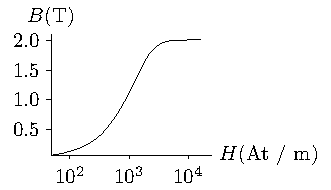
\includegraphics{figMagneticCircuitsM5curve}
\caption{$M5$ سٹیل کی $0.3048$ ملی میٹر موٹی پتری کا خط۔ میدانی شدت کا پیمانہ لاگ ہے۔}
\label{شکل_مقناطیسی_ادوار_ایم_پانچ_پتری_کا_خط}
\end{figure}
%
گراف کو دیکھا جائے تو \عددیء{B} کے کسی ایک متعین مقدار \عددیء{H} کے لئےکے دو ممکنہ مقدار ہیں۔ اگر مقناطیسی بہاؤ بڑھ رہا ہو تو، گراف میں نیچے سے اُوپر جانے والی لکیر، اِس میں \عددیء{B} اور \عددیء{H} کے تعلق کو پیش کرتی ہے اور اگر مقناطیسی بہاؤ کم ہو رہا ہو تو، اوپر سے نیچے آنے والی لکیر، اِس تعلق کو پیش کرتی ہے۔  چونکہ \عددیء{\mu=B/H} ، لہٰذا \عددیء{B} کے  مقدار تبدیل ہونے سے \عددیء{\mu} بھی تبدیل ہوتی ہے۔ باوجود اِس کے ہم مقناطیسی دوروں میں یہ تصور کرتے ہیں کہ \عددیء{\mu} ایک مقررہ ہے۔ یہ تصور کر لینے سے عموماً جواب پر زیادہ اثر نہیں پڑتا۔
%
\begin{table}
\begin{tabular}{l l l l   l l l l   l l l l}
$H$&$B$&$H$&$B$&$H$&$B$&$H$&$B$&$H$&$B$&$H$&$B$\\
\hline\\
9000&1.998&1000&1.852&           200&1.720 &30&1.480               &9&0.700&  0&0.000    \\
10000&2.000&2000&1.900&         300&1.752 &40&1.540           &10&0.835&  2&0.040    \\
20000&2.020&3000&1.936&         400&1.780 &50&1.580          &11.22&1.000&  3&0.095    \\
30000&2.040& 4000&1.952&        500&1.800 &60&1.601         &12.59&1.100 &  4&0.160    \\
40000&2.048&5000&1.968&         600&1.810 &70&1.626          &14.96&1.200&   5&0.240    \\
50000&2.060&6000&1.975&         700&1.824 &80&1.640         &17.78&1.300&  6&0.330    \\
60000&2.070&7000&1.980&         800&1.835  &90&1.655         &20&1.340&  7&0.440    \\
 70000&2.080&8000&1.985&        900&1.846 &100&1.662          &23.77&1.400& 8&0.560    \\
\hline
\end{tabular}
\caption{مقناطیسی بہاو بالمقابل شدت}
\label{جدول_مقناطیسی_ادوار_کثافت_بہاو_بالمقابل_شدت}
\end{table}
%
\ابتدا{مثال}
شکل  یا اس کے مساوی فہرست میں دیئے گئے مواد کو استعمال کرتے ہوئے شکل  کی خلاء میں ایک ٹیسلہ اور دو ٹیسلہ کثافتِ  مقناطیسی بہاؤ حاصل کرنے کے لئے درکار برقی رو معلوم کریں۔اس شکل میں
\begin{align*}
b=\SI{5}{\centi\meter},w=\SI{4}{\centi\meter},l_a=\SI{3}{\milli\meter},l_c=\SI{30}{\centi\meter},N=1000
\end{align*}
ہیں۔مرکز اور خلاء کی رقبہ عمودی تراش برابر لیں۔

حل: ایک ٹیسلہ کے لئے۔

 فہرست  سے ہم دیکھتے ہیں کہ مرکز میں \عددیء{1} ٹیسلہ  حاصل کرنے کے لئے  مرکز کو \عددیء{11.22}  ایمپیئر-چکر فی \عددیء{H} میٹر  درکار ہے۔یوں \عددیء{30} سم لمبے مرکز کو \عددیء{0.3\times 11.22=3.366}  ایمپیئر چکر درکار ہیں۔

خلاء کو
\begin{align*}
H=\frac{B}{\mu_0}=\frac{1}{4\pi 10^{-7}}=\num{795671}
\end{align*}
ایمپیئر-چکر فی میٹر درکار ہیں۔لہٰذا \عددیء{ 3 } ملی میٹر لمبی خلاء کو \عددیء{0.003 \times 795671=2387} ایمپیئر چکر درکار ہیں۔یوں کُل ایمپیئر-چکر \عددیء{3.366+2387=2390.366} ہیں جن سے 
\begin{align*}
i=\frac{2390.366}{1000}=\SI{2.39}{\ampere}
\end{align*}	
حاصل ہوتی ہے۔

حل: دو ٹیسلہ کے لئے۔

فہرست سے ہم دیکھتے ہیں کہ مرکز میں \عددیء{2} ٹیسلہ  حاصل کرنے کے لئے  مرکز کو \عددیء{10000} ایمپیئر-چکر فی میٹر \عددیء{H} درکار ہے۔یوں \عددیء{30} سم لمبے مرکز کو \عددیء{0.3 \times 10000=3000} ایمپیئر چکر درکار ہیں۔خلاء کو
\begin{align*}
H=\frac{B}{\mu_0}=\frac{2}{4\pi 10^{-7}}=\num{1591342}
\end{align*}
ایمپیئر-چکر فی میٹر درکار ہیں۔لہٰذا \عددیء{3} ملی میٹر لمبی خلاء کو  \عددیء{0.003 \times 1591342=4774}  ایمپیئر چکر درکار ہیں۔یوں کُل ایمپیئر-چکر \عددیء{3000+4774=7774}	ہیں جن سے 
\begin{align*}
i=\frac{7774}{1000}=\SI{7.774}{\ampere}
\end{align*}
حاصل ہوتی ہے۔

اس مثال میں مقناطیسی سیرابیت کے اثرات واضح ہیں۔ 
\انتہا{مثال}
%
\حصہ{ہیجان شدہ لچھا}
بدلتی رو میں برقی دباؤ اور مقناطیسی بہاؤ سائن نما ہوتے ہیں یعنی یہ وقت کے ساتھ \عددیء{\sin \omega t} یا \عددیء{\cos \omega t} کا تعلق رکھتے ہیں۔ اِس سبق میں ہم بدلتی رو سے لچھے کو ہیجان کرنا اور اس سے نمودار ہونے والے برقی توانائی  کے ضیاع  کا تذکرہ  کریں گے۔ شکل  سے رجوع کریں۔ ہم فرض کرتے ہیں کہ مرکز میں کثافتِ مقناطیسی بہاؤ 
\begin{align}
B=B_0 \sin \omega t
\end{align}
یوں مرکز میں بدلتا مقناطیسی بہاؤ \عددیء{\varphi}
\begin{align}
\varphi=A_c B=A_c B_0 \sin \omega t=\phi_0 \sin \omega t
\end{align}
ہے۔اس مساوات میں مقناطیسی بہاؤ کا حیطہ  \عددیء{\mp\phi_0} اور \عددیء{B} کا حیطہ \عددیء{\mp B_0} کے مابین تبدیل ہوتے ہیں۔\عددیء{A_c} مرکز کا رقبہ عمودی تراش ہے جو ہر جگہ یکساں ہے ۔\عددیء{\omega = 2 \pi f} ہے جہاں \عددیء{f} تعدد ہے۔

فیراڈے کے قانون یعنی مساوات  کے تحت اس مقناطیسی بہاؤ کی وجہ سے لچھے میں \عددیء{e(t)} برقی دباؤ  پیدا ہو گی۔
\begin{gather}
\begin{aligned}
e(t)&=\frac{\partial \lambda}{\partial t}\\
&=\omega N \phi_0 \cos \omega t \\
&=\omega N A_c B_0 \cos \omega t\\
&=E_0 \cos \omega t
\end{aligned}
\end{gather}
جس کا حیطہ
\begin{align}
E_0=\omega N \phi_0=2 \pi f N A_c B_0
\end{align}
ہے۔\عددیء{e(t)} کو امالی برقی دباؤ\فرہنگ{امالی برقی دباؤ}\حاشیہب{induced voltage}\فرہنگ{induced voltage} کہتے ہیں۔ 

ہم بدلتی رو مقداروں کے مربع کی اوسط کے جزر  میں دلچسپی رکھتے ہیں۔یہی ان مقداروں کی موثر\فرہنگ{موثر}\حاشیہب{root mean square, rms}\فرہنگ{rms} قیمت ہوتی ہے۔ جیسا مساوات  میں دیکھا گیا ہے، ایک سائن نما  موج کی موثر قیمت اس کے حیطہ کے  \عددیء{1/\sqrt{2}} گنّا ہوتی ہے لہٰذا 
\begin{align}
E_{rms}=\frac{E_0}{\sqrt{2}}=\frac{2 \pi f N A_c B_0}{\sqrt{2}}=4.44 f N A_c B_0
\end{align}
یہ مساوات بہت اہمیت رکھتی ہے اور ہم اس کو بار بار استعمال کریں گے۔بدلتی برقی دباؤ یا بدلتی برقی رو کی مقدار کی جب بھی ذکر ہو، یہ ان کی مربع کی اوسط کے جزر  یعنی اس کے موثر قیمت  کا ذکر ہوتا ہے۔پاکستان میں گھریلو برقی دباؤ \عددیء{220} وولٹ ہے۔اس کا مطلب ہے کہ اس برقی دباؤ کی موثر قیمت \عددیء{220} وولٹ ہے۔ چونکہ یہ سائن نما ہے لہٰذا اس کی چوٹی \عددی{\sqrt{2} \times 220=311} وولٹ ہے۔
%
\ابتدا{مثال}
شکل میں \عددیء{27} چکر ہیں۔ مرکز کی لمبائی \عددیء{30 } سم جبکہ اس کا رقبہ عمودی تراش \عددیء{229.253} مربع سم ہے۔لچھے  میں گھریلو \عددیء{220} وولٹ موثر برقی دباؤ سے ہیجان  پیدا کیا جاتا ہے۔فہرست کی مدد سے مختلف برقی دباؤ پر محرک برقی رو معلوم کریں اور اس کا گراف بنائیں۔

حل:
	گھریلو برقی دباؤ \عددیء{50} ہرٹز کی سائن نما موج ہوتی ہے یعنی
\begin{align}
v=\sqrt{2} \times 220 \cos (2 \pi  50 t)
\end{align}
مساوات  کی مدد سے ہم کثافتِ مقناطیسی بہاؤ کی چوٹی حاصل کرتے ہیں
\begin{align}
B_0=\frac{220}{4.44 \times 50 \times 27 \times 0.0229253}=\SI{1.601}{\tesla}
\end{align}
لہٰذا مرکز میں کثافتِ مقناطیسی بہاؤ صفر سے \عددیء{\mp1.601}  ٹیسلہ کے درمیان تبدیل ہوتی رہتی ہے۔یوں مرکز میں کثافتِ مقناطیسی بہاؤ کی مساوات یہ ہو گی
\begin{align}
B=1.601 \sin \omega t
\end{align}
ہم فہرست کی مدد سے کثافتِ مقناطیسی بہاؤ کے  \عددی{0} سے \عددیء{1.601} ٹیسلہ کے درمیان مختلف قیمتوں پر درکار محرک برقی رو \عددیء{i_{\phi}} معلوم کرنا چاہتے ہیں۔ہم مختلف \عددیء{B} پر فہرست سے مرکز کی \عددیء{H} حاصل کریں گے جو کہ ایک میٹر لمبی مرکز کے لئے درکار ایمپیئر-چکر دیتی ہے۔اس سے \عددیء{30} سم لمبی مرکز کے لئے درکار ایمپیئر-چکر  حل کر کے برقی رو حاصل کریں گے۔

%
\begin{table}
\begin{tabular}{l l l l l | l l l l l}
$i_{\varphi}=\frac{0.3 H}{27}$&$0.3H$&$H$&$B$&$\omega t$&$i_{\varphi}=\frac{0.3 H}{27}$&$0.3H$&$H$&$B$&$\omega t$\\
\hline\\
0.000&0.000&0&0.000&0.000&0.125&3.366&11.22&1.000&0.675\\
0.022&0.600&2&0.040&0.025&0.140&3.777&12.59&1.100&0.757\\
0.033&0.900&3&0.095&0.059&0.166&4.488&14.96&1.200&0.847\\
0.044&1.200&4&0.160&0.100&0.198&5.334&17.78&1.300&0.948\\
0.056&1.500&5&0.240&0.150&0.222&6.000&20&1.340&0.992\\
0.067&1.800&6&0.330&0.208&0.264&7.131&23.77&1.400&1.064\\
0.078&2.100&7&0.440&0.278&0.333&9.000&30&1.480&1.180\\
0.089&2.400&8&0.560&0.357&0.444&12.000&40&1.540&1.294\\
0.100&2.700&9&0.700&0.453&0.556&15.000&50&1.580&1.409\\
0.111&3.000&10&0.835&0.549&0.667&18.000&60&1.601&1.571\\
\hline
\end{tabular}
\caption{محرک برقی رو}
\label{جدول_مقناطیسی_ادوار_محرک_برقی_رو_بالمقابل_کثافت_بہاو}
\end{table}


جدول \حوالہ{جدول_مقناطیسی_ادوار_محرک_برقی_رو_بالمقابل_کثافت_بہاو}  مختلف کثافتِ مقناطیسی بہاؤ کے لئے درکار محرک برقی رو دیتی ہے۔جدول میں  ہر \عددیء{B} کی قیمت پر  \عددیء{\omega t} مساوات  کی مدد سے حاصل کی گئی ہے۔\عددیء{\omega t} بالمقابل محرک برقی رو کا گراف شکل \حوالہ{شکل_مقناطیسی_ادوار_ہیجان_رو_چال_نظرانداز} میں دیا گیا ہے۔
\انتہا{مثال}
%
\begin{figure}
\centering
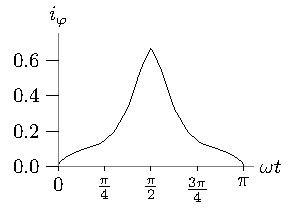
\includegraphics{figMagneticCircuitsExcitationCurrentNeglectingHysterisys}
\caption{$M5$ پتری کے مرکز میں $1.6$ ٹیسلہ تک ہیجان پیدا کرنے کے لئے درکار ہیجان انگیز برقی رو۔}
\label{شکل_مقناطیسی_ادوار_ہیجان_رو_چال_نظرانداز}
\end{figure}
برقی لچھے میں برقی دباؤ سے ہیجان پیدا کیا جاتا ہے۔ہیجان شدہ لچھے میں برقی رو کی وجہ سے  مرکز میں مقناطیسی بہاؤ پیدا ہوتا ہے۔ اس برقی رو \عددیء{i_{\phi}} کو ہم ہیجان انگیز برقی رو\فرہنگ{برقی رو!ہیجان انگیز}\حاشیہب{excitation current}\فرہنگ{excitation current}  کہتے ہیں۔

مثال میں ہیجان انگیز برقی رو معلوم کی گئی جسے شکل \حوالہ{شکل_مقناطیسی_ادوار_ہیجان_رو_چال_نظرانداز} میں دکھایا گیا۔اسے حاصل کرتے وقت مقناطیسی چال\فرہنگ{مقناطیسی چال}\حاشیہب{hysteresis} کو نظر انداز کیا گیا۔شکل \حوالہ{شکل_مقناطیسی_ادوار_ہیجان_رو_بشمول_اثر_چال} میں ہیجان انگیز برقی رو دکھائی گئی ہے جو مقناطیسی چال کو مدِ نظر رکھ کر حاصل کی گئی ہے۔ اس کو سمجھنا نہایت ضروری ہے۔
\begin{figure}
\centering
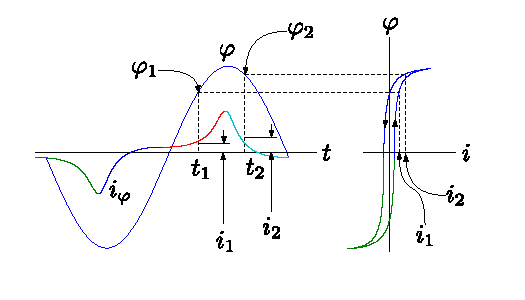
\includegraphics{figExcitationCurrentFromBHbrillouinCurve}
\caption{ہیجان انگیز برقی رو۔}
\label{شکل_مقناطیسی_ادوار_ہیجان_رو_بشمول_اثر_چال}
\end{figure}
اس شکل  میں دائیں جانب مقناطیسی چال کی خط ہے۔ چونکہ 
\begin{gather}
\begin{aligned}
H l& =N i\\
\varphi&=B A_c
\end{aligned}
\end{gather}
لہٰذا اس خط کو \عددیء{\varphi-i_{\varphi}} کا خط تصور کیا جا سکتا ہے۔شکل کی بائیں جانب مرکز میں سائن نما مقناطیسی بہاؤ \عددیء{\varphi} دکھائی گئی ہے۔یہ سائن نما مقناطیسی بہاؤ کی موج وقت کے ساتھ تبدیل ہوتی ہے۔لمحہ \عددیء{t_1} پر اس موج کی مقدار  \عددیء{\varphi_1} ہو گی۔ یہ شکل میں دکھائی گئی ہے۔اتنی مقناطیسی بہاؤ حاصل کرنے کے لئے درکار ہیجان انگیز برقی رو \عددیء{i_{\varphi1}} مقناطیسی چال کی خط سے حاصل کی جا سکتی ہے۔اس  ہیجان انگیز برقی رو کو شکل میں لمحہ \عددیء{t_1} پر دکھایا گیا ہے۔ 

دھیان رہے کہ اس لمحہ مقناطیسی بہاؤ بڑھ رہی ہے لہٰذا مقناطیسی چال کی خط کا صحیح حصہ استعمال کرنا ضروری ہے۔ شکل  میں اس حصہ  کو \عددیء{efgb} سے واضح کیا گیا ہے۔

اسی طرح ایک اور لمحہ \عددیء{t_2} جب مقناطیسی بہاؤ کم ہو رہی ہے یہی کچھ دوبارہ شکل میں ہوتے دکھایا گیا ہے البتہ اس مرتبہ شکل میں \عددیء{bcde} سے واضح کیا گیا حصہ استعمال کیا گیا ہے۔اس لمحہ پر مقناطیسی بہاؤ \عددیء{\varphi_2} ہے اور اسے حاصل کرنے کے لئے درکار ہیجان انگیز برقی رو \عددیء{i_{\varphi2}} ہے۔

اگر اسی طرح مختلف لمحات پر درکار ہیجان انگیز برقی رو حاصل کی جائے تو ہمیں شکل میں دکھائی گئی  \عددیء{i_{\varphi}} کی خط ملے گی۔یہ ایک غیر سائن نما خط ہے۔

 اگر مرکز میں  \عددیء{B=B_0 \sin \omega t} ہو  تو اِس میں \عددیء{H} اور \عددیء{i_{\varphi}} ایک غیر سائن نما شکل اختیار کر لیتے ہیں۔ اس صورت میں  اِن کے موثر قیمتوں \عددیء{H_{c,rms}} اور  \عددیء{i_{\varphi,rms}} کا تعلق یہ ہے
\begin{align}
N i_{\varphi,rms}=l_c H_{c,rms}
\end{align}
مساوات   اور  سے ملتا ہے
\begin{align}
E_{rms} i_{\varphi,rms}=\sqrt{2} \pi f B_0 H_{c,rms} A_c l_c
\end{align}
یہاں \عددیء{A_c l_c} مرکز کا حجم ہے۔ لہٰذا یہ مساوات ہمیں \عددیء{A_c l_c} حجم کی مرکز  کو \عددیء{B_0} کثافتِ مقناطیسی بہاؤ تک ہیجان کرنے کے لئے درکار \عددیء{E_{rms} i_{\varphi,rms}} بتلاتا ہے۔ ایک مقناطیسی مرکز جس کا حجم  \عددیء{A_c l_c} اور  میکانی کثافت  \عددیء{\rho_c} ہو، اس کی کمیت \عددیء{m_c=\rho_c A_c l_c} ہو گی۔ یوں ہم، ایک کلوگرام  مرکز، کے لئے مساوات   کو یوں لکھ سکتے ہیں
\begin{align}
P_a=\frac{E_{rms} i_{\varphi,rms}}{m_c}=\frac{\sqrt{2} \pi f}{\rho_c} B_0 H_{c,rms}
\end{align}
دیکھا جائے تو کسی ایک تعدد  \عددیء{f} پہ \عددیء{P_a} کی قیمت صرف مرکز اور اس میں \عددیء{B_0} پر منحصر ہے، چونکہ \عددیء{H_{c,rms}} خود \عددیء{B_0} پر منحصر ہے۔ اِسی وجہ سے مرکز بنانے والے، اکائی کمیت کے مرکز میں مختلف \عددیء{B_0} پیدا کرنے کیلئے درکار \عددیء{E_{rms} i_{\varphi,rms}}، کو \عددیء{B_0} اور \عددیء{P_a} کے مابین گراف کی شکل میں دیتے ہیں۔ ایسا ہی ایک گراف شکل میں دکھایا گیا ہے۔

%\باب{ٹرانسفارمر}
ٹرانسفارمر وہ آلہ ہے جو بدلتی برقی دباؤ تبدیل کرتا ہے۔ یہ دو یا دو سے زیادہ لچھوں پر مشتمل ہوتا ہے جو مقناطیسی مرکز\فرہنگ{مقناطیسی مرکز}\حاشیہب{magnetic core}\فرہنگ{core} پر لپٹے ہوتے ہیں۔یہ لچھے عموماً آپس میں جُڑے ہوئے نہیں ہوتے۔شکل \حوالہ{شکل_ٹرانسفارمر_علامت}-الف میں ٹرانسفارمر کی علامت دکھائی گئی ہے۔دو لچھوں کے درمیان متوازی لکیریں مقناطیسی مرکز کو ظاہر کرتی ہیں۔

دستیاب برقی دباؤ\حاشیہد{بدلتی برقی دباؤ کی علامت میں مثبت اور منفی نشان وقت صفر پر برقی دباؤ کی مثبت اور منفی سِرے ظاہر کرتے ہیں۔} پر ٹرانسفارمر کے ایک لچھے کو برقی طاقت فراہم کی جاتی ہے اور باقی لچھوں سے  مختلف برقی دباؤ پر یہی برقی طاقت حاصل کی جاتی ہے۔جس لچھے پر برقی دباؤ لاگو کیا جائے اسے ابتدائی لچھا\فرہنگ{لچھا!ابتدائی}\فرہنگ{ابتدائی!لچھا}\حاشیہب{primary coil}\فرہنگ{coil!primary}  کہتے ہیں اور ٹرانسفارمر کی اس جانب کو ابتدائی جانب\فرہنگ{ابتدائی!جانب}\حاشیہب{primary side}\فرہنگ{primary!side} کہتے ہیں۔اسی طرح جس لچھے (لچھوں) سے برقی طاقت حاصل کی جاتی ہے اسے (انہیں) ثانوی لچھا\فرہنگ{لچھا!ثانوی}\حاشیہب{secondary coil}\فرہنگ{coil!secondary}  (لچھے) کہتے ہیں اور اس جانب کو ثانوی جانب\فرہنگ{ثانوی جانب}\فرہنگ{side!secondary}\حاشیہب{secondary side}  کہتے ہیں۔یہ شکل کے حصہ با میں دکھایا گیا ہے۔ٹرانسفارمر کی ابتدائی جانب کو بائیں ہاتھ اور ثانوی جانب کو دائیں ہاتھ بنایا جاتا ہے۔
\begin{figure}
\centering
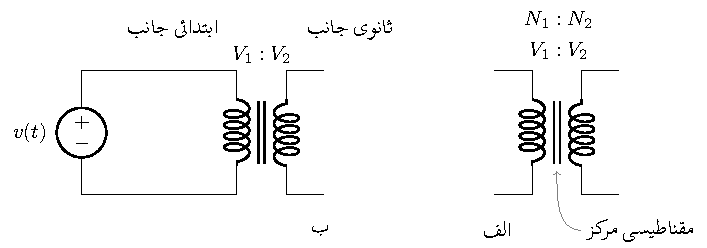
\includegraphics{figTransformersSymbol}
\caption{ٹرانسفارمر کی علامت۔}
\label{شکل_ٹرانسفارمر_علامت}
\end{figure}

بڑے ٹرانسفارمر عموما ً دو ہی لچھوں پر مشتمل ہوتے ہیں۔اس کتاب میں ہم دو ہی لچھوں کے مقناطیسی مرکز پر لپٹے قوی ٹرانسفارمر پر تبصرہ کریں گے۔

	ٹرانسفارمر کے کم برقی دباؤ کے لچھے کو کم برقی دباؤ کا لچھا\فرہنگ{لچھا!کم برقی دباؤ}\حاشیہب{low voltage coil}\فرہنگ{coil!low voltage}  کہتے ہیں اور ٹرانسفارمر کی اس جانب کو کم برقی دباؤ والی جانب  کہتے ہیں جبکہ اس کے زیادہ برقی دباؤ کے لچھے کو زیادہ برقی دباؤ کا لچھا\فرہنگ{لچھا!زیادہ برقی دباؤ}\حاشیہب{high voltage coil}\فرہنگ{coil!high voltage}  کہتے ہیں اور ٹرانسفارمر کی اس جانب کو زیادہ برقی دباؤ والی جانب  کہتے ہیں۔

یوں اگر ٹرانسفارمر کے کم برقی دباؤ کی جانب برقی دباؤ لاگو کیا جائے اور زیادہ برقی دباؤ کی جانب سے برقی دباؤ حاصل کیا جائے تو ٹرانسفارمر کی کم برقی دباؤ والی جانب کو ابتدائی جانب کہیں گے اور اس کی زیادہ برقی دباؤ والی جانب کو ثانوی جانب کہیں گے۔

\حصہ{ٹرانسفارمر کی اہمیت}
بدلتی رو کی برقی طاقت اتنی مقبول اس لئے ہوئی ہے کہ یہ ایک جگہ سے دوسری جگہ با آسانی اور نہایت کم برقی طاقت کی ضیاع کے ساتھ منتقل کی جا سکتی ہے۔ٹرانسفارمر کی تبادلہ برقی دباؤ\فرہنگ{برقی دباؤ!تبادلہ}\حاشیہب{voltage transformation property} کی خصوصیت ایسا کرنے میں کلیدی کردار ادا کرتی ہے۔ یہ ایک مثال سے بہتر سمجھا جا سکتا ہے۔
%
\ابتدا{مثال}
شکل \حوالہ{شکل_ٹرانسفارمر_برقی_طاقت_منتقلی}  سے رجوع کریں۔برقی دباؤ اور برقی رو کی حاصلِ ضرب برقی طاقت ہوتی ہے یعنی
\begin{figure}
\centering
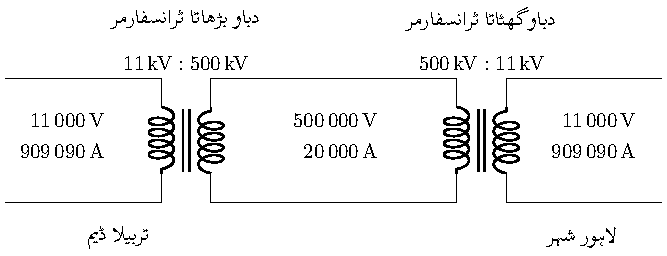
\includegraphics{figTransformersVoltageStepUpBenefits}
\caption{برقی طاقت کی منتقلی۔}
\label{شکل_ٹرانسفارمر_برقی_طاقت_منتقلی}
\end{figure}

%
\begin{align*}
p=v_1 i_1 = v_2 i_2
\end{align*}
اب تصور کریں کہ تربیلا ڈیم \عددیء{10,000,000,000} واٹ یعنی دس گیگا واٹ\حاشیہب{Giga Watt}  برقی طاقت پیدا کر رہا ہے اور اس طاقت کو لاہور\حاشیہد{ضلع صوابی میں بھی لاہور ایک تحصیل ہے لیکن اس شہر کو اتنی طاقت نہیں درکار } شہر منتقل کرنا ہے جہاں گھریلو صارفین کو یہ \عددیء{220} وولٹ پر مہیا کرنی ہے۔اگر ہم اس طاقت کو \عددیء{220}  وولٹ پر ہی منتقل کرنا چاہیں تو برقی رو
\begin{align*}
i=\frac{p}{v}=\frac{\num{10000000000}}{220}=\SI{45454545}{\ampere}
\end{align*}
ہو گی۔برقی تار میں کثافتِ برقی رو \عددیء{J_{au}} تقریباً \عددیء{5} ایمپیئر فی مربہ ملی میٹر \عددیء{J_{au}=\SI{5}{\ampere \per \milli\meter \squared}}  ممکن ہوتی ہے۔یہ ایک محفوظ کثافتِ برقی رو ہے۔اگر برقی تار میں اس سے زیادہ برقی رو گزاری جائے تو اس کی مزاحمت میں برقی طاقت کے ضیاع سے یہ گرم ہو کر پگل سکتی ہے۔ اس طرح مساوات سے برقی تار کا رقبہ عمودی تراش
\begin{align*}
A=\frac{i}{J_{au}}=\frac{45454545}{5}=\SI{9090909}{\milli\meter\squared}
\end{align*}
ہو گا۔ گول تار تصور کریں تو اس کا رداس
\begin{align*}
r=\sqrt{\frac{A}{\pi}}=\sqrt{\frac{9090909}{\pi}}=\SI{1701}{\milli\meter}=\SI{1.7}{\meter}
\end{align*}
حاصل ہوتی ہے۔آپ نے دیکھا کہ درکار برقی تار کا رداس \عددیء{1.7} میٹر ہے۔اتنی موٹی برقی تار کہیں نہیں پائی جاتی ہے\حاشیہد{آپ مانیں یا نہ مانیں، آپ نے بھی اتنی موٹی برقی تار کبھی نہیں دیکھی}۔اگر یہ تار المونیم کی بنی ہو جس کی  کثافت  \عددیء{\rho_v=\SI{2700}{\kilo\gram\per\meter\squared}} ہے تو ایک میٹر لمبی تار کی کمیت
\begin{align*}
m=2700 \times \pi \times 1.7^2 \times 1=\SI{24513}{\kilo\gram}
\end{align*}
یعنی \عددیء{24} ٹن ہوگی۔المونیم اتنی مہنگی ہے کہ اس صورت میں اتنی برقی طاقت کو لاہور پہنچانا ممکن نہیں\حاشیہد{آج کل لاہور میں لوڈ شیدنگ اس وجہ سے نہیں}۔

ڈیم پر ایک ٹرانسفارمر نسب کیا جائے جو برقی دباؤ کو بڑھا کر  \عددیء{\num{500000}} وولٹ یعنی \عددیء{500} کلو وولٹ  کر دے تب صرف 
\begin{align*}
i=\frac{p}{v}=\frac{\num{10000000000}}{\num{500000}}=\SI{20000}{\ampere}
\end{align*}
ایمپیئر درکار ہوں گے جس کے لئے درکار برقی تار
\begin{align*}
A&=\frac{i}{J_{au}}=\frac{\num{20000}}{5}=\SI{4000}{\milli\meter\squared}\\
r&=\sqrt{\frac{A}{\pi}}=\sqrt{\frac{4000}{\pi}}=\SI{35.7}{\milli\meter}
\end{align*}
صرف \عددیء{35} ملی میٹر رداس کی ہو گی۔
\انتہا{مثال}
%

اس مثال میں اگر تربیلا ڈیم میں نسب جنریٹر \عددیء{11000} وولٹ برقی دباؤ پیدا کر رہا ہو تو تربیلا ڈیم  پر نسب  ٹرانسفارمر برقی دباؤ کو \عددیء{11000} وولٹ سے بڑھا کر \عددیء{500} کلو وولٹ کرے گا جبکہ لاہور شہر میں نسب  ٹرانسفارمر اس برقی دباؤ کو \عددیء{500} کلو وولٹ سے واپس \عددیء{11000} وولٹ کر دے گا۔

اسی مثال کو مزید آگے لے جاتے ہیں۔شہر میں \عددیء{220} وولٹ کی بجائے \عددیء{11000} وولٹ صارف تک پہنچائے جائیں گے اور۔وہیں نزدیک ایک اور ٹرانسفارمر  \عددیء{11000}  وولٹ کو مزید گھٹا کر صارف کو  \عددیء{220} وولٹ فراہم کرے گی۔ 

شکل میں ڈیم سے شہر تک کا نظام دکھایا گیا ہے جہاں ڈیم پر نسب ٹرانسفارمر کو برقی دباؤ بڑھاتا ٹرانسفارمر\فرہنگ{ٹرانسفارمر!دباؤ بڑھاتا}\حاشیہب{step up transformer}\فرہنگ{step up transformer}  اور لاہور میں نسب ٹرانسفارمر کو برقی دباؤ گھٹاتا ٹرانسفارمر\فرہنگ{ٹرانسفارمر!دباؤ گھٹاتا}\حاشیہب{step down transformer}\فرہنگ{step down transformer}  کہا گیا ہے۔

موجودہ دور میں برقی طاقت \عددیء{11} کلو وولٹ اور  \عددیء{25} کلو وولٹ کے مابین پیدا کی جاتی ہے۔اس کی منتقلی  \عددیء{110 } کلو وولٹ اور \عددیء{1000}  کلو وولٹ کے مابین کی جاتی ہے جبکہ اس کا استعمال  \عددیء{1000} وولٹ سے کم پر کیا جاتا ہے۔

\حصہ{3.2 ٹرانسفارمر کے اقسام}
گھروں اور کارخانوں کو برقی طاقت فراہم کرنے والے ٹرانسفارمر مقناطیسی مرکز پر لپٹے جاتے ہیں۔یہ عموما ً تین دور کے لئے لپٹے جاتے ہیں اور انہیں لوہے کے مرکز والے تین دور کے قوی ٹرانسفارمر\حاشیہب{iron core, three phase power transformer} کہتے ہیں۔

نہایت چھوٹے ٹرانسفارمر عموماً لوہے کی مرکز والے ایک دور کے ہوتے ہیں۔یہ گھریلو استعمال کے برقی مشین، مثلاً موبائل چارجر، میں لگے ہوتے ہیں اور \عددیء{220} وولٹ سے برقی دباؤ مزید گھٹاتے ہیں۔

کچھ ٹرانسفارمر اس طرح بنائے جاتے ہیں کہ ان کی ثانوی جانب برقی دباؤ ان کی ابتدائی جانب برقی دباؤ کی خاص نسبت سے ہو۔یہ نسبت حاصل کرنے پر خاص توجہ دی جاتی ہے۔ انہیں میٹر والے دباؤ کے ٹرانسفارمر\فرہنگ{ٹرانسفارمر!برقی دباؤ، میٹر}\حاشیہب{potential transformer}  کہتے ہیں۔اسی طرح کچھ ٹرانسفارمر اس طرح بنائے جاتے ہیں کہ ان کی ثانوی جانب برقی رو، ابتدائی جانب برقی رو کی خاص نسبت سے ہو۔ یہ نسبت حاصل کرنے پر خاص توجہ دی جاتی ہے۔ان کو میٹر والے رو کے ٹرانسفارمر\فرہنگ{ٹرانسفارمر!رو، میٹر}\حاشیہب{current transformer}  کہتے ہیں۔یہ دو قسم کے ٹرانسفارمر برقی دباؤ اور برقی رو ناپنے کے لئے استعمال ہوتے ہیں۔ ویسے تو ہر ٹرانسفارمر کسی نسبت سے ہی برقی دباؤ یا برقی رو کم یا زیادہ کرتا ہے لیکن جیسا پہلے ذکر ہوا ان دو قسم کے ٹرانسفارمروں میں کم اور زیادہ کرنے کی نسبت پر خاص توجہ رکھی جاتی ہے۔ان دو اقسام کے ٹرانسفارمروں کی برقی اہلیت\فرہنگ{برقی اہلیت}\حاشیہب{electrical rating}\فرہنگ{electrical rating} نہایت کم\حاشیہد{یہ عموما ً تقریباً پچیس وولٹ-ایمپیئر اہلیت کے ہوتے ہیں} ہوتی ہے۔

ٹرانسفارمر کے لچھوں کے مابین مشترکہ مقناطیسی بہاؤ خلاء کے ذریعہ بھی ممکن ہے۔انہیں خلائی مرکز کے ٹرانسفارمر\فرہنگ{ٹرانسفارمر!خلائی مرکز والا}\حاشیہب{air core transformer}\فرہنگ{transformer!air core}  کہتے ہیں۔ ایسے ٹرانسفارمر ذرائع ابلاغ\فرہنگ{ٹرانسفارمر!ذرائع ابلاغ}\حاشیہب{communication transformer}\فرہنگ{transformer!communication} کے ادوار، یعنی ریڈیو، ٹی وی وغیرہ میں پائے جاتے ہیں۔ان ٹرانسفارمروں کی علامت  شکل  الف کی طرح ہوتی ہے مگر اس میں مقناطیسی مرکز ظاہر کرنے والی متوازی لکیریں نہیں ہوتیں۔

\حصہ{امالی برقی دباؤ}
اس حصے کا بنیادی مقصد بیرونی برقی دباؤ \عددیء{v}  اور اندرونی امالی برقی دباؤ  \عددیء{e} میں فرق واضح کرنا اور اس سے تعلق رکھنے والی تکنیکی اصطلاح کا تعارف کرانا ہے۔

شکل  \حوالہ{شکل_ٹرانسفارمر_بیرونی_اور_اندرونی_برقی_دباو} میں ایک بے بار\فرہنگ{بے بار}\حاشیہب{unloaded} ٹرانسفارمر دکھایا گیا ہے یعنی اس کے ثانوی لچھے کو کھلے دور رکھا گیا ہے۔ابتدائی لچھے پر \عددیء{v_1} برقی دباؤ لاگو کرنے سے ابتدائی لچھے میں ہیجان انگیز\فرہنگ{ہیجان انگیز برقی رو}\حاشیہب{excitation current}\فرہنگ{excitation current} برقی رو \عددیء{i_{\varphi}} گزرے گی۔اس ہیجان انگیز برقی رو سے پیدا مقناطیسی دباؤ \عددیء{N_1 i_{\varphi}}  مرکز میں مقناطیسی بہاؤ  \عددیء{\varphi} کو جنم دے گی۔ یہ بدلتی مقناطیسی بہاؤ ابتدائی لچھے میں امالی برقی  دباؤ \عددیء{e_1}  پیدا کرتی ہے جہاں
\begin{align}
e_1=-\frac{\dif \lambda}{\dif t}=-N_1 \frac{\dif \varphi}{\dif t}
\end{align}

 اس مساوات میں
\begin{itemize}
\item
\عددیء{\lambda} ابتدائی لچھے کی مقناطیسی بہاؤ کے ساتھ اِرتَباطِ بہاؤ ہے
\item
\عددیء{\varphi} مقناطیسی مرکز میں مقناطیسی بہاؤ جو دونوں لچھوں میں سے گزرتی ہے
\item
\عددیء{N_1} ابتدائی لچھے کے چکر
\end{itemize}
%
\begin{figure}
\centering
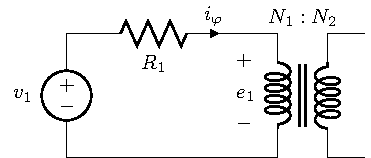
\includegraphics{figTransformersAppliedAndInducedVoltages}
\caption{بیرونی برقی دباؤ اور اندرونی امالی برقی دباؤ میں فرق۔}
\label{شکل_ٹرانسفارمر_بیرونی_اور_اندرونی_برقی_دباو}
\end{figure}

اگر اس ابتدائی لچھے کی برقی تار کی مزاحمت \عددیء{R_1} ہو تب کرچاف کے قانون برائے برقی دباؤ سے
\begin{align}\label{مساوات_ٹرانسفارمر_بیرونی_اندرونی_دباؤ_فرق}
v_1 = i_{\varphi} R_1+e_1
\end{align}

شکل میں اس مزاحمت کو ٹرانسفارمر کے باہر دکھایا گیا ہے۔اس لچھے کی رِستا متعاملہ بھی ہوتی ہے لیکن اسے یہاں نظرانداز کیا گیا ہے۔عام تر طاقت کے ٹرانسفارمر اور موٹروں  میں مزاحمت \عددیء{R_1} کے اثر کو بھی نظرانداز کیا جاسکتا ہے۔ ایسا کرنے سے ہم لکھ سکتے ہیں 
\begin{align}\label{مساوات_ٹرانسفارمر_بیرونی_اندرونی_دباؤ_تقریبا_برابر}
v_1 = e_1=-N_1 \frac{\dif \varphi}{\dif t}
\end{align}

مساوات \حوالہ{مساوات_ٹرانسفارمر_بیرونی_اندرونی_دباؤ_فرق} سے یہ ثابت ہوتا ہے کہ بیرونی لاگو برقی دباؤ اور اندرونی امالی برقی دباؤ دو علیحدہ برقی دباؤ ہیں۔یہ بات سمجھ لینا بہت ضروری ہے۔مساوات \حوالہ{مساوات_ٹرانسفارمر_بیرونی_اندرونی_دباؤ_تقریبا_برابر} کے تحت ان دو برقی دباؤ کی مقداریں عموماً برابر ہوتی ہیں۔اس کتاب میں عموماً مساوات \حوالہ{مساوات_ٹرانسفارمر_بیرونی_اندرونی_دباؤ_تقریبا_برابر}  کی طرح مساواتوں میں دائیں جانب منفی کی علامت نہیں لکھی گئی ۔عموماً برقی دباؤ کی قیمت درکار ہوتی ہے نا کہ اس کی علامت۔\حاشیہد{جس سے طلبا کو یہ غلط فہمی لاحق ہو جاتی ہے کہ یہ ایک ہی برقی دباؤ کے دو نام ہیں}

لچھا ہیجان\فرہنگ{ہیجان}\حاشیہب{excitation}\فرہنگ{excitation} کرنے سے مراد اس پر بیرونی برقی دباؤ لاگو کرنا  جبکہ لچھے پر لاگو بیرونی برقی دباؤ کو ہیجان انگیز برقی دباؤ\فرہنگ{ہیجان انگیز!برقی دباؤ}\حاشیہب{excitation voltage}\فرہنگ{excitation voltage}  کہتے ہیں۔لچھے  کو ہیجان شدہ لچھا\فرہنگ{ہیجان!لچھا}\حاشیہب{excited coil}\فرہنگ{excited coil} جبکہ اس میں رواں برقی رو کو ہیجان انگیز برقی رو\فرہنگ{ہیجان انگیز!برقی رو}\فرہنگ{excitation current}\حاشیہب{excitation current} کہتے ہیں۔

برقی دباؤ عموماً لچھے سے گزرتی مقناطیسی بہاؤ کی تبدیلی سے حاصل کی جاتی ہے۔اگر ایسا کرتے لچھا ساکن رہے، جیسا کہ ٹرانسفارمر میں ہوتا ہے، تب حاصل برقی دباؤ کو امالی برقی دباؤ\فرہنگ{امالی برقی دباؤ}\حاشیہب{induced voltage}\فرہنگ{induced voltage}  کہتے ہیں۔اگر برقی دباؤ کا حصول مقناطیسی میدان میں لچھے کی حرکت سے ممکن بنایا جائے تب اسے  محرک برقی دباؤ\فرہنگ{محرک برقی دباؤ}\حاشیہب{electromotive force, emf}\فرہنگ{electromotive force}  کہتے ہیں۔یاد رہے ان برقی دباؤ میں کسی قسم کا فرق نہیں ہوتا۔انہیں مختلف نام صرف پہچان کی خاطر دئے جاتے ہیں۔

\حصہ{ہیجان انگیز  برقی رو اور مرکزی ضیاع}
جہاں مقناطیسی مرکز میں بدلتی مقناطیسی بہاؤ ثانوی لچھوں میں فائدہ مند برقی دباؤ پیدا کرتی ہے وہاں یہ مقناطیسی مرکز میں نقصان دہ برقی دباؤ کو بھی جنم دیتی ہے جس سے مقناطیسی مرکز میں بھنور نما برقی رو\فرہنگ{بھنور نما!برقی رو}\حاشیہب{eddy currents}\فرہنگ{eddy currents} پیدا ہوتی ہے۔ اس بھنور نما برقی رو کی وجہ سے مقناطیسی مرکز میں برقی طاقت کا ضیاع ہوتا ہے جسے بھنور نما برقی رو کا ضیاع\فرہنگ{بھنور نما!ضیاع}\حاشیہب{eddy current loss}\فرہنگ{eddy current loss}  یا مرکزی ضیاع\فرہنگ{مرکزی ضیاع}\حاشیہب{core loss}\فرہنگ{core loss} کہتے ہیں۔ اس برقی طاقت  کے ضیاع کو کم سے کم کرنے کیلئے مقناطیسی مرکز کو  باریک لوہے کی پتریاں\فرہنگ{پتریاں}\حاشیہب{laminations}\فرہنگ{laminations} تہہ در تہہ رکھ کر بنایا جاتا ہے۔ان پتریوں پر غیر موصل روغن\فرہنگ{روغن}\حاشیہب{enamel}\فرہنگ{enamel} کی تہہ لگائی جاتی ہے تا کہ بھنور نما برقی رو کو روکا جا سکے۔آپ دیکھیں گے کہ برقی مشین کا مرکز عموما ً اسی طرح بنایا جاتا ہے۔شکل اور  میں \عددیء{0.3048} ملی میٹر موٹی \تحریر{M5} مرکزی پتری کی \عددیء{B-H} مواد دی گئی ہے۔

مرکزی پتریاں عموما دو اشکال کی ہوتی ہیں۔یہ شکل \حوالہ{شکل_ٹرانسفارم_تہہ_در_تہہ_مرکز}-الف میں دکھایا گیا ہے۔ان کی شکل کی وجہ سے یہ ایک شکل اور تین\فرہنگ{ایک، تین پتریاں}\حاشیہب{E,I}\فرہنگ{E,I} شکل کی پتریاں کہلاتے ہیں۔ شکل کے حصہ با میں ایک اور تین  کو دو طرح آپس میں رکھا گیا ہے۔ان دو طریقوں سے انہیں تہہ در تہہ رکھا جاتا ہے۔لہٰذا اگر پہلی تہہ میں ایک دائیں جانب اور تین بائیں جانب رکھا جائے تو اس کے اوپر دوسری تہہ میں ایک کو بائیں جانب اور تین کو دائیں جانب رکھا جائے گا۔تیسری تہہ میں پھر ایک کو دائیں اور تین کو بائیں جانب رکھا جائے گا۔اسی طرح انہیں جوڑ کر شکل کے حصہ د میں دکھائی گئی مرکز حاصل کی جاتی ہے۔

\begin{figure}
\centering
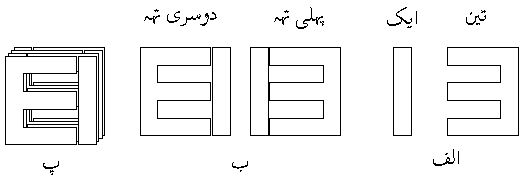
\includegraphics{figTransformersCorePlacement}
\caption{مرکزی پتری کے اشکال اور ان کو تہہ در تہہ رکھنے کا طریقہ۔}
\label{شکل_ٹرانسفارم_تہہ_در_تہہ_مرکز}
\end{figure}

ہیجان انگیز برقی رو بے بار اور بار بردار ٹرانسفارمر میں یکساں ہوتا ہے ۔جیسا کہ پہلے بھی ذکر کیا گیا ہے، قوی ٹرانسفارمر اور موٹروں میں برقی دباؤ اور مقناطیسی بہاؤ سائن نما ہوتے ہیں جبکہ ہیجان انگیز برقی رو ان میں غیر سائن نما ہوتی ہے لہٰذا اگر
\begin{gather}
\begin{aligned}
\varphi&=\phi_0 \sin \omega t=\phi_0 \cos \left(\omega t -90\degree \right)\\
\hat{\varphi}&=\phi_0 \phase{90\degree}
\end{aligned}
\end{gather}
ہو تو
\begin{gather}
\begin{aligned}
e_1&=N_1 \frac{\dif \varphi}{\dif t}=\omega N_1 \phi_0 \cos \omega t\\
\hat{E_1}&=\omega N_1 \phi_0 \phase{0}
\end{aligned}
\end{gather}
ہو\حاشیہد{اس مساوات میں اور اس کے بعد پوری کتاب میں امالی برقی دباؤ کے ساتھ منفی کی علامت نہیں لگائی جائے گی} گی۔یہاں \عددیء{\phi_0} مقناطیسی بہاؤ کے حیطہ کو ظاہر کرتی ہے،اور \عددیء{\omega} زاویاتی تعدادِ ارتعاش کو یعنی \عددیء{2 \pi f} جہاں \عددیء{f} تعدادِ ارتعاش ہے جسے ہرٹز \عددیء{\si{\hertz}} میں ناپا جاتا ہے۔\عددیء{\hat{E_1}} اور \عددیء{\hat{\varphi}} کے مابین \عددیء{90^{\circ}} کا زاویہ ہے۔یہ شکل \حوالہ{شکل_ٹرانسفارمر_مرکزی_ضیاع_اور_مقناطیسی_رو} میں دکھایا گیا ہے۔\عددیء{e_1} برقی دباؤ  کی موثر قیمت \عددیء{E_{rms}}  
\begin{align}
E_{rms}=\frac{\omega N_1 \phi_0}{\sqrt{2}}=4.44 f N_1 \phi_0
\end{align}
ہے۔اس کو ہم یوں بھی لکھ سکتے ہیں
\begin{align}
\phi_0=\frac{E_{rms}}{4.44 f N_1 \phi_0}
\end{align}

یہاں ایک بار رکھ کر دوبارہ نظر ثانی کرتے ہیں۔ اگر ایک  لچھے پر \عددیء{E_{rms}} موثر برقی دباؤ لاگو کی جائے تو یہ لچھا اتنی ہیجان انگیز برقی رو \عددیء{i_{\varphi}} گزرنے دیتی ہے جس سے نمودار ہونے والا مقناطیسی بہاؤ مساوات  میں دیئے گئے مقناطیسی بہاؤ \عددیء{\phi_0} کے برابر ہو۔ یہ بات نہ صرف ٹرانسفارمر بلکہ کسی بھی مقناطیسی دور کے لئے درست اور لازم ہے۔
\begin{figure}
\centering
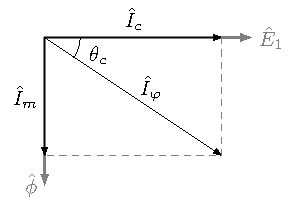
\includegraphics{figTransformersCoreLossAndMagnetizingCurrents}
\caption{مختلف دوری سمتیوں کے زاوئے۔}
\label{شکل_ٹرانسفارمر_مرکزی_ضیاع_اور_مقناطیسی_رو}
\end{figure}

غیر سائن نما ہیجان انگیز برقی رو \عددیء{\i_{\varphi}} کو فوریئر تسلسل\فرہنگ{فوریئر تسلسل}\حاشیہب{Fourier series}\فرہنگ{Fourier series} سے یوں لکھ سکتے ہیں۔
\begin{align} 
i_{\varphi}=\sum_n {\left( a_n \cos n \omega t + b_n \sin \omega t \right)}
\end{align}
اس میں \عددیء{(a_1 \cos \omega t+b_1 \sin \omega t)} کو بنیادی جزو\فرہنگ{بنیادی جزو}\حاشیہب{fundamental component}\فرہنگ{fundamental component} کہتے ہیں اور باقی حصہ کو  موسیقائی جُزو\فرہنگ{موسیقائی جزو}\حاشیہب{harmonic components}\فرہنگ{harmonic components}  کہتے ہیں۔ بنیادی جُز میں \عددیء{a_1 \cos \omega t}، مقناطیسی بہاؤ سے وجود میں آنے والے امالی برقی دباؤ \عددیء{e_1} ،  جو کہ مساوات  میں دی گئی ہے کے ہم قدم ہے۔ یعنی  یہ دونوں وقت کے ساتھ یکساں بڑھتے اور گھٹتے ہیں جبکہ اس میں \عددیء{b_1 \sin \omega t} نوّے درجہ زاویہ \عددیء{e_1}  کے پیچھے رہتا ہے۔ ان میں  \عددیء{a_1 \cos \omega t} مرکز میں مختلف وجوہات سے برقی طاقت ضائع ہونے کو ظاہر  کرتی ہے۔اسی لئے اس جُزو کو مرکزی ضیاع کا جُزو\فرہنگ{مرکزی ضیاع!جزو}\حاشیہب{core loss component}\فرہنگ{core loss component}  کہتے ہیں۔ہیجان انگیز برقی رو \عددیء{i_{\varphi}} سے اگر \عددیء{a_1 \cos \omega t} منفی کی جائے تو بقایا کو مقناطیس بنانے والا برقی رو\فرہنگ{مقناطیسی برقی رو} یا مقناطیسی برقی رو\حاشیہب{magnetizing current}\فرہنگ{magnetizing current} کہتے ہیں۔ اس  کی تیسری موسیقائی جُز سب سے زیادہ اہم  ہے۔ قوی  ٹرانسفارمروں میں یہ تیسری موسیقائی جُز عموماً  کُل ہیجان انگیز برقی رو  کے \عددیء{40} فیصد ہوتی ہے۔  

سوائے وہاں، جہاں  ہیجان انگیز برقی رو کے اثرات پر غور کیا جارہا ہو، ہم ہیجان انگیز برقی رو کے غیر سائن نما ہونے کو نظرانداز کرتے ہیں۔ قوی ٹرانسفارمر کی  ہیجان انگیز برقی رو اس کی کُل برقی رو\حاشیہد{کُل برقی رو سے مراد وہ برقی رو ہے جو کُل برقی بار لادنے سے حاصل ہو} کے صرف \عددیء{5}  فیصد کے قریب ہوتی ہے۔ لہٰذا  اس کا اثر بہت کم ہوتا ہے۔ لہٰذا ہم  ہیجان انگیز برقی رو کو سائن نما تصور کر کے اس کے اثرات پر غور کرتے ہیں۔ایسا کرنے سے مسئلہ پر غور کرنا آسان ہو جاتا ہے۔ اس فرضی سائن نما  ہیجان انگیز برقی رو\حاشیہد{یعنی  بدلتی برقی رو \عددیء{i_{\varphi}} کو اب دوری سمتیہ کی مدد سے \عددیء{\hat{I_{\varphi}}} لکھتے ہیں} \عددیء{\hat{I_{\varphi}}}  کی موثر قیمت \عددیء{I_{\varphi,rms}} ، اصل  ہیجان انگیز برقی رو کی موثر قیمت کے برابر رکھی جاتی ہے جبکہ اس کا زاویہ \عددیء{\theta_c} یوں رکھا جاتا ہے کہ اس سے حاصل برقی ضیاع اصل برقی ضیاع کے برابر ہو۔ شکل  کی مدد سے یہ بات سمجھنی زیادہ آسان ہے۔ شکل میں اگر دیکھا جائے تو
\begin{align}
p_c=E_{rms} I_{\varphi,rms} \cos \theta_c
\end{align}
جہاں \عددیء{p_c} مرکزی ضیاع  ہے۔ لہٰذا  اگر \عددیء{\hat{I_{\varphi}}} اور \عددیء{\hat{E_1}} کے مابین \عددیء{\theta_c} کا زاویہ ہو تو اس سے مرکزی ضیاع صحیح حاصل ہوتا ہے۔\عددیء{\hat{I_{\varphi}}} اسی زاویہ  سے  \عددیء{\hat{E_1}}  کے پیچھے رہتا ہے۔

\حصہ{تبادلہ برقی دباؤ اور تبادلہ برقی رو کے خصوصیات}
ہم شکل \حوالہ{شکل_ٹرانسفارمر_کامل_بار_بردار_ٹرانسفارمر}  کی مدد سے ٹرانسفارمر کا مطالعہ کرتے ہیں۔  ہم فرض کرتے ہیں کہ ابتدائی جانب لچھے کے \عددیء{N_1} اور ثانوی جانب لچھے کے \عددیء{N_2} چکر ہیں اور یہ کہ ان  دونوں لچھوں کی مزاحمت صفر ہے۔ ہم مزید یہ کہتے ہیں کہ پوری مقناطیسی بہاؤ  مرکز ہی میں رہتا ہے اور دونوں لچھوں سے گزرتا ہے۔ مرکز میں برقی توانائی ضائع نہیں ہوتی اور اس کی مقناطیسی مستقل اتنی زیادہ ہے کہ ہیجان انگیز برقی رو قابلِ نظر انداز ہے۔ برقی رو \عددیء{i_1}  اور \عددیء{i_2} کی سمتیں یوں رکھی گئی ہیں کہ ان سے وجود میں آنے والے مقناطیسی بہاؤ ایک دوسرے کی اُلٹ سمتوں میں  ہیں۔ اصل ٹرانسفارمر ان باتوں پر تقریباً پورے اترتے ہیں۔ ایسے ٹرانسفارمر کو کامل ٹرانسفارمرفرہنگ{ٹرانسفارمر!کامل}\حاشیہب{ideal transformer}\فرہنگ{transformer!ideal}  کہتے ہیں۔
\begin{figure}
\centering
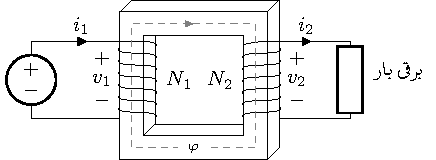
\includegraphics{figTransformersLoadedIdealTransformer}
\caption{ایک کامل بار بردار ٹرانسفارمر۔}
\label{شکل_ٹرانسفارمر_کامل_بار_بردار_ٹرانسفارمر}
\end{figure}

جب اس کامل ٹرانسفارمر کے ابتدائی لچھے پر بدلتی برقی دباؤ \عددیء{v_1} لاگو کیا جائے تو اس کے مرکز میں بدلتا مقناطیسی بہاؤ  \عددیء{\varphi_m} وجود میں  آئے گا جو ابتدائی لچھے میں   لاگو برقی دباؤ \عددیء{v_1} کے برابر امالی برقی دباؤ \عددیء{e_1} کو جنم دے گا۔لہٰذا
\begin{align}
v_1=e_1=N_1 \frac{\dif \varphi_m}{\dif t}
\end{align}
یہ مقناطیسی بہاؤ دوسرے لچھے سے بھی گزرے گا اور اس میں \عددیء{e_2} امالی برقی دباؤ کو جنم دے گا جو ثانوی جانب کے سروں پر برقی دباؤ \عددیء{v_2}  کی صورت میں حاصل ہوگا۔ یعنی
\begin{align}
v_2=e_2=N_2 \frac{\dif \varphi_m}{\dif t}
\end{align}
ان دونوں کی نسبت سے
\begin{align}\label{مساوات_ٹرانسفارمر_تبادلہ_دباؤ}
\frac{v_1}{v_2}=\frac{N_1 \frac{\dif \varphi_m}{\dif t}}{N_2 \frac{\dif \varphi_m}{\dif t}}=\frac{N_1}{N_2}
\end{align}
لہٰذا ایک کامل ٹرانسفارمر دونوں لچھوں کے چکروں کی نسبت سے برقی دباؤ کا تبادلہ\فرہنگ{برقی دباؤ!تبادلہ}\حاشیہب{voltage transformation}\فرہنگ{voltage!transformation} کرتا ہے۔

چونکہ یہ ایک کامل ٹرانسفارمر ہے لہٰذا اسے جتنی برقی طاقت ابتدائی جانب  دی جائے اتنی ہی برقی طاقت اس سے ثانوی جانب حاصل ہو گی،یعنی
\begin{align}
p=v_1 i_1 = v_2 i_2
\end{align}
یا
\begin{align}
\frac{v_1}{v_2}=\frac{i_2}{i_1}
\end{align}
مساوات  \حوالہ{مساوات_ٹرانسفارمر_تبادلہ_دباؤ} کی مدد سے
\begin{align}
\frac{v_1}{v_2}=\frac{i_2}{i_1}=\frac{N_1}{N_2}
\end{align}
یہ ایک انتہائی اہم نتیجہ ہے جو ٹرانسفارمر کی تبادلہ برقی دباؤ اور تبادلہ برقی رو\فرہنگ{برقی رو!تبادلہ}\حاشیہب{current transformation}\فرہنگ{current!transformation}  کی خصوصیات بیان کرتا ہے۔اسے عموما ً دو حصوں میں یوں لکھا جاتا ہے۔
\begin{gather}
\begin{aligned}\label{مساوات_ٹرانسفارمر_تبادلہ_دباو_رو}
\frac{v_1}{v_2}&=\frac{N_1}{N_2}\\
\frac{i_1}{i_2}&=\frac{N_2}{N_1}
\end{aligned}
\end{gather}
اس مساوات کی پہلی جُز کہتی ہے کہ ٹرانسفارمر کی دونوں جانب برقی دباؤ  ان کے چکروں کی راست متناسب  ہو گا جبکہ مساوات کی دوسری جُز کہتی ہے کہ ٹرانسفارمر کے دونوں جانب برقی رو ان کے چکروں کے بالعکس متناسب ہو گا۔

\ابتدا{مثال}
	شکل میں اگر
\begin{align*}
\hat{V_1}&=220 \phase{0}\\
N_1:N_2&=220:22\\
Z&=R=\SI{10}{\ohm}
\end{align*}
ہوں تو ٹرانسفارمر کی دونوں جانب برقی دباؤ اور برقی رو معلوم کریں۔

حل:
ابتدائی جانب برقی دباؤ دیا گیا ہے یعنی \عددیء{220} وولٹ جبکہ ثانوی جانب برقی دباؤ مساوات \حوالہ{مساوات_ٹرانسفارمر_تبادلہ_دباو_رو} کی پہلی جُز کی مدد سے حاصل کیا جاتا ہے یعنی
\begin{align*}
\hat{V_2}=\frac{N_2}{N_1} \hat{V_1}=\frac{22}{220} \times 220\phase {0}=22\phase{0}
\end{align*}
ثانوی جانب \عددیء{22} وولٹ ہیں جو ابتدائی جانب برقی دباؤ کے ہم قدم ہے۔ثانوی جانب یہ برقی دباؤ \عددیء{10} اوہم کی مزاحمت میں برقی رو پیدا کرے گا جسے اوہم کے قانون سے حاصل کیا جاتا ہے یعنی
\begin{align*}
\hat{V_2}=\frac{22 \phase {0}}{10}=2.2\phase {0}
\end{align*}
ثانوی جانب \عددیء{2.2} ایمپیئر برقی رو ہے۔ ابتدائی جانب کی برقی رو مساوات \حوالہ{مساوات_ٹرانسفارمر_تبادلہ_دباو_رو} کی دوسری جُز کی مدد سے حاصل کی جاتی ہے یعنی
\begin{align*}
\hat{I_1}=\frac{N_2}{N_1} \hat{I_2}=\frac{22}{220} \times 2.2\phase{0}=0.22\phase{0}
\end{align*}
\انتہا{مثال}

اس مثال کے نتائج ایک جگہ لکھ کر ان پر غور کرتے ہیں۔
\begin{align*}
\hat{V_1}=220\phase{0}, \quad \hat{V_2}=22\phase{0}, \quad \hat{I_1}=0.22\phase{0}, \quad \hat{I_2}=2.2\phase{0}
\end{align*}
ہم دیکھتے ہیں ابتدائی جانب برقی دباؤ ثانوی جانب کی برقی دباؤ کے دس گنا ہے جبکہ برقی رو میں قصہ اُلٹ ہے۔ثانوی جانب کی برقی رو ابتدائی جانب کی برقی رو کے دس گنا ہے۔طاقت دونوں جانب برابر ہے۔یہ نہایت اہم ہے کہ آپ اس بات کو اچھی طرح سمجھ لیں کہ جس جانب برقی دباؤ زیادہ ہوتا ہے اس جانب برقی رو کم ہوتی ہے۔ لہٰذا زیادہ برقی دباؤ کی جانب لچھے کے چکر زیادہ ہوں گے اور اس لچھے میں نسبتاً باریک برقی تار استعمال ہوگی جبکہ کم برقی دباؤ کا لچھا کم چکر کا ہو گا اور اس میں نسبتاً موٹی برقی تار استعمال ہو گی۔ 

\ابتدا{مثال}
	شکل الف سے رجوع کریں۔ اس شکل میں مقاومت \عددیء{Z_2} کو  بدلتی برقی دباؤ \عددیء{\hat{V_1}} کے ساتھ ایک ٹرانسفارمر کے ذریعہ جوڑا گیا ہے۔اگر
\begin{align*}
\hat{V_1}=110\phase{0},\quad Z_2=R+j X=3+j 2,\quad N_1:N_2=220:22 
\end{align*}
ہوں تو مقاومت میں برقی رو اور طاقت کا ضیاع معلوم کریں۔

حل:
	ٹرانسفارمر کی تبادلہ برقی دباؤ کی خصوصیت سے اس کے ابتدائی جانب \عددیء{110} وولٹ برقی دباؤ ٹرانسفارمر کی ثانوی جانب تبدیل ہوکر  \عددیء{\hat{V_s}} ہو جائیں گے جہاں
\begin{align*}
\hat{V_s}=\frac{N_2}{N_1} \hat{V_1}=\frac{22}{220} \times 110\phase{0}=11\phase{0}
\end{align*}
ہے لہٰذا
\begin{align*}
\hat{I_2}=\frac{\hat{V_s}}{Z}=\frac{11\phase{0}}{3+j 2}= -3.05\phase{-33.69\degree}
\end{align*}
اور برقی طاقت کا ضیاع \عددیء{p_z}
\begin{align*}
p_z=I_2^2 R=3.05^2 \times 3=\SI{27.9}{\watt}
\end{align*}
\انتہا{مثال}

\حصہ{ثانوی جانب بار کا ابتدائی جانب اثر}
یہاں شکل  سے رجوع کریں۔ہم حصہ  میں دیکھ چکے ہیں کہ اگر ایک بے بار ٹرانسفارمر کی ابتدائی لچھے پر بدلتی برقی دباؤ \عددیء{v_1} لاگو کی جائے تو اس لچھے میں ہیجان انگیز برقی رو \عددیء{i_{\varphi}} گزرے گی۔اس برقی رو کی مقناطیسی دباؤ \عددیء{N_1 i_{\varphi}} مرکز میں مقناطیسی بہاؤ \عددیء{\varphi_m}\حاشیہد{\عددیء{\varphi} کو یہاں \عددیء{\varphi_m} کہا گیا ہے۔} کو جنم دے گی ۔اگر لچھے کی مزاحمت صفر ہو تو \عددیء{\varphi_m} ابتدائی لچھے میں \عددیء{e_1} امالی برقی دباؤ پیدا کرے گی جہاں
\begin{align*}
v_1=e_1=N_1 \frac{\dif \varphi_m}{\dif t}
\end{align*}
ہو گی۔

اب ہم ثانوی جانب  برقی بار لادتے ہیں۔ ایسا کرنے سے بار بردار ٹرانسفارمر\فرہنگ{ٹرانسفارمر!بار بردار}\حاشیہب{loaded transformer}  کے  ثانوی جانب  برقی رو \عددیء{i_2} رواں ہوگی جس کی وجہ سے \عددیء{N_2 i_2} مقناطیسی دباؤ وجود میں آئیگی۔ اس مقناطیسی دباؤ کی وجہ سے مرکز میں مقناطیسی بہاؤ \عددیء{\varphi_{\textup{بار}}}  پیدا ہوگا۔ اگر اس مقناطیسی بہاؤ کا کچھ  نہ کیا جائے تو مرکز میں پہلے سے موجود مقناطیسی بہاؤ تبدیل ہو کر \عددیء{\varphi_{\textup{نئی}}=\varphi_{m}-\varphi_{\textup{بار}}} ہو جائے گا اور یوں ابتدائی لچھے میں امالی دباؤ تبدیل ہو کر \عددیء{e_{\textup{نئی}}} ہو جائے گا۔  لہٰذا ابتدائی جانب پر اب امالی دباؤ اور اس پر لاگو برقی دباؤ برابر نہیں ہونگے جو کہ مساوات  کی موجودگی میں ناممکن ہے۔ لہٰذا اس مقناطیسی بہاؤ \عددیء{\varphi_{\textup{بار}}}  کے اثر کو ختم کرنے کیلئے ابتدائی لچھے میں برقی رو \عددیء{i_{1}} نمودار ہو گی جو اس مقناطیسی دباؤ یعنی \عددیء{N_2 i_2} کے اثر کو ختم کر دے گی یعنی
\begin{align}
N_1 i_1=N_2 i_2
\end{align}
یہ وہ ذریعہ ہے جس سے ابتدائی جانب معلوم ہوتا ہے کہ ثانوی جانب پر بار لدا ہے۔ شکل میں دونوں لچھوں میں برقی رو کی سمتیں یوں ہیں کہ ان کے مقناطیسی بہاؤ آپس میں اُلٹ سمت میں ہیں لہٰذا  مرکز میں اب پھر مقناطیسی بہاؤ \عددیء{\varphi_m}  کے برابر  ہے جیسا کہ ہونا چاہئے تھا۔ اس مساوات کو یوں لکھ سکتے ہیں
\begin{align}
\frac{i_1}{i_2}=\frac{N_2}{N_1}
\end{align}
یہ وہی مساوات ہے جو کامل ٹرانسفارمر کے لئے ثابت کی گئی تھی۔
%
\حصہ{ٹرانسفارمر کی علامت پر نقطوں کا مطلب}
	شکل  میں ٹرانسفارمر کے لچھوں پر نکتے لگائے گئے ہیں۔ یہ نکتے اس بات کو ظاہر کرتے ہیں کہ اگر ایک طرف کے لچھے پر برقی دباؤ \عددیء{v_1} یوں ہو کہ نکتے والا سرا مثبت اور بغیر نکتے والا سرا منفی ہو تو دوسرے لچھے  پر برقی دباؤ \عددیء{v_2} اس طرح ہو گا کہ اس لچھے کا بھی  نکتے والا سرا مثبت اور بغیر نکتے والا سرا منفی ہوگا۔

مزید یہ کہ ابتدائی جانب برقی رو ٹرانسفارمر کے نکتے والے سرے سے ٹرانسفارمر کی اندر جانب ہو گا جبکہ ثانوی جانب برقی رو نقطہ والے سرے سے ٹرانسفارمر سے باہر نکلے گا۔

 یوں  \عددیء{v_1} اور \عددیء{v_2} وقت کے ساتھ یکساں تبدیل ہوتے ہیں اور ان کے مابین صفر زاویہ ہے۔ لہٰذا یہ دو برقی دباؤ ہم قدم\فرہنگ{ہم قدم}\حاشیہب{in-phase}\فرہنگ{in-phase} ہیں۔

\حصہ{مقاومت کا تبادلہ}
اس حصہ میں کامل ٹرانسفارمر میں مقاومت کے تبادلہ پر غور کیا جائے گا۔شکل \حوالہ{شکل_ٹرانسفارمر_مقاومت_کا_تبادلہ}-الف میں ایک ٹرانسفارمر دکھایا گیا ہے جس کی ابتدائی جانب سائن نما برقی دباؤ  \عددیء{\hat{V_1}=V_1\phase{\theta}}  لاگو کیا گیا ہے۔یہاں دوری سمتیہ استعمال کئے جائیں گے۔

جیسے اُوپر ذِکر ہوا، برقی دباؤ \عددیء{\hat{V_1}} اور \عددیء{\hat{V_2}} آپس میں ہم قدم ہیں اور  اسی طرح برقی رو \عددیء{\hat{I_1}} اور \عددیء{\hat{I_2}} آپس میں  ہم قدم ہیں۔ مساوات   کو دوری سمتیہ کی مدد سے یوں لکھ سکتے ہیں
\begin{gather}
\begin{aligned}
\hat{V_1}&=\left(\frac{N_1}{N_2} \right) \hat{V_2}\\
\hat{I_1}&=\left(\frac{N_2}{N_1} \right) \hat{I_2}
\end{aligned}
\end{gather}
چونکہ مقاومت
\begin{align}
Z_2=\frac{\hat{V_2}}{\hat{I_2}}=\abs{Z_2}\phase{\theta_z}
\end{align}
کے برابر ہے لہٰذا
\begin{align}\label{مساوات_ٹرانسفارمر_تبادلہ_مقاومت_الف}
\frac{\hat{V_1}}{\hat{I_1}}=\left(\frac{N_1}{N_2} \right)^2 \frac{\hat{V_2}}{\hat{I_2}}=\left(\frac{N_1}{N_2} \right)^2  Z_2
\end{align}
اب اگر ہم ٹرانسفارمر بمع اس پر لدھے مقاومت  کی جگہ برقی دباؤ \عددیء{\hat{V_1}} کو مقاومت \عددیء{Z_1} پر لاگو کریں جہاں اس مقاومت کی قیمت
\begin{align}\label{مساوات_ٹرانسفارمر_متبادل_مقاومت_تعریف}
Z_1=\left(\frac{N_1}{N_2} \right)^2  Z_2
\end{align}
ہو تو \عددیء{\hat{V_1}} سے حاصل برقی رو یا اس سے حاصل برقی طاقت تبدیل نہیں ہو گی۔یہ شکل ب میں دکھایا گیا ہے جہاں سے واضح ہے کہ
\begin{align}\label{مساوات_ٹرانسفارمر_تبادلہ_مقاومت_ب}
\frac{\hat{V_1}}{\hat{I_1}}=Z_1=\left(\frac{N_1}{N_2} \right)^2  Z_2
\end{align}
لہٰذا شکل کے الف اور با دونوں حصوں سے  برقی دباؤ \عددیء{\hat{V_1}} کی برقی رو مساوات \حوالہ{مساوات_ٹرانسفارمر_تبادلہ_مقاومت_الف}  اور \حوالہ{مساوات_ٹرانسفارمر_تبادلہ_مقاومت_ب}  سے یکساں حاصل ہوتی ہے یعنی
\begin{align}
\hat{I_1}=\frac{\hat{V_1}}{\left(\frac{N_1}{N_2} \right)^2  Z_2}
\end{align}
اور یوں الف اور با  دونوں حصوں میں  برقی دباؤ \عددیء{\hat{V_1}} سے حاصل برقی طاقت برابر ہے یعنی
\begin{align}
p=\hat{V_1} \cdot \hat{I_1}=\frac{V_1^2 \cos \theta_z}{\left(\frac{N_1}{N_2} \right)^2  \abs{Z_2}}
\end{align}
%
\begin{figure}
\centering
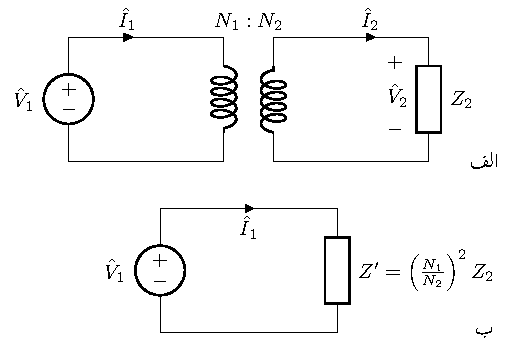
\includegraphics{figTransformersImpedanceTransformation}
\caption{ٹرانسفارمر کی تبادلہ مقاومت کی خصوصیت۔}
\label{شکل_ٹرانسفارمر_مقاومت_کا_تبادلہ}
\end{figure}
	یوں اگر ٹرانسفارمر کے ثانوی جانب  مقاومت \عددیء{Z_2} کا بار ہو تو حساب کرتے وقت ہم یہ اخذ کر سکتے ہیں کہ  ٹرانسفارمر بمع مقاومت \عددیء{Z_2} کی  جگہ  صرف  \عددیء{Z_1} مقاومت لگی ہے، جہاں \عددیء{Z_1} مساوات \حوالہ{مساوات_ٹرانسفارمر_متبادل_مقاومت_تعریف}  سے حاصل ہوتی ہے۔ مقاومت کا یوں ٹرانسفارمر کی ایک جانب سے دوسری جانب تبادلہ کیا جاسکتا ہے۔ٹرانسفارمر کی اس خاصیت کو  تبادلہ مقاومت\فرہنگ{تبادلہ!مقاومت}\حاشیہب{impedance transformation}\فرہنگ{impedance transformation} کی خصوصیت  کہتے ہیں۔
%
\ابتدا{مثال}
شکل \حوالہ{شکل_ٹرانسفارمر_برقی_طاقت_کی_منتقلی}-الف میں مقاومت \عددیء{Z_B} کا برقی بار ایک جنریٹر پر لدھا ہے۔بار تک برقی طاقت دو برقی تاروں کے ذریعہ منتقل کیا گیا ہے۔ان تاروں کی مجموعہ مقاومت \عددیء{Z_t} ہے۔
\begin{figure}
\centering
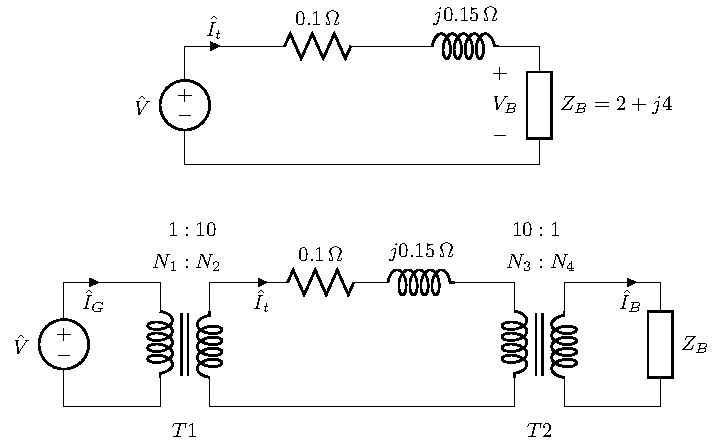
\includegraphics{figTransformersPowerTransmission}
\caption{برقی طاقت کی منتقلی۔}
\label{شکل_ٹرانسفارمر_برقی_طاقت_کی_منتقلی}
\end{figure}
%
\begin{figure}
\centering
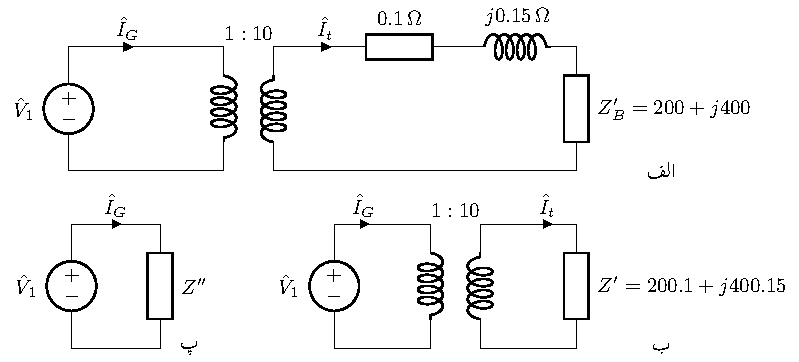
\includegraphics{figTransformersStepByStepSolution}
\caption{ٹرانسفارمر قدم با قدم حل کرنے کا طریقہ۔}
\label{شکل_ٹرانسفارمر_قدم_با_قدم_حل}
\end{figure}

شکل-ب میں جنریٹر کے قریب نسب برقی دباؤ بڑھانے والا ٹرانسفارمر برقی دباؤ کو دس گنا بڑھاتا ہے اور برقی بار کے قریب نسب برقی دباؤ گھٹانے والا ٹرانسفارمر برقی دباؤ کو دس گنا گھٹاتا ہے۔اس حصہ میں وہی برقی تار استعمال کئے گئے ہیں لہٰذا ان کی بھی مجموعہ مقاومت \عددیء{Z_t} ہی ہے۔
اگر 
\begin{align*}
Z_B=2+j 4, \quad Z_t=0.1 +j 0.15, \quad \hat{V}=415\phase{0}
\end{align*}
ہوں تو دونوں صورتوں میں
\begin{itemize}
\item
برقی بار پر برقی دباؤ معلوم کریں،
\item
برقی تاروں میں برقی طاقت کی ضیاع معلوم کرین۔
\end{itemize}

حل الف:
\begin{align*}
\hat{I_G}=\hat{I_t}=\hat{I_B}&=\frac{\hat{V}}{Z_t+Z_B}=\frac{415\phase{0}}{0.1+j 0.15+2+j 4}\\
&=\frac{415\phase{0}}{2.1+j 4.15}=89.23\phase{-63.159\degree}\\
&=40.3-j79.6
\end{align*}
یوں مقاومت پر برقی دباؤ
\begin{align*}
\hat{V_B}=\hat{I_B} Z_B&=\left(40.3-j79.6 \right) \left( 2+j 4\right)\\
&=399+j2=399\phase{0.287\degree}
\end{align*}
اور برقی تاروں میں برقی طاقت کا ضیاع ہے
\begin{align*}
p_t=I_t^2 R_t=89.23^2 \times 0.1=\SI{796}{\watt}
\end{align*}

حل ب:
شکل \حوالہ{شکل_ٹرانسفارمر_برقی_طاقت_کی_منتقلی} اور شکل \حوالہ{شکل_ٹرانسفارمر_قدم_با_قدم_حل}  سے رجوع کریں۔شکل  \حوالہ{شکل_ٹرانسفارمر_برقی_طاقت_کی_منتقلی} میں ٹرانسفارمر \عددیء{T_2} کے ثانوی جانب مقاومت کا مساوات  کی مدد سے اس کی ابتدائی جانب تبادلہ سے ملتا ہے
\begin{align*}
Z_B'=Z_1=\left(\frac{N_3}{N_4} \right)^2 Z_B=\left(\frac{10}{1} \right)^2 \left(2+j 4 \right)=200+j 400
\end{align*}
یوں شکل \حوالہ{شکل_ٹرانسفارمر_قدم_با_قدم_حل}-الف حاصل ہوتا ہے۔اس شکل میں اب برقی تار کی مقاومت اور  تبادلہ شدہ مقاومت سلسلہ وار جُڑے ہیں۔ان کے مجموعہ  کو \عددیء{Z'} کہتے ہوئے
\begin{align*}
Z'=Z_t+Z_B'=0.1+j 0.15+200+j 400=200.1+j400.15
\end{align*}
یہ شکل \حوالہ{شکل_ٹرانسفارمر_قدم_با_قدم_حل}-ب میں دکھایا گیا ہے۔ایک مرتبہ دوبارہ مساوات  استعمال کرتے ہوئے
\begin{align*}
Z''=\left(\frac{N_1}{N_2} \right)^2 Z'=\left(\frac{1}{10} \right)^2 \left(200.1+j400.15 \right)=2.001+j4.0015
\end{align*}
شکل \حوالہ{شکل_ٹرانسفارمر_قدم_با_قدم_حل}-پ میں دکھایا گیا ہے۔اب
\begin{align*}
\hat{I_G}=\frac{\hat{V}}{Z''}=\frac{415\phase{0}}{2.001+j4.0015}=92.76\phase{-63.432\degree}
\end{align*}
یہاں سے شکل \حوالہ{شکل_ٹرانسفارمر_قدم_با_قدم_حل}-ب  کی مدد سے اگر جنریٹر کی برقی رو معلوم ہو تو تبادلہ برقی رو سے
\begin{align*}
\hat{I_t}=\left(\frac{N_1}{N_2} \right) \hat{I_G}=\left(\frac{1}{10}\right) 92.76\phase{-63.432\degree}=9.276\phase{-63.432\degree}
\end{align*}
اس سے برقی تار میں طاقت کا ضیاع
\begin{align*}
p_t=I_t^2 R_t=9.276^2  \times 0.1=\SI{8.6}{\watt}
\end{align*}
اسی طرح شکل \حوالہ{شکل_ٹرانسفارمر_برقی_طاقت_کی_منتقلی}  میں اگر \عددیء{\hat{I_t}} معلوم ہو تو تبادلہ برقی رو سے
\begin{align*}
\hat{I_B}&=\left(\frac{N_3}{N_4}\right) \hat{I_t}=\left(\frac{10}{1}\right) 9.276\phase{-63.432\degree}\\
&=92.76\phase{-63.432\degree}=41.5-j 82.9
\end{align*}
اور مقاومت پر برقی دباؤ
\begin{align*}
\hat{V_B}=\hat{I_B} Z_B=\left(41.5-j 82.9 \right) \left(2+j 4 \right)=414+j 0.2
\end{align*}
ہو گی۔

ٹرانسفارمر کے بغیر برقی طاقت کی منتقلی میں برقی تاروں میں طاقت کی ضیاع \عددیء{796} واٹ ہے جبکہ ٹرانسفارمر کے استعمال سے یہ صرف \عددیء{8.6} واٹ ہے یعنی \عددیء{92} گنا کم۔یہی ٹرانسفارمر کی نہایت مقبولیت کی وجہ ہے۔ 
\انتہا{مثال}
%
\حصہ{ٹرانسفارمر کے وولٹ-ایمپیئر}
ٹرانسفارمر کی دونوں جانب برقی دباؤ ان لچھوں کے چکر پر منحصر ہوتا ہے۔ٹرانسفارمر ایک خاص برقی دباؤ اور برقی رو کے لئے بنائے جاتے ہیں۔ٹرانسفارمر جس برقی دباؤ \عددیء{V_1:V_2} کے لئے بنائے جائیں یہ اس سے کم برقی دباؤ پر بھی استعمال کئے جا سکتے ہیں اگرچہ یہ عموما ً بنائے گئے برقی دباؤ پر ہی چلائے جاتے ہیں۔اسی طرح ٹرانسفارمر جتنی برقی رو \عددیء{I_1:I_2} کے لئے بنائے جائیں انہیں اس سے کم برقی رو پر استعمال کیا جا سکتا ہے۔حقیقت میں عموما ً ٹرانسفارمر سے حاصل برقی رو اس حد سے کم ہی رکھی جاتی ہے۔

ٹرانسفارمر کی ایک جانب کی برقی دباؤ اور برقی رو کا حاصل ضرب اس کی دوسری جانب کی برقی دباؤ اور برقی رو کے حاصل ضرب کے برابر ہوتا ہے یعنی
\begin{align}
V_1 I_1=V_2 I_2
\end{align}
برقی دباؤ اور برقی رو کے حاصلِ ضرب  یعنی \عددیء{V_1 I_1} یا \عددیء{V_2 I_2} کو ٹرانسفارمر کی وولٹ ضربِ ایمپیئر کہتے ہیں جسے عموما ً چھوٹا کر کے صرف وولٹ-ایمپیئر\فرہنگ{وولٹ-ایمپیئر}
\حاشیہب{volt-ampere, VA}\فرہنگ{volt-ampere}\فرہنگ{VA}  کہا جاتا ہے\حاشیہد{وولٹ-ایمپیئر کو عموما ً کلو وولٹ-ایمپیئر یعنی \عددیء{\si{\kilo \volt \ampere}} میں بیان کیا جاتا ہے}۔یہ ٹرانسفارمر کی برقی اہلیت کی ناپ ہے جو اس پر لگی تختی پر لکھا جاتا ہے۔اس تختی پر ٹرانسفارمر کے برقی دباؤ اور برقی تعدادِ ارتعاش بھی لکھے جاتے ہیں۔یوں ٹرانسفارمر کے وولٹ-ایمپیئر
\begin{align}
\textup{وولٹ ایمپیئر}= V_1 I_1 = V_2 I_2
\end{align}
ہوں گے۔

اگرچہ یہاں ذکر ٹرانسفارمر کا ہو رہا ہے دراصل برقی مشین یعنی موٹر اور جنریٹر کی تختیوں پر بھی ان کے چالو حالت کے برقی دباؤ، ان کے وولٹ-ایمپیئر اور برقی تعدادِ ارتعاش لکھے جاتے ہیں۔اس کی وجہ یہ ہے کہ ان سب مشین کی کارکردگی کے بنیادی اصول ایک ہی طرح کے ہیں۔

\ابتدا{مثال}
ایک \عددیء{25000 } وولٹ-ایمپیئر اور \عددیء{11000:220} وولٹ برقی اہلیت  کے ٹرانسفارمر کے زیادہ برقی دباؤ کی جانب \عددیء{11000} وولٹ لاگو ہیں۔
\begin{itemize}
\item
اس کی ثانوی جانب زیادہ سے زیادہ کتنی برقی بار ڈالی جا سکتی ہے۔
\item
اس زیادہ سے زیادہ برقی بار پر اس کے ابتدائی لچھے میں برقی رو حاصل کریں۔
\end{itemize}

حل:	اس ٹرانسفارمر کی معلومات یہ ہیں
\begin{align*}
\SI{25}{\kilo \volt \ampere}, \quad 11000:220\,\textup{V}
\end{align*}
اس کی ثانوی جانب برقی دباؤ تبادلہ برقی دباؤ کی مساوات سے  \عددیء{220 } وولٹ حاصل ہوتا ہے۔یوں اس کی ثانوی جانب یعنی کم برقی دباؤ کی جانب زیادہ سے زیادہ برقی رو مساوات  سے حاصل کیا جاتا ہے۔
\begin{align*}
I_2=\frac{25000}{220}=\SI{113.636}{\ampere}
\end{align*}
اسی طرح اس کی ابتدائی جانب زیادہ سے زیادہ برقی رو اسی مساوات سے یوں حاصل ہوتی ہے
\begin{align*}
I_1=\frac{25000}{11000}=\SI{2.27}{\ampere}
\end{align*}
\انتہا{مثال}
%
ٹرانسفارمر کی دونوں جانب لچھوں میں استعمال برقی تار کی موٹائی یوں رکھی جاتی ہے کہ ان میں کثافتِ برقی رو \عددیء{J}\حاشیہد{\عددیء{\SI{1000}{\kilo \volt \ampere}}  ٹرانسفارمر کی لچھوں میں کثافتِ برقی رو تقریباً  \عددیء{\SI{3}{\ampere / \milli \meter \squared}} رکھی جاتی ہے} یکساں ہو۔لچھوں کی مزاحمت میں برقی رو گزرنے سے برقی طاقت کا ضیاع ہوتا ہے جس سے یہ گرم ہوتے ہیں۔ٹرانسفارمر کی برقی رو کی حد لچھوں کی گرمائش پر منحصر ہوتی ہے۔ان کی زیادہ سے زیادہ حرارت کو محفوظ حد کے اندر رکھا جاتا ہے۔

بڑے ٹرانسفارمر کے مرکز اور لچھے ایک غیر موصل تیل سے بھری ٹینکی میں ڈبوئے رکھے جاتے ہیں۔یہ تیل ایک تو برقی لچھوں کی حرارت کم کرنے میں مدد دیتا ہے اور دوسری جانب غیر موصل ہونے کی وجہ سے یہ زیادہ برقی دباؤ کے حصوں کو برقی طور پر جدا رکھنے میں مدد دیتا ہے۔یہ تیل تقریباً  \عددیء{\SI{80}{\celsius}} پر خراب ہونا شروع ہو جاتا ہے اور ہر \عددیء{\SI{8}{\celsius}} اضافی درجہ حرارت پر اس کی زندگی آدھی ہوتی رہتی ہے۔یعنی اگر \عددیء{\SI{80}{\celsius}} پر تیل کی کارآمد زندگی \عددیء{x} سال ہے تو \عددیء{\SI{88}{\celsius}} پر \عددیء{x/2} سال اور  \عددیء{\SI{96}{\celsius}} پر یہ صرف  \عددیء{x/4} سال ہو گی۔

	ٹرانسفارمر جس برقی دباؤ کے لئے بنایا جائے  یہ اس پر لگی تختی پر لکھا جاتا ہے۔اس سے حاصل برقی رو کی حد کو ایک مختلف طریقے سے لکھا جاتا ہے۔

\حصہ{ٹرانسفارمر کے امالہ اور اس کے مساوی دور}
\جزوحصہ{لچھے کی مزاحمت اور اس کی متعاملہ علیحدہ کرنا}
ٹرانسفارمر کی ابتدائی لچھے کی مزاحمت \عددیء{R_1} کو ہم نے حصہ مساوات میں دیکھا۔لچھے کی مزاحمت کو لچھے سے باہر لچھے کے ساتھ سلسلہ وار جڑا دکھایا گیا تھا۔دیکھتے ہیں یہ کیسے ممکن ہوتا ہے۔

شکل \حوالہ{شکل_ٹرانسفارمر_لچھے_کی_مزاحمت_اور_متعاملہ}-الف میں ایک لچھے پر بدلتی برقی دباؤ لاگو کا گیا ہے۔اگر لچھے کی برقی تار کو نہایت چھوٹے ٹکڑوں میں تقسیم کیا جائے تو اس کے ہر ٹکڑے کی نہایت کم مزاحمت  اور متعاملہ ہو گی۔ایسا ایک ٹکڑا شکل-ب میں دکھایا گیا ہے۔چونکہ لچھا ان سب ٹکڑوں کے سلسلہ وار جڑنے سے بنا ہے  لہٰذا شکل-الف کو ہم شکل-پ کی طرح بنا سکتے ہیں جہاں لچھے کے \عددیء{n} ٹکڑے  کیے گیے ہیں۔
\begin{figure}
\centering
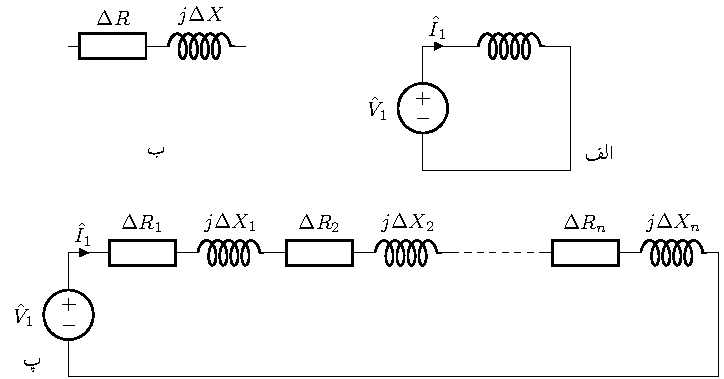
\includegraphics{figTransformersCoilResistanceAndReactance}
\caption{لچھے کی مزاحمت اور متعاملہ۔}
\label{شکل_ٹرانسفارمر_لچھے_کی_مزاحمت_اور_متعاملہ}
\end{figure}

اس دور کی مساوات لکھ کر حل کرتے ہیں۔
\begin{align*}
\hat{V}_1&=\hat{I}_1 \left(\Delta R_1 + j \Delta X_1 +\Delta R_2 + j \Delta X_2 + \cdots \Delta R_n + j \Delta X_n   \right)\\
&=\hat{I}_1 \left(\Delta R_1 +\Delta R_2 +\cdots \Delta R_n   \right)+\hat{I}_1 \left(j \Delta X_1 + j \Delta X_2+\cdots   j \Delta X_n   \right)\\
&=\hat{I}_1 \left( R +j X \right)
\end{align*}
جہاں
\begin{align*}
R&=\Delta R_1 +\Delta R_2 +\cdots \Delta R_n\\
X&=\Delta X_1 + \Delta X_2 +\cdots   \Delta X_n
\end{align*}
اس سے  شکل \حوالہ{شکل_ٹرانسفارمر_لچھے_کی_مزاحمت_اور_متعاملہ_کی_علیحدگی}  حاصل ہوتا ہے  جس سے  ثابت ہوتا ہے کہ حساب کتاب کی غرض سے لچھے کی مزاحمت اور متعاملہ علیحدہ کیئے جا سکتے ہیں۔
\begin{figure}
\centering
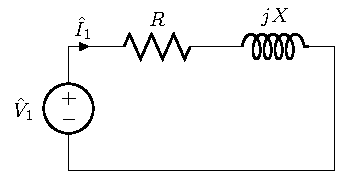
\includegraphics{figTransformersCoilResistanceAndReactanceSeparation}
\caption{لچھے کی مزاحمت اور متعاملہ کی علیحدگی۔}
\label{شکل_ٹرانسفارمر_لچھے_کی_مزاحمت_اور_متعاملہ_کی_علیحدگی}
\end{figure}
%
\جزوحصہ{رِستا امالہ}
اوپر ایک کامل ٹرانسفارمر زیرِ بحث رہا۔ اب ہم ٹرانسفارمر میں ان عناصر کا ذکر کرتے ہیں جن کی وجہ سے ٹرانسفارمر غیر کامل ہو جاتا ہے۔ بہت سی جگہوں پر ٹرانسفارمر استعمال کرتے وقت ان عناصر کو مدِ نظر رکھ کر ہی اس کا صحیح استعمال ممکن ہوتا ہے۔ ان عناصر کے اثر کو شامل کرنے کے لئے ہم  ٹرانسفارمر کا مساوی دور بناتے ہیں۔

ابتدائی لچھے کے مقناطیسی بہاؤ کو دو حصوں میں تقسیم کیا جا سکتا ہے۔ پہلا حصہ وہ جو مرکز سے گزر کر ابتدائی اور ثانوی لچھے دونوں سے گزرتا ہے۔ یہ ان کا مشترکہ مقناطیسی بہاؤ ہے اور دوسرا حصہ وہ جو صرف ابتدائی لچھے سے گزرتا ہے اور زیادہ تر مرکز کے باہر خلاء میں ہی رہتا ہے۔  اس کو رستا  مقناطیسی بہاؤ\فرہنگ{مقناطیسی بہاؤ!رستا}\حاشیہب{leakage magnetic flux}\فرہنگ{magnetic flux!leakage}   کہتے ہیں۔ یہ شکل میں دکھایا گیا ہے۔ چونکہ ہوا میں مقناطیسی مستقل \عددیء{\mu_0} مقررہ ہے لہٰذا یہاں ہچکچاہٹ بھی مقررہ ہے۔  یوں رستا مقناطیسی بہاؤ ابتدائی لچھے کی برقی رو کے  براہ راست متناسب ہوتی ہے۔

 اس کے اثر کو بالکل لچھے کی مزاحمت کی طرح لچھے سے باہر رستا امالہ\فرہنگ{رستا!امالہ}\حاشیہب{leakage inductance}\فرہنگ{leakage inductance} \عددیء{L_1} یا رستا متعاملہ\فرہنگ{رستا!متعاملہ}\حاشیہب{leakage reactance}\فرہنگ{leakage reactance}  \عددیء{X_1=2\pi f L_1} سے ظاہر کیا جاتا ہے۔

ٹرانسفارمر کے ابتدائی لچھے میں برقی رو \عددیء{\hat{I_1}}  گزرنے سے رستا متعاملہ میں \عددیء{\hat{V}_{X1}=j \hat{I}_1 X_1} برقی دباؤ اور لچھے کے تار کی مزاحمت \عددیء{R_1} میں
 \عددیء{\hat{V}_{R1}=\hat{I}_1 R_1} برقی دباؤ گھٹتا ہے۔

یوں ابتدائی لچھے  پر لاگو برقی دباؤ \عددیء{\hat{V}_1} میں سے کچھ برقی دباؤ \عددیء{R_1} میں کم ہو گا،  کچھ  متعاملہ \عددیء{X_1} میں کم ہو گا اور بقایا  \عددیء{\hat{E}_1} کے برابر ہوگا۔  یہ شکل \حوالہ{شکل_ٹرانسفارمر_ماڈل_حصہ_اول}  میں دکھایا گیا ہے۔
\begin{figure}
\centering
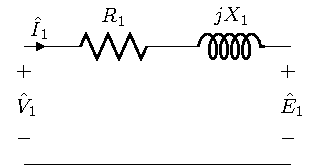
\includegraphics{figTransformersModelFirstPart}
\caption{ٹرانسفارمر مساوی دور، حصہ اول۔}
\label{شکل_ٹرانسفارمر_ماڈل_حصہ_اول}
\end{figure}
%

\جزوحصہ{ثانوی برقی رو اور مرکز کے اثرات}
مرکز میں دونوں لچھوں کا مشترکہ مقناطیسی بہاؤ ان کے مجموعی مقناطیسی دباؤ کی وجہ سے وجود میں آتا ہے۔ البتہ اگر ہم کچھ یوں سوچیں تو یہ زیادہ بہتر ہو گا۔ ہم کہتے ہیں کہ ابتدائی برقی رو کو دو شرائط پوری کرنی ہو نگی۔ پہلی یہ کہ اسے مرکز میں ہیجانی مقناطیسی بہاؤ وجود میں لانا ہوگا اور دوسری یہ کہ اسے ثانوی لچھے کے پیدا کردہ مقناطیسی بہاؤ کو ختم کرنا ہوگا۔ لہٰذا ابتدائی برقی رو کو ہم دو حصوں میں تقسیم کر سکتے ہیں۔ ایک حصہ \عددیء{i_{\varphi}} جو ہیجانی مقناطیسی بہاؤ پیدا کرے اور دوسرا \عددیء{\hat{I}_2'} جو ثانوی لچھے کے مقناطیسی دباؤ کے اثر کو ختم کرے۔ لہٰذا
\begin{align}
\hat{I}_2'=\frac{N_2}{N_1} \hat{I}_2
\end{align}
	اس باب کے حصہ  میں اس پر تفصیل سے غور کیا گیا ہے۔ برقی رو \عددیء{i_{\varphi}} غیر سائن نما ہوتی ہے لیکن پھر بھی  ہم اسے سائن نما\حاشیہد{سائن نما برقی رو کو دوری سمتیہ سے ظاہر کیا جاتا ہے} \عددیء{\hat{I}_\varphi}  ہی تصور کرتے ہیں۔ اس کو ہم دو حصوں میں تقسیم کر سکتے ہیں یعنی
\begin{align}
\hat{I}_\varphi=\hat{I}_c+\hat{I}_m
\end{align}
جہاں \عددیء{\hat{I}_c} اس کا وہ حصہ ہے جو ابتدائی لچھے کی امالی برقی دباؤ \عددیء{\hat{E}_1} کے ہم قدم ہے اور یہ مرکز میں برقی توانائی کے ضیاع کو ظاہر کرتا ہے جبکہ \عددیء{\hat{I}_m} اس کا وہ حصہ ہے جو \عددیء{\hat{E}_1} سے نوے درجہ زاویہ پیچھے\فرہنگ{پیچھے}\حاشیہب{lagging}  ہے اور  لچھے میں مقناطیسی بہاؤ کو جنم دیتا ہے۔ برقی رو کے ان حصوں کو ہم  ایک مزاحمت \عددیء{R_c}  اور ایک \عددیء{j X_m} سے پیش کرتے ہیں۔ یہ شکل میں دکھایا گیا ہے۔\عددیء{R_c} کی مقدار اتنی رکھی جاتی ہے کہ اس میں برقی طاقت کا ضیاع اصل مرکزی ضیاع کے برابر ہو یعنی \عددیء{p_c=E_{1,rms}^2/R_c} ، اسی طرح \عددیء{j X_m} کی مقدار اتنی رکھی جاتی ہے کہ \عددیء{\hat{I}_m=\hat{E}_1/jX_{m}} ہو۔ان دونوں،  یعنی \عددیء{R_c} اور \عددیء{j X_m} ، کی مقدار اصل برقی دباؤ اور تعدد پر حاصل کئے جاتے ہیں۔ یہ شکل \حوالہ{شکل_ٹرانسفارمر_ماڈل_حصہ_دوم}  میں دکھایا گیا ہے۔

\begin{figure}
\centering
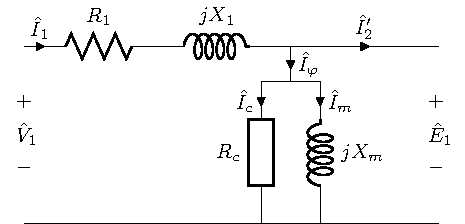
\includegraphics{figTransformersModelSecondPart}
\caption{ٹرانسفارمر مساوی دور، حصہ دوم۔}
\label{شکل_ٹرانسفارمر_ماڈل_حصہ_دوم}
\end{figure}

\جزوحصہ{ثانوی لچھے کی امالی برقی دباؤ}
مرکز میں مشترکہ مقناطیسی بہاؤ ثانوی لچھے میں امالی برقی دباؤ \عددیء{\hat{E}_2} پیدا کرے گی اور چونکہ یہی مقناطیسی بہاؤ ابتدائی لچھے میں \عددیء{\hat{E}_1}  امالی پیدا کرتی ہے لہٰذا
\begin{align}
\frac{\hat{E}_1}{\hat{E}_2}=\frac{N_1}{N_2}
\end{align}
	گزشتہ دو مساواتوں یعنی  اور  کو ایک کامل ٹرانسفارمر سے ظاہر کیا جا سکتا ہے۔ یہ شکل \حوالہ{شکل_ٹرانسفارمر_ماڈل_حصہ_ثوم}  میں دکھایا گیا ہے۔
\begin{figure}
\centering
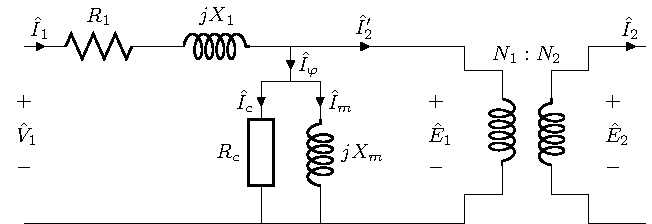
\includegraphics{figTransformersModelThirdPart}
\caption{ٹرانسفارمر مساوی دور، حصہ ثوم۔}
\label{شکل_ٹرانسفارمر_ماڈل_حصہ_ثوم}
\end{figure}

\جزوحصہ{ثانوی لچھے کی مزاحمت اور متعاملہ کے اثرات}
ثانوی لچھے کے سروں پر البتہ  \عددیء{\hat{E}_2} برقی دباؤ نہیں ہوگا چونکہ ثانوی لچھے کے، بالکل ابتدائی لچھے کی طرح، مزاحمت \عددیء{R_2}  اور متعاملہ  \عددیء{j X_2} ہوں گے جن میں ثانوی برقی رو \عددیء{\hat{I}_2}  کی وجہ سے برقی دباؤ گھٹے گا۔  لہٰذا ثانوی لچھے کے سروں پر برقی دباؤ \عددی{\hat{V}_2} قدرِ کم ہو گا۔ یعنی
\begin{align}
\hat{V}_2=\hat{E}_2-\hat{I}_2 R_2-j \hat{I}_2 X_2
\end{align}
	یوں حاصل ٹرانسفارمر کا مکمل مساوی دور شکل  \حوالہ{شکل_ٹرانسفارمر_مکمل_ماڈل} میں دکھایا گیا ہے۔
\begin{figure}
\centering
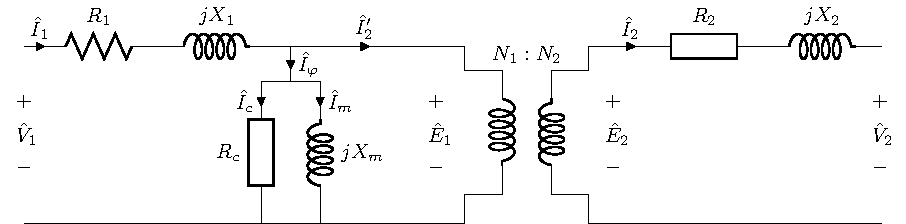
\includegraphics[width=0.9\linewidth]{figTransformersModelComplete}
\caption{ٹرانسفارمر کا مکمل مساوی دور۔}
\label{شکل_ٹرانسفارمر_مکمل_ماڈل}
\end{figure}

\جزوحصہ{مقاومت کا ابتدائی یا ثانوی جانب تبادلہ}
شکل \حوالہ{شکل_ٹرانسفارمر_مکمل_ماڈل}  میں دکھائے دور کے سب جز کا تبادلہ ایک جانب سے دوسری جانب کیا جا سکتا ہے۔ یہ کرنے سے کامل ٹرانسفارمر کو مساوی دور کی بائیں یا دائیں جانب لے جایا جا سکتا ہے۔شکل \حوالہ{شکل_ٹرانسفارمر_مکمل_ماڈل_ابتدائی_جانب}   میں ثانوی جانب کی مقاومت کا ابتدائی جانب تبادلہ کیا گیا ہے جبکہ شکل  \حوالہ{شکل_ٹرانسفارمر_مکمل_ماڈل_ثانوی_جانب}  میں ابتدائی جانب کی مقاومت کا ثانوی جانب تبادلہ کیا گیا ہے۔اس طرح حاصل مساوی دور میں عموما ً کامل ٹرانسفارمر بنایا ہی نہیں جاتا۔یہی شکل \حوالہ{شکل_ٹرانسفارمر_مکمل_ماڈل_ثانوی_جانب}   میں کیا گیا ہے۔

تبادلہ شدہ مقاومت  \عددیء{Z} کو \عددیء{Z'}  سے ظاہر کیا جاتا ہے۔یوں \عددیء{R_2} کے ٹرانسفارمر کی دوسری جانب تبادلہ کے بعد اسے \عددیء{R_2'} سے ظاہر کیا گیا ہے۔

ایسا دور استعمال کرتے وقت یہ ذہن میں رکھنا ہوتا ہے کہ ٹرانسفارمر کے کس جانب دور حل کیا جا رہا ہے۔
\begin{figure}
\centering
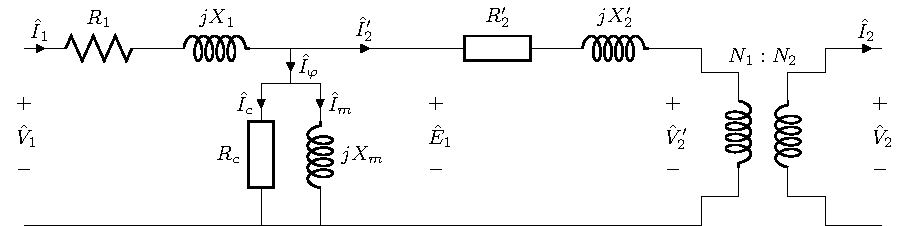
\includegraphics[width=0.9\linewidth]{figTransformersModelShiftedToPrimarySide}
\caption{ثانوی جانب  مقاومت کا ابتدائی جانب تبادلہ کیا گیا ہے۔}
\label{شکل_ٹرانسفارمر_مکمل_ماڈل_ابتدائی_جانب}
\end{figure}
%
\begin{figure}
\centering
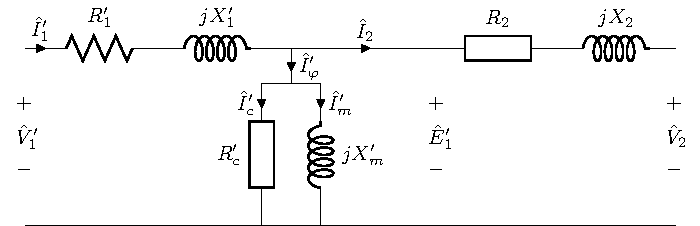
\includegraphics[width=0.9\linewidth]{figTransformersModelShiftedToSecondarySide}
\caption{ابتدائی جانب مقاومت کا ثانوی جانب تبادلہ کیا گیا ہے۔}
\label{شکل_ٹرانسفارمر_مکمل_ماڈل_ثانوی_جانب}
\end{figure}


%
\ابتدا{مثال}
ایک \عددیء{50} کلو وولٹ-ایمپیئر اور  \عددیء{2200:220} وولٹ برقی اہلیت کے ٹرانسفارمر کی زیادہ برقی دباؤ کی جانب کی رستا مقاومت \عددیء{Z_1=0.9+j 1.2}  اوہم اور کم برقی دباؤ کی جانب کی رِستا مقاومت \عددیء{Z_2=0.0089+j 0.011} اوہم ہے۔اگر اس کی \عددیء{R_c=\SI{6.4}{\ohm}} اور \عددیء{X_m=\SI{47}{\ohm}}  ہو تو اس کی شکل  اور شکل  میں استعمال ہونے والے جُز معلوم کریں۔

	حل حصہ اول:
معلومات:
\begin{align*}
\SI{50}{\kilo \volt \ampere}, \quad \SI{50}{\hertz}, \quad 2200:220\,\textup{V}
\end{align*}
ٹرانسفارمر کے دونوں جانب کی برقی دباؤ لچھوں کے چکروں کی نسبت سے ہوتے ہیں لہٰذا
\begin{align*}
\frac{N_1}{N_2}=\frac{2200}{220}=\frac{10}{1}
\end{align*}
یوں اگر ٹرانسفارمر کی مقاومت کا زیادہ برقی دباؤ کی جانب تبادلہ کیا جائے تو
\begin{align*}
R_2'+j X_2' &=\left(\frac{N_1}{N_2} \right)^2 \left(R_2+j X_2 \right)\\
&=\left(\frac{10}{1} \right)^2 \left(0.0089+j 0.011 \right)\\
&=0.89+j 1.1
\end{align*}
جبکہ اس کی بقایا مقاومت وہی رہیں گے۔یوں شکل  کے جُز حاصل ہوئے۔

	حل حصہ دوم:
اگر مساوی دور کی مقاومت کا کم برقی دباؤ کی جانب تبادلہ کیا جائے تب
\begin{align*}
R_1'+j X_1' &=\left(\frac{N_2}{N_1} \right)^2 \left(R_1+j X_1 \right)\\
&=\left(\frac{1}{10} \right)^2 \left(0.9+j1.2 \right)\\
&=0.009+j0.012
\end{align*}
اسی طرح
\begin{align*}
R_c'&=\left(\frac{N_2}{N_1} \right) R_c=0.064\\
X_m'&=\left(\frac{N_2}{N_1} \right) X_m=0.47
\end{align*}
جبکہ \عددیء{Z_2} وہی رہے گا۔
\انتہا{مثال}
%
\جزوحصہ{ٹرانسفارمر کے سادہ ترین مساوی دور}
ایک انجنیئر کو جب ایک ٹرانسفارمر استعمال کرنا ہو تو وہ حساب کرتے وقت شکل  میں دیئے گئے دور کو استعمال کر سکتا ہے۔ یہ دور حقیقی ٹرانسفارمر کی بہت اچھی عکاسی کرتا ہے۔ البتہ جہاں ہمیں نہایت صحیح جواب مطلوب نہ ہوں وہاں اس دور کی سادہ اشکال بھی استعمال کی جا سکتیں ہیں۔ اس باب میں ہم ایسے ہی سادہ مساوی دوروں کا ذکر کریں گے۔
\begin{figure}
\centering
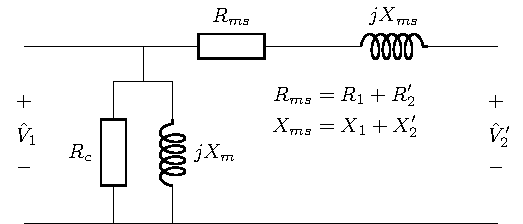
\includegraphics[width=0.9\linewidth]{figTransformersModelLeftHand}
\caption{\عددیء{R_c} اور \عددیء{jX_m} کو بائیں جانب منتقل کیا گیا ہے۔}
\label{شکل_ٹرانسفارمر_بائیں_جانب}
\end{figure}
%
\begin{figure}
\centering
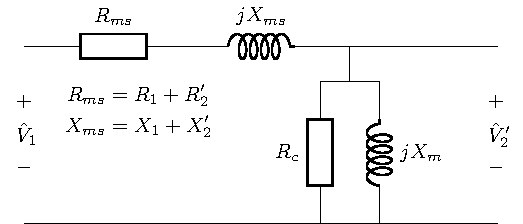
\includegraphics[width=0.9\linewidth]{figTransformersModelRightHand}
\caption{\عددیء{R_c} اور \عددیء{jX_m} کو دائیں جانب منتقل کیا گیا ہے۔}
\label{شکل_ٹرانسفارمر_دائیں_جانب}
\end{figure}

شکل  \حوالہ{شکل_ٹرانسفارمر_مکمل_ماڈل_ابتدائی_جانب} میں \عددیء{R_c} اور \عددیء{X_m} کو بائیں یا دائیں طرف لے جانے سے  شکل  \حوالہ{شکل_ٹرانسفارمر_بائیں_جانب}  اور  شکل \حوالہ{شکل_ٹرانسفارمر_دائیں_جانب}  حاصل ہوتے ہیں۔چونکہ \عددیء{\hat{I}_\varphi} کی مقدار نہایت کم\حاشیہد{\عددیء{\hat{I}_\varphi} ٹرانسفارمر کے کُل برقی بار کے صرف دو سے چھ فی صد ہوتی ہے}  ہوتی ہے اس لئے ایسا  کرنے سے حاصل جواب پر کوئی خاص فرق نہیں پڑتا۔ چونکہ اس شکل میں \عددیء{R_1} ،\عددیء{R_2'}، \عددیء{X_1}  اور \عددیء{X_2'} سلسلہ وار ہیں اس لئے ان کو جمع کیا جا سکتا ہے شکل میں ان کو مساوی مزاحمت \عددیء{R_{ms}}  اور مساوی متعاملہ \عددیء{X_{ms}} کہا گیا ہے۔اسی قسم کے ادوار  شکل  \حوالہ{شکل_ٹرانسفارمر_مکمل_ماڈل_ثانوی_جانب} سے بھی حاصل ہوتے  ہیں۔

ہم ایک قدم اور آگے جا سکتے ہیں اور \عددیء{\hat{I}_\varphi} کو مکمل طور پر نظر انداز کر سکتے ہیں یعنی اس کو ہم صفر تصور کر لیتے ہیں۔اس کا مطلب ہے کہ مساوی دور میں \عددیء{R_c} اور \عددیء{j X_m} دونوں کو کھلے دور کیا جاتا ہے  یعنی انہیں مساوی دور سے ہٹا دیا جاتا ہے۔ شکل \حوالہ{شکل_ٹرانسفارمر_سادہ_ماڈل}-الف  میں یہ دکھائے گئے ہیں۔اس دور میں مرکز کے اثرات کو مکمل طور پر نظرانداز کیا گیا ہے۔

بیشتر وقت ہمیں اس سے بھی کم صحیح جواب مطلوب ہوتا ہے۔چونکہ \عددیء{X_m\gg R_c}  لہٰذا ہم  \عددیء{R_{ms}} کو بھی نظرانداز کر سکتے ہیں۔یوں شکل \حوالہ{شکل_ٹرانسفارمر_سادہ_ماڈل}-ب حاصل ہوتا ہے۔
\begin{figure}
\centering
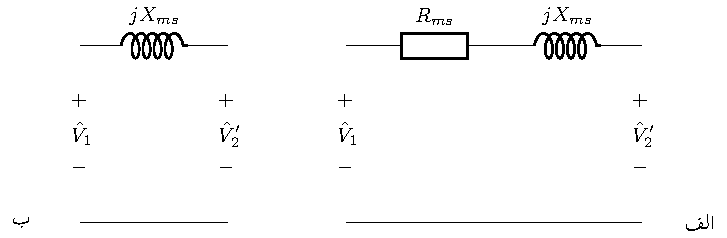
\includegraphics[width=0.9\linewidth]{figTransformersModelCoreLossNeglected}
\caption{ٹرانسفارمر کے سادہ مساوی ادوار۔}
\label{شکل_ٹرانسفارمر_سادہ_ماڈل}
\end{figure}
\حصہ{کھلے دور معائنہ اور کسرِ دور معائنہ}
پچھلے حصے میں بیان کئے گئے ٹرانسفارمر کے مساوی دور کے جُز ٹرانسفارمر کے دو معائنوں سے حاصل کئے جا سکتے ہیں۔ ان معائنوں کو کھلے دور معائنہ اور کسرِ دور معائنہ کہتے ہیں۔اس حصے میں انہیں پر غور کیا جائے گا۔

\جزوحصہ{کھلے دور معائنہ}
کھلے\حاشیہط{یہ حصہ دوبارہ لکھا گیا ہے لہٰذا اشکال پر نظر رکھیں} دور معائنہ\فرہنگ{معائنہ!کھلے دور}\حاشیہب{open circuit test}\فرہنگ{open circuit test} جیسا کہ نام سے واضح  ہے،  ٹرانسفارمر کی ایک جانب لچھے کے سروں کو آزاد رکھ کر کیا جاتا ہے۔ یہ معائنہ اتنی برقی دباؤ اور تعدد یا ان کے قریب ترین مقداروں پر کیا جاتا ہے جتنے پر ٹرانسفارمر کی بناوٹ\فرہنگ{بناوٹ}\حاشیہب{design} ہو۔ اگرچہ یہ معائنہ ٹرانسفارمر کے کسی بھی جانب کے لچھے پر کیا جا سکتا ہے، حقیقت میں اسے کم برقی دباؤ والی جانب کے لچھے پر کرنا آسان ہوتا ہے۔یہ بات ایک مثال سے زیادہ آسانی سے سمجھ آتی ہے۔

	مثلاً  ہم  \عددیء{\SI{25}{\kilo \volt \ampere}} اور \عددیء{11000:220\,\textup{V}}  کا \عددیء{\SI{50}{\hertz}} پر چلنے والے ایک دور کے ٹرانسفارمر کا معائنہ کرنا چاہتے ہیں۔ اگر یہ معائنہ اس کے گیارہ ہزار کے لچھے پر  کیا جائے تو گیارہ ہزار برقی دباؤ کے لگ بھگ برقی دباؤ استعمال کیا جائے گا اور اگر دو سو بیس برقی دباؤ والے لچھے پر کیا جائے تو دو سو بیس برقی دباؤ کے لگ بھگ برقی دباؤ  استعمال کیا جائے گا۔ دونوں صورتوں میں تعدد \عددیء{\SI{50}{\hertz}} کے لگ بھگ رکھا جائے گی۔\عددیء{\SI{11}{\kilo \volt}} کی برقی دباؤ پر کام کرنا نہایت خطرناک ثابت ہو سکتا ہے۔یہی وجہ ہے کہ اس معائنہ کو کم برقی دباؤ والے لچھے پر ہی کیا جاتا ہے۔

 جس برقی دباؤ پر ٹرانسفارمر عام حالات میں استعمال ہوتا ہے اس معائنہ میں کم برقی دباؤ والی جانب کے لچھے پر اتنے ہی یا اس کی قریب مقدار کی برقی دباؤ \عددیء{V_t} لاگو کر کے کھلے دور برقی طاقت \عددیء{p_t} اور  کھلے دور برقی رو \عددیء{I_t}  ناپے جاتے ہیں۔معائنہ حقیقت میں استعمال کے دوران برقی دباؤ کے جتنے قریب برقی دباؤ پر کیا جائے اتنا بہتر جواب حاصل ہوتا ہے۔ ٹرانسفارمر کی دوسری جانب لچھے کے سرے چونکہ آزاد رکھے جاتے ہیں اس لئے اس میں  برقی رو صفر ہوگا۔  لہٰذا ناپا گیا برقی رو صرف ہیجان انگیز برقی رو \عددیء{\hat{I}_\varphi} ہوگا۔ ٹرانسفارمر جتنی برقی رو کے لئے بنایا گیا ہو یہ برقی رو اس  کے تقریباً دو سے چھ  فیصد ہوتا ہے۔شکل \حوالہ{شکل_ٹرانسفارمر_مکمل_ماڈل_ابتدائی_جانب}   کو مدِ نظر رکھتے ہوئے اگر ہم بائیں جانب کو کم برقی دباؤ والی جانب تصور کریں تو شکل میں \عددیء{V_t} کو  \عددیء{V_1} کی جگہ لاگو کرنا ہو گا۔یوں ہم جو برقی رو ناپیں گے وہ  مقداری\حاشیہب{scalar} \عددیء{I_1}  ہو گا۔ چونکہ  \عددیء{I_2'} صفر کے برابر ہے لہٰذا \عددیء{I_1}  درحقیقت \عددیء{\hat{I}_\varphi} کے مقدار \عددیء{I_\varphi} کے برابر ہوگا۔ یعنی  اس  طرح
\begin{align*}
I_t=I_1=I_\varphi
\end{align*}
اتنی کم برقی رو سے لچھے کی مقاومت میں نہایت کم برقی دباؤ گھٹتا ہے،لہٰذا اسے نظر انداز کیا جاتا ہے یعنی
\begin{align*}
V_{R1}&=I_t R_1=I_\varphi R_1 \approx 0\\
V_{X1}&=I_1 X_1=I_\varphi X_1 \approx 0
\end{align*}
یوں  \عددیء{R_c}  اور \عددیء{X_m} پر  تقریباً \عددیء{V_t} برقی دباؤ پایا جائے گا۔ یہ شکل \حوالہ{شکل_ٹرانسفارمر_مکمل_ماڈل_ابتدائی_جانب}  سے ظاہر ہے۔ان حقائق کو مد نظر رکھتے ہوئے شکل \حوالہ{شکل_ٹرانسفارمر_کھلے_سرے_معائنہ} حاصل ہوتا ہے۔
\begin{figure}
\centering
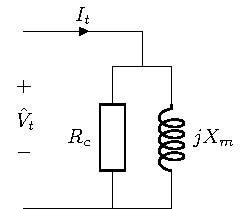
\includegraphics{figTransformersOpenCircuitTest}
\caption{کھلے سِرے معائنہ۔}
\label{شکل_ٹرانسفارمر_کھلے_سرے_معائنہ}
\end{figure}

چونکہ برقی طاقت کا ضیاع صرف مزاحمت میں ہی ممکن ہے لہٰذا \عددیء{p_t} صرف  \عددیء{R_c}  میں ہی ضائع ہو گی۔ یوں
\begin{align*}
p_t=\frac{V_t^2}{R_c}
\end{align*}
لکھا جائے گا۔یوں
\begin{align}\label{مساوات_ٹرانسفارمر_کھلے_دور_مزاحمت_حاصل}
R_c&=\frac{V_t^2}{p_t}
\end{align}
حاصل ہوتا ہے۔

اسی طرح چونکہ برقی دباؤ اور برقی رو کی مقداروں کے تناسب کو مقاومت کی مقدار کہتے ہیں لہٰذا
\begin{align*}
\abs{Z_t}=\frac{V_t}{I_t}
\end{align*}
مگر شکل  سے واضح ہے کہ
\begin{align*}
\frac{1}{Z_t}=\frac{1}{R_c}+\frac{1}{j X_m}
\end{align*}
لہٰذا
\begin{align*}
Z_t&=\frac{j R_c X_m}{R_c+j X_m}\\
\abs{Z_t}&=\frac{R_c X_m}{\sqrt{R_c^2+X_m^2}}
\end{align*}
جس سے حاصل ہوتا ہے
\begin{align}\label{مساوات_ٹرانسفارمر_کھلے_دور_امالہ_حاصل}
X_m=\frac{R_c \abs{Z_t}}{\sqrt{R_c^2-\abs{Z_t}^2}}
\end{align}
مساوات \حوالہ{مساوات_ٹرانسفارمر_کھلے_دور_مزاحمت_حاصل}  سے \عددیء{R_c} اور  مساوات \حوالہ{مساوات_ٹرانسفارمر_کھلے_دور_امالہ_حاصل}  سے  \عددیء{X_m}  کا حساب لگایا جاتا ہے۔

یاد رہے کہ حاصل کردہ \عددیء{R_c} اور \عددیء{X_m} ٹرانسفارمر کے اسی جانب کے لئے درست ہیں جس جانب انہیں حاصل کیا گیا ہو۔اگر ان کی قیمتیں دوسری جانب درکار ہوں تب تبادلہ مقاومت کا استعمال کرتے ہوئے اس جانب کی قیمتیں حاصل کی جا سکتی ہیں۔ 

\جزوحصہ{ کسرِ دور معائنہ}
یہ معائنہ بھی پچھلے معائنہ کی طرح ٹرانسفارمر کے کسی بھی طرف کیا جا سکتا ہے مگر حقیقت میں اسے زیادہ برقی دباؤ کے لچھے پر ہی کرنا زیادہ آسان ہوتا ہے۔ یہ معائنہ جتنے برقی رو کے لئے ٹرانسفارمر بنایا گیا ہو اتنی برقی رو یا اس کے قریب مقدار پر کیا جاتا ہے۔یعنی اس معائنہ میں کوشش ہوتی ہے کہ ٹرانسفارمر کے لچھے میں اتنی برقی رو گزرے جتنی کے لئے یہ بنایا گیا ہو۔ لہٰذا اگر ہم پچھلے معائنہ میں استعمال ہونے والے ٹرانسفارمر کی بات آگے بڑھائیں تو اس کا زیادہ برقی دباؤ کا لچھا \عددیء{\SI{2.2727}{\ampere}} اور کم برقی دباؤ کا لچھا \عددیء{\SI{113.63}{\ampere}} کے لئے بنایا گیا ہے۔ لہٰذا اگر یہ معائنہ کم برقی دباؤ لچھے پر کیا جائے تو اسے \عددیء{\SI{113.63}{\ampere}}  پر  کرنا ہوگا اور اگر زیادہ برقی دباؤ لچھے پر کیا جائے تو صرف \عددیء{\SI{2.2727}{\ampere}} پر کرنا ہوگا جو کہ زیادہ آسان ہے۔
\begin{figure}
\centering
\includegraphics{figTransformersShortCircuitTest}
\caption{کسر دور معائنہ۔}
\label{شکل_ٹرانسفارمر_کسر_دور_معائنہ}
\end{figure}

اس معائنہ میں کم برقی دباؤ لچھے کے دونوں سروں کو آپس میں جوڑا جاتا ہے یعنی انہیں کسرِ دور کر لیا جاتا ہے اور زیادہ برقی دباؤ لچھے پر اس جانب کی ڈیزائن کردہ برقی دباؤ کے دو سے بارہ  فی صد کا برقی دباؤ \عددیء{V_t} لاگو کر کے کسرِ دور برقی رو \عددیء{I_t} اور کسرِ دور برقی طاقت \عددیء{p_t} ناپے جاتے ہیں۔ جس لچھے کے سرے آپس میں کسرِ دور ہوتے ہیں اس میں سے برقی رو گزرتی ہے اور اس کا عکس دوسری جانب بھی موجود ہوتا ہے۔ یہ برقی رو ٹرانسفارمر کے ڈیزائن کردہ برقی رو کے لگ بھگ ہوتا ہے۔ اس معائنہ کا دور شکل \حوالہ{شکل_ٹرانسفارمر_کسر_دور_معائنہ} میں دکھایا گیا ہے۔کھلے سرے معائنے کی طرح اگر کسر دور معائنے میں بھی  شکل \حوالہ{شکل_ٹرانسفارمر_مکمل_ماڈل_ابتدائی_جانب} کے بائیں جانب کو کم برقی دباؤ والی جانب تصور کریں تو  \عددیء{V_t} کو  \عددیء{V_2} کی جگہ لاگو کرنا ہو گا۔

 چونکہ یہ معائنہ بہت کم برقی دباؤ پر کیا جاتا ہے لہٰذا اس معائنہ میں ہیجان انگیز برقی رو کو مکمل طور پر نظرانداز کیا جا سکتا ہے۔ شکل سے ہم دیکھتے ہیں کہ چونکہ برقی طاقت صرف مزاحمت میں ہی ضائع ہو سکتی ہے لہٰذا
\begin{align*}
p_t=I_t^2 \left(R_{ms}\right)
\end{align*}
ہو گا جس سے
\begin{align}\label{مساوات_ٹرانسفارمر_کسر_دور_مزاحمت_حاصل}
R_{ms}=\frac{p_t}{I_t^2}
\end{align}
حاصل ہوتا ہے۔

کسرِ دور برقی رو اور برقی دباؤ سے ہمیں ملتی ہے
\begin{align*}
\abs{Z_t}=\frac{V_t}{I_t}
\end{align*}
مگر شکل سے واضح ہے کہ
\begin{align*}
Z_t&=R_{ms}+j X_{ms}\\
\abs{Z_t}&=\sqrt{R_{ms}^2+X_{ms}^2}
\end{align*}
لہٰذا
\begin{align}\label{مساوات_ٹرانسفارمر_کسر_دور_امالہ_حاصل}
X_{ms}=\sqrt{\abs{Z_t}^2-R_{ms}^2}
\end{align}
مساوات \حوالہ{مساوات_ٹرانسفارمر_کسر_دور_مزاحمت_حاصل} کُل مزاحمت دیتا ہے البتہ اس سے \عددی{R_1} یا \عددیء{R_2} حاصل نہیں کیا جا سکتا۔اسی طرح مساوات \حوالہ{مساوات_ٹرانسفارمر_کسر_دور_امالہ_حاصل} سے \عددیء{X_1} اور \عددیء{X_2} علیحدہ نہیں کئے جا سکتے۔کسر دور معائنہ سے اتنی ہی معلومات حاصل کرنا ممکن ہے۔حقیقت میں اتنی معلومات کافی ہوتی ہے۔ اگر ان اجزاء ک علیحدہ علیحدہ قیمتیں درکار ہوں تو ایسی صورت میں تصور کیا جاتا ہے کہ
\begin{align*}
R_1'&=R_2\\
X_1'&=X_2
\end{align*}
ہیں۔

 چونکہ یہ معائنہ عموما ًجہاں ٹرانسفارمر موجود ہو وہیں کرنا پڑتا ہے لہٰذا یہ ممکن نہیں ہوتا کہ ٹرانسفارمر کو بالکل اتنا برقی دباؤ دیا جائے جتنا درکار ہو بلکہ جو برقی دباؤ موجود ہو اسی سے کام چلانا پڑتا ہے۔ لیکن اس بات کا خیال بہت ضروری ہے کہ جو برقی دباؤ ٹرانسفارمر کو دیا جا رہا ہو وہ ڈیزائن کردہ برقی دباؤ کے دو سے بارہ  فی صد ہو۔ مثلاً اگر اسی \عددیء{11000:220\,\textup{V}} ٹرانسفارمر کی بات کی جائے تو اس کے زیادہ برقی دباؤ لچھے پر \عددیء{\SI{220}{\volt}} اور \عددیء{\SI{1320}{\volt}}  کے درمیان کوئی بھی برقی دباؤ دیا جا سکتا ہے۔ چونکہ ہمارے ہاں \عددیء{\SI{220}{\volt}}  اور \عددیء{\SI{440}{\volt}}  عام پائے جاتے ہیں لہٰذا ہم \عددیء{\SI{220}{\volt}}  یا \عددیء{\SI{440}{\volt}}  ہی استعمال کریں گے۔

یہاں یہ ایک مرتبہ دوبارہ یاد دھیانی کراتا جاؤں کہ ٹرانسفارمر کی ایک جانب لچھے کے سرے آپس میں جوڑ کر، یعنی انہیں کسرِ دور کر کے، دوسری جانب لچھے پر کسی بھی صورت میں اس جانب کی پوری برقی دباؤ لاگو نہیں کرنا۔ ایسا کرنا  شدید  خطرناک اور جان لیوا ثابت ہو سکتا ہے۔

یاد رہے کہ حاصل کردہ \عددیء{R_c} اور \عددیء{X_m} ٹرانسفارمر کے اسی جانب کے لئے درست ہیں جس جانب انہیں حاصل کیا گیا ہو۔اگر ان کی قیمتیں دوسری جانب درکار ہوں تب تبادلہ مقاومت کا استعمال کرتے ہوئے اس جانب کی قیمتیں حاصل کی جا سکتی ہیں۔ 
%
\ابتدا{مثال}
ایک \عددیء{25}  کلو وولٹ-ایمپیئر، \عددیء{11000:220} وولٹ اور \عددیء{50} ہرٹز پر چلنے والے ٹرانسفارمر کے کھلے دور اور کسرِ دور معائنہ کئے جاتے ہیں جن کے نتائج یہ ہیں۔
\begin{itemize}
\item
کھلے دور معائنہ کرتے وقت کم برقی دباؤ کی جانب  \عددیء{\SI{220}{\volt}} لاگو کئے جاتے ہیں۔اسی جانب برقی رو \عددیء{\SI{39.64}{\ampere}} اور طاقت کا ضیاع \عددیء{\SI{600}{\watt}} ناپے جاتے ہیں۔
\item
کسرِ دور معائنہ کرتے وقت زیادہ برقی دباؤ کی جانب  \عددیء{\SI{440}{\volt}} لاگو کئے جاتے ہیں۔اسی جانب برقی رو \عددیء{\SI{2.27}{\ampere}} اور طاقت کا ضیاع \عددیء{\SI{560}{\watt}} ناپے جاتے ہیں۔
\end{itemize}

کھلے دور حل:
\begin{align*}
\abs{Z_t}&=\frac{220}{39.64}=\SI{5.55}{\ohm}\\
R_c&=\frac{220^2}{600}=\SI{80.67}{\ohm}\\
X_m&=\frac{80.67 \times 5.55}{\sqrt{80.67^2-5.55^2}}=\SI{5.56}{\ohm}
\end{align*}
کسر دور حل:
\begin{align*}
Z_t&=\frac{440}{2.27}=\SI{193.83}{\ohm}\\
R_{ms}&=\frac{560}{2 \times 2.27^2}=\SI{108.68}{\ohm}\\
X_{ms}&=\sqrt{193.83^2-108.68^2}=\SI{160}{\ohm}
\end{align*}

ان نتائج کو کم برقی دباو جانب منتقل کرتے ہوئے 
\begin{align*}
\left(\frac{220}{11000} \right)^2 \times 108.68=\SI{43.47}{\milli \ohm}\\
\left(\frac{220}{11000} \right)^2 \times 160=\SI{64}{\milli \ohm}
\end{align*}
یعنی
\begin{align*}
R_1&=R_2'=\frac{\SI{43.47}{\milli \ohm}}{2}=\SI{21.7}{\milli \ohm}\\
X_1&=X_2'=\frac{\SI{64}{\milli \ohm}}{2}=\SI{32}{\milli \ohm}
\end{align*}
حاصل ہوتا ہے۔ان نتائج سے حاصل کم برقی دباو جانب مساوی دور شکل \حوالہ{شکل_ٹرانسفارمر_کھلے_سرے_کسر_دور_مثال} میں دکھایا گیا ہے۔
\begin{figure}
\centering
\includegraphics{figTransformersOpenAndShortTestExample}
\caption{کھلے دور اور کسرِ دور معائنہ سے کم برقی دباو جانب  مساوی دور۔}
\label{شکل_ٹرانسفارمر_کھلے_سرے_کسر_دور_مثال}
\end{figure}
\انتہا{مثال}
%
\حصہ{تین دور کے ٹرانسفارمر}
اب تک ہم ایک دور کے ٹرانسفارمر پر غور کرتے رہے ہیں۔حقیقت میں برقی طاقت کی منتقلی میں عموما ً تین دور کے ٹرانسفارمر استعمال ہوتے ہیں۔تین دور کا ٹرانسفارمر عام ایک دور کے تین یکساں ٹرانسفارمر اکٹھے رکھ کر بنایا جا سکتا ہے۔یوں اگر ایک ٹرانسفارمر خراب ہو جائے تو اس کو ٹھیک ہونے کے لئے ہٹا کر بقایا دو ٹرانسفارمر دوبارہ چالو کئے جا سکتے ہیں۔تین دور ٹرانسفارمر بنانے کا اس سے بہتر طریقہ شکل \حوالہ{شکل_ٹرانسفارمر_ایک_مرکز_تین-ٹرانسفارمر} میں دکھایا گیا ہے جہاں ایک ہی مقناطیسی مرکز پر تینوں ٹرانسفارمر کے لچھے لپٹے گئے ہیں۔اس شکل میں \عددیء{\hat{V}_{i1}} پہلے ٹرانسفارمر کا ابتدائی لچھا جبکہ \عددیء{\hat{V}_{s1}} اس کا ثانوی لچھا ہے۔اس طرح کے تین دور کے ٹرانسفارمر سستے، ہلکے اور چھوٹے ہونے کی وجہ سے عام ہو گئے ہیں اور آپ کو روز مرہ زندگی میں یہی نظر آئیں گے۔ان میں برقی ضیاع بھی قدرِ کم ہوتی ہے۔
\begin{figure}
\centering
\includegraphics{figTransformersThreePhaseSingleCore}
\caption{ایک ہی مرکز پر تین ٹرانسفارمر۔}
\label{شکل_ٹرانسفارمر_ایک_مرکز_تین-ٹرانسفارمر}
\end{figure}

شکل  الف میں تین ٹرانسفارمر دکھائے گئے ہیں۔ان تین ٹرانسفارمر کے ابتدائی لچھے آپس میں دو طریقوں سے جوڑے جا سکتے ہیں۔ایک کو ستارا نما جوڑ\فرہنگ{ستارا نما جوڑ}\فرہنگ{جوڑ!ستارا نما}\حاشیہب{star connected}\فرہنگ{star connected} \عددیء{Y}  اور دوسرے کو تکونی جوڑ\فرہنگ{تکونی جوڑ}\فرہنگ{جوڑ!تکونی}\حاشیہب{delta connected}\فرہنگ{delta connected}  \عددیء{\Delta}   کہتے ہیں۔اسی طرح ان تینوں ٹرانسفارمروں کے ثانوی  لچھے انہیں دو طریقوں سے جوڑے جا سکتے ہیں۔یوں انہیں جوڑنے کے چار ممکنہ طریقے ہیں یعنی
\begin{itemize}
\item
ستارا:تکونی  \quad \عددیء{Y:\Delta}
\item
ستارا:ستارا \quad  \عددیء{Y:Y}
\item
تکونی:تکونی \quad  \عددیء{\Delta:\Delta}
\item
تکونی:ستارا  \quad  \عددیء{\Delta:Y}
\end{itemize}

شکل \حوالہ{شکل_ٹرانسفارمر_ستارہ_تکونی_جوڑ}-الف میں ان تین ٹرانسفارمروں کے ابتدائی لچھوں کو ستارا نما جوڑا گیا ہے جبکہ ان کی ثانوی لچھوں کو تکونی جوڑا گیا ہے۔شکل-ب میں تینوں ٹرانسفارمر کی ابتدائی لچھوں کو  ستارہ نما  دکھایا گیا ہے۔اسی طرح ثانوی لچھوں کو تکونی  دکھایا گیا ہے۔انہی شکلوں کی وجہ سے ان کو ستارا نما جوڑ اور تکونی جوڑ کہتے ہیں۔

ایسی شکل بناتے وقت تینوں ٹرانسفارمروں کے ابتدائی لچھے کو جس زاویہ پر بنایا جاتا ہے اس کے ثانوی لچھے کو بھی اُسی زاویہ پر بنایا جاتا ہے۔یوں شکل کے حصہ الف میں سب سے اوپر ٹرانسفارمر جس کے ابتدائی جانب کے  سِرے \عددیء{an} اور ثانوی جانب  کے سِرے \عددیء{a'n'} ہیں کو حصہ با میں صفر زاویہ پر بنایا گیا ہے۔تین دور کے ٹرانسفارمروں کو اس طرح کی علامتوں سے ظاہر کیا جاتا ہے اور ان میں مرکز نہیں دکھایا جاتا۔

ٹرانسفارمر کے جوڑ بیان کرتے وقت بائیں جانب کے جوڑ کو پہلے اور دائیں جانب کی جوڑ کو بعد میں پکارتے ہیں۔یوں شکل میں ٹرانسفارمر کو ستارا-تکونی جُڑا ٹرانسفارمر کہیں گے۔اسی طرح ابتدائی جانب کو بائیں اور ثانوی جانب کو دائیں ہاتھ بنایا جاتا ہے۔یوں اس شکل میں ابتدائی جانب ستارا نما ہے جبکہ ثانوی جانب تکونی ہے۔
\begin{figure}
\centering
\includegraphics[width=\linewidth]{figTransformersStarDeltaConnections}
\caption{تین دور کا ستارہ-تکونی ٹرانسفارمر}
\label{شکل_ٹرانسفارمر_ستارہ_تکونی_جوڑ}
\end{figure}


	ستارا نما جڑی جانب سے چار برقی تاریں نکلتی ہیں۔اس جانب لچھوں کے مشترکہ سِرا \عددیء{n} کو عموما ً ٹرانسفارمر کے نزدیک زمین میں گہرائی تک دھنسا دیا جاتا ہے۔اس تار کو زمینی تار\فرہنگ{زمینی تار}\حاشیہب{ground}\فرہنگ{ground wire}  یا صرف زمین\فرہنگ{زمین}\حاشیہب{ground, earth,neutral}\فرہنگ{earth}  کہتے ہیں۔عام فہم میں اسے ٹھنڈی تار\فرہنگ{ٹھنڈی تار}\حاشیہب{neutral} کہتے ہیں۔باقی تین یعنی \عددیء{a,b,c}  گرم تار\فرہنگ{گرم تار}\حاشیہب{live wires} کہلاتے ہیں۔

ٹرانسفارمر کی لچھے پر برقی دباؤ کو دوری برقی دباؤ\فرہنگ{دوری برقی دباؤ} \عددیء{\hat{V}_{\textup{دور}}}\حاشیہب{phase voltage}\فرہنگ{phase voltage} کہتے ہیں اور لچھے میں برقی رو کو دوری برقی رو\فرہنگ{دوری برقی رو} \عددیء{\hat{I}_{\textup{دور}}}\حاشیہب{phase current}\فرہنگ{phase current}  کہتے ہیں۔ جبکہ ٹرانسفارمر سے باہر نکلتی کسی دو گرم تاروں کے مابین برقی دباؤ کو تار کی برقی دباؤ\فرہنگ{تار کی برقی دباؤ} \عددیء{\hat{V}_{\textup{تار}}}\حاشیہب{line to line voltage}\فرہنگ{line voltage} کہتے ہیں اور کسی بھی گرم تار میں برقی رو کو تار کی برقی رو\فرہنگ{تار کی برقی رو} \عددیء{\hat{I}_{\textup{تار}}}\حاشیہب{line current}\فرہنگ{line current}  کہتے ہیں۔ زمینی تار میں برقی رو کو زمینی برقی رو\فرہنگ{زمینی برقی رو}  \عددیء{\hat{I}_{\textup{زمینی}}}\حاشیہب{ground current}\فرہنگ{ground current} کہتے ہیں۔

ستارا نما \عددیء{Y} جانب دوری مقداروں اور تار کی مقداروں  کا آپس میں یوں رشتہ ہے
\begin{gather}
\begin{aligned}
V_{\textup{تار}}&=\sqrt{3} V_{\textup{دور}}\\
I_{\textup{تار}}&=I_{\textup{دور}}
\end{aligned}
\end{gather}
جبکہ تکونی \عددیء{\Delta} جانب دوری اور تار کی مقداروں کا آپس میں یوں رشتہ ہے
\begin{gather}
\begin{aligned}
V_{\textup{تار}}&= V_{\textup{دور}}\\
I_{\textup{تار}}&=\sqrt{3} I_{\textup{دور}}
\end{aligned}
\end{gather}
یہ دوری سمتیہ کے رشتے نہیں بلکہ ان کی مقداری قیمتوں کے رشتے ہیں۔ان دو مساواتوں سے حاصل ہوتا ہے
\begin{align}
V_{\textup{تار}} I_{\textup{تار}}=\sqrt{3} V_{\textup{دور}} I_{\textup{دور}}
\end{align}
چونکہ ایک دور کی ٹرانسفارمر کی وولٹ-ایمپیئر \عددیء{V_{\textup{دور}} I_{\textup{دور}}} ہیں اور ایسے تین ٹرانسفارمر مل کر ایک تین دور کا ٹرانسفارمر بناتے ہیں لہٰذا تین دور کے ٹرانسفارمر کی وولٹ-ایمپیئر اس کے تین گنا ہوں گے یعنی
\begin{align}
\textup{وولٹ-ایمپیئر}= 
3 V_{\textup{دور}} I_{\textup{دور}}= 
3 \times \frac{V_{\textup{تار}} I_{\textup{تار}}}{\sqrt{3}}=
\sqrt{3} V_{\textup{تار}} I_{\textup{تار}}
\end{align}
یہ مساوات تین دور میں عام استعمال ہوتی ہے۔

	ٹرانسفارمر کسی طرح بھی جوڑے جائیں وہ اپنی بنیادی کارکردگی تبدیل نہیں کرتے لہٰذا انہیں ستارا نما یا تکونی جوڑنے کے بعد بھی ان میں ہر ایک ٹرانسفارمر انفرادی طور پر مساوات  اور  پر پورے اترے گا۔انہیں استعمال کر کے شکل  میں دیئے گئے ٹرانسفارمروں کے ابتدائی اور ثانوی جانب کی دوری اور تار کی مقداروں کے رشتے حاصل کئے جا سکتے ہیں۔اس شکل میں \عددیء{a=N_1/N_2} ہے جہاں  \عددیء{N_1:N_2} ان میں ایک دور کی ٹرانسفارمر کے چکر کی نسبت ہے۔تین دور کے ٹرانسفارمر پر لگی تختی پر دونوں جانب تار کی برقی دباؤ کی نسبت لکھی جاتی ہے۔
\begin{figure}
\centering
\includegraphics[width=\linewidth]{figTransformersAllPossibleConnections}
\caption{ابتدائی اور ثانوی جانب تار اور دوری مقداروں کے رشتے۔}
\label{شکل_ٹرانسفارمر_تین_دور_ٹرانسفارمر_کے_مختلف_جوڑ}
\end{figure}


جیسے شکل \حوالہ{شکل_ٹرانسفارمر_تین_دور_ٹرانسفارمر_کے_مختلف_جوڑ} میں دکھایا گیا ہے ستارا-تکونی ٹرانسفارمر کی تار پر برقی دباؤ کی نسبت
\begin{align}
\frac{V_\textup{{ابتدائی}}}{V_\textup{{ثانوی}}}=\sqrt{3} a =\sqrt{3} \left(\frac{N_1}{N_2} \right)
\end{align}
جبکہ ستارا-ستارا کا
\begin{align}
\frac{V_\textup{{ابتدائی}}}{V_\textup{{ثانوی}}}=a =\left(\frac{N_1}{N_2} \right)
\end{align}
تکونی-ستارا کا
\begin{align}
\frac{V_\textup{{ابتدائی}}}{V_\textup{{ثانوی}}}=\frac{a}{\sqrt{3}}=\frac{1}{\sqrt{3}} \left(\frac{N_1}{N_2} \right)
\end{align}
اور تکونی-تکونی کا
\begin{align}
\frac{V_\textup{{ابتدائی}}}{V_\textup{{ثانوی}}}=a =\left(\frac{N_1}{N_2} \right)
\end{align}
ہے۔
%
\ابتدا{مثال}
ایک دور کے تین یکساں ٹرانسفارمروں کو ستارا-تکونی \عددیء{Y:\Delta}  جوڑ کر تین دور کا ٹرانسفارمر بنایا گیا ہے۔ایک دور کے ٹرانسفارمر کی برقی اہلیت درج ذیل ہے:
\begin{align*}
\SI{50}{\kilo \volt \ampere} , \quad 6350:440\,\textup{V}, \quad \SI{50}{\hertz}
\end{align*}
ستارا-تکونی ٹرانسفارمر کی ابتدائی جانب \عددیء{11000}  وولٹ کی تین دوری تار کی برقی دباؤ لاگو کیا گیا۔اس تین دوری ٹرانسفارمر کی ثانوی جانب تار کا برقی دباؤ معلوم کریں۔

حل: حل کرتے وقت ہم ایک دور کے ایک ٹرانسفارمر پر نظر رکھیں گے۔ ابتدائی جانب اگر ایک دور کے ٹرانسفارمر پر غور کیا جائے تو
\begin{align*}
\frac{N_1}{N_2}=\frac{V_1}{V_2}=\frac{6350}{440}
\end{align*}
اور اس پر لاگو برقی دباؤ مساوات  کی مدد سے
\begin{align*}
V_{\textup{ابتدائی، دور}}=\frac{V_{\textup{تار}}}{\sqrt{3}}=\frac{11000}{\sqrt{3}}=\SI{6350.85}{\volt}
\end{align*}
ہے لہٰذا اس ایک دور ٹرانسفارمر کی ثانوی جانب مساوات کی مدد سے
\begin{align*}
V_{\textup{ثانوی}}=\frac{N_2}{N_1} V_{\textup{ابتدائی}}=\frac{440}{6350} \times 6350.85 \approx \SI{440}{\volt}
\end{align*}
ہیں۔چونکہ ثانوی جانب ان تین ٹرانسفارمروں کو تکونی جوڑا گیا ہے لہٰذا مساوات کی مدد سے اس جانب تار کی برقی دباؤ یہی ہو گی۔اس تین دور کے ٹرانسفارمر کی تار پر برقی دباؤ کی نسبت
\begin{align*}
\frac{V_{\textup{ابتدائی، تار}}}{V_{\textup{ثانوی، تار}}}=\frac{11000}{440}
\end{align*}
ہے۔چونکہ ایک دور ٹرانسفارمر \عددیء{50}  کلو وولٹ-ایمپیئر کا ہے لہٰذا یہ تین دوری ٹرانسفارمر  \عددیء{150} کلو وولٹ-ایمپیئر کا ہو گا۔یوں اس تین دور کے ٹرانسفارمر کی اہلیت\فرہنگ{اہلیت}\حاشیہب{rating}\فرہنگ{rating}
\begin{align*}
\SI{150}{\kilo \volt \ampere}, \quad 11000:440\,\textup{V},\quad \SI{50}{\hertz}
\end{align*}
ہوگی۔

	ٹرانسفارمر پر لگی تختی\فرہنگ{تختی}\حاشیہب{name plate}\فرہنگ{name plate} پر اس کی اہلیت بیان ہوتی ہے جس میں ٹرانسفارمر کے دونوں جانب تار کے برقی دباؤ لکھے جاتے ہیں نہ کہ لچھوں کے چکر۔
\انتہا{مثال}
%
ستارا-ستارا جڑے ٹرانسفارمر عام طور استعمال نہیں ہوتے۔اس کی وجہ یہ ہے کہ اگرچہ ان کی تین دور برقی دباؤ  کے بنیادی جُز آپس میں \عددیء{120\degree}  زاویاتی فاصلے پر ہوتے ہیں لیکن ان کی تیسری موسیقائی جُز آپس میں ہم قدم ہوتی ہیں۔مرکز کی غیر بتدریج خصوصیات کی وجہ سے ٹرانسفارمر میں ہر صورت تیسری موسیقائی جُز پائے جاتے ہیں۔تیسری موسیقائی جُز ہم قدم ہونے کی وجہ سے جمع ہو کر ایک نہایت بڑی برقی دباؤ کی موج پیدا کرتے ہیں جو کبھی کبھی برقی دباؤ کی بنیادی جُز سے بھی زیادہ بڑے ہوتے ہیں۔

بقایا تین قسم کے جڑے ٹرانسفارمروں میں برقی دباؤ کی تیسری موسیقائی جُز مسئلہ نہیں کرتیں چونکہ ان میں تکونی جُڑے لچھوں میں برقی رو گردش کرنی شروع ہوجاتی ہے جو ان کے اثر کو ختم کر دیتی ہے۔

تین دور ٹرانسفارمر کے متوازن دور حل کرتے وقت ہم تصور کرتے ہیں کہ ٹرانسفارمر ستارا نما ہے۔یوں اس کے ایک دور میں برقی رو، تار  کی برقی رو ہی ہو گی اور اس کے ایک دور پر لاگو برقی دباؤ، دوری برقی دباؤ  ہو گا۔اسی طرح ہم تصور کرتے ہیں کہ اس پر لدھا برقی بار بھی ستارا نما جُڑا ہے۔یوں تین دور کی جگہ ہم ایک دور کا نسبتاً آسان مسئلہ حل کرتے ہیں۔ ایسا کرنے سے مسئلہ پر غور کرنا آسان ہو جاتا ہے۔یہ ایک مثال سے زیادہ بہتر سمجھ آئے گا۔
%
\ابتدا{مثال}
ایک تین دوری \عددیء{\Delta :Y}   \عددیء{2000} کلو وولٹ-ایمپیئر،  \عددیء{11000:600 }  وولٹ اور \عددیء{50} ہرٹز پر چلنے والا کامل ٹرانسفارمر ایک تین دوری متوازن برقی بار کو طاقت مہیا کر رہا ہے۔یہ بار تکونی جڑا ہے جہاں بار کا ہر حصہ \عددیء{(0.504+j0.1917)} کے برابر ہے۔شکل \حوالہ{شکل_ٹرانسفارمر_تکونی_بار_کی_مثال}  میں یہ دکھایا گیا ہے۔
\begin{itemize}
\item
1. اس شکل میں ہر جگہ برقی رو معلوم کریں۔
\item
2. برقی بار\فرہنگ{بار}\حاشیہب{electrical load}\فرہنگ{load} کو درکار طاقت معلوم کریں
\end{itemize}

\begin{figure}
\centering
\includegraphics[width=\linewidth]{figTransformersDeltaLoadedExample}
\caption{ٹرانسفارمر تکونی متوازن بار کو طاقت فراہم کر رہا ہے۔}
\label{شکل_ٹرانسفارمر_تکونی_بار_کی_مثال}
\end{figure}
حل:

پہلے تکونی بار کو ستارا نما بار میں تبدیل کرتے ہیں
\begin{align*}
Z_Y= \frac{Z_\Delta}{3}=\frac{0.504+j0.1917}{3}=0.168+j0.0639
\end{align*}
اس بار کو ستارا نما جڑا شکل \حوالہ{شکل_ٹرانسفارمر_تکونی_بار_کو_ستارہ_تبادلہ} میں دکھایا گیا ہے۔اس شکل میں ایک برقی تار جسے نقطہ دار لکیر سے ظاہر کیا گیا ہے کو ٹرانسفارمر کی زمینی نقطہ سے بار کے مشترکہ سِرے کے درمیان جڑا دکھایا گیا ہے۔متوازن دور میں اس تار میں برقی رو صفر ہوگی۔حل کرنے کی نیت سے ہم اس متوازن دور سے ایک حصہ لے کر حل کرتے ہیں۔
\begin{figure}
\centering
\includegraphics[width=\linewidth]{figTransformersDeltaLoadedExampleTurnedStar}
\caption{تکونی بار کو مثاوی ستارہ بار میں تبدیل کیا گیا ہے۔}
\label{شکل_ٹرانسفارمر_تکونی_بار_کو_ستارہ_تبادلہ}
\end{figure}

یوں مساوی برقی بار میں برقی رو
\begin{align*}
I=\frac{346.41}{0.168+j0.0639}=1927.262\phase{-20.825\degree}
\end{align*}
ہو گی اور اس ایک حصہ میں طاقت
\begin{align*}
p=346.41 \times 1927.262 \times \cos (-20.825\degree)=\SI{624007}{\watt}
\end{align*}
ہوگی۔ یوں برقی بار کو پوری درکار برقی طاقت اس کے تین گنا ہو گی یعنی \عددیء{\SI{1872}{\kilo \watt}}  اس بار کا جُز طاقت\حاشیہب{power factor} 
\begin{align*}
\cos (-20.825\degree)=0.93467
\end{align*}
ہے۔

	تکونی بار   میں برقی رو \عددیء{1927.262\sqrt{3}=1112.7} ایمپیئر ہو گی۔ ٹرانسفارمر کی ابتدائی جانب برقی تاروں میں برقی رو
\begin{align*}
\left(\frac{600}{11000} \right) \times 1927.262=105.12
\end{align*}
  ایمپیئر ہو گی۔
\انتہا{مثال}
%
اس مثال میں جُز طاقت \عددیء{0.93467} ہے۔اس کتاب کے لکھتے وقت پاکستان میں اگر صنعتی کارخانوں کی برقی بار کی جُز طاقت \عددیء{0.9} سے کم ہو جائے تو برقی طاقت فراہم کرنے والا ادارہ جرمانہ نافذ کرتا ہے۔ 

\حصہ{ٹرانسفارمر چالو کرتے لمحہ زیادہ محرکی برقی رو کا گزرنا}
ہم دیکھ چکے ہیں کہ اگر ٹرانسفارمر کے مرکز میں کثافتِ مقناطیسی بہاؤ سائن نما ہو یعنی \عددیء{B=B_0 \sin \omega t}  تو اس کے لئے ہم لکھ سکتے ہیں
\begin{align*}
v=e=N \frac{\partial \varphi}{\partial t}&=N A_c \frac{\partial B}{\partial t}\\
&=\omega N A_c B_0 \cos \omega t\\
&=V_0 \cos \omega t
\end{align*}
یعنی
\begin{align*}
B_0=\frac{V_0}{\omega N A_c}
\end{align*}
یہ مساوات برقرار چالو\فرہنگ{برقرار چالو}\حاشیہب{steady state} ٹرانسفارمر کے لئے درست ہے۔

تصور کریں کہ ایک ٹرانسفارمر کو چالو کیا جا رہا ہے۔ چالو ہونے سے پہلے مرکز میں مقناطیسی بہاؤ صفر ہے اور جس لمحہ اسے چالو کیا جائے اس لمحہ بھی یہ صفر ہی رہتا ہے۔	

جس لمحہ ٹرانسفارمر کو چالو کیا جائے اس لمحہ لاگو برقی دباؤ
\begin{align*}
v=V_0 \cos (\omega t+\theta)
\end{align*}
ہے۔اگر \عددیء{\theta=\pi/2} یہ لمحہ ہو تو آدھے دوری عرصہ\فرہنگ{دوری عرصہ}\حاشیہب{time period}\فرہنگ{time period}  کے بعد مرکز میں کثافتِ مقناطیسی بہاؤ
\begin{align*}
B&=\frac{1}{N A_c} \int_{0}^{\pi/\omega} V_0 \cos (\omega t+\pi/2) \dif t\\
&=\frac{V_0}{\omega N A_c} \sin (\omega t+\pi/2)_0^{\pi/\omega}\\
&=-\left(\frac{2 V_0}{\omega N A_c} \right)
\end{align*}
یعنی کثافتِ مقناطیسی بہاؤ کا طول معمول سے دگنا ہو گا۔اگر یہی حساب \عددیء{\theta=0} لمحہ کے لئے کیا جائے تو زیادہ سے زیادہ کثافتِ مقناطیسی بہاؤ بالکل مساوات  کے عین مطابق ہوگا۔ ان دو زاویوں کے مابین زیادہ سے زیادہ کثافتِ مقناطیسی بہاؤ ان دو حدوں کے درمیان رہتا ہے۔ 

مرکز کی  \عددیء{B-H} خط غیر بتدریج بڑھتا ہے۔لہٰذا \عددیء{B}  دگنا کرنے کی خاطر \عددیء{H} کو کئی گنا بڑھانا ہوگا جو لچھے میں محرک برقی رو بڑھانے سے ہوتا ہے\حاشیہد{\عددیء{2000}  کلو وولٹ-ایمپیئر ٹرانسفارمر سے چالو کرتے وقت تھرتھراہٹ کی آواز آتی ہے}۔یہاں شکل  سے رجوع کریں۔قوی ٹرانسفارمروں میں ہیجانی کثافتِ مقناطیسی بہاؤ کی چوٹی \عددیء{1\le B_0\le 1.3} ہوتی ہے۔ٹرانسفارمر چالو کرتے لمحہ یوں کثافتِ مقناطیسی بہاؤ  \عددیء{2} سے  \عددیء{2.6} ٹیسلہ تک ہو سکتی ہے جس کے لئے درکار ہیجان انگیز برقی رو نہایت زیادہ ہو گی۔


\باب{برقی اور میکانی توانائی کا باہمی تبادلہ}
برقی رو یا مقناطیسی بہاؤ کی مدد سے برقی توانائی کو میکانی توانائی یا میکانی توانائی کو برقی توانائی میں تبدیل کیا جاتا ہے۔ مختلف مشین میں یہ عمل ہوتا ہے۔ ناپنے کے مشین نہایت کم طاقت کا تبادلہ کرتے ہیں۔ ان میں لاؤڈ سپیکر، مائکروفون وغیرہ شامل ہیں۔ ان کے برعکس ایک اور قسم کے مشین قوت پیدا کرتے ہیں۔ ان میں برقی مقناطیس، رِیلے\فرہنگ{رِیلے}\حاشیہب{relay}\فرہنگ{relay}  وغیرہ شامل ہیں۔ ایک تیسری قسم، جن میں برقی موٹر اور جنریٹر شامل ہیں، لگاتار توانائی کو ایک شکل سے دوسری شکل میں تبدیل کرتے ہیں۔

اس باب میں مقناطیسی بہاؤ کی مدد سے توانائی کے تبادلہ پر غور کیا جائے گا۔برقی رو کی مدد سے توانائی کے تبادلہ کو انہیں طرح کے طریقوں سے حل کیا جاتا ہے اگرچہ ان کا تذکرہ اس کتاب میں نہیں کیا جائے گا۔

 اس باب میں جو تراکیب ہم سیکھیں گے وہ بہت اہمیت رکھتے ہیں اور انجنیئرنگ میں بہت سے مسائل حل کرنے میں مدد گار ثابت ہوتے ہیں۔

\حصہ{مقناطیسی نظام میں قوت  اور  مروڑ}
اگر ایک برقی میدان میں چارج \عددیء{q} رکھا جائے تو اس پر قوت
\begin{align}
\kvec{F}=q \kvec{E}
\end{align}
پائی جاتی ہے۔اگر چارج مثبت ہو تو یہ قوت برقی شدت \سمتیہ{E} کی سمت میں ہوتی ہے اور اگر چارج منفی ہو تو یہ قوت \سمتیہ{E} کی الٹ سمت میں ہوتی ہے۔ اسی طرح اگر ایک چارج مقناطیسی میدان میں حرکت کر رہا ہو اور اس کی سمتی رفتار\فرہنگ{سمتی رفتار}\حاشیہب{velocity} \سمتیہ{v} ہو تو اس پر قوت
\begin{align}\label{مساوات_برقی_میکانی_تبادلہ_مقناطیسی}
\kvec{F}=q \left(\kvec{v} \times \kvec{B} \right)
\end{align}
پائی جاتی ہے۔ اس مرتبہ مثبت چارج پر قوت کی سمت دائیں ہاتھ کے قانون\حاشیہب{right hand rule} سے معلوم کی جاتی ہے۔ اگر دائیں ہاتھ کی چار انگلیاں \سمتیہ{v} کی سمت میں رکھ کر انہیں \سمتیہ{B} کی سمت میں موڑا جائے تو انگوٹھا \سمتیہ{F} کی سمت میں ہوگا۔ منفی چارج پر قوت اس کے مخالف سمت میں ہوگی۔یہاں سمتی رفتار \عددیء{q} اور \سمتیہ{B} کے مابین ہے۔ اگر ایک چارج بیک وقت مقناطیسی اور برقی میدان میں حرکت کر رہا ہو تب اس پر قوت ہمیں گزشتہ دو قوانین ملا کر یعنی مساوات لورینز\فرہنگ{مساوات لورینز}\حاشیہب{Lorenz equation}\فرہنگ{Lorenz equation}  سے ملتی ہے۔
\begin{align}
\kvec{F}=q \left(\kvec{E}+\kvec{v} \times \kvec{B}  \right)
\end{align}
مساوات  \حوالہ{مساوات_برقی_میکانی_تبادلہ_مقناطیسی} میں اگر \عددیء{\kvec{v}=\dif \kvec{L} / \dif t} لی جائے تو اسے یوں لکھا جا سکتا ہے۔
\begin{gather}
\begin{aligned}
\kvec{F}&=q \left(\frac{\dif \kvec{L}}{\dif t} \times \kvec{B} \right)\\
&=\frac{q}{\dif t} \left(\dif \kvec{L} \times \kvec{B} \right)\\
&=i \left(\dif \kvec{L} \times \kvec{B}  \right)
\end{aligned}
\end{gather}
%
\ابتدا{مثال}
شکل \حوالہ{شکل_تبادلہ_طاقت_لچھے_پر_قوت_اور_مروڑ} میں ایک لچھا مقناطیسی میدان میں دکھایا گیا ہے۔لچھے کی رداس \عددیء{15} سم، محوری لمبائی \عددیء{50} سم اور اس میں برقی رو  \عددیء{5} ایمپیئر ہے۔کثافتِ مقناطیسی بہاؤ کو نقطہ دار نوک والی لکیروں سے شمالی قطب سے جنوبی قطب کی جانب دکھایا گیا ہے۔اگر کثافتِ مقناطیسی بہاؤ \عددیء{0.55} ٹیسلہ ہو تو 
\begin{itemize}
\item
لچھے کے اطراف پر قوت معلوم کریں اور
\item
لچھے پر مروڑ \سمتیہ{\tau} معلوم کریں
\end{itemize}
%
\begin{figure}
\centering
\includegraphics{figEnergyConversionTorqueOnOneTurn}
\caption{ایک چکر کے لچھے پر قوت اور مروڑ}
\label{شکل_تبادلہ_طاقت_لچھے_پر_قوت_اور_مروڑ}
\end{figure}
%
حل:
	شکل کے حصہ الف اور با میں کارتیسی اکائی سمتیہ دیئے گئے ہیں۔اگر برقی تار کے سروں کو نظر انداز کیا جائے اور اسے ایک بند دائرہ سمجھا جائے تو حصہ الف سے تار کی اطراف کی لمبائیاں برقی رو کی سمت 
\begin{align*}
\kvec{L}_{bc}&=l \ay\\
\kvec{L}_{cd}&=-2 r \ax\\
\kvec{L}_{de}&=-l \ay\\
\kvec{L}_{eb}&=2 r \ax
\end{align*}
ہیں جبکہ \عددیء{\kvec{B}=B_0 \ax} ہے۔یوں مساوات \حوالہ{مساوات_برقی_میکانی_تبادلہ_مقناطیسی}  سے ان اطراف پر قوت
\begin{align*}
\kvec{F}_{bc}&= i \left(\kvec{L}_{bc} \times B_0 \ax \right)\\
&=5 \left(0.5 \ay \times 0.55 \ax \right)\\
&=-1.375 \az\\
\kvec{F}_{cd}&= 5\left(-0.3\ax \times 0.55 \ax \right)\\
&=0\\
\kvec{F}_{de}&= 5 \left(-0.5\ay \times 0.55 \ax \right)\\
&=1.375 \az\\
\kvec{F}_{ea}&= 0
\end{align*}
نیوٹن ہو گی۔ہم دیکھتے ہیں کہ قوت محوری لمبائی کی جانب اطراف پر ہی لاگو  ہے۔یہ دو قوت حصہ با میں دکھائے گئے ہیں جہاں سے یہ واضح ہے کہ یہ مروڑ پیدا کریں گی۔ اس مروڑ کی سمت دائیں ہاتھ کے قانون سے بھی با آسانی معلوم کی جا سکتی ہے۔مروڑ
\begin{align*}
\kvec{\tau}&=-1.375 \times 2 \times 0.15 \times \sin \theta \ay\\
&=-0.4125 \sin \theta \ay
\end{align*}
نیوٹن-میٹر ہے۔
\انتہا{مثال}
%
	 ان مساوات کا استعمال صرف سادہ ترین جگہوں ممکن ہوتا ہے۔ استعمال میں آنے والی مشین میں ان مساوات سے قوت کا تعین کرنا نہایت مشکل ثابت ہوتا ہے۔ اب ہم وہ طریقہ سیکھتے ہیں جس کی مدد سے ہم مختلف مشین میں قوت کا تعین کر سکیں گے۔ اس طریقہ کو توانائی کا طریقہ کہتے ہیں اور یہ توانائی کے اٹل ہونے پر مبنی ہے۔

گھومتی برقی مشین میں عموماً دو لچھے ہوتے ہیں۔ ان میں ایک لچھا  مشین کے ساکن حصہ پہ لپٹا ہوتا ہے اور اسی لئے ساکن رہتا ہے۔ لہٰذا  اس کو ساکن لچھا\فرہنگ{ساکن لچھا}\فرہنگ{لچھا! ساکن}\حاشیہب{stator coil}\فرہنگ{stator coil}   کہتے ہیں ۔  دوسرا لچھا  مشین کے گھومنے والے حصہ پہ لپٹا ہوتا ہے اور مشین گھومنے سے یہ بھی گھومتا ہے۔ لہٰذا اس کو گھومتا لچھا\فرہنگ{گھومتا لچھا}\فرہنگ{لچھا!گھومتا}\حاشیہب{rotor coil}\فرہنگ{rotor coli}  کہتے ہیں۔  ایسے مشین  کو اس طرح سمجھنا نہایت آسان ہے کہ ہم ان دو لچھوں کو دو مقناطیس سمجھیں۔ جس طرح دو مقناطیس اگر قریب لائے جائیں تو یہ کوشش کرتے ہیں کہ ایک کا شمال \عددیء{N} دوسرے کے جنوب \عددیء{S} کی سمت  ہو۔

 موٹر میں دونوں  لچھے مقناطیس پیدا کرتے ہیں۔ ساکن لچھے کا مقناطیسی بہاؤ،  گھومتے لچھے کے مقناطیسی بہاؤ سے کچھ آگے رہتا ہے اور  اسے کھینچتا رہتا ہے۔ ایسا کرنے سے یہ کام کرتا ہے۔ جنریٹر میں اس کے برعکس  گھومتا لچھا، ساکن لچھے پر کام کرتا ہے۔

توانائی کے طریقے کو شکل \حوالہ{شکل_تبادلہ_توانائی_نظام_بطور_ڈبہ}  کی مدد سے سمجھا جا سکتا ہے۔یہاں مقناطیسی نظام کو ایک ڈبہ کی شکل میں دکھایا گیا ہے۔ اس کو برقی توانائی مہیا کی جاتی ہے جس سے یہ میکانی توانائی پیدا کرتا ہے۔ یہاں برقی توانائی کے دو متغیرہ  \عددیء{e} اور \عددیء{i} ہیں اور میکانی توانائی کے متغیرہ فاصلہ \عددیء{x} اور میدانی قوت\حاشیہد{میدانی قوت \عددیء{F_m} میں چھوٹی لکھائی میں \عددیء{m} لفظ میدانی کو ظاہر کر رہا ہے۔} \عددیء{F_m} ہیں۔ اس شکل میں بائیں جانب یعنی ابتدائی یا اولین جانب \عددیء{i} کا رُخ باہر سے اندر کی طرف ہے اور دائیں جانب یعنی ثانوی جانب \عددیء{F_m} کا رُخ اندر سے  باہر کی جانب ہے۔یہ  ٹرانسفارمر دور کے شکل  کی مانند ہے۔

اگر نظام میں توانائی کی ضیاع کو توانائی کے ذخیرہ ہونے سے علیحدہ کرنا ممکن ہو تو ایسی صورت میں توانائی کے ضیاع  کو بیرونی رکن سے پیش کیا جاتا ہے۔ شکل \حوالہ{شکل_تبادلہ_توانائی_قوت_پیدا_کرتا_آلا}   میں ایک ایسا ہی نظام دکھایا گیا ہے جس میں  لچھا برقی نظام کو پیش کرتا ہے اور حرکت کرنے والا حصہ میکانی نظام کو پیش کرتا ہے۔ یہاں لچھے میں توانائی کے ضیاع کو، بیرونی  مزاحمت \عددیء{R} سے ظاہر کیا گیا ہے۔
\begin{figure}
\centering
\includegraphics{figEnergyConversionBasicBlockDiagram}
\caption{ برقی توانائی سے میکانی توانائی کے تبادلہ کا نظام۔}
\label{شکل_تبادلہ_توانائی_نظام_بطور_ڈبہ}
\end{figure}
%
\begin{figure}
\centering
\includegraphics{figEnergyConversionForceGeneratingDevice}
\caption{ قوت پیدا کرنے والا آلا۔}
\label{شکل_تبادلہ_توانائی_قوت_پیدا_کرتا_آلا}
\end{figure}

توانائی کا بنیادی اصول کہتا ہے کہ توانائی نا تو پیدا کی جا سکتی ہے اور نا ہی اسے تباہ کیا جا سکتا ہے۔ اس کو صرف ایک قسم  سے دوسرے قسم کی توانائی میں تبدیل کیا جا سکتا ہے۔ لہٰذا اسے جو برقی توانائی \عددیء{\partial W_{\textup{برقی}}} دی جائے  اس میں سے کچھ میکانی توانائی \عددیء{\partial W_{\textup{میکانی}}}  میں تبدیل ہو گی، کچھ  مقناطیسی میدان میں  ذخیرہ ہوگی یعنی \عددیء{\partial W_{\textup{مقناطیسی}}} اور بقایا مختلف طریقوں سے  ضائع \عددیء{\partial W_{\textup{ضائع}}} ہو گی  جو ہمارے کسی کام نہ آ سکے گی۔ یعنی
\begin{align}
\partial W_{\textup{برقی}}=\partial W_{\textup{میکانی}}+\partial W_{\textup{مقناطیسی}}+\partial W_{\textup{ضائع}}
\end{align}
اگر برقی توانائی کے ضیاع کو نظرانداز کیا جائے تو
\begin{align}
\partial W_{\textup{برقی}}=\partial W_{\textup{میکانی}}+\partial W_{\textup{مقناطیسی}}
\end{align}
اس مساوات کو \عددیء{\partial t} سے تقسیم کرنے سے حاصل ہوتا ہے

\begin{align}
\frac{\partial W_{\textup{برقی}}}{\partial t}=\frac{\partial W_{\textup{میکانی}}}{\partial t}+\frac{\partial W_{\textup{مقناطیسی}}}{\partial t}
\end{align}
یہ مساوات توانائی کی بجائے طاقت کی بات کرتا ہے۔ اگر ہم بائیں ہاتھ کی جانب یعنی برقی طاقت کو \عددیء{e i} لکھیں اور  دائیں ہاتھ کی جانب   میکانی حصہ میں \عددیء{\partial W_{\textup{میکانی}}=F_m \partial x} لکھیں تو
\begin{align}
e i = F_m \frac{\partial x}{\partial t} +\frac{\partial W_m}{\partial t}
\end{align}
حاصل ہوتا ہے جہاں \عددیء{W_{\textup{مقناطیسی}}}  کو \عددیء{W_m} لکھا گیا ہے۔مساوات   کے استعمال سے اسے یوں لکھا جا سکتا ہے۔
\begin{align}
i \frac{\partial \lambda}{\partial t}=F_m \frac{\partial x}{\partial t}+\frac{\partial W_m}{\partial t}
\end{align}
یا
\begin{align}\label{مساوات_برقی_مقناطیسی_تبادلہ_توانائی_کا_طریقہ}
i \partial \lambda=F_m \partial x +\partial W_m
\end{align}
مساوات \حوالہ{مساوات_برقی_مقناطیسی_تبادلہ_توانائی_کا_طریقہ} توانائی کے طریقہ کی بنیاد ہے۔ یہ مساوات استعمال کرتے وقت یاد رہے کہ قوت بنیادی طور پر لورینز کے قانون\حاشیہب{Lorenz equation} سے ہی پیدا ہوتی ہے۔مساوات \حوالہ{مساوات_برقی_مقناطیسی_تبادلہ_توانائی_کا_طریقہ}  میں برقی متغیرہ \عددیء{i} اور \عددیء{e} کی بجائے \عددیء{i} اور \عددیء{\lambda} ہیں۔ لہٰذا شکل \حوالہ{شکل_تبادلہ_توانائی_نظام_بطور_ڈبہ}    کو شکل \حوالہ{شکل_تبادلہ_توانائی_قوت_پیدا_کرتا_آلا_زیادہ_معلومات}   کی طرح بھی بنایا جا سکتا ہے۔
\begin{figure}
\centering
\includegraphics{figEnergyConversionBasicBlockDiagramDetailed}
\caption{توانائی کی شکل تبدیل کرنے والا ایک نظام۔}
\label{شکل_تبادلہ_توانائی_قوت_پیدا_کرتا_آلا_زیادہ_معلومات}
\end{figure}

	کسی بھی تفاعل\حاشیہب{function} \عددیء{z(x,y)} کے لئے ہم لکھ سکتے ہیں
\begin{align*}
\partial z(x,y)=\frac{\partial z}{\partial x} \dif x+\frac{\partial z}{\partial y} \dif y
\end{align*}
اسی طرح ہم \عددیء{W_m(x,\lambda)} کے لئے لکھ سکتے ہیں۔
\begin{align}
\partial W_m(x,\lambda)=\frac{\partial W_m}{\partial x}\dif x+\frac{\partial W_m}{\partial \lambda}\dif \lambda
\end{align}
اس مساوات اور مساوات \حوالہ{مساوات_برقی_مقناطیسی_تبادلہ_توانائی_کا_طریقہ} سے ہم اخذ کر سکتے ہیں کہ
\begin{align}
F_m(x,\lambda)&=-\left. \frac{\partial W_m(x,\lambda)}{\partial t}\right|_{\lambda_0}\label{مساوات_تبادلہ_توانائی_قوت_برقی_رو}\\
i(x,\lambda)&=\left. \frac{\partial W_m(x,\lambda)}{\partial \lambda}\right|_{x_0}
\end{align}
اگر ہم مقناطیسی میدان میں مقناطیسی توانائی \عددیء{W_m(x,\lambda)} معلوم کر سکیں تو مساوات \حوالہ{مساوات_تبادلہ_توانائی_قوت_برقی_رو}  کو استعمال کر کے ہم قوت کا حساب لگا سکتے ہیں۔ ہم اگلے حصہ میں یہی کرتے ہیں۔

\حصہ{تبادلہ توانائی والا ایک لچھے کا نظام}
شکل  میں ایک ایک لچھے کا سادہ نظام دکھایا گیا ہے۔ لچھے میں برقی ضیاع کو بیرونی مزاحمت سے پیش کیا گیا ہے۔ میکانی نظام میں حرکت کرنے والے حصہ کے کمیت کو نظرانداز کیا گیا ہے۔ اگر اس کمیت  کے اثر کا بھی حساب لگانا ہو تو اس کمیت کو ایک بیرونی کمیت تصور کیا جا سکتا ہے۔ اس طرح تبادلہ توانائی کے نظام پر غور کرنا آسان ہو جاتا ہے۔ 

قوت پیدا کرنے والے مشین میں حرکت ناگزیر ہے۔عموماً حرکت تب ممکن ہوتی ہے جب مقناطیسی مرکز میں خلا ہو جو کم اور زیادہ ہو سکے۔  عموماً \عددیء{\Re_a \gg \Re_c} ہوتا ہے۔لہٰذا جب بھی خلائی درز رکنے والی  مقناطیسی دور حل کرنی ہو،  ہم \عددیء{\Re_c} کو نظرانداز کر سکتے ہیں۔ایسا کرنے سے، جیسا مساوات  میں دیا گیا ہے، ہم  مقناطیسی دباؤ \عددیء{\tau} اور مقناطیسی بہاؤ \عددیء{\phi} کو براہ راست متناسب لکھ سکتے ہیں۔ اسی طرح مساوات   کو اب  ہم  یوں لکھ سکتے ہیں
\begin{align}
\lambda=L(x) i
\end{align}
اس مساوات میں امالہ  کو \عددیء{L(x)} لکھ کر اس بات کی نشان دہی کی گئی ہے کہ یہ صرف اور صرف  شکل   میں خلا کی لمبائی \عددیء{x} پر منحصر ہے۔

شکل  میں قوت \عددیء{F_m}  کی سمت میں طے ہونے والا فاصلہ \عددیء{x} ہے۔ یوں میکانی کام \عددیء{W_{\textup{میکانی}}=f_x x} کے برابر ہو گا جبکہ  \عددیء{W_{\textup{برقی}}=i \partial \lambda}۔ یوں شکل   کو مساوات \حوالہ{مساوات_برقی_مقناطیسی_تبادلہ_توانائی_کا_طریقہ}  ظاہر کرتی ہے۔ اگر ہمیں مقناطیسی میدان میں ذخیرہ توانائی \عددیء{W_m} معلوم کرنی ہو تو ہمیں مساوات \حوالہ{مساوات_برقی_مقناطیسی_تبادلہ_توانائی_کا_طریقہ}  کا تکمل\حاشیہب{integral}  لینا ہو گا۔ یعنی
\begin{align}
\int \partial W_m = \int i(x,\lambda) \dif \lambda+\int F_m(x,\lambda) \dif x
\end{align}
یہ کس طرح کیا جا سکتا ہے، یہ شکل \حوالہ{شکل_تبادلہ_توانائی_مقناطیسی_میدان_میں_توانائی}   سے واضح ہوگا۔ابتدا میں مقناطیسی نظام کو کوئی برقی توانائی نہیں دی گئی۔ اس لئے اس میں  برقی رو صفر ہے۔ برقی رو صفر ہونے کی وجہ سے  مقناطیسی بہاؤ اور  اِرتَباطِ بہاؤ بھی صفر ہے۔اسی وجہ سے مقناطیسی میدان میں مقناطیسی توانائی بھی صفر ہے۔ یوں  قوت اور حرکت بھی صفر ہے۔ یعنی اس ابتدائی نقطہ پر
\begin{align*}
i=\phi=\lambda=W_m=F_m=x=0
\end{align*}
ہے۔یہ ابتدائی نقطہ شکل \حوالہ{شکل_تبادلہ_توانائی_مقناطیسی_میدان_میں_توانائی}  میں دکھایا گیا ہے۔ ہم اب لچھے کو برقی توانائی فراہم کرتے ہیں۔ لچھے میں برقی رو رواں ہوتی ہے جس سے قوت اور حرکت پیدا ہوتی ہے۔ ہم آخر کار  نقطہ انتہا پہ پہنچ جاتے ہیں۔ یہ اختتامی نقطہ بھی شکل میں دکھایا گیا ہے۔ اس نقطہ پہ \عددیء{\lambda=\lambda_0} اور \عددیء{x=x_0} ہے اور یہاں مقناطیسی میدان میں توانائی \عددیء{W_m(x_0,\lambda_0)} ہے۔ہم ابتدائی نقطہ  سے اختتامی نقطہ  تک پہنچنے کے لئے  برقی توانائی کو یوں بڑھاتے ہیں کہ \عددیء{\lambda} اور \عددیء{x} ہر لمحہ شکل \حوالہ{شکل_تبادلہ_توانائی_مقناطیسی_میدان_میں_توانائی}  میں پہلے راستہ پہ رہیں۔ لہٰذا ہمیں آخری نقطہ پہ مقناطیسی میدان میں مقناطیسی توانائی \عددیء{W_m(x_0,\lambda_0)} معلوم کرنے کے لئے مساوات  کے پہلے راستہ پہ تکمل کرنا ہوگا۔ ایسا کرنا خاصا مشکل کام ہے۔ بجائے یہ ہم ایک دوسرا راستہ اختیار کرتے ہیں۔
\begin{figure}
\centering
\includegraphics{figEnergyConversionEnergyInMagneticField}
\caption{مقناطیسی میدان میں توانائی۔}
\label{شکل_تبادلہ_توانائی_مقناطیسی_میدان_میں_توانائی}
\end{figure}


ہم اس حقیقت سے فائدہ اٹھاتے ہیں کہ مقناطیسی میدان ایک قدامت پسند میدان\فرہنگ{قدامت پسند میدان}\حاشیہب{conservative field}\فرہنگ{conservative field}   ہے جس کا مطلب ہے کہ مقناطیسی میدان میں مقناطیسی توانائی صرف اور صرف آخری نقطہ کے \عددیء{x_0} اور \عددیء{\lambda_0} کی مقدار پر منحصر ہے\حاشیہد{تجاذبی میدان بھی قدامت پسند میدان ہے اسی لئے اگر کمیت \عددیء{m} کو کسی بھی راستے \عددیء{h} کی بلندی تک لے جایا جائے تو اس کی توانائی \عددیء{mgh} ہو گی۔}۔ اس کا مطلب یہ ہے کہ ہم جس راستے سے بھی آخری نقطہ تک پہنچیں ہمیں مقناطیسی میدان میں مقناطیسی توانائی یکساں ملے گی۔ لہٰذا ہم تکمل کرتے وقت شکل  \حوالہ{شکل_تبادلہ_توانائی_مقناطیسی_میدان_میں_توانائی} میں ابتدائی نقطہ سے  دوسرے راستے چلتے ہیں اور جب ہم  فاصلہ  \عددیء{x_0} طے کر لیں تو یہاں سے تیسرا راستہ اختیار کر کے اختتامی نقطہ \عددیء{(x_0,\lambda_0)} پہ پہنچتے ہیں۔ لہٰذا ہم مساوات   کو اب دو ٹکڑوں میں لکھیں گے، نقطہ \عددیء{0,0} سے نقطہ  \عددیء{(x_0,0)} تک اور پھر یہاں سے نقطہ \عددیء{(x_0,\lambda_0)}  تک
\begin{align}
\int\limits_{\textup{پہلا راستا}} \partial W_m =\int\limits_{\textup{دوسرا راستا}} \partial W_m +\int\limits_{\textup{تیسرا راستا}} \partial W_m 
\end{align}
اس مساوات کی دائیں جانب جز کو باری باری دیکھتے ہیں۔اس کے دوسرے راستے تکمل کو یوں لکھا جا سکتا ہے۔
\begin{align}
\int\limits_{\textup{دوسرا راستا}} \partial W_m =\int_0^0 i(x,0) \partial \lambda-\int_0^{x_0} F_m(x,0) \partial x
\end{align}
	اس دوسرے راستے جیسے شکل  سے ظاہر ہے اگر ہم \عددیء{x=0} سے  \عددیء{x=x_0} تک چلیں تو اس پورے راستے پر \عددیء{\lambda} صفر کے برابر ہی رہتا ہے۔ مساوات  میں اس بات کو برقی رو \عددیء{i(x,0)}  اور قوت \عددیء{F_m(x,0)}  لکھ کر واضح کیا گیا ہے۔ چونکہ \عددیء{\lambda} کے شروع اور آخری مقدار ایک برابر ہیں لہٰذا اس مساوات میں \عددیء{\int_0^0 i(x,0)\partial \lambda =0} ہے۔

 اگر \عددیء{\lambda=0} ہو تو مقناطیسی بہاؤ بھی صفر ہوگا۔ مقناطیسی بہاؤ کے صفر ہونے کا مطلب ہے کہ کوئی مقناطیسی اثر موجود نہیں لہٰذا قوت \عددیء{F_m} بھی صفر ہوگا۔ اور ہم جانتے ہیں کہ صفر کا تکمل صفر ہی ہوتا ہے۔ لہٰذا اس مساوات میں \عددیء{\int_0^{x_0} F_m(x,0)\partial x=0} ہو گا۔ یوں اس دوسرے راستے پر تکمل یعنی مساوات  صفر کے برابر ہے یعنی
\begin{align}
\int\limits_{\textup{دوسرا راستا}} \partial W_m =\int_0^0 i(x,0) \partial \lambda-\int_0^{x_0} F_m(x,0) \partial x=0
\end{align}
اسی طرح مساوات کی تیسرے راستے کے تکمل کے جُز کو یوں لکھا جا سکتا ہے۔
\begin{align}
\int\limits_{\textup{تیسرا راستا}} \partial W_m =\int_0^{\lambda_0} i(x_0,\lambda) \partial \lambda-\int_{x_0}^{x_0} F_m(x_0,\lambda) \partial x
\end{align}
اس میں ہم دیکتے ہیں کہ پورے راستے \عددیء{x=x_0} رہتا ہے۔ قوت کا تکمل صفر ہے چونکہ  \عددیء{x} کے  ابتدائی اور اختتامی قیمتیں ایک برابر ہیں۔  یعنی
\begin{align}
\int_{x_0}^{x_0} F_m(x_0,\lambda) \partial x=0
\end{align}
آخر میں رہ گیا برقی رو کا تکمل۔ مساوات  کو استعمال کرتے ہوئے
\begin{align}
\int_0^{\lambda_0} i(x_0,\lambda) \partial \lambda=\frac{1}{L(x_0)} \int_0^{\lambda_0} \lambda \partial \lambda=\frac{\lambda_0^2}{2 L(x_0)}
\end{align}
اس طرح ہمیں آخر کار مقناطیسی میدان میں توانائی کی مساوات حاصل ہو گئی۔
\begin{align}
W=\frac{\lambda_0^2}{2 L(x_0)}
\end{align}

اس مساوات کی مدد سے مساوات  کے ذریعہ قوت  \عددیء{F_m(x,\lambda)} اور مساوات  کے ذریعہ برقی رو \عددیء{i(x,\lambda)}  کا حساب اب ممکن ہے۔
%
\ابتدا{مثال}\شناخت{مثال_تبادلہ_توانائی_درز_میں_مقناطیسی_توانائی}
شکل \حوالہ{شکل_تبادلہ_توانائی_حرکت_اور_توانائی}  میں حرکت کرنے والا ایک مقناطیسی نظام دکھایا گیا ہے۔ حرکت کرنے والے حصے اور ساکن حصے  کے مابین خلائی درز \عددیء{g} ہے۔ اگر \عددیء{N=500} ،\عددیء{g=\SI{1}{\milli \meter}} ،\عددیء{b=\SI{0.2}{\meter}}، \عددیء{w=\SI{0.4}{\meter}} اور \عددیء{i=\SI{30}{\ampere}} ہوں تو اس خلائی درز میں توانائی \عددیء{W_m} معلوم کریں۔
\begin{figure}
\centering
\includegraphics{figEnergyConversionForceOnPlunger}
\caption{حرکت اور توانائی۔}
\label{شکل_تبادلہ_توانائی_حرکت_اور_توانائی}
\end{figure}

حل:
	 ہمیں معلوم ہے کہ \عددیء{W_m=\tfrac{\lambda^2}{2L}}  اور \عددیء{L=\lambda i} ہیں لہٰذا \عددیء{W_m=\tfrac{1}{2} L i^2} لکھا جا سکتا ہے جہاں \عددیء{L=\tfrac{N^2 \mu_0 A_g}{2 g}} اور \عددیء{A_g=w(b-x)} کے برابر ہیں۔یوں
\begin{align*}
W_m&=\frac{1}{2} \frac{N^2 \mu_0 A_g}{2 g } i^2\\
&=\frac{1}{2} \times \frac{500^2 \times 4 \pi 10^{-7} \times 0.4 (0.2-x)}{2 \times 0.001} \times 30^2\\
&=28278 (0.2-x)
\end{align*}
جاول کے برابر ہے۔
\انتہا{مثال}
%
\ابتدا{مثال}\شناخت{مثال_تبادلہ_توانائی_قوت_کا_حصول_بذریعہ_توانائی_طریقہ}
 شکل میں توانائی کے طریقہ سے قوت \عددیء{F_m} معلوم کریں۔

حل:
	 مساوات  کہتا ہے کہ \عددیء{F_m=-\left. \tfrac{\partial W_m(x,\lambda)}{\partial x} \right|_{\lambda_0}} ہے۔اس کا مطلب ہے کہ توانائی کے متغیرہ \عددیء{x} اور \عددیء{\lambda} ہونے چاہئے۔

مثال \حوالہ{مثال_تبادلہ_توانائی_درز_میں_مقناطیسی_توانائی} میں ہم نے توانائی معلوم کی۔البتہ یہ معلوم کرنے  کے لئے ہم نے \عددیء{\lambda} کی  بجائے \عددیء{\lambda=L i} استعمال کیا۔ یوں  توانائی کے متغیرہ  \عددیء{x} اور \عددیء{i} بن گئے ۔  ہم \عددیء{W_m(x,i)=28278 (0.2-x)} کو استعمال نہیں کر سکتے۔ ہمیں \عددیء{W_m(x,\lambda)} چاہئے۔ درست طریقہ یہ ہے
\begin{align*}
W_m(x,\lambda)=\frac{\lambda^2}{2 L}=\frac{\lambda^2}{2 \left(\frac{N^2 \mu_0 A_g}{2 g} \right)}=\frac{ g \lambda^2}{N^2 \mu_0 w (b-x)}
\end{align*}
اب اسے مساوات میں استعمال کرتے ہوئے
\begin{align*}
F_m&=-\frac{\partial W_m(x,\lambda)}{\partial x}\\
&=-\frac{g \lambda^2}{N^2 \mu_0 w (b-x)^2}
\end{align*}
تفرق لینے کے بعد \عددیء{\lambda} کی جگہ \عددیء{L i} پُر کیا جا سکتا ہے۔یوں قوت
\begin{align*}
F_m&=-\frac{g L^2 i^2}{N^2 \mu_0 w (b-x)^2}\\
&=-\frac{N^2 \mu_0 w i^2}{4 g}\\
&=\num{-28278}
\end{align*}
نیوٹن حاصل ہوتا ہے۔منفی قوت کا مطلب ہے کہ قوت \عددیء{x} کی اُلٹ جانب ہے یعنی حرکت کرنے والا حصہ اس جانب حرکت کرے گا جس جانب فاصلہ کم ہوتا ہو۔
\انتہا{مثال}
%
\حصہ{توانائی اور کو-توانائی}
	شکل  میں \عددیء{\lambda} اور \عددیء{i} کے مابین گراف دکھایا گیا ہے۔ جیسا آپ دیکھ سکتے ہیں کہ لکیر کے نیچے رقبہ دراصل توانائی ہی ہے۔ اگر ہم اس گراف پر کوئی ایک نقطہ \عددیء{(\lambda,i)} لیں اور اس نکتے سے ایک لکیر نیچے کی طرف اور دوسری لکیر بائیں جانب کھینچے تو ہمیں ایک مستطیل ملتا ہے جس کا رقبہ \عددیء{\lambda i} کے برابر ہو گا۔ اگر اس میں سے ہم توانائی  \عددیء{W_m} منفی کر لیں تو جو مقدار ملتی ہے اس کو کو-توانائی \عددیء{W_m'} کہتے ہیں یعنی
\begin{align}
W_m'=\lambda i -W_m
\end{align}
اس مساوات کے تدریجی تفرق\فرہنگ{تدریجی تفرق}\حاشیہب{partial differential}
\begin{align*}
\partial W_m'&=\partial (\lambda i) -\partial W_m\\
&=\lambda \partial i + i \partial \lambda -\partial W_m
\end{align*}
میں مساوات  کے استعمال سے
\begin{align*}
\partial W_m'&=\lambda \partial i + i \partial \lambda -(i \partial \lambda-F_m \partial x)
\end{align*}
یعنی
\begin{align}
\partial W_m'&=\lambda \partial i + F_m \partial x
\end{align}
حاصل ہوتا ہے۔

مساوات ، ،  اور کی طرح یہاں بھی کسی بھی تفاعل \عددیء{z(x,y)} کا تدریجی فرق
\begin{align*}
\partial z(x,y)=\frac{\partial z}{\partial x} \dif x+\frac{\partial z}{\partial y} \dif y
\end{align*}
ہے۔یوں ہم  کو-انرجی \عددیء{W_m'(x,i)} کے لئے لکھ سکتے ہیں
\begin{align}
\partial W_m'(x,i)=\frac{\partial W_m'}{\partial x} \dif x+\frac{\partial W_m'}{\partial i} \dif i
\end{align}
اس مساوات کو مساوات  کے سات دیکھیں تو  
\begin{align}
\lambda&=\left. \frac{\partial W_m'}{\partial i} \right|_{x_0}\\
F_m&=\left. \frac{\partial W_m'}{\partial x} \right|_{i_0}
\end{align}
حاصل ہوتے ہیں۔قوت معلوم کرنے  کی یہ دوسری مساوات ہے۔ اس مساوات میں کو-توانائی استعمال ہوتی ہے جبکہ مساوات میں  توانائی کے ذریعہ قوت  حاصل کی گئی۔

بالکل توانائی کے طریقہ سے ان مساوات کے تکمل سے حاصل ہوتا ہے
\begin{align}
W_m'(i_0,x_0)=\int_{0}^{i_0} \lambda(i,x_0) \dif i
\end{align}
جن نظام میں \عددیء{\lambda} اور \عددیء{i} تغیر راست ہوں اور جنہیں مساوات کے تعلق سے پیش کیا جا سکے ان کے لئے اس مساوات کو مزید یوں حل کیا جا سکتا ہے۔
\begin{align}
W_m'(i,x)=\int_{0}^{i} L(x) i  \dif i=\frac{L(x) i^2}{2}
\end{align}
کچھ مسائل میں توانائی اور  کچھ میں کو-توانائی کا استعمال زیادہ آسان ہوتا ہے۔
%
\ابتدا{مثال}
شکل  میں ایک پیچدار لچھا\حاشیہب{spiral coil} دکھایا گیا ہے جس کی محوری لمبائی \عددیء{l}،   رداس \عددیء{r}  اور چکر \عددیء{N}  ہیں۔ایسے پیچدار لچھے کی مقناطیسی بہاؤ محوری سمت میں لچھے کے اندر ہی رہتی ہے۔ لچھے کے باہر مقناطیسی بہاؤ کی مقدار قابلِ نظر انداز ہوتی ہے۔یوں لچھے کے اندر محوری لمبائی کی سمت میں میدانی شدت \عددیء{H \approx NI/l} ہوتی ہے۔

ایسے پیچدار لچھے موصل دھاتوں کو امالی برقی توانائی کے ذریعہ گلانے کے لئے استعمال کئے جاتے ہیں۔میں اس طرح کی \عددیء{100}  کلوواٹ سے \عددیء{1500}  کلو واٹ برقی طاقت کی  \عددیء{100} کلوگرام سے  \عددیء{3000} کلوگرام  لوہا گلانے کی امالی برقی بھٹیاں\فرہنگ{بھٹی}\حاشیہب{high frequency, induction furnaces} بناتا رہا ہوں جو \عددیء{500} ہرٹز سے  \عددیء{1200} ہرٹز کے درمیاں کام کرتی ہیں۔اس طرح کے پیچدار لچھے میں غیر موصل پیالے میں موصل دھات کے ٹکڑے ڈالے جاتے ہیں اور اس لچھے میں بدلتی رو گزاری جاتی ہے۔دھات میں بھنور نما امالی برقی رو اسے گرم کر کے پگلا دیتی ہے۔لوہے کو یوں  \عددیء{1650} ڈگری ثلسئس\حاشیہب{Celsius, Centigrade} تک گرم کیا جاتا ہے۔
\begin{itemize}
\item
اس پیچدار لچھے پر معین برقی رو \عددیء{I_0} گزرنے کی صورت میں رداسی سمت میں میکانی دباؤ یعنی قوت فی مربع رقبہ معلوم کریں۔
\item
میری \عددیء{3000} کلوگرام لوہا گلانے کی بھٹی کے پیچدار لچھے کی تفصیل کچھ یوں ہے۔
\begin{align*}
N=11, \quad I_0=\SI{10000}{\ampere}, \quad l=\SI{0.94}{\meter}, \quad r=\SI{0.49}{\meter}
\end{align*}
اس پر رداسی سمت میں میکانی دباؤ، نیوٹن فی مربع میٹر، میں حاصل کریں۔
\end{itemize}

حل الف:

ہم کو-توانائی کا طریقہ استعمال کرتے ہیں۔
\begin{align*}
L&=\frac{\mu_0 N^2 \pi r^2}{l}\\
W_m'(r,i)&=\frac{L i^2}{2}=\frac{\mu_0 N^2 \pi r^2 I_0^2}{2 l}\\
F&=\frac{\partial W_m'}{\partial r}=\frac{\mu_0 N^2 \pi r I_0^2}{l}
\end{align*}
یہ مثبت قوت رداسی سمت میں باہر کی جانب ہے۔لچھے کی گول سطح  \عددیء{A=2\pi rl} ہے۔یوں میکانی دباو
\begin{align*}
\frac{F}{A}=\frac{\mu_0 N^2 \pi r I_0^2}{2\pi r l^2}=\frac{\mu_0 N^2  I_0^2}{2 l^2}
\end{align*}
ہے۔

حل ب:
\begin{align*}
\frac{F}{A}=\frac{4\pi 10^{-7} \times 11^2 \times 10000^2 }{2 \times 0.94^2}=\SI{8605}{\newton \per \meter \squared}
\end{align*}
\انتہا{مثال}
%
\ابتدا{مثال}
 \عددیء{2000} کلوواٹ سے \عددیء{3000}  کلوواٹ کی لوہا گلانے کی بھٹیاں \عددیء{30} ٹن\حاشیہد{ہزار کلوگرام ایک ٹن کے برابر ہوتے ہیں۔} سے \عددیء{70} ٹن لوہا روزانہ گلاتی ہیں۔\حاشیہد{یہ میں اپنے تجربے کی بنیاد پر کہہ رہا ہوں۔}اتنا وزن ایک جگہ سے دوسری جگہ منتقل کرنے کی خاطر عموما برقی مقناطیس استعمال ہوتا ہے۔شکل  الف میں ایک ایسا ہی برقی مقناطیس دکھایا گیا ہے جس کی تفصیل کچھ یوں ہے۔
\begin{align*}
N=300, \quad A=\SI{0.8}{\meter \squared}, \quad I=\SI{30}{\ampere}
\end{align*}
اگر برقی مقناطیسی اور لوہے کے درمیان اوسط فاصلہ \عددیء{2.5} سنٹی میٹر لیا جائے تو یہ برقی مقناطیسی کتنی کمیت لوہا اٹھا سکتی ہے۔

حل:
\begin{align*}
L&=\frac{\mu_0 N^2 A}{2 l}\\
W_m'(l,i)&=\frac{L i^2}{2}=\frac{\mu_0 N^2 A i^2}{4 l}\\
F&=\frac{\partial W_m}{\partial l}=-\frac{\mu_0 N^2 A i^2}{4 l^2}=-\frac{4\pi 10^{-7} \times 300^2 \times 0.8  \times 30^2}{4 \times 0.0254^2}=\SI{31558}{\newton}
\end{align*}
یوں یہ مقناطیس \عددیء{\tfrac{31558}{9.8}=\SI{3220}{\kilo\gram}} کمیٹ اٹھا سکتا ہے۔
\انتہا{مثال}
%
\ابتدا{مثال}
مثال \حوالہ{مثال_تبادلہ_توانائی_قوت_کا_حصول_بذریعہ_توانائی_طریقہ} کو کو-توانائی کے طریقہ سے حل کریں۔

حل:
مساوات   سے
\begin{align*}
W_m'&=\frac{L(x) i^2}{2}=\frac{N^2 \mu_0 w(b-x) i^2}{4 g}
\end{align*}
اور مساوات  سے
\begin{align*}
F_m=\frac{\partial W_m}{\partial x}=-\frac{N^2 \mu_0 w i^2}{4 g}=\SI{-28278}{\newton}
\end{align*}
یہ اتنی ہی قوت ہے۔ہونا بھی ایسا ہی چاہئے۔
\انتہا{مثال}
%
\حصہ{زیادہ لچھوں کا مقناطیسی نظام}
ابھی تک صرف ایک لچھے کے نظام کا مطالعہ کیا گیا ہے۔ اس حصہ میں  ایک سے زیادہ لچھوں کے نظام کا مطالعہ کیا جائے گا۔ زیادہ لچھوں کا نظام بھی بالکل ایک لچھے کے نظام کی طرح حل ہوتے ہیں۔

شکل  میں بائیں جانب ایک لچھے کا برقی رو \عددیء{i_1} اور دوسرے لچھے کا برقی رو \عددیء{i_2} ہے۔ لہٰذا
\begin{align}
\partial W_{\textup{برقی}}&=i_1 \partial \lambda_1+i_2 \partial \lambda_2\\
\partial W_{\textup{برقی}}&=\partial W_{\textup{میکانی}}+\partial W_m\\
i_1 \partial \lambda_1+i_2 \partial \lambda_2&=F_m \partial x+\partial W_m
\end{align}
لکھا جا سکتا ہے جہاں پہلی مساوات کو دوسری میں پُر کرتے ہوئے تیسری مساوات حاصل کی گئی جسے مزید یوں لکھ سکتے ہیں۔
\begin{align}\label{مساوات_تبادلہ_دو_لچھے_الف}
\partial W_m(\lambda_1,\lambda_2,x)=i_1 \partial \lambda_1+i_2 \partial \lambda_2-F_m \partial x
\end{align}
اب بالکل مساوات   کی طرح
\begin{align}\label{مساوات_تبادلہ_دو_متغیر_تفرق}
\partial W_m(\lambda_1,\lambda_2,x)=\frac{\partial W_m}{\partial \lambda_1} \dif \lambda_1+\frac{\partial W_m}{\partial \lambda_2} \dif \lambda_2+\frac{\partial W_m}{\partial x} \dif x
\end{align}
اس مساوات میں ہم نے دائیں طرف کی جگہلکھا ہے۔ مساوات \حوالہ{مساوات_تبادلہ_دو_لچھے_الف} اور \حوالہ{مساوات_تبادلہ_دو_متغیر_تفرق} سے حاصل ہوتا ہے
\begin{align}
i_1&=\left. \frac{\partial W_m(\lambda_1,\lambda_2,x)}{\partial \lambda_1} \right|_{\lambda_2,x}\\
i_2&=\left. \frac{\partial W_m(\lambda_1,\lambda_2,x)}{\partial \lambda_2} \right|_{\lambda_1,x}\\
F_m&=\left. \frac{\partial W_m(\lambda_1,\lambda_2,x)}{\partial x} \right|_{\lambda_1,\lambda_2}
\end{align}
یہ مساوات تب استعمال ہو سکتے ہیں جب ہمیں توانائی \عددیء{W_m} معلوم ہو لہٰذا ہم پہلے اسی کو معلوم کرتے ہیں۔

شکل  میں دونوں لچھوں کو اس طرح طاقت دی جاتی ہے کہ \عددیء{\lambda_1} اور \عددیء{\lambda_2} آہستا آہستا صفر سے بڑھتے ہوئے  \عددیء{\lambda_{1_0}}  اور \عددیء{\lambda_{2_0}} تک پہنچ جاتے ہیں اور سات ہی سات  \عددیء{x} صفر سے تبدیل ہو کر \عددیء{x_0} ہو جاتا ہے۔ ایسا شکل  میں پہلا راستہ کے طور پر ہوتے دکھایا گیا ہے۔ بالکل مساوات  کی طرح
\begin{align}
\int\limits_{\textup{پہلا راستا}} \partial W_m=\int\limits_{\textup{دوسرا راستا}} \partial W_m+\int\limits_{\textup{تیسرا راستا}} \partial W_m+\int\limits_{\textup{چوتھا راستا}} \partial W_m
\end{align}
ہم دائیں جانب کے تکمل کو باری باری حل کرتے ہیں۔
\begin{align}
\int\limits_{\textup{دوسرا راستا}} \partial W_m=\int_{0}^{0} i_1 \partial \lambda_1+\int_{0}^{0} i_2 \partial \lambda_2-\int_0^{x_0} F_m \partial x
\end{align}
اگر تکمل کے ابتدائی  اور اختتامی  نقطے ایک ہی ہوں  تو  تکمل صفر کے برابر ہوتا ہے لہٰذا
\begin{align}
\int_{0}^{0} i_1 \partial \lambda_1=\int_{0}^{0} i_2 \partial \lambda_2=0
\end{align}
ہوں گے۔دوسرے راستے \عددیء{\lambda_1} اور \عددیء{\lambda_2} دونوں صفر ہیں۔ اس کا مطلب ہے کہ دونوں لچھوں میں برقی رو صفر ہے، لہٰذا مقناطیسی بہاؤ کی غیر موجودگی میں قوت \عددیء{F_m=0} ہو گا  
اور صفر کا تکمل صفر ہی ہوتا ہے یعنی
\begin{align}
\int_0^{x_0} F_m \partial x=\int_0^{x_0} 0 \partial x=0
\end{align}
اس طرح
\begin{align}
\int\limits_{\textup{دوسرا راستا}} \partial W_m=0
\end{align}
حاصل ہوتا ہے۔تیسرے راستے پر
\begin{align}
\int\limits_{\textup{تیسرا راستا}} \partial W_m=\int_{0}^{\lambda_{1_0}} i_1 \partial \lambda_1+\int_{0}^{0} i_2 \partial \lambda_2-\int_{x_0}^{x_0} F_m \partial x
\end{align}
جیسا پہلے ذکر کیا گیا کہ اگر تکمل کے ابتدائی اور اختتامی  نقطے ایک ہی ہوں  تو  تکمل صفر کے برابر ہوتا ہے لہٰذا
\begin{align}
\int_{0}^{0} i_2 \partial \lambda_2=\int_{x_0}^{x_0} F_m \partial x=0
\end{align}
ہوں گے جس سے
\begin{align}
\int\limits_{\textup{تیسرا راستا}} \partial W_m=\int_{0}^{\lambda_{1_0}} i_1 \partial \lambda_1
\end{align}
رہ جاتا ہے۔یہاں ہمیں مساوات ،   اور   کی ضرورت پڑتی ہے۔ یہ تین مساوات مندرجہ ذیل ہیں
\begin{align}
\lambda_1&=L_{11} i_1+L_{12} i_2\\
\lambda_2&=L_{21} i_1+L_{22} i_2\\
L_{12}&=L_{21}
\end{align}
ان مساواتوں کو ہم \عددیء{i_1}  اور \عددیء{i_2} کے لئے حل کریں تو حاصل ہوتا ہے۔
\begin{align}
i_1&=\frac{L_{22} \lambda_1-L_{12} \lambda_2}{D}\\
i_2&=\frac{L_{11} \lambda_2-L_{21} \lambda_1}{D}
\end{align}
جہاں
\begin{align}
D=L_{11}L_{22}-L_{12}L_{21}
\end{align}
کے برابر ہے۔اب ہم مساوات  میں  استعمال کرتے ہیں۔ چونکہ دوسرے راستے پہ  \عددیء{\lambda_2} صفر ہے لہٰذا
\begin{align}
\int_0^{\lambda_{1_0}} \left( \frac{L_{22} \lambda_1-L_{12} \lambda_2}{D}\right) \partial \lambda_1=\frac{L_{22}}{D}\int_0^{\lambda_{1_0}} \lambda_1 \partial \lambda_1=\frac{L_{22}\lambda_{1_0}^2}{2D}
\end{align}
کے برابر ہے۔یوں
\begin{align}
\int\limits_{\textup{تیسرا راستا}} \partial W_m=\frac{L_{22}\lambda_{1_0}^2}{2D}
\end{align}
حاصل ہوتا ہے۔

اسی طرح چوتھے راستے پر 
\begin{align}
\int\limits_{\textup{چوتھا راستا}} \partial W_m=\int_{\lambda_{1_0}}^{\lambda_{1_0}} i_1 \partial \lambda_1+\int_{0}^{\lambda_{2_0}} i_2 \partial \lambda_2-\int_{x_0}^{x_0} F_m \partial x
\end{align}
جیسا پہلے ذکر کیا گیا کہ اگر تکمل کے ابتدائی اور اختتامی  نقطے ایک ہی ہوں  تو  تکمل صفر کے برابر ہوتا ہے لہٰذا
\begin{align}
\int_{\lambda_{1_0}}^{\lambda_{1_0}} i_1 \partial \lambda_1=\int_{x_0}^{x_0} F_m \partial x=0
\end{align}
ہوں گے اور بقایا حصے میں \عددیء{i_2} پُر کرتے ہوئے
\begin{gather}
\begin{aligned}
\int_{0}^{\lambda_{2_0}} i_2 \partial \lambda_2&=\int_{0}^{\lambda_{2_0}} \left(\frac{L_{11} \lambda_2-L_{21} \lambda_1}{D} \right) \partial \lambda_2\\
&=\frac{L_{11} \lambda_{2_0}}{2D}-\frac{L_{21}\lambda_{10} \lambda_{20}}{D}
\end{aligned}
\end{gather}
حاصل ہوتا ہے جس سے
\begin{align}
\int\limits_{\textup{چوتھا راستا}} \partial W_m=\frac{L_{11} \lambda_{2_0}^2}{2D}-\frac{L_{21}\lambda_{1_0} \lambda_{2_0}}{D}
\end{align}
ملتا ہے۔

مساوات ،  اور   کو جمع کر کے مساوات   کا حل ملتا ہے۔
\begin{align}
\int \partial W_m=\frac{L_{22} \lambda_{1_0}^2}{2D}+\frac{L_{11} \lambda_{2_0}^2}{2D}-\frac{L_{21}\lambda_{1_0} \lambda_{2_0}}{D}
\end{align}

اسی طرح اگر ہم کو-توانائی سے حل کرتے تو
\begin{align}
\partial W_m'(x,i_1,i_2)=\lambda_1 \partial i_1+\lambda_2 \partial i_2+F_m \partial x
\end{align}
جہاں
\begin{align}
\lambda_1&=\left. \frac{\partial W_m'(x,i_1,i_2)}{\partial i_1} \right|_{x,i_2}\\
\lambda_2&=\left. \frac{\partial W_m'(x,i_1,i_2)}{\partial i_2} \right|_{x,i_1}\\
F_m&=\left. \frac{\partial W_m'(x,i_1,i_2)}{\partial x} \right|_{i_1,i_2}
\end{align}
اسی طرح مساوات  کی جگہ کو-توانائی کے لئے حاصل ہوتا ہے
\begin{align}
W_m'(x,i_1,i_2)=\frac{1}{2}L_{11}(x) i_1^2+\frac{1}{2} L_{22}(x) i_2^2+L_{12}(x)i_1 i_2
\end{align}
جس سے قوت کی مساوات
\begin{align}
F_m=\frac{i_1^2}{2} \frac{\dif L_{11}(x)}{\dif x}+\frac{i_2^2}{2}\frac{\dif L_{22}(x)}{\dif x}+i_1 i_2 \frac{\dif L_{12}(x)}{\dif x}
\end{align}
حاصل ہوتی ہے۔
%
\ابتدا{مثال}
شکل  میں میکانی کام کو \عددیء{\partial W_{\textup{میکانی}}=T_m \partial \theta}  لکھ کر توانائی کے طریقہ سے حل کریں۔

حل:
\begin{align*}
\partial W_{\textup{برقی}}&=i_1 \partial \lambda_1+i_2 \partial \lambda_2
\end{align*}
اور \عددیء{\partial W_{\textup{میکانی}}=T_m \partial \theta} کو
\begin{align*}
\partial W_{\textup{برقی}}&=\partial W_{\textup{میکانی}}+\partial W_m
\end{align*}
میں پُر کرنے سے
\begin{align}\label{مساوات_تبادلہ_مروڑ_الف}
\partial W_m=i_1 \partial \lambda_1+i_2 \partial \lambda_2-T_m\partial \theta
\end{align}
حاصل ہوتا ہے۔\عددیء{W_m} کے جزوی تفرق
\begin{align*}
\partial W_m(\lambda_1,\lambda_2,\theta)=\frac{\partial W_m}{\partial \lambda_1}\dif \lambda_1+\frac{\partial W_m}{\partial \lambda_2}\dif \lambda_2+\frac{\partial W_m}{\partial \theta}\dif \theta
\end{align*}
کا مساوات \حوالہ{مساوات_تبادلہ_مروڑ_الف} کے ساتھ موازنہ کرنے سے
\begin{align}
i_1&=\left. \frac{\partial W_m(\lambda_1,\lambda_2,\theta)}{\partial \lambda_1} \right|_{\lambda_2,\theta}\\
i_2&=\left. \frac{\partial W_m(\lambda_1,\lambda_2,\theta)}{\partial \lambda_2} \right|_{\lambda_1,\theta}\\
T_m&=-\left. \frac{\partial W_m(\lambda_1,\lambda_2,\theta)}{\partial \theta} \right|_{\lambda_1,\lambda_2}
\end{align}
حاصل ہوتے ہیں۔ان مساوات کا آخری جز بالکل مساوات  کی طرح ہے۔اس کو حل کرنے کا ایک ایک قدم بالکل مساوات کو حل کرنے کی طرح ہوگا بس فاصلہ \عددیء{x} کی جگہ زاویہ \عددیء{\theta} آئے گا۔یوں جواب میں میدانی توانائی کے متغیرات  \عددیء{\lambda_1,\lambda_2,\theta} ہوں گے یعنی۔
\begin{align}
W_m(\lambda_{1_0},\lambda_{2_0},\theta_0)=\int W_m=\frac{L_{22} \lambda_{1_0}^2}{2D}+\frac{L_{11} \lambda_{2_0}^2}{2D}-\frac{L_{21} \lambda_{1_0} \lambda_{2_0}}{D}
\end{align}
اسی طرح کو-توانائی کے لئے جواب یہ ہے
\begin{align}
\partial W_m'(i_1,i_2,\theta)=\lambda_1 \partial i_1+\lambda_2 \partial i_2+T_m \partial \theta
\end{align}
%
\begin{gather}
\begin{aligned}
\lambda_1&=\left.\frac{\partial W_m'(i_1,i_2,\theta)}{\partial i_1} \right|_{i_2,\theta}\\
\lambda_2&=\left.\frac{\partial W_m'(i_1,i_2,\theta)}{\partial i_2} \right|_{i_1,\theta}\\
T_m&=\left.\frac{\partial W_m'(i_1,i_2,\theta)}{\partial \theta} \right|_{i_1,i_2}
\end{aligned}
\end{gather}
جہاں
\begin{align}
W_m'(i_1,i_2,\theta)=\frac{1}{2} L_{11} i_1^2+\frac{1}{2} L_{22} i_2^2+L_{12} i_1 i_2
\end{align}
ہے۔
\انتہا{مثال}
%
\ابتدا{مثال}
شکل  میں دو لچھوں کا نظام دکھایا گیا ہے۔اس نظام کا ایک حصہ ساکن رہتا ہے اور دوسرا گھوم سکتا ہے۔افقی لکیر سے گھڑی کی اُلٹی جانب زاویہ \عددیء{\theta}  ناپا جاتا ہے۔لچھوں کی خود امالہ اور مشترکہ امالہ مندرجہ ذیل ہیں۔
\begin{align*}
L_{11}&=20+30\cos 2 \theta\\
L_{22}&=\left(20+30\cos 2\theta \right) \times 10^{-3}\\
L_{12}&=0.15 \cos \theta
\end{align*}
 برقی رو  \عددیء{i_1=\SI{0.02}{\ampere},i_2=\SI{5}{\ampere}} پر مروڑ \عددیء{T_m} معلوم کریں۔

حل:مساوات سے کو-توانائی حاصل ہوتی ہے اور مساوات  کے آخری جز سے مروڑ یعنی
\begin{align*}
T_m=\frac{\partial W_m'}{\partial \theta}&=-30 i_1^2 \sin 2 \theta-30\times 10^{-3} i_2^2 \sin 2 \theta -0.15 i_1 i_2 \sin \theta\\
&=-0.012 \sin 2 \theta-0.75 \sin 2 \theta-0.015 \sin \theta\\
&=-0.762 \sin 2 \theta-0.015 \sin \theta
\end{align*}
مروڑ منفی ہونے کا مطلب ہے کہ یہ زاویہ کی اُلٹ سمت میں ہے۔یوں اگر آپ زاویہ بڑھائیں گے تو یہ نظام اسے کم کرنے کی جانب مروڑ پیدا کرے گا اور اگر آپ زاویہ کم کرنے کی کوشش کریں تو یہ زاویہ بڑھانے کی جانب مروڑ پیدا کرے گا۔سادہ زبان میں گھومتا حصہ اُفقی لکیر پر رہنے کی کوشش کرے گا۔
\انتہا{مثال}

%\باب{گھومتے مشین کے بنیادی اصول}
اس باب میں مختلف گھومتے مشین کے بنیادی اصول پر غور کیا جائے گا۔ظاہری طور پر مختلف مشین ایک ہی قسم کے اصولوں پر کام کرتے ہیں جنہیں اس باب میں اکٹھا کیا گیا ہے۔

\حصہ{قانونِ فیراڈے}
فیراڈے کے قانون\فرہنگ{فیراڈے!قانون}\حاشیہب{Faraday's law}\فرہنگ{Faraday's law} کے تحت جب بھی ایک لچھے کا اِرتَباطِ بہاؤ  \عددیء{\lambda} وقت کے ساتھ تبدیل ہو تو اس لچھے میں برقی دباؤ پیدا ہوتا ہے۔ یعنی
\begin{align}
e=-\frac{\partial \lambda}{\partial t}=-N \frac{\partial \phi}{\partial t}
\end{align}
گھومتے مشین میں اِرتَباطِ بہاؤ کی تبدیلی مختلف طریقوں سے لائی جاتی ہے۔ یا تو لچھے کو ساکن مقناطیسی بہاؤ میں گھمایا جاتا ہے، یا پھر ساکن لچھے میں مقناطیس گھمایا جاتا ہے، وغیرہ وغیرہ۔

لچھے مقناطیسی مرکز\فرہنگ{مرکز}\حاشیہب{magnetic core}\فرہنگ{core}  پر لپیٹے جاتے ہیں۔ اس طرح کم سے کم مقناطیسی دباؤ سے زیادہ سے زیادہ مقناطیسی بہاؤ حاصل کیا جاتا ہے اور لچھوں کے مابین مشترکہ مقناطیسی بہاؤ بڑھایا جاتا ہے۔ دیگر یہ کہ مرکز کی شکل تبدیل کر کہ مقناطیسی بہاؤ کو ضرورت کی جگہ پہنچایا جاتا ہے۔

چونکہ ایسے مشین کے مرکز میں مقناطیسی بہاؤ وقت کے ساتھ تبدیل ہوتا ہے لہٰذا مرکز میں بھنور نما برقی رو\فرہنگ{بھنور نما برقی رو}\فرہنگ{برقی رو!بھنور نما}\حاشیہب{eddy currents}\فرہنگ{eddy currents} پیدا ہوتا ہے۔ ان بھنور نما برقی رو کو کم سے کم کرنے کی خاطر، مرکز کو باریک لوہے کی پتری\فرہنگ{پتری}\حاشیہب{laminations}\فرہنگ{laminations} تہہ در تہہ رکھ کر بنایا جاتا ہے ۔ یہ بالکل اسی طرح ہے جیسے ٹرانسفارمروں میں کیا جاتا ہے۔

\حصہ{معاصر مشین}
شکل  میں برقی جنریٹر کا ایک بنیادی شکل دکھایا گیا ہے۔ اس کے مرکز میں ایک مقناطیس ہے جو کہ گھوم سکتا ہے۔ مقناطیس کا مقام اس کے میکانی زاویہ \عددیء{\theta_m} سے بتلائی جاتی ہے۔ اگر مقناطیس کے محور سے رداس کی جانب  ایک لکیر کھینچی جائے، اور اس کو صفر زاویہ تصور کیا جائے، تو \عددیء{\theta_m} اس لکیر سے، گھڑی کی اُلٹی سمت، ناپی جائے گی۔اگرچہ یہ صفر زاویہ طے کرنے والی لکیر کہیں بھی ہو سکتی ہے، اس کتاب میں ہم یہ لکیر مقناطیس کے محور سے،  دائیں ہاتھ یعنی اُفقی سطح، رداس کی سمت میں کھینچے گے۔ اس شکل میں ایسا ہی دکھایا گیا ہے۔

یہاں کچھ باتیں وضاحت طلب ہیں۔ اگر مقناطیس ایک مقررہ رفتار سے یوں گھوم رہا ہو کہ یہ ہر سیکنڈ میں  \عددیء{n}  مکمل چکر لگائے تو ہم کہتے ہیں کہ مقناطیس کے گھومنے کی تعدد \عددیء{n}  ہرٹز\حاشیہب{Hertz} ہے۔اسی بات کو یوں بھی بیان کیا جاتا ہے کہ مقناطیس \عددیء{60n} چکر فی منٹ\فرہنگ{چکر فی منٹ}\حاشیہب{rounds per minute, rpm} کی رفتار سے گھوم رہا ہے۔ آپ جانتے ہیں کہ ایک چکر \عددیء{360\degree} زاویہ یا \عددیء{2 \pi} ریڈیئن\حاشیہب{radians}  پہ مشتمل ہوتا ہے۔ لہٰذا اسی گھومنے کی رفتار کو \عددیء{2\pi n} ریڈیئن فی سیکنڈ بھی کہا جا سکتا ہے۔اس بات کو اب ہم یوں بیان کر سکتے ہیں۔ اگر مقناطیس کے گھومنے کی تعدد \عددیء{f} ہرٹز ہو تو یہ \عددیء{\omega} ریڈیئن فی سیکنڈ کی رفتار سے گھومتا ہے۔ جہاں
\begin{align}
\omega =2\pi f
\end{align}
اس کتاب میں گھومنے کی رفتار عموماً ریڈیئن فی سیکنڈ میں ہی بیان کی جائے گی۔

شکل میں دکھائے گئے مشین میں مقناطیس کے دو قطب ہیں، اس لئے اس کو دو قطب والا مشین کہتے ہیں۔ اس مشین میں ایک لچھا استعمال ہوا ہے جس کی وجہ سے اس کو ایک لچھے کا مشین بھی کہتے ہیں۔ اس کے باہر مقناطیسی مرکز ہے۔ مرکز میں، اندر کی جانب دو  شکاف ہیں، جن میں  \عددیء{N} چکر کا لچھا موجود ہے۔ لچھے کو \عددیء{a} اور \عددیء{-a} سے واضح کیا گیا ہے۔ چونکہ یہ لچھا جنریٹر کے ساکن حصہ پہ پایا جاتا ہے لہٰذا  یہ بھی ساکن رہتا ہے اور اسی وجہ سے اسے  ساکن لچھا\فرہنگ{ساکن لچھا}\حاشیہب{stator coil}\فرہنگ{stator coil} کہتے ہیں۔

 مقناطیس کا مقناطیسی بہاؤ اس کے شمالی قطب\حاشیہب{north pole}  \عددیء{N} سے نکل کر خلائی درز میں سے ہوتا ہوا، باہر گول مرکز میں سے گزر کر اور ایک بار پھر  خلائی درز میں سے ہوتا ہوا مقناطیس کے جنوبی قطب\حاشیہب{south pole}   \عددیء{S} میں داخل ہوتا ہے۔ اس مقناطیسی بہاؤ کو نقطہ دار لکیروں سے دکھایا گیا ہے۔  اگر غور کیا جائے تو یہ  مقناطیسی بہاؤ، سارا کا سارا، ساکن لچھے میں سے بھی گزرتا ہے۔

شکل  میں مقناطیس سیدھے سلاخ کی مانند دکھایا گیا ہے۔ شکل  میں اس مقناطیس کو تقریباً گول دکھایا گیا ہے۔شکل  کی طرح یہاں بھی مقناطیس کے محور کا زاویہ \عددیء{\theta_m} سے ظاہر کیا گیا ہے۔مقناطیس اور باہر مرکز کے درمیان صفر زاویہ، یعنی  \عددیء{\theta=0} ، پر خلائی درز کی لمبائی کم سے کم اور نوے  زاویہ، یعنی \عددیء{\abs{\theta}=90\degree} ، پہ زیادہ سے زیادہ ہے۔ اس کی وضاحت بعد میں کی جائے گی البتہ یہاں اتنا جان لینا ضروری ہے کہ اس طرح خلائی درز میں سائن نما مقناطیسی بہاؤ پیدا کرنا ممکن ہوتا ہے۔ مقناطیسی بہاؤ مقناطیس سے مرکز میں عمودی زاویہ پہ داخل ہوتا ہے۔  اگر مقناطیس اور مرکز کے درمیان خلائی درز میں \عددیء{B} سائن نما ہو، یعنی
\begin{align}
B=B_0 \cos \theta_p
\end{align}
تو خلائی درز میں مقناطیسی بہاؤ \عددیء{B} کی مقدار \عددیء{\theta_p} کے ساتھ تبدیل ہوگی۔یہ کثافتِ مقناطیسی بہاؤ صفر زاویہ،یعنی \عددیء{\theta_p=0}، پہ زیادہ سے زیادہ ہو گی اور نوے زاویہ، یعنی \عددیء{\abs{\theta_p}=90\degree} ، پہ صفر ہو گی۔\عددیء{\theta_p} کو مقناطیس کے شمالی قطب یعنی نکتہ دار اُفقی لکیر سے گھڑی کی اُلٹی سمت ناپا جاتا ہے۔  شکل  میں  مرکز کے باہر نوک دار لکیروں سے اس کثافتِ مقناطیسی بہاؤ کی مقدار اور اس کی سمت دکھائی گئی ہے۔ آدھے خلائی درز میں کثافتِ مقناطیسی بہاؤ  رداس کی سمت میں ہے اور آدھے میں یہ رداس کے اُلٹ سمت میں ہے۔  یہ شکل میں دکھایا گیا ہے۔ اگر ہم خلائی درز میں کثافتِ مقناطیسی بہاؤ \عددیء{B} اور  زاویہ \عددیء{\theta_p} کا گراف بنائیں تو یہ شکل کی طرح ہوگا۔ شکل  میں مقناطیس کسی اور زاویہ پہ دکھایا گیا ہے۔یہاں یہ سمجھ لینا ضروری ہے کہ کثافتِ مقناطیسی بہاؤ کی مقدار  ہر حالت میں مقناطیس کے شمالی قطب پہ زیادہ سے زیادہ ہو گا اور یہاں اس کا رُخ رداس کی  سمت میں ہو گا۔ شکل میں خلائی درز میں کثافتِ مقناطیسی بہاؤ \عددیء{B}، زاویے \عددیء{\theta_p} اور \عددیء{\theta_m} دکھائے گئے ہیں۔ اس شکل کے لئے ہم لکھ سکتے ہیں
\begin{gather}
\begin{aligned}
B&=B_0 \cos \theta_p\\
\theta_p=\theta-\theta_m
\end{aligned}
\end{gather}
لہٰذا
\begin{align}
B=B_0 \cos (\theta-\theta_m)
\end{align}
شکل  میں مقناطیس اور اس سے پیدا سائن نما مقناطیسی دباؤ دکھایا گیا ہے۔ ایسے مقناطیسی دباؤ کو ہم عموما ً ایک سمتیہ سے ظاہر کرتے ہیں جہاں سمتیہ کا طول مقناطیسی دباؤ کے حیطہ کے برابر ہوتا ہے اور اس کی سمت مقناطیس کی شمال کو ظاہر کرتا ہے۔ شکل  میں ایسا ہی دکھایا گیا ہے۔ یہ سمجھ لینا ضروری ہے کہ اس سمتیہ کی سمت سائن نما مقناطیسی دباؤ کے حیطہ کو واضح کرتا ہے۔ 

 شکل  میں مقناطیس کو کسی ایک لمحہ \عددیء{t_1}  زاویہ \عددیء{\theta_m(t_1)} پہ دکھایا گیا ہے۔ یہاں ساکن لچھے کا اِرتَباطِ بہاؤ \عددیء{\lambda_\theta} ہے۔ اگر مقناطیس، گھڑی کے الٹی سمت، ایک مقررہ رفتار \عددیء{\omega_0} سے  گھوم رہا ہو تو ساکن لچھے میں اس لمحہ \عددیء{e(t)} برقی دباؤ پیدا ہوگا جہاں
\begin{align}
e(t)=\frac{\dif \lambda_\theta}{\dif t}
\end{align}
کے برابر ہے۔چونکہ ہمیں برقی دباو کی قیمت نا کہ اس کے \عددیء{\mp} ہونے سے دلچسپی ہے لہٰذا اس مساوات میں منفی کی علامت کو نظر انداز کیا گیا ہے۔

جب مقناطیس آدھا چکر،یعنی \عددیء{\pi} ریڈیئن،  گھومے تو اس کے دونوں  قطب آپس میں جگہیں تبدیل کر لیں گے۔ لچھے میں مقناطیسی بہاؤ کی سمت اُلٹی ہو جائے گی۔ ساکن لچھے میں اِرتَباطِ بہاؤ اب \عددیء{-\lambda_\theta} ہو جائے گا اور اس میں امالی برقی دباؤ \عددیء{-e(t)} ہو جائیں گے۔ اور جب مقناطیس ایک مکمل چکر کاٹے تو مقناطیس  ایک بار پھر اسی جگہ ہوگا جہاں یہ شکل میں دکھایا گیا ہے۔ ساکن لچھے کا اِرتَباطِ بہاؤ ایک بار پھر \عددیء{\lambda_\theta} ہی ہو گا اور اس میں امالی برقی دباؤ بھی ایک بار پھر \عددیء{e(t)} ہی ہوں گے۔ یعنی مقناطیس اگر \عددیء{\theta_m=2\pi} کا زاویہ طے کرے تو امالی برقی دباؤ کے زاویہ میں \عددیء{\theta_e=2\pi} کی تبدیلی آتی ہے۔ لہٰذا دو قطب کی مشین میں میکانی زاویہ \عددیء{\theta_m} اور برقی زاویہ \عددیء{\theta_e} برابر ہوتے ہیں، یعنی
\begin{align*}
\theta_e=\theta_m
\end{align*}
اس مشین میں اگر مقناطیس \عددیء{n} چکر فی سیکنڈ کی رفتار سے گھومے تو لچھے میں امالی برقی دباؤ \عددیء{e(t)} بھی ایک سیکنڈ میں \عددیء{n} مکمل چکر کاٹے گی۔ ہم کہتے ہیں کہ \عددیء{e(t)} کے تعدد\فرہنگ{تعدد} \حاشیہب{frequency}\فرہنگ{frequency}\عددیء{f_e}   کی مقدار  \عددیء{n} ہرٹز\حاشیہب{Hertz} ہے۔ یعنی اس صورت میں \عددیء{f_e=n}  ہرٹز  یا ہم کسی بھی تعدد کے لئے لکھ سکتے ہیں
\begin{align*}
f_e=f_m
\end{align*}

چونکہ اس مشین میں  میکانی زاویہ \عددیء{\theta_m} اور برقی زاویہ \عددیء{\theta_e} وقت کے سات تبدیل ہوتے بھی آپس میں ایک نسبت رکھتے ہیں لہٰذا ایسے مشین کو معاصر مشین\فرہنگ{معاصر}\حاشیہب{synchronous machine}\فرہنگ{synchronous}  کہتے ہیں۔ یہاں یہ نسبت ایک کی ہے۔ 

شکل  میں چار قطب ولا ایک دور کا معاصر جنریٹر دکھایا گیا ہے۔ چھوٹے مشین میں عموما ً مقناطیس ہی استعمال ہوتے ہیں۔ البتہ بڑے مشین میں برقی مقناطیس\فرہنگ{مقناطیس!برقی}\حاشیہب{electromagnet}\فرہنگ{electromagnet} استعمال ہوتے ہیں۔ شکل  میں ایسا ہی دکھایا گیا ہے۔ دو سے زیادہ قطب والے مشین میں کسی ایک شمالی قطب کو حوالہ متن بنایا جاتا ہے۔ شکل میں اس قطب کو \عددیء{\theta_m} پہ دکھایا گیا ہے اور یوں دوسرا شمالی قطب \عددیء{(\theta_m+\pi)} کے زاویہ پہ ہے۔

 جیسا کہ نام سے واضح ہے، اس مشین میں موجود  مقناطیس کے چار قطب  ہیں۔ ہر ایک شمالی قطب کے بعد ایک جنوبی قطب آتا ہے۔ ایک دور کی آلوں میں مقناطیس کے جتنے  قطب کے جوڑے ہوتے ہیں، اس میں  اتنے ہی ساکن لچھے ہوتے ہیں۔ چونکہ شکل  میں دیئے گئے مشین کے چار قطب یعنی دو جوڑے قطب ہیں،  لہٰذا اس مشین کے ساکن حصہ پہ دو ساکن لچھے لپٹے  گئے ہیں۔ ایک لچھے کو \عددیء{a_1} سے واضح کیا گیا ہے اور دوسرے کو \عددیء{a_2} سے۔لچھے \عددیء{a_1} کو  مرکز میں موجود دو شگاف \عددیء{a_1} اور \عددیء{-a_1} میں لپیٹا گیا ہے۔ اسی طرح \عددیء{a_2} لچھے کو دو شگاف \عددیء{a_2} اور \عددیء{-a_2} میں رکھا گیا ہے۔ ان دونوں لچھوں میں یکساں برقی دباؤ پیدا ہوتی ہے۔ ان دونوں لچھوں کو سلسلہ وار\حاشیہب{series connected} جوڑا جاتا ہے۔ اس طرح جنریٹر کی کُل برقی دباؤ ایک لچھے میں پیدا  برقی دباؤ کے دگنا ہوتا ہے۔ایک دور کے آلوں میں  اگر مرکز کو، مقناطیس کے جتنے قطب ہوں اتنے حصوں میں تقسیم کر لیا جائے، تو اس مشین کا ہر ایک ساکن لچھا ایسا ایک حصہ گھیرتا ہے۔ شکل میں چار  قطب  ہیں  لہٰذا اس کا ایک لچھا  نوے میکانی زاویہ کے احاطے کو گھیر رہا ہے۔

اب تک ہم نے گھومتے لچھے اور ساکن لچھے کی بات کی ہے۔یہ دو لچھے دراصل دو بالکل مختلف کارکردگی کے حامل ہوتے ہیں۔اس بات کی  یہاں وضاحت کرتے ہیں۔

جیسا پہلے بھی ذکر ہوا چھوٹی گھومتی آلوں میں مقناطیسی میدان ایک مقناطیس ہی فراہم کرتی ہے جبکہ بڑے آلوں میں برقی مقناطیس یہ میدان فراہم کرتی ہے۔اگرچہ اب تک کی شکلوں میں مقناطیس کو گھومتے حصہ کے طور پر دکھایا گیا ہے مگر حقیقت میں یہ کبھی مشین کا گھومتا حصہ اور کبھی یہ اس کا ساکن حصہ ہوتا ہے۔ میدان فراہم کرنے والا لچھا مشین کے کُل برقی طاقت کے چند فی صد برابر برقی طاقت استعمال کرتا ہے۔اس  میدان فراہم کرنے والے لچھے کو میدانی لچھا\فرہنگ{لچھا!میدانی}\حاشیہب{field coil}\فرہنگ{field coil}  کہتے ہیں۔اس کے برعکس مشین میں موجود دوسری نوعیت کے لچھے کو قوی لچھا\فرہنگ{لچھا!قوی}\حاشیہب{armature coil}\فرہنگ{armature coil}  کہتے ہیں۔برقی جنریٹر سے حاصل برقی طاقت اس قوی لچھے سے ہی حاصل کیا جاتا ہے ۔برقی موٹروں میں میدانی لچھے میں چند فی صد برقی طاقت کے خرچ کے علاوہ بقایا سارا برقی طاقت اسی قوی لچھے کو ہی فراہم کیا جاتا ہے۔

اب اگر ہم، گھومتے اور ساکن حصہ کے درمیان، خلائی درز میں \عددیء{B} کو دیکھیں تو شمالی قطب سے مقناطیسی بہاؤ باہر کی جانب  نکل کر  مرکز میں داخل ہوتا ہے جبکہ جنوبی قطب میں مقناطیسی بہاؤ مرکز سے نکل کر جنوبی قطب میں اندر کی جانب داخل ہوتا ہے۔ یہ شکل  میں دکھایا گیا ہے۔ یوں اگر ہم اس خلائی درز میں ایک گول چکر کاٹیں تو مقناطیسی بہاؤ کی سمت  دو مرتبہ باہر کی جانب اور دو مرتبہ اندر کی جانب ہو گی۔ مزید یہ کہ   آلوں میں کوشش کی جاتی ہے کہ خلائی درز میں \عددیء{B} سائن نما ہو۔ یہ کیسے کیا جاتا ہے، اس کو ہم آگے پڑھے گے۔  لہٰذا اگر یہ تصور کر لیا جائے کہ \عددیء{B} سائن نما ہی ہے تب  خلائی درز میں \عددیء{B} کی مقدار، شکل  کی طرح ہو گی۔ 

 یوں ہم ایک ایسی معاصر مشین جس میں \عددیء{P} قطب مقناطیس پایا جاتا ہو کے لئے لکھ سکتے ہیں
\begin{align}
\theta_e&=\frac{P}{2} \theta_m\\
f_e&=\frac{P}{2} f_m
\end{align}
اس صورت میں میکانی اور برقی تعدد ایک بار پھر آپس میں ایک نسبت رکتے ہیں۔ 
%
\ابتدا{مثال}
پاکستان میں گھروں اور کارخانوں میں \عددیء{\SI{50}{\hertz}} کی برقی طاقت فراہم کی جاتی ہے یعنی ہمارے ہاں \عددیء{f_e=50} ہے۔
\begin{itemize}
\item
اگر یہ برقی طاقت دو قطب کے جنریٹر سے حاصل کی جائے تو یہ جنریٹر  کس رفتار سے گھمایا جائے گا۔
\item
اگر جنریٹر کے بیس قطب ہوں تب یہ جنریٹر کس رفتار سے گھمایا جائے گا۔
\end{itemize}

حل:
\begin{itemize}
\item
مساوات  سے ہم دیکھتے ہیں کہ اگر یہ برقی طاقت دو قطب،\عددیء{P=2}،  والے جنریٹر سے حاصل کی جائے تو اس جنریٹر کو \عددیء{f_m=50} چکر فی سیکنڈ یعنی \عددیء{3000} چکر فی منٹ\حاشیہب{rpm, rounds per minute} گھمانا ہو گا۔
\item
 اگر یہی برقی طاقت بیس قطب، \عددیء{P=20}،  والے جنریٹر سے حاصل کی جائے تو پھر اس جنریٹر کو \عددیء{f_m=5} چکر فی سیکنڈ یعنی \عددیء{300} چکر فی منٹ کی رفتار سے گھمانا ہو گا۔
\end{itemize}
\انتہا{مثال}
%

 اب یہ فیصلہ کس طرح کیا جائے کہ جنریٹر کے قطب کتنے رکھے جائیں۔ درحقیقت پانی سے چلنے والے جنریٹر سست رفتار جبکہ ٹربائن سے چلنے والے جنریٹر تیز رفتار ہوتے ہیں، لہٰذا پانی سے چلنے والے جنریٹر زیادہ قطب رکھتے ہیں جبکہ ٹربائن سے چلنے والے جنریٹر آپ کو دو قطب کے ہی ملیں گے۔

شکل  میں دو قطب والا تین دور کا معاصر مشین دکھایا گیا ہے۔اس میں تین ساکن لچھے ہیں۔ان میں ایک لچھا \عددیء{a} ہے جو مرکز میں  شگاف  \عددیء{a} اور \عددیء{-a} میں رکھا گیا ہے۔ اگر اس شکل میں باقی دو لچھے نہ ہوتے تو یہ بالکل شکل  میں دیا گیا مشین ہی تھا۔البتہ دیئے گئے شکل میں ایک کی بجائے تین ساکن لچھے ہیں۔

 اگر \عددیء{a} لچھا  میں برقی رو یوں ہو کہ شگاف \عددیء{a} میں برقی رو ، کتاب کے صفحہ سے عمودی رُخ میں باہر کی جانب ہو اور  \عددیء{-a} میں برقی رو کا رخ اس کے بالکل الٹ سمت میں ہو تو ہم لچھے کی سمت\فرہنگ{لچھا!سمت} کا تعین دائیں ہاتھ کے ذریعہ یوں کرتے ہیں۔

\begin{itemize}
\item
اگر ہم دائیں ہاتھ کی چار انگلیوں کو دونوں شگافوں میں برقی رو کی جانب لپٹیں تو اسی ہاتھ کا انگوٹھا لچھے کی سمت متعین کرتا ہے۔
\end{itemize}

 شکل  میں لچھا \عددیء{a} کی سمت تیر والی لکیر سے دکھائی گئی ہے۔ اس سمت کو ہم صفر زاویہ تصور کرتے ہیں۔ لہٰذا شکل میں \عددیء{a} لچھا صفر زاویہ پر لپٹا گیا ہے، یعنی \عددیء{\theta_a=0\degree} ہے۔ باقی لچھوں کے زاویہ ، لچھا \عددیء{a} کی سمت سے، گھڑی کی اُلٹی رُخ، ناپے جاتے ہیں۔

شکل  میں لچھا \عددیء{b} کو شگاف \عددیء{b} اور \عددیء{-b} میں رکھا گیا ہے اور لچھا \عددیء{c} کو شگاف \عددیء{c} اور \عددیء{-c} میں رکھا گیا ہے۔ مزید یہ کہ لچھا \عددیء{b} کو \عددیء{120\degree} کے زاویہ پر اور لچھا \عددیء{c} کو \عددیء{240\degree} زاویہ پر رکھا گیا ہے۔ یعنی \عددیء{\theta_b=120\degree} اور \عددیء{\theta_c=240\degree} ہیں۔

 شکل  میں دکھائے گئے لمحہ \عددیء{t_1} پر  اگر لچھے \عددیء{a} کا  اِرتَباطِ بہاؤ \عددیء{\lambda_a(t_1)} ہو تو جب مقناطیس \عددیء{120\degree} کا زاویہ طے کر لے، اس لمحہ \عددیء{t_2} پر  لچھے \عددیء{b} کا اِرتَباطِ بہاؤ \عددیء{\lambda_b(t_2)} ہو گا۔ ہم  دیکھتے ہیں کہ لمحہ \عددیء{t_2} پر مقناطیس اور لچھا \عددیء{b} آپس میں بالکل اسی طرح سے ہیں جیسے \عددیء{t_1} پر مقناطیس اور لچھا \عددیء{a} تھے۔ لہٰذا لمحہ \عددیء{t_2} پر لچھا \عددیء{b} کا اِرتَباطِ بہاؤ بالکل اتنا ہی ہوگا جتنا لمحہ \عددیء{t_1} پر  \عددیء{a} لچھاکا تھا۔ یعنی
\begin{align}
\lambda_b(t_2)=\lambda_a(t_1)
\end{align}
اسی طرح اگر مقناطیس مزید  \عددیء{120\degree} زاویہ طے کرے تو اس لمحہ \عددیء{t_3} پر لچھا \عددیء{c} کا اِرتَباطِ بہاؤ  \عددیء{\lambda_c(t_3)} ہو گا اور مزید یہ کہ یہ \عددیء{\lambda_a(t_1)} کے برابر ہوگا۔یوں
\begin{align}
\lambda_c(t_3)=\lambda_b(t_2)=\lambda_a(t_1)
\end{align}
ہیں۔ان لمحات پر ان  لچھوں میں
\begin{align}
e_a(t_1)&=\frac{\dif \lambda_a(t_1)}{\dif t}\\
e_b(t_2)&=\frac{\dif \lambda_b(t_2)}{\dif t}\\
e_c(t_3)&=\frac{\dif \lambda_c(t_3)}{\dif t}
\end{align}
ہوں گے۔مساوات    کی روشنی میں
\begin{align}
e_a(t_1)=e_b(t_2)=e_c(t_3)
\end{align} 

اگر شکل میں صرف لچھا \عددیء{a} پایا جاتا تو یہ بالکل شکل   کی طرح ہوتا اور اب اگر اس میں مقناطیس کو گھڑی کی اُلٹی سمت ایک مقررہ رفتار \عددیء{\omega_0} سے گھمایا جاتا تو، جیسے پہلے تذکرہ کیا گیا ہے، لچھے \عددیء{a} میں سائن نما برقی دباؤ پیدا ہوتی۔شکل  میں کسی ایک لچھے کو کسی دوسرے لچھے پر کوئی برتری حاصل نہیں۔ لہٰذا اب شکل  میں اگر مقناطیس اسی طرح گھمایا جائے تو اس میں موجود تینوں ساکن لچھوں میں سائن نما برقی دباؤ پیدا ہو گی البتہ مساوات    کے تحت یہ برقی دباؤ آپس میں  \عددیء{120\degree} کے زاویہ پر ہوں گے۔

\حصہ{محرک برقی دباؤ}
قانونِ لورینز\فرہنگ{قانون!لورینز}\حاشیہب{Lorentz law}\فرہنگ{Lorentz law} کے تحت اگر چارج  \عددیء{q} مقناطیسی میدان \سمتیہ{B} میں سمتی رفتار \سمتیہ{v} سے حرکت کر رہا ہو تو اس پر قوت  \سمتیہ{F} اثر کرے گی  جہاں
\begin{align}
\kvec{F}=q (\kvec{v} \times \kvec{B})
\end{align}
کے برابر ہے۔

یہاں سمتی رفتار سے مراد چارج کی سمتی رفتار ہے لہٰذا مقناطیسی میدان کو ساکن تصور کر کے اس میں برقی چارج کی سمتی رفتار \سمتیہ{v} ہو گی۔

اس قوت کی سمت دائیں ہاتھ کے قانون سے معلوم کی جاتی ہے۔اگر یہ چارج شروع کے نقطہ سے آخری نقطہ تک سمتی فاصلہ  \سمتیہ{l} طے کرے تو اس پر \عددیء{W} کام ہوگا جہاں
\begin{align}
W=\kvec{F} \cdot \kvec{l}=q (\kvec{v} \times \kvec{B}) \cdot \kvec{l}
\end{align}
اکائی مثبت چارج کو ایک نقطہ سے دوسرے نقطہ منتقل کرنے کے لئے درکار کام کو ان دو نقطوں کے مابین  برقی دباؤ\فرہنگ{برقی دباؤ}\حاشیہب{potential difference, voltage}\فرہنگ{voltage} کہتے ہیں اور اس کی اکائی وولٹ\فرہنگ{وولٹ}\حاشیہب{volt}\فرہنگ{volt}  \عددیء{\si{\volt}} ہے۔یوں اس مساوات سے ان دو نقطوں کے مابین حاصل برقی دباؤ
\begin{align}
e=\frac{W}{q}= (\kvec{v} \times \kvec{B}) \cdot \kvec{l}
\end{align}
وولٹ ہو گی۔

اس طرح حرکت کی مدد سے حاصل برقی دباؤ کو محرک برقی دباؤ\فرہنگ{برقی دباؤ!محرک}\حاشیہب{electromotive force, emf}\فرہنگ{electromotive force}\فرہنگ{emf}  کہتے ہیں۔ روایتی طور پر کسی بھی طریقہ سے حاصل برقی دباؤ کو محرک برقی دباؤ کہتے ہیں۔ یوں کیمیائی برقی سیل وغیرہ کی برقی دباؤ بھی محرک برقی دباؤ کہلاتی  ہے۔

اس مساوات کو شکل  میں استعمال کرتے ہیں۔ گھومتے حصہ پر ایک چکر کا لچھا نسب ہے۔بائیں جانب خلاء میں لچھے کی برقی تار پر غور کریں۔مساوات  کے تحت اس تار میں موجود مثبت چارج پر صفحہ کی عمودی سمت میں باہر کی جانب قوت اثرانداز ہوگی اور اس میں موجود منفی چارج پر اس کی اُلٹ سمت قوت عمل کرے گی۔اسی طرح مساوات  کے تحت صفحہ سے باہر جانب برقی تار کا سِرا برقی دباؤ  \عددیء{e} کا مثبت سِرا ہوگا اور صفحہ کی اندر جانب برقی تار کا سِرا برقی دباؤ \عددیء{e} کا منفی سِرا ہوگا۔

اگر گھومتے حصہ کی محور پر نلکی محدد قائم کی جائے تو جنوبی مقناطیسی قطب کے سامنے خلاء میں \سمتیہ{B} رداس کی سمت میں ہے جبکہ شمالی مقناطیسی قطب کے سامنے  خلاء میں  \سمتیہ{B} رداس کی اُلٹ سمت میں ہے۔یوں جنوبی قطب کے سامنے شگاف میں برقی تار \سمتیہز{l}{s}  کے لئے ہم لکھ سکتے ہیں
\begin{gather}
\begin{aligned}
\kvec{v}_s&=v \atheta =\omega r \atheta\\
\kvec{B}_s&=B \ar\\
\kvec{l}_s&=l \az
\end{aligned}
\end{gather}
لہٰذا اس جانب لچھے کی ایک تار میں پیدا محرک برقی دباؤ
\begin{gather}
\begin{aligned}
e&=(\kvec{v} \times \kvec{B}) \cdot \kvec{l}\\
&=\omega r B l  (\atheta \times \ar) \cdot \az\\
&=\omega r B l  (-\az) \cdot \az\\
&=-\omega r B l 
\end{aligned}
\end{gather}
ہو گی۔

جنوبی مقناطیسی قطب کے سامنے شگاف میں برقی تار کی لمبائی کی سمت \عددیء{\az} لی گئی ہے۔اس مساوات میں برقی دباؤ کے منفی ہونے کا مطلب ہے کہ برقی تار کا مثبت سِرا \عددیء{-\az} کی سمت میں ہے یعنی اس کا نچلا سِرا مثبت اور اوپر والا سِرا منفی ہے۔یوں اگر اس برقی تار میں برقی رو گزر سکے تو اس کی سمت \عددیء{-\az} یعنی صفحہ کی عمودی سمت میں اندر کی جانب ہوگی جسے شگاف میں دائرہ کے اندر صلیبی نشان سے ظاہر کیا گیا ہے۔ 

اسی طرح شمالی مقناطیسی قطب کے سامنے شگاف میں موجود برقی تار کے لئے ہم لکھ سکتے ہیں\حاشیہط{the angular unit vectors are getting mixed with spherical unit vectors}
\begin{gather}
\begin{aligned}
\kvec{v}_N&=v \atheta=\omega r \atheta\\
\kvec{B}_N&=-B \ar\\
\kvec{l}_N&=l \az
\end{aligned}
\end{gather}
اور یوں 
\begin{gather}
\begin{aligned}
e_N&=(\kvec{v}_N \times \kvec{B}_N)\cdot \kvec{l}_N\\
&=-\omega r B l (\atheta \times \ar) \cdot \az\\
&=-\omega r B l (-\az) \cdot \az\\
&=\omega r B l 
\end{aligned}
\end{gather}

شمالی مقناطیسی قطب کے سامنے شگاف میں برقی تار کی لمبائی کی سمت $\az$ لی گئی ہے۔اس مساوات میں برقی دباؤ کے مثبت ہونے کا مطلب ہے کہ برقی تار کا مثبت سِرا $\az$ کی سمت میں ہے یعنی اس کا اوپر والا سِرا مثبت اور نچلا  سِرا منفی ہے۔یوں اگر اس برقی تار میں برقی رو گزر سکے تو اس کی سمت $\az$ یعنی صفحہ کی عمودی سمت میں باہر کی جانب ہوگی جسے شگاف میں دائرہ کے اندر نقطہ کے نشان سے دکھایا گیا ہے۔ 

یہ دو برقی تار مل کر ایک چکر کا لچھا بناتے ہیں۔ ان دونوں کے نچلے سِرے سلسلہ وار جڑے ہیں جو شکل میں نہیں دکھایا گیا۔یوں اس لچھے کے اوپر نظر آنے والے سروں پر کُل برقی دباؤ \عددیء{e} ان دو برقی تاروں میں پیدا برقی دباؤ  کا مجموعہ ہو گا یعنی
\begin{gather}
\begin{aligned}
e&=2r l B \omega\\
&=A B \omega
\end{aligned}
\end{gather}
یہاں لچھے کا رقبہ  \عددیء{A=2 r l } ہے۔اگر ایک چکر سے اتنی برقی دباؤ حاصل ہوتی ہے تو \عددیء{N} چکر کے لچھے  سے
\begin{gather}
\begin{aligned}
e&=\omega N A B\\
&=2 \pi f N A B\\
&=2 \pi f N \phi
\end{aligned}
\end{gather}
حاصل ہوگا۔

گھومتی آلوں میں خلائی درز میں  \سمتیہ{B} اور \سمتیہ{v}  ہر لمحہ عمودی ہوتے ہیں۔مساوات  سے ظاہر ہے کہ اگر گھومنے کی رفتار اور محوری لمبائی معین ہوں تو پیدا کردہ برقی دباؤ  ہر لمحہ  \عددیء{B} کے براہِ راست متناسب ہوگا۔لہٰذا اگر خلائی درز میں زاویہ کے ساتھ  \عددیء{B} تبدیل ہو تو گھومتے لچھے میں پیدا برقی دباؤ بھی زاویہ کے ساتھ تبدیل ہوگا۔یوں جس شکل کی برقی دباؤ حاصل کرنی ہو اُسی شکل کی کثافتِ مقناطیسی دباؤ خلائی درز میں پیدا کرنی ہوگی۔اگر سائن نما برقی دباؤ پیدا کرنی مقصد ہو تو خلائی درز میں محیط پر سائن نما کثافتِ مقناطیسی بہاؤ ضروری ہے۔

اگلے حصے میں خلائی درز میں ضرورت کے تحت \عددیء{B}  پیدا کرنے کی ترکیب بتلائی جائے گی۔

\حصہ{پھیلے لچھے  اور سائن نما مقناطیسی دباؤ}
ہم نے اب تک جتنے مشین دیکھے ان سب میں لچھے ایک گچھ کی شکل میں تھے۔ مزید یہ کہ ان آلوں میں گھومتے حصے پہ موجود مقناطیس کے اُبھرے قطب\فرہنگ{قطب!ابھرے}\حاشیہب{salient poles}\فرہنگ{pole!salient} تھے۔ درحقیقت آلوں کے عموما ً ہموار قطب\فرہنگ{قطب!ہموار}\حاشیہب{non-salient poles}\فرہنگ{pole!non-salient} ہوتے ہیں اور ان میں پھیلے لچھے\فرہنگ{لچھا!پھیلے}\حاشیہب{distributed winding}\فرہنگ{winding!distributed} پائے جاتے ہیں۔ ایسا کرنے سے ہم ساکن اور گھومتے حصوں کے درمیان خلائی درز میں سائن نما مقناطیسی دباؤ اور سائن نما  کثافتِ مقناطیسی بہاؤ پیدا کر سکتے ہیں۔ 

شکل  میں ایک لچھا گچھ کی شکل کا دکھایا گیا ہے۔اس کے گھومنے والا حصہ گول شکل کا ہے اور اس کا \عددیء{\mu_r \to \infty} ہے۔ساکن حصے کا بھی \عددیء{\mu_r \to \infty} ہے۔ لچھے کا مقناطیسی دباؤ \عددیء{\tau=N i} ہے۔  یہ مقناطیسی دباؤ، مقناطیسی بہاؤ \عددیء{\phi}  کو جنم دیتا ہے جس کو نقطہ دار لکیروں سے ظاہر کیا گیا ہے۔ مقناطیسی بہاؤ کو لچھے کے گرد ایک چکر کاٹتے خلائی درز میں سے دو مرتبہ گزرنا پڑتا ہے۔ لہٰذا
\begin{align}
\tau=N i=2 H l_a
\end{align}
یوں ساکن لچھے کا آدھا مقناطیسی دباؤ ایک خلائی درز اور آدھا دوسرے خلائی درز میں مقناطیسی بہاؤ پیدا کرتا ہے۔ مزید یہ کہ خلائی درز میں کہیں پہ مقناطیسی دباؤ ( اور  مقناطیسی بہاؤ )،  رداس\حاشیہب{radius} کی سمت میں ہیں اور کہیں  پہ خلائی درز میں مقناطیسی دباؤ ( اور مقناطیسی بہاؤ )، رداس کی اُلٹی سمت میں ہیں۔ اگر ہم رداس کی سمت کو مثبت لیں تو   مقناطیسی بہاؤ ( اور مقناطیسی دباؤ ) \عددیء{-\tfrac{\pi}{2} < \theta< \tfrac{\pi}{2}} کے درمیان رداس ہی کی  سمت میں ہیں لہٰذا یہاں  یہ مثبت ہیں جبکہ باقی جگہ  مقناطیسی دباؤ ( اور مقناطیسی بہاؤ ) رداس کی اُلٹ سمت میں ہیں لہٰذا یہاں یہ منفی ہیں۔ ایسا ہی شکل  میں دکھایا گیا ہے۔ اس شکل میں خلائی درز میں مقناطیسی دباؤ کو زاویہ کے ساتھ گراف کیا گیا ہے۔\عددیء{-\tfrac{\pi}{2} < \theta <\tfrac{\pi}{2}} کے درمیان خلائی درز میں مقناطیسی دباؤ \عددیء{\tau_a} لچھے کے مقناطیسی دباؤ \عددیء{\tau} کا آدھا ہے اور اس کی سمت مثبت ہے جبکہ \عددیء{\tfrac{\pi}{2} < \theta <\tfrac{3 \pi}{2}} کی درمیان خلائی درز میں مقناطیسی دباؤ لچھے کے مقناطیسی دباؤ کے آدھا ہے اور اس کی سمت منفی ہے۔ یاد رہے کہ مقناطیسی دباؤ کی سمت\فرہنگ{مقناطیسی دباؤ!سمت} کا تعین رداس کی سمت سے کیا جاتا ہے۔

\جزوحصہ{بدلتی رو والے مشین}
بدلتی رو (اے سی) مشین بناتے وقت یہ کوشش کی جاتی ہے کہ خلائی درز میں مقناطیسی دباؤ سائن نما ہو۔ایسا کرنے کی خاطر لچھوں کو ایک سے زیادہ شگافوں میں تقسیم کیا جاتا ہے۔ اس سے سائن نما مقناطیسی دباؤ کیسے حاصل ہوتی ہے، اس بات کی  یہاں وضاحت کی جائے گی۔

فوریئر تسلسل\فرہنگ{فوریئر تسلسل}\حاشیہب{Fourier series}\فرہنگ{Fourier series} کے تحت ہم کسی بھی تفاعل\حاشیہب{function} \عددیء{f(\theta_p)}  کو یوں لکھ سکتے ہیں۔
\begin{align}
f(\theta_p)=\sum_{n=0}^{\infty} (a_n \cos n \theta_p +b_n \sin n \theta_p)
\end{align}
اگر اس تفاعل کا دوری عرصہ\فرہنگ{دوری عرصہ}\حاشیہب{time period}\فرہنگ{time period} \عددیء{T} ہو تب
\begin{gather}
\begin{aligned}
a_0&=\frac{1}{T} \int_{-T/2}^{T/2} f(\theta_p) \dif \theta_p\\
a_n&=\frac{2}{T} \int_{-T/2}^{T/2} f(\theta_p) \cos n \theta_p \dif \theta_p\\
b_n&=\frac{2}{T} \int_{-T/2}^{T/2} f(\theta_p) \sin n \theta_p \dif \theta_p
\end{aligned}
\end{gather}
کے برابر ہوں گے۔
%
\ابتدا{مثال}\شناخت{مثال_تبادلہ_توانائی_فوریئر_تسلسل}
شکل  میں دیئے گئے مقناطیسی دباؤ کا
\begin{itemize}
\item
فوریئر تسلسل حاصل کریں۔
\item
تیسری موسیقائی جز\فرہنگ{موسیقائی جزو}\حاشیہب{third harmonic component}\فرہنگ{harmonic} اور بنیادی جز\فرہنگ{بنیادی جزو}\حاشیہب{fundamental component}\فرہنگ{fundamental} کی نسبت معلوم کریں۔
\end{itemize}

حل:
\begin{itemize}
\item
مساوات کی مدد سے

\begin{align*}
a_0&=\frac{1}{2\pi} \left[\int_{-\pi}^{-\pi/2} \left(-\frac{Ni}{2} \right) \dif \theta_p+\int_{-\pi/2}^{\pi/2} \left (\frac{Ni}{2}\right) \dif \theta_p +\int_{\pi/2}^{\pi} \left(-\frac{Ni}{2}\right) \dif \theta_p  \right]\\
&=\frac{1}{2\pi} \left[\left(-\frac{Ni}{2} \right)\left(-\frac{\pi}{2}+\pi \right) +\left(\frac{Ni}{2} \right)\left(\frac{\pi}{2}+\frac{\pi}{2} \right)+\left(-\frac{Ni}{2} \right)\left(\pi-\frac{\pi}{2} \right)\right]\\
&=0
\end{align*}
اسی طرح
\begin{align*}
a_n&=\frac{2}{2\pi} \frac{Ni}{2} \left[\int_{-\pi}^{-\pi/2} -\cos n \theta_p \dif \theta_p +\int_{-\pi/2}^{\pi/2} \cos n \theta_p \dif \theta_p+\int_{\pi/2}^{\pi} -\cos n \theta_p \dif \theta_p\right]\\
&=\frac{Ni}{2\pi} \left[-\left. \frac{\sin n \theta_p}{n}\right|_{-\pi}^{-\pi/2} +\left. \frac{\sin n \theta_p}{n}\right|_{-\pi/2}^{\pi/2} -\left. \frac{\sin n \theta_p}{n}\right|_{\pi/2}^{\pi} \right]\\
&=\frac{Ni}{2n\pi} \left[\sin \frac{n\pi}{2}+2\sin \frac{n\pi}{2}+\sin \frac{n\pi}{2} \right]\\
&=\left(\frac{4}{n\pi}\right) \left( \frac{Ni}{2}\right) \sin \frac{n\pi}{2}
\end{align*}
اس مساوات میں \عددیء{n} کی قیمت ایک، دو، تین وغیرہ کے لئے ملتا ہے
\begin{align*}
a_1&=\left(\frac{4}{\pi}\right) \left( \frac{Ni}{2}\right), \quad a_3=-\left(\frac{4}{3\pi}\right) \left( \frac{Ni}{2}\right), \quad a_5=\left(\frac{4}{5\pi}\right) \left( \frac{Ni}{2}\right)\\
a_2&=a_4=a_6=0
\end{align*}
اسی طرح
\begin{align*}
b_n&=\frac{2}{2\pi} \frac{Ni}{2} \left[\int_{-\pi}^{-\pi/2} -\sin n \theta_p \dif \theta_p +\int_{-\pi/2}^{\pi/2} \sin n \theta_p \dif \theta_p+\int_{\pi/2}^{\pi} -\sin n \theta_p \dif \theta_p\right]\\
&=\frac{Ni}{2\pi} \left[\left. \frac{\cos n \theta_p}{n}\right|_{-\pi}^{-\pi/2} -\left. \frac{\cos n \theta_p}{n}\right|_{-\pi/2}^{\pi/2} +\left. \frac{\cos n \theta_p}{n}\right|_{\pi/2}^{\pi} \right]\\
&=0
\end{align*}
\item
ان جوابات سے
\begin{align*}
\abs{\frac{a_3}{a_1}} =\frac{\left(\frac{4}{3\pi}\right) \left( \frac{Ni}{2}\right)}{\left(\frac{4}{\pi}\right) \left( \frac{Ni}{2}\right)}=\frac{1}{3}
\end{align*}
\end{itemize}
حاصل ہوتا ہے۔لہٰذا تیسری موسیقائی جز بنیادی جز کے تیسرے حصے یعنی \عددیء{33.33} فی صد کے برابر ہے۔
\انتہا{مثال}
%
مثال \حوالہ{مثال_تبادلہ_توانائی_فوریئر_تسلسل} میں حاصل کئے گئے \عددیء{a_1,a_2,\cdots} استعمال کرتے ہوئے  ہم خلائی درز میں مقناطیسی دباؤ \عددیء{\tau} کا فوریئر تسلسل یوں لکھ سکتے ہیں۔
\begin{align}\label{مساوات_تبادلہ_توانائی_فوریئر_متقناطیسی_دباؤ_تسلسل}
\tau_a=\frac{4}{\pi}\frac{Ni}{2} \cos \theta_p-\frac{4}{3\pi}\frac{Ni}{2} \cos 3\theta_p+\frac{4}{5\pi}\frac{Ni}{2} \cos 5\theta_p+\cdots
\end{align}
مثال \حوالہ{مثال_تبادلہ_توانائی_فوریئر_تسلسل} سے ظاہر ہے کہ مقناطیسی دباؤ کے موسیقائی اجزاء  کی قیمتیں اتنی کم نہیں کہ انہیں رد کیا جا سکے۔جیسا آپ اس باب میں آگے دیکھیں گے کہ حقیقت میں استعمال ہونے والے  مقناطیسی دباؤ میں موسیقائی اجزاء قابلِ نظر انداز ہوں گے اور ہمیں صرف بنیادی جزو  سے غرض ہو گا۔اسی حقیقت کو مد نظر رکھتے ہوئے ہم  تسلسل کے موسیقائی اجزاء کو نظر انداز کرتے ہوئے اسی مساوات کو یوں لکھتے ہیں۔ 
\begin{align}
\tau_{a}=\frac{4}{\pi}\frac{Ni}{2} \cos \theta_p=\tau_0 \cos \theta_p
\end{align}
جہاں
\begin{align}
\tau_0=\frac{4}{\pi}\frac{Ni}{2} 
\end{align}
کے برابر ہے۔اس مساوات سے ہم دیکھتے ہیں کہ شکل  میں لچھے سے حاصل مقناطیسی دباؤ بالکل اسی طرح ہے جیسے شکل  میں سلاخ نما مقناطیس صفر زاویہ پر رکھے حالت میں دیتا۔ اگر یہاں یہ لچھا کسی ایسے زاویہ پر رکھا گیا ہوتا کہ اس سے حاصل مقناطیسی دباؤ زاویہ \عددیء{\theta_m}  پر زیادہ سے زیادہ ہوتا تو یہ بالکل شکل  میں موجود مقناطیس کی طرح کا ہوتا۔ شکل  ایک ایسی ہی مثال ہے۔ ہم بالکل مساوات   کی طرح اس شکل میں لچھا  \عددیء{a} کے لئے لکھ سکتے ہیں۔
\begin{gather}
\begin{aligned}
\tau_a&=\tau_0 \cos \theta_{p_a}\\
\theta_{p_a}&=\theta-\theta_{m_a}=\theta-0\degree\\
\tau_a&=\tau_0 \cos (\theta-\theta_m)=\tau_0 \cos \theta
\end{aligned}
\end{gather}
اسی طرح لچھا \عددیء{b} اور \عددیء{c} کے  چونکہ \عددیء{\theta_{m_b}=120\degree} اور \عددیء{\theta_{m_c}=240\degree}  لہٰذا ان کے لئے ہم لکھ سکتے ہیں۔
\begin{gather}
\begin{aligned}
\tau_b&=\tau_0 \cos \theta_{p_b}\\
\theta_{p_b}&=\theta-\theta_{m_b}=\theta-120\degree\\
\tau_b&=\tau_0 \cos (\theta-\theta_{m_b})=\tau_0 \cos (\theta-120\degree)
\end{aligned}
\end{gather}
%
\begin{gather}
\begin{aligned}
\tau_c&=\tau_0 \cos \theta_{p_c}\\
\theta_{p_c}&=\theta-\theta_{m_c}=\theta-240\degree\\
\tau_c&=\tau_0 \cos (\theta-\theta_{m_c})=\tau_0 \cos (\theta-240\degree)
\end{aligned}
\end{gather}

اگرچہ ظاہری طور پر خلائی درز میں مقناطیسی دباؤ سائن نما ہرگز نہیں لگتا لیکن مساوات  ہمیں بتلاتی ہے کہ یہ محض آنکھوں کا دھوکہ ہے۔ اس مقناطیسی دباؤ کا بیشتر حصہ سائن نما ہی ہے۔  اب اگر ہم کسی طرح مساوات   میں پہلے رکن کے علاوہ باقی سب رکن کو صفر کر سکیں تو ہم بالکل  سائن نما مقناطیسی دباؤ حاصل کر سکتے ہیں۔

شکل  میں تقسیم شدہ لچھا دکھایا گیا ہے۔ یہاں شکل  میں دکھائے گئے \عددیء{N} چکر کے لچھے کو تین چھوٹے یکساں لچھوں میں تقسیم کیا گیا ہے۔لہٰذا ان میں ہر چھوٹا لچھا \عددیء{\tfrac{N}{3}} چکر کا ہے۔  ایسے چھوٹے لچھوں کو سلسلہ وار جوڑا\فرہنگ{سلسلہ وار}\حاشیہب{series connected} جاتا ہے اور  یوں ان میں یکساں  برقی رو \عددیء{i} گزرے گی۔ ان تین لچھوں کو تین مختلف شگافوں میں رکھا گیا ہے۔پہلے لچھے کو شگاف \عددیء{a_{45}} اور \عددیء{-a_{45}} میں رکھا گیا ہے۔ دوسرے لچھے کو شگاف \عددیء{a_{90}} اور \عددیء{-a_{90}} میں اور تیسرے لچھے کو شگاف \عددیء{a_{135}} اور \عددیء{-a_{135}} میں رکھا گیا ہے۔

شگافوں کے ایک جوڑے کو ایک ہی طرح کے نام دیئے گئے ہیں، البتہ ایک شگاف کو مثبت اور دوسرے کو منفی نام دیا گیا ہے۔یوں شگافوں کا پہلے جوڑا  \عددیء{a_{45}} اور \عددیء{-a_{45}}  ہے۔ شگافوں کے مثبت نام ان کے زاویوں کی نسبت سے رکھے گئے ہیں۔لہٰذا شگاف  \عددیء{a_{45}} درحقیقت \عددیء{45\degree} زاویہ پر ہے، شگاف \عددیء{a_{90}} نبہ درجہ زاویہ پر اور شگاف \عددیء{a_{135}}  ایک سو پینتیس درجہ زاویہ پر ہے۔

چونکہ ہر لچھا \عددیء{\tfrac{N}{3}} چکر کا ہے اور ان سب میں یکساں برقی رو \عددیء{i} ہے،  لہٰذا  شکل میں دیئے گئے پھیلے لچھے سے حاصل مقناطیسی دباؤ کا زاویہ کے ساتھ گراف شکل  کے نچلے گراف کی طرح ہو گا۔اس شکل میں سب سے اُوپر لچھا  \عددیء{a_{45}}  کے مقناطیسی دباؤ کا گراف ہے۔ یہ بالکل  میں دیئے گراف کی طرح ہے البتہ یہ صفر زاویہ سے \عددیء{-45\degree} ہٹ کر ہے۔اُوپر سے دوسرا گراف لچھا \عددیء{a_{90}} کا ہے جو ہو بہو شکل  کی طرح ہے جبکہ اس سے نیچے لچھا \عددیء{a_{135}} کا گراف ہے جو صفر زاویہ سے \عددیء{+45\degree} ہٹ کر ہے۔ان تینوں گرافوں میں طول \عددیء{\tfrac{Ni}{6}} ہے۔

ان تینوں گرافوں سے کُل مقناطیسی دباؤ کا گراف یوں حاصل ہوتا ہے۔اس شکل میں عمودی نقطہ دار لکیریں لگائی گئی ہیں۔ بائیں جانب پہلی لکیر کی بائیں طرف علاقے کو الف کہا گیا ہے۔اس علاقے میں پہلے تینوں گرافوں کی مقدار \عددیء{-\tfrac{Ni}{6}} ہے لہٰذا ان کا مجموعہ \عددیء{-\tfrac{Ni}{2}} ہو گا۔یہی سب سے نچلے کُل مقناطیسی دباؤ کی گراف میں دکھایا گیا ہے۔ اسی طرح علاقہ ب میں پہلے گراف کی مقدار \عددیء{+\tfrac{Ni}{6}} ، دوسری گراف کی \عددیء{-\tfrac{Ni}{6}} اور تیسری کی بھی \عددیء{-\tfrac{Ni}{6}} ہے۔ ان کا مجموعہ \عددیء{-\tfrac{Ni}{6}} بنتا ہے جو کُل مقناطیسی دباؤ ہے۔علاقہ ج میں
 \عددیء{+\tfrac{Ni}{6}}، \عددیء{+\tfrac{Ni}{6}} اور \عددیء{-\tfrac{Ni}{6}} مقداریں ہیں جن کا مجموعہ \عددیء{+\tfrac{Ni}{6}} ہی کُل مقناطیسی دباؤ ہے جو سب سے نچلے گراف میں دکھایا گیا ہے۔ اسی طرح آپ پورا گراف بنا سکتے ہیں۔

شکل  کے نچلے گراف کو شکل  میں دوبارہ دکھایا گیا ہے۔

شکل  کا اگر شکل  کے ساتھ تقابل کیا جائے تو محض دیکھنے سے بھی یہ ظاہر ہے کہ شکل   زیادہ سائن نما موج کے نوعیت کا ہے۔ ہمیں فوریئر تسلسل حل کرنے سے بھی یہی نتیجہ ملتا ہے۔ہم دیکھ سکتے ہیں کہ  شگافوں کی جگہ اور ان میں لچھوں کے چکر کو یوں رکھا جا سکتا ہے کہ ان سے پیدا کردہ مقناطیسی دباؤ سائن نما کے زیادہ سے زیادہ قریب ہو۔

چونکہ پھیلے لچھے کے مختلف حصے ایک ہی زاویہ پہ مقناطیسی دباؤ نہیں بناتے لہٰذا ان سے حاصل کُل مقناطیسی دباؤ کا حیطہ ایک گچھ لچھے  کے حیطہ سے قدرِ کم ہوتا ہے۔اس اثر کو مساوات میں جزو \عددیء{k_w} کے ذریعہ یوں ظاہر کیا جاتا ہے۔
\begin{gather}
\begin{aligned}
\tau_0&=k_w \frac{4}{\pi}\frac{N i}{2}\\
\tau_{a}&=k_w \frac{4}{\pi}\frac{N i}{2} \cos \theta=\tau_0 \cos \theta
\end{aligned}
\end{gather}
اس مساوات میں \عددیء{k_w} کو جزو  پھیلاؤ\فرہنگ{جزو!پھیلاو}\حاشیہب{winding factor}\فرہنگ{winding factor}  کہتے ہیں۔ یہ  اکائی سے قدرِ کم ہوتا ہے یعنی
\begin{align}
0<k_w<1
\end{align}
%
\ابتدا{مثال}
شکل  میں دیئے گئے پھیلے لچھے کے لئے \عددیء{k_w} معلوم کریں۔

حل: شکل  سے رجوع کریں۔ یہ تین چھوٹے لچھے برابر مقناطیسی دباؤ \عددیء{\tau_n=\tfrac{4}{\pi}\tfrac{ni}{2}} پیدا کرتے ہیں، البتہ ان کی سمتیں مختلف ہیں۔یہاں چونکہ ایک لچھا  \عددیء{\tfrac{N}{3}} چکر کا ہے لہٰذا \عددیء{n=\tfrac{N}{3}} ہے۔ ہم ان سمتیوں کو جمع کر کے ان کا مجموعی مقناطیسی دباؤ \عددیء{\tau} معلوم کرتے ہیں۔کل دباؤ \عددیء{2.4142 \tau_n} نکلتا ہے ۔ یعنی
\begin{align*}
\tau=2.4142 \frac{4}{\pi}\frac{ni}{2}=\frac{2.4142}{3} \frac{4}{\pi}\frac{N i}{2}=0.8047 \frac{4}{\pi}\frac{N i}{2}
\end{align*}
لہٰذا \عددیء{k_w=0.8047} کے برابر ہے۔
\انتہا{مثال}
%
\ابتدا{مثال}
ایک تین دور \عددیء{50} ہرٹز پر چلنے والا ستارا نما جڑے جنریٹر کو  \عددیء{3000} چکر فی منٹ کی رفتار سے چلایا جا رہا ہے۔تیس چکر کے میدانی لچھے  کا جزو پھیلاو \عددیء{k_{w,m}=0.9} جبکہ پندرہ چکر قوی لچھے کا جزو پھیلاو \عددیء{k_{w,q}=0.833} ہیں۔مشین کا رداس \عددیء{0.7495} میٹر اور اس  کی لمبائی \عددیء{l=2.828} میٹر ہیں۔خلائی درز \عددیء{l_k=0.04} میٹر ہے۔اگر اس کے میدانی لچھے میں \عددیء{1000}  ایمپیئر برقی رو ہے تو معلوم کریں
\begin{itemize}
\item
میدانی مقناطیسی دباؤ کی زیادہ سے زیادہ مقدار۔
\item
خلائی درز میں کثافتِ مقناطیسی بہاؤ۔
\item
ایک قطب پر مقناطیسی بہاؤ۔
\item
محرک تار پر برقی دباؤ۔
\end{itemize}

حل:
\begin{itemize}
\item
\begin{align*}
\tau_0&=k_{w,m} \frac{4}{\pi}\frac{N_m i_m}{2}=0.9 \times \frac{4}{\pi} \times \frac{30 \times 1000}{2}=\SI{17186}{\ampere \cdot turns \per \meter}
\end{align*}
\item
\begin{align*}
\tau_0&=k_{w,m} \frac{4}{\pi}\frac{N_m i_m}{2}=0.9 \times \frac{4}{\pi} \times \frac{30 \times 1000}{2}=\SI{17186}{\ampere \cdot turns \per \meter}
\end{align*}
\item
\begin{align*}
B_0&=\mu_0 H_0=\mu_0 \frac{\tau_0}{l_k}=4 \pi 10^{-7} \times \frac{17186}{0.04}=\SI{0.54}{\tesla}
\end{align*}
\item
\begin{align*}
\phi_0&=2 B_0 l r =2 \times 0.54 \times 2.828 \times 0.7495=\SI{2.28915}{\weber}
\end{align*}
\item
\begin{align*}
E_{rms}&=4.44 f k_{w,q} N_q \phi_0\\
&=4.44 \times 50 \times 0.833 \times 15 \times 2.28915\\
&=\SI{6349.85}{\volt} 
\end{align*}
\end{itemize}
لہٰذا ستارا جڑی جنریٹر کی تار کی برقی دباؤ
\begin{align*}
\sqrt{3} \times 6349.85 \approx \SI{11000}{\volt}
\end{align*}
ہو گی۔
\انتہا{مثال}
%
جیسا پہلے ذکر ہوا ہم چاہتے ہیں کہ سائن نما مقناطیسی دباؤ حاصل کر سکیں۔ چھوٹے لچھوں کے چکر اور شگافوں کی جگہ یوں چنے جاتے ہیں کہ یہ بنیادی مقصد پورا ہو۔ شکل  میں ہم دیکھتے ہیں کہ صفر زاویہ کی دونوں جانب مقناطیسی دباؤ کی موج یکساں طور پر گھٹتی یا بڑھتی ہے۔ یعنی جمع اور منفی  پینتالیس زاویہ پر مقناطیسی دباؤ  \عددیء{\tfrac{Ni}{3}}  گھٹ جاتی ہے۔ اسی طرح جمع اور منفی نوے زاویہ پر یہ یکساں طور پر مزید گھٹتی ہے، وغیرہ وغیرہ۔ یہ ایک بنیادی اصول ہے جس کا خیال رکھنا ضروری ہے۔

چھوٹے لچھوں کے چکر اور شگافوں کی جگہوں کا فیصلہ فوریئر تسلسل کی مدد سے کیا جاتا ہے۔فوریئر تسلسل میں موسیقائی جُز کم سے کم اور اس میں بنیادی جُز زیادہ سے زیادہ رکھے جاتے ہیں۔

ساکن لچھوں کی طرح حرکت کرتے لچھوں کو بھی ایک سے زیادہ چھوٹے لچھوں میں تقسیم کیا جاتا ہے تا کہ سائن نما مقناطیسی دباؤ حاصل ہو۔

\حصہ{مقناطیسی دباؤ کی گھومتی موجیں}
گھومتے آلوں میں لچھوں کو برقی دباؤ دیا جاتا ہے جس سے اس کا گھومنے والا حصہ حرکت میں آتا ہے۔ یہاں ہم اس بات کا مطالعہ کرتے ہیں کہ یہ گھومنے کی حرکت کیسے پیدا ہوتی ہے۔

\جزوحصہ{ایک دور کی لپٹی مشین}
مساوات  میں ایک لچھے کی مقناطیسی دباؤ یوں دی گئی ہے۔
\begin{align}
\tau_a=k_w \frac{4}{\pi}\frac{Ni}{2} \cos \theta
\end{align}
 اگر اس لچھے میں مقناطیسی بہاؤ بھی سائن نما ہو یعنی
\begin{align}
i_a=I_0 \cos \omega t
\end{align}
تو 
\begin{align}
\tau_a=k_w \frac{4}{\pi} \frac{N I_0}{2} \cos \theta \cos \omega t=\tau_0 \cos \theta \cos \omega t
\end{align}
ہو گا جہاں
\begin{align}
\tau_0=k_w \frac{4}{\pi} \frac{N I_0}{2}
\end{align}
کے برابر ہے۔مساوات  کہتا ہے کہ یہ مقناطیسی دباؤ زاویہ \عددیء{\theta} اور لمحہ \عددیء{t} کے ساتھ تبدیل ہوتا ہے۔ اس مساوات کو ہم مندرجہ ذیل قلیہ سے دو ٹکڑوں میں توڑ سکتے ہیں۔
\begin{align*}
\cos \alpha \cos \beta =\frac{\cos (\alpha +\beta) +\cos (\alpha -\beta)}{2}
\end{align*}
لہٰذا
\begin{align}
\tau_a=\tau_0 \left [\frac{\cos (\theta +\omega t) +\cos (\theta -\omega t)}{2}\right]=\tau_a^{-}+\tau_a^{+}
\end{align}
لکھا جا سکتا ہے۔یوں
\begin{align}
\tau_a^{-}&=\frac{\tau_0}{2} \cos (\theta +\omega t)\\
\tau_a^{+}&=\frac{\tau_0}{2} \cos (\theta -\omega t)
\end{align}
ہیں۔اس مساوات سے یہ بات سامنے آتی ہے کہ درحقیقت یہ مقناطیسی دباؤ دو اُلٹ سمتوں میں گھومنے والے مقناطیسی دباؤ کی موجیں ہیں۔ اس کا پہلا جزو \عددیء{\tau_a^-} زاوایہ \عددیء{\theta} گھٹنے کی جانب گھومتا ہے یعنی گھڑی کی سمت میں اور اس کا دوسرا جزو \عددیء{\tau_a^+} گھڑی کی اُلٹی سمت گھومتا ہے یعنی یہ زاویہ بڑھنے کی جانب گھومتا ہے۔

ایک دور کی لپٹی آلوں میں یہ کوشش کی جاتی ہے کہ ان دو گھومتے مقناطیسی دباؤ میں سے ایک کو بالکل ختم یا کم سے کم کیا جائے۔ اس طرح کرنے سے ایک ہے سمت میں کُل مقناطیسی دباؤ گھومتا ملتا ہے جو بالکل اسی طرح کا ہوتا ہے جیسے ایک مقناطیس گھمایا جا رہا ہو۔ تین دور کے آلوں میں یہ کرنا نہایت آسان ہوتا ہے لہٰذا انہیں پہلے سمجھ لینا زیادہ بہتر ہو گا۔

\جزوحصہ{تین دور کی لپٹی مشین کا تحلیلی تجزیہ}
شکل  میں تین دور کی لپٹی مشین دکھائی گئی ہے۔مساوات ،  اور  میں ایسے تین لچھوں کی فوریئر تسلسل کی بنیادی جُز دیئے گئے ہیں جو کے یہ ہیں۔
\begin{align}
\tau_a&=k_w \frac{4}{\pi}\frac{N_a i_a}{2}\cos \theta\\
\tau_b&=k_w \frac{4}{\pi}\frac{N_b i_b}{2}\cos (\theta-120\degree)\\
\tau_c&=k_w \frac{4}{\pi}\frac{N_c i_c}{2}\cos (\theta+120\degree)
\end{align}
اگر ان تین لچھوں میں تین دوری برقی رو ہو یعنی
\begin{align}
i_a&=I_0 \cos (\omega t+\alpha)\\
i_b&=I_0 \cos (\omega t +\alpha -120\degree)\\
i_c&=I_0 \cos (\omega t +\alpha +120\degree)
\end{align}
تو بالکل مساوات کی طرح ہم مساوات  کی مدد سے مساوات کو یوں لکھ سکتے ہیں۔
\begin{align}
\tau_a&=k_w \frac{4}{\pi}\frac{N_a I_0}{2} \cos \theta \cos (\omega t +\alpha)\\
\tau_b&=k_w \frac{4}{\pi}\frac{N_b I_0}{2} \cos (\theta -120\degree)\cos (\omega t +\alpha -120\degree)\\
\tau_c&=k_w \frac{4}{\pi}\frac{N_c I_0}{2} \cos (\theta +120\degree)\cos (\omega t +\alpha +120\degree)
\end{align}
اگر
\begin{align*}
N_a=N_b=N_c=N
\end{align*}
ہو تو انہیں
\begin{align}\label{مساوات_تبادلہ_تین_گھومتے_دباو}
\tau_a&=\frac{\tau_0}{2} \left[\cos (\theta +\omega t +\alpha) +\cos (\theta -\omega t -\alpha) \right]\\
\tau_b&=\frac{\tau_0}{2} \left[\cos (\theta +\omega t +\alpha-240\degree) +\cos (\theta -\omega t -\alpha) \right]\\
\tau_c&=\frac{\tau_0}{2} \left[\cos (\theta +\omega t +\alpha+240\degree) +\cos (\theta -\omega t -\alpha) \right]
\end{align}
لکھ سکتے ہیں جہاں
\begin{align}
\tau_0=k_w \frac{4}{\pi}\frac{N I_0}{2}
\end{align}
ہے۔کل مقناطیسی دباؤ \عددیء{\tau} ان سب کا مجموعہ ہو گا۔ انہیں جمع کرنے سے پہلے ہم ثابت کرتے ہیں کہ
\begin{align*}
\cos \gamma +\cos (\gamma -240\degree)+\cos (\gamma+240\degree)=0
\end{align*}
کے برابر ہے۔ہمیں معلوم ہے کہ 
\begin{align*}
\cos  (\alpha +\beta)&=\cos \alpha \cos \beta-\sin \alpha \sin \beta\\
\cos  (\alpha -\beta)&=\cos \alpha \cos \beta+\sin \alpha \sin \beta
\end{align*}
اگر ہم \عددیء{\alpha = \gamma} اور \عددیء{\beta=240\degree} لیں تو
\begin{align*}
\cos (\gamma+240\degree)&=\cos \gamma \cos 240\degree-\sin \gamma \sin 240\degree\\
\cos (\gamma-240\degree)&=\cos \gamma \cos 240\degree+\sin \gamma \sin 240\degree
\end{align*}
چونکہ \عددیء{\cos 240\degree=-\tfrac{1}{2}} اور \عددیء{\sin 240\degree=-\tfrac{\sqrt{3}}{2}} لہٰذا
\begin{align*}
\cos (\gamma+240\degree)&=-\frac{1}{2}\cos \gamma +\frac{\sqrt{3}}{2}\sin \gamma\\
\cos (\gamma-240\degree)&=-\frac{1}{2}\cos \gamma -\frac{\sqrt{3}}{2}\sin \gamma
\end{align*}
اب اس مساوات کو اگر ہم  \عددیء{\cos \gamma} کے ساتھ جمع کریں تو جواب صفر ملتا ہے، یعنی
\begin{align*}
\cos \gamma +\cos (\gamma+240\degree)+\cos (\gamma-240\degree)=0
\end{align*}
\عددیء{\gamma=\theta+\omega t +\alpha} کے لئے اس مساوات کو یوں لکھ سکتے ہیں۔
\begin{align}\label{مساوات_تبادلہ_تین_سمتیات_جمع_صفر}
\cos (\theta +\omega t +\alpha) +\cos (\theta +\omega t +\alpha+240\degree)+\cos (\theta+\omega t +\alpha-240\degree)=0
\end{align}
اب ہم  اگر مساوات \حوالہ{مساوات_تبادلہ_تین_گھومتے_دباو}  میں دئے  \عددیء{\tau_a} ، \عددیء{\tau_b} اور \عددیء{\tau_c}  کو جمع کریں اور ان میں مساوات \حوالہ{مساوات_تبادلہ_تین_سمتیات_جمع_صفر}  کا استعمال کریں تو ملتا ہے
\begin{align}\label{مساوات_تبادلہ_گھومتا_موج}
\tau^+=\tau_a+\tau_b+\tau_c=\frac{3 \tau_0}{2} \cos (\theta -\omega t -\alpha)
\end{align}
مساوات \حوالہ{مساوات_تبادلہ_گھومتا_موج} کہتا ہے کہ کُل مقناطیسی دباؤ کا حیطہ کسی ایک لچھے کے مقناطیسی دباؤ کے حیطہ کے \عددیء{\tfrac{3}{2}} گنا ہے۔مزید یہ کہ یہ مقناطیسی دباؤ کی موج گھڑی کی اُلٹی سمت گھوم رہی ہے۔ لہٰذا تین لچھوں کو \عددیء{120\degree}  زاویہ پر رکھنے اور انہیں تین دور کی برقی رو، جو آپس میں \عددیء{120\degree} پر ہوں،  سے  ہیجان کرنے سے ایک ہی گھومتی مقناطیسی دباؤ کی موج وجود میں آتی ہے۔ یہاں اس بات کا ذکر کرنا ضروری ہے کہ اگر کوئی دو برقی رو آپس میں تبدیل کئے جائیں تو مقناطیسی موج کے گھومنے کی سمت تبدیل ہو جاتی ہے۔  یہ مثال میں واضح کیا گیا ہے۔

اب ہم دیکھتے ہیں کہ مساوات \حوالہ{مساوات_تبادلہ_گھومتا_موج} ایک گھومتے موج کو ظاہر کرتی ہے۔یہ کرنے کے لئے ہمیں اس موج کی چوٹی کو دیکھنا ہوگا۔ہم اپنی آسانی کے لئے \عددیء{\alpha}  کو صفر لیتے ہیں۔ اس مثال میں ہم برقی رو کی تعدد  \عددیء{\SI{50}{\hertz}} لیتے ہیں۔ اس موج کی چوٹی درحقیقت \عددیء{\cos (\theta -\omega t)} کی چوٹی ہی ہے لہٰذا ہم اسی کی چوٹی کو مدنظر رکھتے ہیں۔ ہمیں معلوم ہے کہ \عددیء{\cos \alpha} کی زیادہ سے زیادہ مقدار ایک کے برابر ہے یعنی اس کی چوٹی ایک کے برابر ہے اور یہ وہاں ہوتی ہے جہاں \عددیء{\alpha} صفر کے برابر ہو یعنی \عددیء{\cos 0 =1}۔ لہٰذا \عددیء{\cos \alpha} کی چوٹی اسی جگہ ہوگی جہاں \عددیء{\alpha} صفر کے برابر ہوگا۔اسی طرح \عددیء{\cos (\theta -\omega t)} کی چوٹی وہیں ہو گی جہاں \عددیء{(\theta - \omega t)} صفر کے برابر ہو یعنی \عددیء{(\theta-\omega t)=0} پر۔

اب ابتدائی لمحہ  یعنی \عددیء{t=0} پر \عددیء{\cos (\theta -\omega t)} کی چوٹی \عددیء{(\theta-\omega t)=0} پر ہو گی۔ اس کو حل کرتے ہیں۔
\begin{align*}
\theta-\omega t =0\\
\theta -\omega \times 0=0\\
\theta =0
\end{align*}
ہم دیکھتے ہیں کہ موج کی چوٹی صفر برقی زاویہ پر ہے۔یہ شکل  میں دکھایا گیا ہے۔ہم اس چوٹی کو کچھ وقفے کے بعد دوبارہ دیکتے ہیں مثلاً \عددیء{t=0.001} سیکنڈ کے بعد۔
\begin{align*}
&\theta-\omega t =0\\
&\theta -\omega \times 0.001=0\\
&\theta =0.001 \omega =0.001 \times 2 \times \pi \times 50=\SI{0.3142}{\radian} 
\end{align*}
اب یہ چوٹی \عددیء{0.3142} برقی ریڈیئن یعنی \عددیء{18\degree} کے برقی زاویہ پر ہے۔یہ بھی شکل میں دکھایا گیا ہے۔یہ بات واضح ہے کہ مقناطیسی دباؤ کی موج گھڑی کی اُلٹی سمت یعنی زاویہ بڑھنے کی سمت میں گھوم گئی ہے۔ اسی طرح \عددیء{t=0.002}  پر یہ چوٹی \عددیء{36\degree} برقی زاویہ پر نظر آئے گی۔اس چوٹی کا زاویہ کسی بھی لمحہ \عددیء{t'} پر بالکل اسی طرح معلوم کیا جا سکتا ہے۔
\begin{align*}
&\theta-\omega t' =0\\
&\theta =\omega t'
\end{align*}
اس مساوات سے یہ واضح ہے کہ چوٹی کا مقام متعین کرنے والا زاویہ بتدریج بڑھتا رہتا ہے۔اس مساوات سے ہم ایک مکمل \عددیء{2\pi} برقی زاویہ کے چکر کا وقت \عددیء{T} حاصل کر سکتے ہیں یعنی
\begin{align*}
t&=\frac{\theta}{\omega}\\
T&=\frac{2\pi}{2\pi f}=\frac{1}{f}
\end{align*}
اگر برقی رو کی تعدد \عددیء{50} ہو تو یہ مقناطیسی دباؤ کی موج ہر \عددیء{\tfrac{1}{50}=0.02} سیکنڈ میں ایک مکمل برقی چکر کاٹتی ہے یعنی یہ ایک سیکنڈ میں \عددیء{50} برقی چکر کاٹتی ہے۔

اس مثال میں برقی زاویہ کی بات ہوتی رہی۔ دو قطب کی آلوں میں برقی زاویہ \عددیء{\theta_e}  اور میکانی زاویہ \عددیء{\theta_m} برابر ہوتے ہیں۔ لہٰذا اگر دو قطب کی آلوں کی بات کی جائے تو مساوات  کے تحت ایک سیکنڈ میں مقناطیسی دباؤ کی موج \عددیء{f} برقی یا میکانی چکر کاٹے گی جہاں \عددیء{f} برقی رو کی تعدد ہے اور اگر \عددیء{P} قطب رکھنے والی آلوں کی بات کی جائے تو چونکہ
\begin{align}
\theta_e=\frac{P}{2} \theta_m
\end{align}
لہٰذا ایسے آلوں میں یہ مقناطیسی دباؤ کی موج ایک سیکنڈ میں \عددیء{f} مقناطیسی چکر یعنی \عددیء{\tfrac{2}{P}f} میکانی شکر کاٹے گی۔

اگر ہم برقی رو کی تعدد کو \عددیء{f_e} سے ظاہر کریں، مقناطیسی دباؤ کی موج کی چوٹی کے برقی زاویہ کو  \عددیء{\theta_e} اور اس کے میکانی زاویہ کو \عددیء{\theta_m} سے ظاہر کریں اور اسی طرح اسی مقناطیسی دباؤ کی موج کے گھومنے کی رفتار کو \عددیء{\omega_e} یا \عددیء{\omega_m} سے ظاہر کریں تو
\begin{gather}
\begin{aligned}
\omega_m&=\frac{2}{P} \omega_e \quad \si{\radian / \second}\\
f_m&=\frac{2}{P} f_e \quad \si{\hertz}\\
n&=\frac{120 f_e}{P} \quad rpm
\end{aligned}
\end{gather}
\عددیء{\omega_e} اس موج کی معاصر رفتار  برقی زاویہ فی سیکنڈ میں ہے جبکہ  \عددیء{\omega_m} یہی معاصر رفتار میکانی زاویہ فی سیکنڈ میں ہے۔اسی طرح \عددیء{f_e} اس موج کی برقی  معاصر رفتار برقی ہرٹز میں اور \عددیء{f_m} اس کی میکانی معاصر رفتار\فرہنگ{معاصر رفتار}\حاشیہب{synchronous speed}\فرہنگ{synchronous speed} میکانی ہرٹز میں ہے۔برقی معاصر رفتار \عددیء{f_e}  ہرٹز ہونے کا مطلب یہ ہے کہ ایک سیکنڈ میں یہ موج \عددیء{f_e} برقی چکر کا فاصلہ طے کرے گی جہاں ایک برقی چکر دو قطب کا فاصلہ یعنی \عددیء{2\pi}  ریڈیئن کا زاویہ ہے۔اسی طرح میکانی معاصر رفتار \عددیء{f_m} ہرٹز ہونے کا مطلب ہے کہ یہ موج ایک سیکنڈ میں \عددیء{f_m} میکانی چکر کا فاصلہ طے کرے گی۔ایک میکانی چکر عام زندگی میں ایک چکر کو ہی کہتے ہیں۔ اس مساوات میں \عددیء{n} میکانی چکر فی منٹ\فرہنگ{rpm}\حاشیہب{rpm, rounds per minute}  کو ظاہر کرتے ہیں۔یہ مساوات معاصر رفتار کی مساوات ہے۔

یہاں اس بات کا ذکر کرنا ضروری ہے کہ ہم \عددیء{q} دور کی لپٹی مشین جس کے لچھے \عددیء{\tfrac{2\pi}{q}} برقی زاویہ پر رکھے گئے ہوں اور جن میں \عددیء{q} دور کی برقی رو  ہو، ایک ہی سمت میں گھومتی مقناطیسی دباؤ کی موج کو جنم دیتی ہے جیسے ہم نے تین دور کی مشین کے لئے دیکھا۔ مزید یہ کہ اس موج کا حیطہ کسی ایک لچھے سے پیدا مقناطیسی دباؤ کے حیطہ  کے \عددیء{\tfrac{q}{2}}  گنا ہو گا اور اس کے گھومنے کی رفتار \عددیء{\omega_e=2\pi f} برقی ریڈیئن فی سیکنڈ ہو گی۔

\جزوحصہ{تین دور کی لپٹی مشین کا ترسیمی تجزیہ}
شکل  میں تین دور کی لپٹی مشین دکھائی گئی ہے۔ اس میں مثبت برقی رو کی سمتیں بھی دکھائی گئی ہیں، مثلاً \عددیء{a} شگاف میں برقی رو صفحہ سے عمودی سمت میں باہر جانب کو ہے اور یہ بات نقطہ سے واضح کی گئی ہے۔ اسی طرح \عددیء{-a} شگاف میں برقی دباؤ صفحہ سے عمودی سمت میں اندر کی جانب کو ہے اور یہ بات صلیب کے نشان سے واضح کی گئی ہے۔ اگر برقی رو مثبت ہو تو اس کی یہی سمت ہو گی اور اس سے پیدا مقناطیسی دباؤ \عددیء{\سمتیہ{\tau}_a} صفر زاویہ کی جانب ہو گا جیسے شکل میں دکھایا گیا ہے۔ لچھے میں برقی رو سے پیدا مقناطیسی دباؤ کی سمت دائیں ہاتھ کے قانون سے معلوم کی جا سکتی ہے۔ اب اگر اسی لچھے میں برقی رو منفی ہو تو اس کا مطلب ہے کہ برقی رو اُلٹ سمت میں ہے۔ یعنی اب برقی رو \عددیء{a} شگاف میں صفحہ کے عمودی سمت میں اندر کی جانب ہے اور \عددیء{-a} شگاف میں یہ صفحہ کے عمودی سمت میں باہر کی جانب کو ہے۔ لہٰذا اس برقی رو سے پیدا مقناطیسی دباؤ بھی پہلے سے اُلٹ سمت میں ہو گی یعنی یہ شکل میں دیئے گئے  \عددیء{\سمتیہ{\tau}_a}  کے بالکل اُلٹ سمت میں ہو گی۔ اس تذکرہ کا بنیادی مقصد یہ تھا کہ آپ پر یہ بات واضح ہو جائے کہ برقی رو کے منفی ہونے سے اس سے پیدا مقناطیسی دباؤ کی سمت اُلٹ ہو جاتی ہے۔

اس شکل میں لچھوں میں برقی رو اور مقناطیسی دباؤ یہ ہیں
\begin{gather}
\begin{aligned}
i_a&=I_0 \cos \omega t\\
i_b&=I_0 \cos (\omega t-120\degree)\\
i_c&=I_0 \cos (\omega t+120\degree)
\end{aligned}
\end{gather}
%
\begin{gather}
\begin{aligned}
\tau_a&=k_w \frac{4}{\pi}\frac{N i_a}{2}=k_w \frac{4}{\pi}\frac{N I_0}{2} \cos \omega t=\tau_0 \cos \omega t\\
\tau_b&=k_w \frac{4}{\pi}\frac{N i_b}{2}=k_w \frac{4}{\pi}\frac{N I_0}{2} \cos (\omega t-120\degree)=\tau_0 \cos (\omega t-120\degree)\\
\tau_c&=k_w \frac{4}{\pi}\frac{N i_c}{2}=k_w \frac{4}{\pi}\frac{N I_0}{2} \cos (\omega t+120\degree)=\tau_0 \cos (\omega t+120\degree)
\end{aligned}
\end{gather}
جبکہ ان کے مثبت سمتیں شکل میں دیئے گئے ہیں۔ اب ہم مختلف اوقات پر ان مقداروں کا حساب لگاتے ہیں اور ان کا کُل مجموعی مقناطیسی دباؤ حل کرتے ہیں۔

لمحہ \عددیء{t=0} پر ان مساوات سے ملتا ہے۔
\begin{gather}
\begin{aligned}
i_a&=I_0 \cos 0=I_0\\
i_b&=I_0 \cos (0-120\degree)=-0.5 I_0\\
i_c&=I_0 \cos (0+120\degree)=-0.5 I_0
\end{aligned}
\end{gather}
%
\begin{gather}
\begin{aligned}
\tau_a&=\tau_0 \cos 0=\tau_0\\
\tau_b&=\tau_0 \cos (0-120\degree)=-0.5 \tau_0\\
\tau_c&=\tau_0 \cos (0+120\degree)=-0.5 \tau_0
\end{aligned}
\end{gather}
یہاں رکھ کر زرا غور کریں۔اس لمحہ پر  \عددیء{i_a} مثبت ہے جبکہ \عددیء{i_b} اور \عددیء{i_c} منفی ہیں۔ لہٰذا \عددیء{i_a}  اُسی سمت میں ہے جو شکل  میں دکھایا گیا ہے جبکہ  \عددیء{i_b} اور \عددیء{i_c} شکل میں دیئے گئے سمتوں کے اُلٹ ہیں۔ ان تینوں برقی رو کی اس لمحہ پر درست سمتیں شکل  میں دکھائی گئی ہیں۔اس شکل میں تینوں مقناطیسی دباؤ بھی دکھائے گئے ہیں۔

کل مقناطیسی دباؤ با آسانی بذریعہ گراف، جمع سمتیات  سے معلوم کیا جا سکتا ہے یا پھر الجبرا کے ذریعہ ایسا کیا جا سکتا ہے۔
\begin{gather}
\begin{aligned}
\kvec{\tau}_a&=\tau_0 \ax\\
\kvec{\tau}_b&=0.5 \tau_0 \left[\cos (60\degree) \ax-\sin (60\degree)\ay \right]\\
\kvec{\tau}_c&=0.5 \tau_0 \left[\cos (60\degree) \ax+\sin (60\degree)\ay \right]
\end{aligned}
\end{gather}
%
\begin{align}
\kvec{\tau}=\kvec{\tau}_a+\kvec{\tau}_b+\kvec{\tau}_c=\frac{3}{2} \tau_0 \ax
\end{align}
کل مقناطیسی دباؤ ایک لچھے کے مقناطیسی دباؤ کے ڈیڑھ گنا ہے اور یہ صفر زاویہ پر ہے۔ اب ہم گھڑی کو چلنے دیتے ہیں اور کچھ لمحے بعد \عددیء{t_1} پر دوبارہ یہی سب حساب لگاتے ہیں۔ چونکہ مساوات  اور  میں متغیرہ \عددیء{t} کے بجائے \عددیء{\omega t} کا استعمال زیادہ آسان ہے لہٰذا ہم لمحہ \عددیء{t_1} کو یوں چنتے ہیں کہ \عددیء{\omega t_1=30\degree}  کے برابر ہو۔ ایسا کرنے سے ہمیں یہ دو مساواتوں سے حاصل ہوتا ہے۔
\begin{gather}
\begin{aligned}
i_a&=I_0 \cos 30\degree=\frac{\sqrt{3}}{2} I_0\\
i_b&=I_0 \cos (30\degree-120\degree)=0\\
i_c&=I_0 \cos (30\degree+120\degree)=-\frac{\sqrt{3}}{2} I_0
\end{aligned}
\end{gather}
%
\begin{gather}
\begin{aligned}
\tau_a&=\tau_0 \cos 30\degree=\frac{\sqrt{3}}{2} \tau_0\\
\tau_b&=\tau_0 \cos (30\degree-120\degree)=0\\
\tau_c&=\tau_0 \cos (30\degree+120\degree)=-\frac{\sqrt{3}}{2} \tau_0
\end{aligned}
\end{gather}
یہ شکل  میں دکھایا گیا ہے۔کل مقناطیسی دباؤ کا طول \عددیء{\tau} کو تکون کے ذریعہ یوں حل کیا جا سکتا ہے۔ اسی طرح اس کو زاویہ بھی اسی سے حاصل ہوتا ہے۔ یعنی
\begin{align}
\tau=\sqrt{\tau_a^2+\tau_c^2-2 \tau_a \tau_c \cos 120\degree}=\frac{3}{2}\tau_0
\end{align}
اور چونکہ اس تکون کے دو اطراف برابر ہیں لہٰذا اس کے باقی دو زاویہ بھی برابر اور \عددیء{30\degree} ہیں۔

ہم دیکھتے ہیں کہ کُل مقناطیسی دباؤ جو پہلے صفر زاویہ پر تھا اب وہ \عددیء{30\degree}  کے زاویہ پر ہے یعنی وہ گھڑی کے اُلٹ سمت گھوم گیا ہے۔ اگر ہم اسی طرح \عددیء{\omega t =40\degree} پر دیکھیں تو ہمیں کُل مقناطیسی دباؤ اب بھی \عددیء{\tfrac{3}{2}\tau_0} ہی ملے گا البتہ اب یہ \عددیء{45\degree} کے زاویہ پر ہو گا۔اگر کسی لمحہ جب \عددیء{\omega t=\theta\degree} کے برابر ہو یہ سارا حساب کیا جائے تو کُل مقناطیسی دباؤ اب بھی \عددیء{\tfrac{3}{2}\tau_0} ہی ملے گا البتہ یہ \عددیء{\theta\degree} کے زاویہ پر ہوگا۔

\حصہ{محرک برقی دباؤ}
یہاں محرک برقی دباؤ\حاشیہد{ابتدا میں حرکت سے پیدا ہونے والی برقی دباؤ کو محرک برقی دباؤ کہتے تھے۔اب روایتی طور پر کسی بھی طرح پیدہ کردہ برقی دباؤ کو محرک برقی دباؤ کہتے ہیں۔} کو ایک اور زاویہ سے پیش کیا جاتا ہے۔

\جزوحصہ{بدلتی رو والا برقی جنریٹر}
شکل  میں ایک بنیادی بدلتی رو جنریٹر\فرہنگ{جنریٹر!بدلتی رو}\حاشیہب{ac generator}\فرہنگ{generator!ac} دکھایا گیا ہے۔اس کا گھومتا برقی مقناطیس، خلائی درز میں سائن نما مقناطیسی دباؤ  پیدا کرتا ہے جس سے  درز میں سائن نما کثافتِ مقناطیسی بہاؤ \عددیء{B}  پیدا ہوتی ہے، یعنی
\begin{align}
B=B_0 \cos \theta_p
\end{align}
یہ مقناطیس \عددیء{\omega} زاویاتی رفتار سے گھوم رہا ہے۔یوں اگر ابتدائی لمحہ  \عددیء{t=0} پر  یہ \عددیء{a} لچھے کی سمت یعنی نقطہ دار اُفقی لکیر کی سمت میں ہو تو لمحہ  \عددیء{t} پر یہ گھوم کر زاویہ \عددیء{\theta_m=\omega t} پر ہوگا۔اس طرح مساوات   یوں بھی لکھا جا سکتا ہے۔
\begin{gather}
\begin{aligned}
B&=B_0 \cos (\theta-\theta_m)\\
&=B-0 \cos (\theta -\omega t)
\end{aligned}
\end{gather}
شکل  میں \عددیء{B} کو زاویہ \عددیء{\theta} اور \عددیء{\theta_p}  کے ساتھ گراف کیا گیا ہے۔ اسی گراف میں لچھا \عددیء{a} بھی دکھایا گیا ہے۔اس شکل میں نقطہ دار لکیر لمحہ \عددیء{t=0} پر \عددیء{B} دکھا رہا ہے جب گھومتے برقی مقناطیس کا محور اور اس لچھے کا محور ایک ہی سمت میں ہوں جبکہ ٹھوس لکیر اسی \عددیء{B} کو کسی  بھی لمحہ \عددیء{t} پر دکھا رہا ہے اور اس لمحہ پر برقی مقناطیس کے محور اور لچھے کے محور کے مابین \عددیء{\vartheta} درجے کا زاویہ ہے۔ یہ زاویہ برقی مقناطیس کے گھومنے کی رفتار \عددیء{\omega} پر منحصر ہے یعنی
\begin{align}
\vartheta=\omega t
\end{align}
لمحہ \عددیء{t=0} پر لچھے میں سے زیادہ سے زیادہ مقناطیسی بہاؤ گزر رہی ہے۔ اگر خلائی درز بہت باریک ہو، تو اس کے اندر اور باہر جانب کے رداس تقریباً یکساں ہوں گے۔ برقی مقناطیس کے محور سے اس خلائی درز تک کا اوسط رداسی فاصلہ اگر \عددیء{\rho} ہو اور برقی مقناطیس کا دُھرے\فرہنگ{دُھرا}\حاشیہب{axle}\فرہنگ{axle} کی سمت میں محوری لمبائی\فرہنگ{محور}\حاشیہب{axial length} \عددیء{l} ہو تو اس لچھے میں وہی مقناطیسی بہاؤ ہو گا جو اس خلائی درز میں  \عددیء{-\tfrac{\pi}{2} < \theta < \tfrac{\pi}{2}}  کے مابین ہے۔ لمحہ \عددیء{t=0} پر اسے یوں معلوم کیا جا سکتا ہے۔
\begin{gather}
\begin{aligned}
\phi_a(0)&=\int_{-\frac{\pi}{2}}^{+\frac{\pi}{2}} \kvec{B} \cdot \dif \kvec{S}\\
&=\int_{-\frac{\pi}{2}}^{+\frac{\pi}{2}} (B_0 \cos \theta_p)(l \rho \dif \theta_p)\\
&=B_0 l \rho \left. \sin \theta_p \right|_{-\frac{\pi}{2}}^{+\frac{\pi}{2}}\\
&=2 B_0 l \rho\\
&=\phi_0
\end{aligned}
\end{gather}
 یہی حساب اگر لمحہ \عددیء{t} پر کی جائے تو کچھ یوں ہو گا۔
\begin{gather}
\begin{aligned}
\phi_a(t)&=\int_{-\frac{\pi}{2}-\vartheta}^{+\frac{\pi}{2}-\vartheta} \kvec{B} \cdot \dif \kvec{S}\\
&=\int_{-\frac{\pi}{2}-\vartheta}^{+\frac{\pi}{2}-\vartheta} (B_0 \cos \theta_p)(l \rho \dif \theta_p)\\
&=B_0 l \rho \left. \sin \theta_p \right|_{-\frac{\pi}{2}-\vartheta}^{+\frac{\pi}{2}-\vartheta}\\
&=2 B_0 l \rho \cos \vartheta\\
&=2 B_0 l \rho \cos \omega t
\end{aligned}
\end{gather}
جہاں \عددیء{\vartheta=\omega t} لیا گیا ہے۔اسی مساوات کو یوں بھی حل کیا جا سکتا ہے
\begin{gather}
\begin{aligned}
\phi_a(t)&=\int_{-\frac{\pi}{2}}^{+\frac{\pi}{2}} \kvec{B} \cdot \dif \kvec{S}\\
&=\int_{-\frac{\pi}{2}}^{+\frac{\pi}{2}} (B_0 \cos (\theta-\omega t))(l \rho \dif \theta)\\
&=B_0 l \rho \left. \sin (\theta-\omega t) \right|_{-\frac{\pi}{2}}^{+\frac{\pi}{2}}\\
&=B_0 l \rho \left[\sin \left(\frac{\pi}{2}-\omega t \right )-\sin \left (-\frac{\pi}{2}-\omega t \right) \right]\\
&=2 B_0 l \rho \cos \omega t
\end{aligned}
\end{gather}
اس مرتبہ تکمل زاویہ \عددیء{\theta} کے ساتھ کیا گیا ہے۔ انہیں مساوات  کی مدد سے یوں لکھا جا سکتا ہے۔
\begin{align}
\phi_a(t)=2 B_0 l \rho \cos \omega t=\phi_0 \cos \omega t
\end{align}
بالکل مساوات  کی طرح ہم  \عددیء{b} اور \عددیء{c} لچھوں کے لئے  بھی مقناطیسی بہاؤ کی مساواتیں حل کر سکتے ہیں۔شکل  میں \عددیء{a} لچھے میں زاویہ \عددیء{-\tfrac{\pi}{2}} سے \عددیء{+\tfrac{\pi}{2}}  تک کا مقناطیسی بہاؤ گزرتا ہے۔ اس لئے \عددیء{\phi_a(t)}  معلوم کرنے کے لئے مساوات  میں تکمل کے حدود یہی رکھے گئے تھے۔ اسی شکل سے واضح ہے کہ \عددیء{b} لچھے کے تکمل کے حدود 
\عددیء{+\tfrac{\pi}{6}}  اور \عددیء{+\tfrac{7 \pi}{6}} جبکہ \عددیء{c} کے حدود \عددیء{+\tfrac{5\pi}{6}} اور \عددیء{+\tfrac{11\pi}{6}} ہیں۔یہ زاویے ریڈیئن میں دیئے گئے ہیں۔یوں
\begin{gather}
\begin{aligned}
\phi_b(t)&=\int_{\frac{\pi}{6}}^{\frac{7\pi}{6}} \kvec{B} \cdot \dif \kvec{S}\\
&=\int_{\frac{\pi}{6}}^{\frac{7\pi}{6}} (B_0 \cos (\theta-\omega t))(l \rho \dif \theta)\\
&=B_0 l \rho \left. \sin (\theta-\omega t) \right|_{\frac{\pi}{6}}^{\frac{7\pi}{6}}\\
&=B_0 l \rho \left[\sin \left(\frac{7\pi}{6}-\omega t \right )-\sin \left (\frac{\pi}{6}-\omega t \right) \right]\\
&=2 B_0 l \rho \cos (\omega t-\frac{2\pi}{3})
\end{aligned}
\end{gather}
اور
\begin{gather}
\begin{aligned}
\phi_c(t)&=\int_{\frac{5\pi}{6}}^{\frac{11\pi}{6}} \kvec{B} \cdot \dif \kvec{S}\\
&=\int_{\frac{5\pi}{6}}^{\frac{11\pi}{6}} (B_0 \cos (\theta-\omega t))(l \rho \dif \theta)\\
&=B_0 l \rho \left. \sin (\theta-\omega t) \right|_{\frac{5\pi}{6}}^{\frac{11\pi}{6}}\\
&=B_0 l \rho \left[\sin \left(\frac{11\pi}{6}-\omega t \right )-\sin \left (\frac{5\pi}{6}-\omega t \right) \right]\\
&=2 B_0 l \rho \cos (\omega t+\frac{2\pi}{3})
\end{aligned}
\end{gather}
اگر ایک لچھے کے \عددیء{N} چکر ہوں تو اس میں پیدا برقی دباؤ کو یوں معلوم کیا جا سکتا ہے۔
\begin{gather}
\begin{aligned}
\lambda_a&=N \phi_a (t)=N \phi_0 \cos \omega t\\
\lambda_b&=N \phi_b (t)=N \phi_0 \cos (\omega t-120\degree)\\
\lambda_c&=N \phi_c (t)=N \phi_0 \cos (\omega t+120\degree)
\end{aligned}
\end{gather}
ان مساوات میں \عددیء{\tfrac{2\pi}{3}} ریڈیئن کو \عددیء{120\degree} لکھا گیا ہے۔ان سے لچھوں میں پیدا امالی برقی دباؤ کا حساب یوں لگایا جا سکتا ہے۔
\begin{gather}
\begin{aligned}
e_a(t)&=-\frac{\dif \lambda_a}{\dif t}=\omega N \phi_0 \sin \omega t\\
e_b(t)&=-\frac{\dif \lambda_b}{\dif t}=\omega N \phi_0 \sin (\omega t-120\degree)\\
e_c(t)&=-\frac{\dif \lambda_c}{\dif t}=\omega N \phi_0 \sin (\omega t+120\degree)
\end{aligned}
\end{gather}
ان مساوات کو یوں بھی لکھ سکتے ہیں
\begin{gather}
\begin{aligned}
e_a(t)&=\omega N \phi_0 \cos (\omega t -90\degree)\\
e_b(t)&=\omega N \phi_0 \cos (\omega t+150\degree)\\
e_c(t)&=\omega N \phi_0 \cos (\omega t+30\degree)
\end{aligned}
\end{gather}
یہ مساوات تین دوری محرک برقی دباؤ  کو ظاہر کرتے ہیں جو آپس میں \عددیء{120\degree} زاویہ پر ہیں۔ان سب کا حیطہ \عددیء{E_0} یکساں ہے جہاں
\begin{align}
E_0=\omega N \phi_0
\end{align}
اور ان برقی دباؤ کی موثر قیمت\فرہنگ{موثر قیمت}\حاشیہب{rms}\فرہنگ{rms}
\begin{align}
E_{rms}=\frac{E_0}{\sqrt{2}}=\frac{2\pi f N \phi_0}{\sqrt{2}}=4.44 f N \phi_0
\end{align}
ہو گی۔ مساوات  سائن نما برقی دباؤ کو ظاہر کرتا ہے۔ چونکہ \عددیء{\phi=B A}ہوتا ہے  لہٰذا یہ مساوات بالکل مساوات  کی طرح ہے۔ اگرچہ مساوات  یہ سوچ کر حاصل کیا گیا کہ خلائی درز میں مقناطیسی بہاؤ صرف برقی مقناطیس کی وجہ سے ہے تاہم برقی دباؤ کا اس سے کوئی تعلق نہیں کہ خلائی درز میں مقناطیسی بہاؤ کس طرح وجود میں آئی اور یہ مساوات ان حالات کے لئے بھی درست ہے جہاں یہ مقناطیسی بہاؤ جنریٹر کے ساکن حصے میں پیدا ہوئی ہو یا ساکن اور حرکت پذیر دونوں حصوں میں پیدا ہوئی ہو۔

مساوات  ہمیں ایک گچھ لچھے میں پیدا برقی دباؤ دیتی ہے۔ اگر لچھا تقسیم شدہ ہو تو اس کے مختلف شگافوں میں موجود اس لچھے کے حصوں میں برقی دباؤ ہم مرحلہ نہیں ہوں گے لہٰذا ان سب کا مجموعی برقی دباؤ ان سب کا حاصل جمع نہیں ہو گا بلکہ اس سے قدرِ کم ہو گا۔ اس مساوات کو ہم ایک پھیلے لچھے کے لئے یوں لکھ سکتے ہیں۔
\begin{align}
E_{rms}=4.44 k_w f N \phi_0
\end{align}
تین دور برقی جنریٹروں کے \عددیء{k_w} کی قیمت \عددیء{0.85} تا \عددیء{0.95} ہوتی ہے۔ یہ مساوات ہمیں ایک دور کی برقی دباؤ دیتی ہے۔ تین دور برقی جنریٹروں میں ایسے تین لچھوں کے جوڑے ہوتے ہیں اور ان کو \عددیء{Y} یعنی ستارا نما یا \عددیء{\Delta} یعنی تکونی جوڑا جاتا ہے۔

\جزوحصہ{یک سمتی رو برقی جنریٹر}
ہر گھومنے والا برقی جنریٹر بنیادی طور پر بدلتی رو جنریٹر ہی ہوتا ہے۔ البتہ جہاں یک سمتی برقی دباؤ\فرہنگ{برقی دباؤ!یک سمتی}\حاشیہب{DC voltage}\فرہنگ{voltage!DC}  کی ضرورت ہو وہاں مختلف طریقوں سے بدلتی برقی دباؤ  کو یک سمتی برقی دباؤ میں تبدیل کیا جاتا ہے۔ ایسا الیکٹرانکس کے ذریعہ جنریٹر کے باہر برقیاتی سمت کار\فرہنگ{سمت کار!برقیاتی}\حاشیہب{rectifier}\فرہنگ{rectifier} کی مدد سے  کیا جا سکتا ہے یا پھر میکانی طریقے سے میکانی سمت کار\فرہنگ{سمت کار!میکانی}\حاشیہب{commutator}\فرہنگ{commutator}  کی مدد سے جنریٹر کے اندر ہی کیا جا سکتا ہے۔ مساوات  میں دیئے گئے برقی دباؤ کو یک سمتی برقی دباؤ میں تبدیل کیا جائے تو یہ شکل  کی طرح ہو گا۔

\ابتدا{مثال}
شکل  میں یک سمتی برقی دباؤ دکھائی گئی ہے۔اس یک سمتی برقی دباؤ کی اوسط حاصل کریں۔

حل:
\begin{align*}
E_{\textup{اوسط}}=\frac{1}{\pi} \int_{0}^{\pi} \omega N \phi_0 \sin \omega t \dif (\omega t)=\frac{2 \omega N \phi_0}{\pi}
\end{align*}
\انتہا{مثال}
یک سمتی برقی جنریٹر پر باقائدہ تبصرہ کتاب کے باب  میں کیا جائے گا۔

\حصہ{ہموار قطب مشینوں میں مروڑ}
اس حصے میں ہم ایک کامل مشین میں مروڑ\فرہنگ{مروڑ}\حاشیہب{torque}\فرہنگ{torque} کا حساب لگائیں گے۔ ایسا دو طریقوں سے کیا جا سکتا ہے۔ ہم مشین کو دو مقناطیس سمجھ کر ان کے مابین قوتِ کشش، قوتِ دفع اور مروڑ کا حساب لگا سکتے ہیں یا پھر اس میں ساکن اور گھومتے لچھوں کو امالہ سمجھ کر باب چار کی طرح توانائی اور کو توانائی کے استعمال سے اس کا حساب لگائیں۔ پہلے توانائی کا طریقہ استعمال کرتے ہیں۔

\جزوحصہ{توانائی کے طریقے سے  میکانی مروڑ کا حساب}
یہاں ہم ایک دور کی مشین کی بات کریں گے۔ اس سے حاصل جوابات کو با آسانی زیادہ دور کی آلوں پر لاگو کیا جا سکتا ہے۔ شکل میں ایک دور کی کامل مشین دکھائی گئی ہے۔ کسی بھی لمحہ اس کی دو لچھوں میں کچھ زاویہ ہو گا جسے \عددیء{\theta} سے ظاہر کیا گیا ہے۔ خلائی درز ہر جگہ یکساں ہے لہٰذا یہاں اُبھرے قطب کے اثرات کو نظر انداز کیا جائے گا۔ مزید یہ کہ مرکز  کی \عددیء{\mu_r \to \infty}  تصور کی گئی ہے لہٰذا لچھوں کی امالہ صرف خلائی درز کی مقناطیسی مستقل\فرہنگ{مقناطیسی مستقل}\حاشیہب{magnetic constant, permeability} \عددیء{\mu_0} پر منحصر ہے۔

اس طرح ساکن لچھے کی امالہ \عددیء{L_{aa}} اور گھومے لچھے کی امالہ \عددیء{L_{rr}} مقررہ ہیں جبکہ ان کا مشترکہ امالہ \عددیء{L_{ar}(\theta)} زاویہ \عددیء{\theta} پر منحصر ہو گا۔ جب \عددیء{\theta=0} یا \عددیء{\theta=\mp 2\pi}  کے برابر ہو تو ایک لچھے کا سارہ مقناطیسی بہاؤ دوسرے لچھے سے بھی گزرتا ہے۔ ایسے حالت میں ان کا مشترکہ امالہ زیادہ سے زیادہ ہو گا جسے \عددیء{L_{ar0}} لکھتے ہیں۔ جب  \عددیء{\theta=\mp 180\degree} ہو اس لمحہ ایک بار پھر ایک لچھے کا سارہ مقناطیسی بہاؤ دوسرے لچھے سے بھی گزرتا ہے البتہ اس لمحہ اس کی سمت اُلٹ ہوتی ہے لہٰذا اب ان کا مشترکہ امالہ بھی منفی ہو گا یعنی \عددیء{-L_{ar0}} اور جب \عددیء{\theta=\mp 90\degree} ہو  تب ان کا مشترکہ امالہ صفر ہو گا۔ اگر ہم یہ ذہن میں رکھیں کہ خلائی درز میں  مقناطیسی بہاؤ سائن نما ہے تب
\begin{align}
L_{ar}=L_{ar0} \cos \theta
\end{align}
ہو گا۔ہم ساکن اور گھومتے لچھوں کی اِرتَباطِ بہاؤ کو یوں لکھ سکتے ہیں
\begin{gather}
\begin{aligned}
\lambda_a&=L_{aa} i_a+L_{ar}(\theta) i_r=L_{aa} i_a+L_{ar0} \cos (\theta) i_r\\
\lambda_r&=L_{ar}(\theta) i_a+L_{rr} i_r=L_{ar0} \cos (\theta) i_a+L_{rr} i_r
\end{aligned}
\end{gather}
اگر ساکن لچھے کی مزاحمت \عددیء{R_a} اور گھومتے لچھے کی مزاحمت \عددیء{R_r} ہو تو ہم ان لچھوں کے سروں پر دیئے گئے برقی دباؤ کو یوں لکھ سکتے ہیں۔
\begin{gather}
\begin{aligned}
v_a&=i_a R_a +\frac{\dif \lambda_a}{\dif t}=i_a R_a+L_{aa} \frac{\dif i_a}{\dif t}+L_{ar0} \cos \theta \frac{\dif i_r}{\dif t}-L_{ar0}  i_r \sin \theta  \frac{\dif \theta}{\dif t}\\
v_r&=i_r R_r +\frac{\dif \lambda_r}{\dif t}=i_r R_r+L_{ar0} \cos \theta \frac{\dif i_a}{\dif t}-L_{ar0} i_a \sin \theta  \frac{\dif \theta}{\dif t}+L_{rr} \frac{\dif i_r}{\dif t}
\end{aligned}
\end{gather}
یہاں \عددیء{\theta} برقی زاویہ ہے اور وقت کے ساتھ اس کی تبدیلی رفتار \عددیء{\omega} کو ظاہر کرتی ہے یعنی
\begin{align}
\frac{\dif \theta}{\dif t}=\omega
\end{align}
میکانی مروڑ بذریعہ کو توانائی حاصل کی جا سکتی ہے۔ کو توانائی مساوات  سے حاصل ہوتی ہے۔ یہ مساوات موجودہ استعمال کے لئے یوں لکھا جا سکتا ہے۔
\begin{align}
W_m'=\frac{1}{2} L_{aa} i_a^2+\frac{1}{2} L_{rr} i_r^2+L_{ar0} i_a i_r \cos \theta
\end{align}
اس سے میکانی مروڑ \عددیء{T_m} یوں حاصل ہوتا ہے۔
\begin{align}
T_m=\frac{\partial W_m'(\theta_m,i_a,i_r)}{\partial \theta_m}=\frac{\partial W_m'(\theta,i_a,i_r)}{\partial \theta} \frac{\partial \theta}{\partial \theta_m}
\end{align}
چونکہ \عددیء{P} قطب مشینوں کے لئے
\begin{align}
\theta=\frac{P}{2} \theta_m
\end{align}
لہٰذا ہمیں مساوات  سے ملتا ہے
\begin{align}
T_m=-\frac{P}{2} L_{ar0} i_a i_r \sin \left(\frac{P}{2} \theta_m\right)
\end{align}
اس مساوات میں مروڑ \عددیء{T_m} منفی ہے۔ اس کا مطلب ہے کہ اگر کسی لمحہ پر ساکن اور گھومتے لچھوں کے مقناطیسی بہاؤ کے درمیان زاویہ مثبت ہو تو ان کے مابین مروڑ منفی ہو گا یعنی مروڑ ان دونوں مقناطیسی بہاؤ کو ایک سمت میں رکھنے کی کوشش کرے گا۔

\جزوحصہ{مقناطیسی بہاؤ سے میکانی مروڑ کا حساب}
شکل  میں دو قطب والی ایک دور کی مشین دکھائی گئی ہے۔ اس شکل میں بائیں جانب صرف گھومتے لچھے میں برقی رو ہے۔ اس لچھے کا مقناطیسی بہاؤ تیر کے نشان سے دکھایا گیا ہے، یعنی تیر اس مقناطیس کے محور کو ظاہر کرتا ہے۔ یہاں اگر صرف گھومتے حصے پر توجہ دی جائے تو یہ واضح ہے کہ گھومتا حصہ ایک مقناطیس کی مانند ہے جس کے شمالی اور جنوبی قطبین شکل میں دیئے گئے ہیں۔ اسی طرح شکل میں دائیں جانب صرف ساکن لچھے میں برقی رو ہے۔ اگر اس مرتبہ صرف ساکن حصے پر توجہ دی جائے تو اس کے بائیں جانب سے مقناطیسی بہاؤ نکل کر خلائی درز میں داخل ہوتی ہے، لہٰذا یہی اس کا شمالی قطب ہے اور اس مقناطیس کا محور بھی اسی تیر کی سمت میں ہے۔

یہاں یہ واضح رہے کہ اگرچہ گچھ لچھے دکھائے گئے ہیں  لیکن درحقیقت دونوں لچھوں کے مقناطیسی دباؤ سائن-نما ہی ہیں اور تیر کے نشان ان مقناطیسی دباؤ کی موج کے چوٹی کو ظاہر کرتے ہیں۔

شکل  میں اب دونوں لچھوں میں برقی رو ہے۔ یہ واضح ہے کہ یہ بالکل دو مقناطیسوں کی طرح ہے اور ان کے اُلٹ قطبین کے مابین قوتِ کشش ہو گا، یعنی یہ دونوں لچھے ایک ہی سمت میں ہونے کی کوشش کریں گے۔

یہاں یہ زیادہ واضح ہے کہ یہ دو مقناطیس کوشش کریں گے کہ \عددیء{\theta_{ar}} صفر کے برابر ہو یعنی ان کا میکانی مروڑ \عددیء{\theta_{ar}} کے اُلٹ سمت میں ہو گا۔ یہی کچھ مساوات  کہتا تھا۔

ان برقی مقناطیسوں کے مقناطیسی دباؤ کو اگر ان کے مقناطیسی محور کی سمت میں \عددیء{\سمتیہ{\tau}_a} اور \عددیء{\سمتیہ{\tau}_r} سے ظاہر کیا جائے جہاں \عددیء{\tau_a} اور \عددیء{\tau_r} مقناطیسی دباؤ کے چوٹی کے برابر ہوں تو خلاء میں کُل مقناطیسی دباؤ \عددیء{\سمتیہ{\tau}_{ar}} ان  کا جمع سمتیات ہو گا جیسے شکل میں دکھایا گیا ہے۔ اس کا طول \عددیء{\tau_{ar}} کوسائن کے قلیہ\حاشیہب{cosine law}  سے یوں حاصل ہوتا ہے۔
\begin{gather}
\begin{aligned}
\tau_{ar}^2&=\tau_a^2+\tau_r^2-2\tau_a \tau_r \cos (180\degree-\theta_{ar})\\
&=\tau_a^2+\tau_r^2+2\tau_a \tau_r \cos \theta_{ar}
\end{aligned}
\end{gather}
خلائی درز میں یہ کُل مقناطیسی دباؤ، مقناطیسی شدت \عددیء{H_{ar}} کو جنم دے گا جو اس قلیہ سے حاصل ہوتا ہے۔
\begin{align}
\tau_{ar}=H_{ar} l_g
\end{align}
\عددیء{H_{ar}} مقناطیسی شدت کی چوٹی کو ظاہر کرتا ہے۔ اب جہاں خلاء میں مقناطیسی شدت \عددیء{H} ہو وہاں مقناطیسی کو-توانائی کی کثافت \عددیء{\tfrac{\mu_0}{2}H^2} ہوتی ہے۔ خلائی درز میں اوسط کو-توانائی کی کثافت اس خلائی درز میں \عددیء{H^2} کی اوسط ضربِ \عددیء{\tfrac{\mu_0}{2}} ہو گی۔ کسی بھی سائن نما موج \عددیء{H=H_0 \cos \theta} کے \عددیء{H^2} کا اوسط \عددیء{H_{\textup{اوسط}}^2} یوں حاصل کیا جاتا ہے۔
\begin{gather}
\begin{aligned}
H_{\textup{اوسط}}^2&=\frac{1}{\pi} \int_{-\frac{\pi}{2}}^{+\frac{\pi}{2}} H^2 \dif \theta\\
&=\frac{1}{\pi} \int_{-\frac{\pi}{2}}^{+\frac{\pi}{2}} H_0^2 \cos^2 \theta \dif \theta\\
&=\frac{H_0^2}{\pi} \int_{-\frac{\pi}{2}}^{+\frac{\pi}{2}} \frac{1+\cos 2 \theta}{2} \dif \theta\\
&=\frac{H_0^2}{\pi}  \left.  \frac{\theta +\frac{\sin 2 \theta}{2}}{2} \right|_{-\frac{\pi}{2}}^{+\frac{\pi}{2}}\\
&=\frac{H_0^2}{2}
\end{aligned}
\end{gather}
لہٰذا خلائی درز میں اوسط کو-توانائی کی کثافت \عددیء{\tfrac{\mu_0}{2}\tfrac{H_{ar}^2}{2}} ہو گی اور اس خلاء میں کُل کو-توانائی اس اوسط کو-توانائی ضربِ خلاء کی حجم کے برابر ہو گا یعنی
\begin{align}
W_m'=\frac{\mu_0}{2} \frac{H_{ar}^2}{2} 2 \pi r l_g l=\frac{\mu_0 \pi r l}{2l_g} \tau_{ar}^2
\end{align}
اس مساوات میں خلائی درز کی رداسی لمبائی \عددیء{l_g} ہے اور اس کی دُھرے\حاشیہب{axis} کی سمت میں محوری لمبائی\حاشیہب{axial length} \عددیء{l} ہے۔ محور سے خلاء کی اوسط رداسی فاصلہ \عددیء{r} ہے۔ مزید یہ کہ \عددیء{r\gg l_g} ہے۔ اس طرح خلاء میں رداسی سمت میں کثافتِ مقناطیسی بہاؤ کی تبدیلی کو نذر انداز کیا جا سکتا ہے۔ اس مساوات کو ہم مساوات  کی مدد سے یوں لکھ سکتے ہیں۔
\begin{align}
W_m'=\frac{\mu_0 \pi r l}{2 l_g} \left(\tau_a^2+\tau_r^2+2\tau_a \tau_r \cos \theta_{ar} \right) 
\end{align}
اس سے میکانی مروڑ یوں حاصل کیا جا سکتا ہے
\begin{align}
T_m=\frac{\partial W_m'}{\partial \theta_{ar}}=-\frac{\mu_0 \pi r l}{l_g} \tau_a \tau_r \sin \theta_{ar}
\end{align}
یہ حساب دو قطب والی مشین کے لئے لگایا گیا ہے۔\عددیء{P} قطب والے مشین کے لئے یہ مساوات ہر جوڑی قطب کا میکانی مروڑ دیتا ہے لہٰذا ایسے مشین کے لئے ہم لکھ سکتے ہیں
\begin{align}
T_m=-\frac{P}{2}\frac{\mu_0 \pi r l}{l_g} \tau_a \tau_r \sin \theta_{ar}
\end{align}
یہ ایک بہت اہم مساوات ہے۔ اس کے مطابق مشین کا میکانی مروڑ اس کے ساکن اور گھومتے لچھوں کے مقناطیسی دباؤ کے چوٹی کے براہ راست متناسب ہے۔ اسی طرح یہ ان دونوں کے درمیان برقی زاویہ \عددیء{\theta_{ar}} کے سائن کے بھی براہ راست متناسب ہے۔ منفی میکانی مروڑ کا مطلب ہے کہ یہ زاویہ  \عددیء{\theta_{ar}} کے الٹ جانب ہے یعنی یہ میکانی مروڑ اس زاویہ کو کم کرنے کی جانب کو ہے۔ مشین کے ساکن اور گھومتے حصوں پر ایک برابر مگر الٹ سمتوں میں میکانی مروڑ ہوتا ہے البتہ ساکن حصے کا مروڑ مشین کے وجود کے ذریعہ زمین تک منتقل ہو جاتا ہے جبکہ گھومتے حصے کا میکانی مروڑ اس حصے کو گھماتا ہے۔

چونکہ مقناطیسی دباؤ برقی رو کے براہ راست متناسب ہے لہٰذا  \عددیء{\tau_a} اور \عددیء{i_a} آپس میں براہ راست متناسب ہیں جبکہ \عددیء{\tau_r} اور \عددیء{i_r} آپس میں براہ راست متناسب ہیں۔ اس سے یہ ظاہر ہوتا ہے کہ مساوات  اور  ایک جیسے ہیں۔ درحقیقت یہ ثابت کیا جا سکتا ہے کہ یہ دونوں بالکل برابر ہیں۔

شکل  میں ایک بار پھر ساکن اور گھومتے لچھوں کے مقناطیسی دباؤ دکھائے گئے ہیں۔ شکل میں بائیں جانب تکون \عددیء{\Delta AEC} اور \عددیء{\Delta BEC} میں \عددیء{CE} مشترکہ ہے اور ان دو تکونوں سے واضح ہے کہ
\begin{align}
CE=\tau_r \sin \theta_{ar}=\tau_{ar} \sin \theta_a
\end{align}
اس مساوات کی مدد سے مساوات  یوں لکھا جا سکتا ہے۔
\begin{align}
T_m=-\frac{P}{2}\frac{\mu_0 \pi r l}{l_g} \tau_a \tau_{ar}  \sin \theta_a
\end{align}
اسی طرح شکل  کے دائیں جانب تکون \عددیء{\Delta MWQ} اور تکون \عددیء{\Delta SWQ} میں \عددیء{WQ} کا طرف مشترکہ ہے اور ان دو تکونوں سے واضح ہے کہ
\begin{align}
WQ=\tau_a \sin \theta_{ar}=\tau_{ar} \sin \theta_r
\end{align}
اب اس مساوات کی مدد سے مساوات  یوں لکھا جا سکتا ہے۔
\begin{align}
T_m=-\frac{P}{2}\frac{\mu_0 \pi r l}{l_g} \tau_r \tau_{ar}  \sin \theta_r
\end{align}
مساوات  مساوات  اور مساوات  کو ایک جگہ لکھتے ہیں۔
\begin{gather}
\begin{aligned}
T_m&=-\frac{P}{2}\frac{\mu_0 \pi r l}{l_g} \tau_a \tau_r \sin \theta_{ar}\\
T_m&=-\frac{P}{2}\frac{\mu_0 \pi r l}{l_g} \tau_a \tau_{ar}  \sin \theta_a\\
T_m&=-\frac{P}{2}\frac{\mu_0 \pi r l}{l_g} \tau_r \tau_{ar}  \sin \theta_r
\end{aligned}
\end{gather}
ان مساوات سے یہ واضح ہے کہ میکانی مروڑ کو دونوں لچھوں کے مقناطیسی دباؤ اور ان کے مابین زاویہ کی شکل میں لکھا جا سکتا ہے یا پھر ایک لچھے کی مقناطیسی دباؤ اور کُل مقناطیسی دباؤ اور ان دو کے مابین زاویہ کی شکل میں لکھا جا سکتا ہے۔

اس بات کو یوں بیان کیا جاسکتا ہے کہ میکانی مروڑ دو مقناطیسی دباؤ کے آپس میں ردعمل کی وجہ سے وجود میں آتا ہے اور یہ ان مقناطیسی دباؤ کی چوٹی اور ان کے مابین زاویہ پر منحصر ہوتا ہے۔

مقناطیسی دباؤ، مقناطیسی شدت، کثافت مقناطیسی بہاؤ اور مقناطیسی بہاؤ سب کا آپس میں تعلق رکھتے ہیں لہٰذا ان مساوات کو کئی مختلف طریقوں سے لکھا جا سکتا ہے۔ مثلاً خلائی درز میں کُل مقناطیسی دباؤ \عددیء{\tau_{ar}} اور  وہاں کثافت مقناطیسی بہاؤ \عددیء{B_{ar}} کا تعلق
\begin{align}
B_{ar}=\frac{\mu_0 \tau_{ar}}{l_g}
\end{align}
استعمال کر کے مساوات  کے آخری جز کو یوں لکھا جا سکتا ہے
\begin{align}
T_m=-\frac{P}{2} \pi r l \tau_r B_{ar} \sin \theta_r
\end{align}
مقناطیسی آلوں میں مقناطیسی مرکز کی مقناطیسی مستقل \عددیء{\mu}  کی محدود صلاحیت کی وجہ سے مرکز میں کثافت مقناطیسی بہاؤ تقریباً ایک ٹسلہ تک ہی بڑھائی جا سکتی ہے۔ لہٰذا مشین بناتے وقت اس حد کو مد نظر رکھنا پڑتا ہے۔ اسی طرح گھومتے لچھے کا مقناطیسی دباؤ اس لچھے میں برقی رو پر منحصر ہوتا ہے۔ اس برقی رو سے لچھے کی مزاحمت میں برقی توانائی ضائع ہوتی ہے جس سے یہ لچھا گرم ہوتا ہے۔ برقی رو کو اس حد تک بڑھایا جا سکتا ہے جہاں تک اس لچھے کو ٹھنڈا کرنا ممکن ہو۔ لہٰذا مقناطیسی دباؤ کو اس حد کے اندر رکھنا پڑتا ہے۔ چونکہ اس مساوات میں یہ دو بہت ضروری حدیں واضح طور پر سامنے ہیں اس لئے یہ مساوات مشین بنانے کی غرض سے بہت اہم ہے۔

اس مساوات کی ایک اور بہت اہم شکل اب دیکھتے ہیں۔ ایک قطب پر مقناطیسی بہاؤ \عددیء{\phi_P}  ایک قطب پر اوسط کثافت مقناطیسی بہاؤ \عددیء{B_{\textup{اوسط}}} ضربِ ایک قطب کا رقبہ  \عددیء{A_P} ہوتا ہے۔ جہاں
\begin{align}
B_{\textup{اوسط}}&=\frac{1}{\pi} \int_{-\frac{\pi}{2}}^{+\frac{\pi}{2}} B_0 \cos \theta \dif \theta=\frac{2 B_0}{\pi}\\
A_P&=\frac{2\pi rl}{P}
\end{align}
لہٰذا
\begin{align}
\phi_P=\frac{2 B_0}{\pi}\frac{2\pi rl}{P}
\end{align}
اور
\begin{align}
T_m=-\frac{\pi}{2} \left(\frac{P}{2} \right)^2 \phi_{ar} \tau_r \sin \theta_r
\end{align}
یہ مساوات معاصر مشینوں  کے لئے بہت کار آمد ہے۔

%\باب{یکساں حال، برقرار چالو معاصر مشین}
جیسا کہ نام سے واضح ہے یہ وہ گھومنے والی مشین ہے جو ایک ہی رفتار سے گھومتی ہے اور یہ رفتار اس کو دیئے گئے برقی دباؤ کے تعدد پر منحصر ہوتی ہے۔

جب کسی جنریٹر پر بار تبدیل کیا جائے یا اسے فراہم میکانی طاقت فراہم کرنے والے کی رفتار تبدیل کی جائے تو جنریٹر نئی صورتِ حال کے  مطابق چند ہی لمحات میں دوبارہ برقرار  صورت اختیار کر لیتا ہے۔اس برقرار چالو صورت میں اس کی رفتار، برقی دباؤ، برقی رو، درجہ حرارت وغیرہ  مقررہ رہتے ہیں۔اسی طرح اگر موٹر پر بار تبدیل ہو تو اسے درکار طاقت اور برقی رو تبدیل ہوں گے۔بار تبدیل ہونے سے پہلے موٹر برقرار مقررہ برقی رو حاصل کرتا رہتا ہے اور اس کا درجہ حرارت ایک مقررہ قیمت پر رہتا ہے۔اسی طرح بار تبدیل ہونے کے چند ہی لمحات میں یہ دوبارہ ایک نئی برقرار چالو صورت اختیار کر لیتا ہے جہاں اس کی برقی رو ایک نئی قیمت پر برقرار رہتی ہے اور اس کا درجہ حرارت بھی ایک نئی قیمت اختیار کر لیتا ہے۔دو مختلف برقرار چالو، یکساں صورتوں کے درمیان چند لمحات کے لئے مشین عارضی صورت\فرہنگ{عارضی صورت}\حاشیہب{transient state}\فرہنگ{transient state} میں ہوتا ہے۔اس باب میں یکساں حال، برقرار چالو\فرہنگ{برقرار چالو}\حاشیہب{steady state}\فرہنگ{steady state} مشین پر تبصرہ کیا جائے گا۔ 

معاصر آلوں میں عموما ً قوی لچھا ساکن رہتا ہے جبکہ میدانی لچھا معاصر رفتار سے گھومتا ہے۔قوی لچھوں کی برقی رو میدانی لچھوں کی برقی رو کی نسبت بہت زیادہ ہوتی ہے اور اسے سرک چھلوں کے ذریعہ گزارنا نہایت مشکل ہوتا ہے لہٰذا قوی لچھوں کو ساکن رکھا جاتا ہے جبکہ میدانی لچھوں کو گھمایا جاتا ہے۔

 ہم یہ دیکھ چکے ہیں کہ تین دور کے لپٹے ساکن لچھوں میں اگر متوازن تین دور کی برقی رو ہو تو یہ ایک گھومتے مقناطیسی دباؤ کی موج کو جنم دیتی ہے۔اس گھومتے موج کی رفتار کو معاصر رفتار\فرہنگ{معاصر رفتار}\حاشیہب{synchronous speed}\فرہنگ{synchronous speed}  کہتے ہیں۔ معاصر مشین کا گھومتا حصہ اسی رفتار سے گھومتا ہے۔ 

معاصر مشین کے میدانی لچھے کو یک سمتی برقی رو درکار ہوتی ہے جو یا تو سرک چھلوں کے ذریعہ اس تک باہر سے پہنچائی جاتی ہے یا پھر مشین کے دُھرّے پر ہی نسب ایک چھوٹی یک سمتی جنریٹر سے اسے فراہم کی جاتی ہے۔

میدانی لچھا ایک میدانی مقناطیسی دباؤ کو جنم دیتی ہے جو اس لچھے کے ساتھ ساتھ معصر رفتار سے گھومتی ہے۔ لہٰذا معاصر مشین کے گھومتے اور ساکن لچھوں کے مقناطیسی دباؤ معاصر رفتار سے ہی گھومتے ہیں۔ اسی وجہ سے انہیں معاصر مشین کہتے ہیں۔

\حصہ{متعدد دور معاصر مشین}
معاصر مشین عموما ً تین دور کے ہوتے ہیں۔ان کے تین دوری ساکن قوی لچھے خلاء میں  \عددیء{120\degree} برقی زاویہ پر نسب ہوتے ہیں جبکہ اس کے میدانی لچھے گھومتے حصے پر نسب ہوتے ہیں اور ان میں یک سمتی برقی رو ہوتی ہے۔ 

اگر مشین کے گھومتے حصے کو بیرونی میکانی طاقت سے گھمایا جائے تو یہ مشین ایک معاصر جنریٹر کے طور پر کام کرتی ہے اور اس کے تین دور کے ساکن قوی لچھوں میں تین دور کی برقی دباؤ پیدا ہوتی ہے جس کا برقی تعدد گھومنے کے رفتار پر منحصر ہوتا ہے۔ اس کے برعکس اگر مشین کے تین دور کے ساکن قوی لچھوں کو تین دور کا برقی طاقت مہیا کیا جائے تو یہ ایک معاصر موٹر کے طور کام کرتی ہے جو معاصر رفتار سے گھومتی ہے۔مشین کی کُل برقی قوت کے چند فی صد  برابر برقی قوت اس کے میدان لچھے کو درکار ہوتی ہے۔ گھومتے لچھے تک برقی دباؤ مختلف طریقوں سے پہنچائی جاتی ہے۔شکل  میں گھومتے لچھے تک موصل سرک چھلے\فرہنگ{سرک چھلے}\حاشیہب{slip rings}\فرہنگ{slip rings}  کی مدد سے یک سمتی برقی رو پہنچانے کا طریقہ دکھایا گیا ہے۔ یہ سرک چھلے اُسی دُھرے  پر نسب ہوتے ہیں جس پر گھومتا لچھا نسب ہوتا ہے اور یہ اس لچھے کے ساتھ یکساں طور پر گھومتے ہیں۔ سرک چھلوں  کے بھرونی سطح پر کاربن کے ساکن بُش، اسپرنگ  کی مدد سے ان کے ساتھ دبا کر رکھے جاتے ہیں۔ جب مشین چلتی ہے  کاربن کے بُش ان سرک چھلوں پر سرکتے ہیں۔ اسپرنگ کا دباؤ ان کا برقی جوڑ مضبوط رکھتا ہے اور ان کے مابین چنگاریاں نہیں نکلتی۔ کاربن بُش کے ساتھ برقی تار لگی ہے۔ اس طرح یک سمتی برقی رو \عددیء{I_r} ، کاربن بُش\فرہنگ{کاربن بش}\فرہنگ{بش}\حاشیہب{carbon bush}\فرہنگ{carbon bush} سے سرک چھلوں اور یہاں سے گھومتے لچھے تک پہنچتی ہے۔

بڑے معاصر مشین میں میدانی یک سمتی برقی رو عموما ً ایک بدلتی رو برقی جنریٹر سے حاصل کی جاتی ہے جو معاصر مشین کے دُھرے پر ہی نسب ہوتی ہے اور اس کے ساتھ یکساں طور پر گھومتی ہے۔اس چھوٹے جنریٹر کی برقی دباؤ کو دھرے پر ہی نسب الیکٹرانکس کی مدد سے یک سمتی برقی دباؤ میں تبدیل کیا جاتا ہے۔ یوں سرک چھلے کی ضرورت نہیں رہتی۔سرک چھلے رگڑ کی وجہ سے خراب ہوتے ہیں جس کی وجہ سے معاصر مشین کو مرمت کی خاطر بند کرنا پڑتا ہے جو بہت مہنگا پڑتا ہے۔

اُبھرے قطب\فرہنگ{قطب!ابھرے}\حاشیہب{salient poles} مشین پانی سے چلنے والے سست رفتار جنریٹر اور  عام استعمال کے موٹروں کے لئے موزوں ہوتے ہیں جبکہ ہموار قطب\فرہنگ{قطب!ہموار}\حاشیہب{non-salient poles}\فرہنگ{non-salient poles} مشین تیز رفتار دو یا چار قطب والے ٹربائن جنریٹروں کے لئے موزوں ہوتے ہیں۔

کسی بھی مملکت کو درکار برقی توانائی ایک برقی جنریٹر سے دینا ممکن نہیں، لہٰذا حقیقت میں کچھ درجنوں سے لیکر کئی سو برقی جنریٹر بیک وقت یہ فریضہ سر انجام دے رہے ہوتے ہیں۔ ایک سے زیادہ جنریٹر استعمال کرنا سود مند ثابت ہوتا ہے۔ اوّل تو برقی توانائی کی ضرورت کے مطابق جنریٹر چالو کئے جا سکتے ہیں اور پھر ان جنریٹروں کو ضرورت کی جگہ کے ممکنہ طور پر قریب نسب کیا جا سکتا ہے۔ کسی بھی اس طرح کے بڑے نظام میں ایک جنریٹر کی حیثیت بہت کم ہو جاتی ہے۔ ایک جنریٹر چالو یا بند کرنے سے پورے نظام پر کوئی خاص فرق نہیں پڑتا۔ اس صورت میں ہم اس نظام کو ایک مقررہ برقی دباؤ اور ایک مقررہ برقی تعدد رکھنے والا نظام تصور کر سکتے ہیں۔ معاصر جنریٹروں کے کئی اہم پہلو با آسانی سمجھے جا سکتے ہیں اگر یہ تصور کر لیا جائے کہ یہ ایک ایسے ہی نظام سے جوڑا گیا ہے۔

مساوات  ایک معاصر مشین کا مروڑ بتلاتا ہے۔اس مساوات کے مطابق برقی مقناطیسی مروڑ کی کوشش ہوتی ہے کہ وہ مشین میں موجود عمل کرنے والے مقناطیسی دباؤ کو سیدھ میں لائے۔ برقرار  چالو  مشین کا برقی مقناطیسی مروڑ اور اس کے دُھرے پر لاگو میکانی مروڑ برابر ہوتے ہیں۔ جب مشین ایک جنریٹر کی حیثیت سے استعمال ہو تب میکانی طاقت  دُھرے کو گھماتا ہے اور گھومتے لچھے کا مقناطیسی دباؤ کُل مقناطیسی دباؤ سے گھومنے کی سمت میں آگے ہوتا ہے۔ مساوات سے حاصل مروڑ اس صورت میں گھومنے کو روکنے کی کوشش کرتا ہے۔میکانی طاقت چلتے پانی، ایندھن سے چلتے انجن وغیرہ سے حاصل ہو سکتا ہے۔ اسی طرح اگر مشین ایک موٹر کی حیثیت سے استعمال ہو رہا ہو، تب صورت اس کے بالکل اُلٹ ہو گی۔

اگر کُل مقناطیسی بہاؤ  \عددیء{\phi_{ar}} اور گھومتے لچھے کا مقناطیسی دباؤ \عددیء{\tau_r} تبدیل نہ ہو تب اسی مساوات کے مطابق مشین کا مروڑ  \عددیء{\sin \theta_r} کے ساتھ تبدیل ہوگا۔ اگر زاویہ \عددیء{\theta_r} صفر ہو تب یہ مروڑ بھی صفر ہوگا۔ اب  تصور کریں کہ یہی مشین ایک موٹر کے طور پر استعمال ہو رہی ہو۔ جیسے جیسے موٹر پر لدھا میکانی بار بڑھایا جائے ویسے ویسے اس کے دُھّرے پر میکانی مروڑ بڑھے گی۔ موٹر کو برابر کا برقی مقناطیسی مروڑ پیدا کرنا ہوگا جو یہ زاویہ بڑھا کر کرتا ہے۔یہاں یہ سمجھنا ضروری ہے کہ موٹر ہر وقت معاصر رفتار سے ہی گھومتا ہے اور وہ یہ زاویہ پل بھر کے لئے آہستا ہو کر ضرورت کے مطابق درست کرتا ہے۔یعنی موٹر کا زاویہ \عددیء{\theta_r} ہر وقت میکانی مروڑ کا تعقب\فرہنگ{تعقب}\حاشیہب{hunting}\فرہنگ{hunting}  کرتی ہے۔

اگر موٹر پر لدھا میکانی بار بتدریج بڑھایا جائے تو ایک لمحہ آئے گا جب زاویہ \عددیء{\theta_r} نوے درجہ یعنی  \عددیء{\tfrac{\pi}{2}} ریڈیئن تک پہنچ جائے گا۔ اس لمحہ موٹر اپنی انتہائی مروڑ\فرہنگ{مروڑ!انتہائی}\حاشیہب{pull out torque}\فرہنگ{torque!pull out}  پیدا کر رہی ہوگی۔ اگر بار  مزید بڑھایا جائے تو موٹر کسی بھی صورت میں اس کے مقابلے کا مروڑ نہیں پیدا کر سکتی اور یہ موٹر رکھ جائے گی۔ ہم کہتے ہیں کہ موٹر نے غیر معاصر\فرہنگ{غیر معاصر}\حاشیہب{lost synchronism} صورت اختیار کر لی ہے۔ مساوات سے یہ ظاہر ہے کہ کُل مقناطیسی بہاؤ یا گھومتے لچھے کا مقناطیسی دباؤ بڑھا کر اس انتہائی مروڑ کی مقدار بڑھائی جا سکتی ہے۔

یہی صورت اگر مشین برقی جنریٹر کے طور پر استعمال کی جائے سامنے آتی ہے۔ جب بھی مشین غیر معاصر صورت اختیار کرے اسے جلد خود کار دور شکن\فرہنگ{دور شکن}\حاشیہب{circuit breaker}\فرہنگ{circuit breaker} کی مدد سے برقی بھم رسانی سے الگ کر دیا جاتا ہے۔

ہم نے دیکھا کہ ایک معاصر موٹر صرف اور صرف معاصر رفتار سے ہی گھوم سکتی ہے اور صرف اسی رفتار پر گھومتی صورت میں مروڑ پیدا کر سکتی ہے لہٰذا اگر اسے ساکن حالت سے چالو  کرنے کی کوشش کی جائے تو یہ کوشش ناکام رہے گی۔ ایسے موٹر کو پہلے کسے اور طریقے سے معاصر رفتار تک لایا جاتا ہے اور پھر اسے چالو کیا جاتا ہے۔ ایسا عموما ً ایک چھوٹی امالی موٹر\حاشیہب{induction motor}  کی مدد سے کیا جاتا ہے جو بے بار معاصر موٹر کو، اس کے معاصر رفتار تک لے آتا ہے اور پھر اس معاصر موٹر کو چالو کیا جاتا ہے۔ ایسی امالہ موٹر معاصر موٹر کے دُھرے پر ہی نسب ہوتی ہے۔

\حصہ{معاصر مشین کے امالہ}
 ہم تصور کرتے ہیں کہ مشین دو قطب اور تین دور کی ہے اور اس کے لچھے ستارا نما جڑے  ہیں۔اس طرح لچھوں میں برقی رو، لائن برقی رو\حاشیہب{line current} ہی ہو گی اور ان پر لاگو برقی دباؤ، دوری برقی دباؤ ہو گی۔ایسا کرنے سے مسئلہ پر غور کرنا آسان ہو جاتا ہے جبکہ نتیجہ کسی بھی موٹر کے لئے درست ہوتا ہے۔

شکل 6.2 میں ایک ایسا تین دور اور دو قطب والا معاصر مشین دکھایا گیا ہے۔ اس کا گھومتا حصہ نلی نما ہے۔اس کو دو قطب کا مشین یا پھر \عددیء{P} قطب کے مشین کا دو قطب کا حصہ سمجھا جا سکتا ہے۔

 یہاں گچھ لچھے دکھائے گئے ہیں لیکن حقیقت میں پھیلے لچھے ہی استعمال ہوتے ہیں اور انہیں درحقیقت پھیلے لچھے ہی سمجھا جائے۔ اس طرح ہر لچھا سائن نما برقی دباؤ پیدا کرتا ہے جس کی چوٹی لچھے کی مقناطیسی محور کی سمت میں ہوتی ہے۔  چونکہ معاصر مشین میں گھومتے لچھے میں یک سمتی رو ہی ہوتا ہے لہٰذا اس کا مقناطیسی دباؤ ہر لمحہ گھومتے حصے کی مقناطیسی محور کی سمت میں ہی رہتا ہے۔ یہ شکل میں دکھایا گیا ہے۔ اس طرح گھومتے لچھے کا مقناطیسی دباؤ گھومتے حصے کے ساتھ ساتھ معاصر رفتار سے گھومتا ہے۔

ہم فرض کرتے ہیں کہ مشین معاصر رفتار \عددیء{\omega} سے گھوم رہی ہے۔ اس طرح اگر لمحہ \عددیء{t=0} پر دور\حاشیہب{phase} \عددیء{a} اور گھومتے لچھے کے مقناطیسی محور ایک ہی سمت میں ہوں تب کسی بھی لمحہ \عددیء{ت} پر ان کے مابین زاویہ \عددیء{\theta=\omega t} ہو گا۔

امالہ کے حساب لگانے کے لئے شکل  سے رجوع کریں۔ شکل میں محیط پر خلائی درز یکساں ہے  اور اس کی رداسی سمت میں لمبائی \عددیء{l_g} ہے۔ساکن حصے میں شگافوں کے اثر کو نظرانداز کیا گیا ہے۔محور سے خلائی درز تک کا اوسط رداسی فاصلہ \عددیء{\rho} ہے اور مشین کی دُھرے کی سمت میں محوری لمبائی \عددیء{l} ہے۔

کسی بھی لچھے کے خود امالہ کا حساب کرتے وقت باقی سب لچھوں کو نظرانداز کریں۔ اس کا مطلب ہے کہ آپ تصور کریں کہ باقی سب لچھوں میں برقی رو صفر ہے یعنی ان لچھوں  کے سرے آزاد رکھے گئے ہیں۔ حقیقت میں اگر آپ کبھی لچھوں کے خود امالہ کو مشین کی مدد سے ناپنا چاہیں تو آپ باقی سب لچھوں کے سرے آزاد ہی رکھیں گے۔ 

\جزوحصہ{خود امالہ}
گھومتے یا ساکن لچھے کی خود امالہ \عددیء{L} زاویہ \عددیء{\theta} پر منحصر نہیں۔ ان میں سے کسی بھی لچھے کی مقناطیسی دباؤ  \عددیء{\tau}
\begin{align}
\tau=k_w \frac{4}{\pi}\frac{N i}{2} \cos \theta_p
\end{align}
سے خلائی درز میں کثافت مقناطیسی بہاؤ \عددیء{B}  پیدا ہوگی جہاں	
\begin{align}
B=\mu_0 H=\mu_0 \frac{\tau}{l_g}=\mu_0 k_w \frac{4}{\pi}\frac{N i}{2 l_g} \cos \theta_p
\end{align}
یہ مساوات زاویہ \عددیء{\theta_p} کے ساتھ بدلتی کثافتِ مقناطیسی دباؤ \عددیء{B} بتلاتی ہے۔ اس لچھے کا ایک قطب پر  کُل مقناطیسی بہاؤ \عددیء{\phi} کا حساب کرنے کے لئے ہمیں اس مساوات کا سطحی تکمل\فرہنگ{سطحی تکمل}\حاشیہب{surface integral} یوں لینا ہوگا۔
\begin{gather}
\begin{aligned}
\phi&=\int \kvec{B} \cdot \dif \kvec{S}\\
&=\int_{-\frac{\pi}{2}}^{+\frac{\pi}{2}} B l \rho \dif \theta_p\\
&=\mu_0 k_w \frac{4}{\pi}\frac{N i}{2 l_g} l \rho \int_{-\frac{\pi}{2}}^{+\frac{\pi}{2}}  \cos  \theta_p \dif \theta_p\\
&=\frac{4 \mu_0 k_w N i l \rho}{\pi l_g}
\end{aligned}
\end{gather}
اب ہم اس لچھے کی خود امالہ \عددیء{L} مساوات  سے یوں حاصل کر سکتے ہیں۔
\begin{align}
L=\frac{\lambda}{i}=\frac{k_w N \phi}{i}=\frac{4 \mu_0 k_w^2 N^2  l \rho}{\pi l_g}
\end{align}
یہ مساوات اس شکل میں کسی بھی لچھے کی خود امالہ دیتا ہے۔یعنی
\begin{align}
L_{aa0}=L_{bb0}=L_{cc0}=\frac{4 \mu_0 k_{wa}^2 N_a^2  l \rho}{\pi l_g}
\end{align}
اور
\begin{align}
L_{mm0}=\frac{4 \mu_0 k_{wm}^2 N_m^2  l \rho}{\pi l_g}
\end{align}
\جزوحصہ{مشترکہ امالہ}
اب ہم دو لچھوں کا مشترکہ امالہ حاصل کرتے ہیں۔تصور کریں کہ صرف  گھومتا لچھا مقناطیسی بہاؤ پیدا کر رہا ہے۔ ہم اس کا وہ حصہ جو \عددیء{a} لچھے  سے گزرے کا حساب لگا کر ان کا مشترکہ امالہ حاصل کریں گے۔شکل  میں گھومتے اور \عددیء{a} لچھے کے مابین کا زاویہ \عددیء{\theta} ہے۔اس صورت میں وہ مقناطیسی بہاؤ جو \عددیء{(-\tfrac{\pi}{2}-\theta)< \theta_p < (\tfrac{\pi}{2}-\theta)} کے مابین ہو، \عددیء{a} لچھے سے گزرے گا۔ اس مقناطیسی بہاؤ کا حساب مساوات  میں تکمل کے حد تبدیل کر کے یوں حاصل ہوگا۔
\begin{gather}
\begin{aligned}
\phi_{am}&=\int \kvec{B} \cdot \dif \kvec{S}\\
&=\int_{-\frac{\pi}{2}-\theta}^{+\frac{\pi}{2}-\theta} B l \rho \dif \theta_p\\
&=\mu_0 k_{wm} \frac{4}{\pi}\frac{N_m i_m}{2 l_g} l \rho \int_{-\frac{\pi}{2}-\theta}^{+\frac{\pi}{2}-\theta} \cos \theta_p \dif \theta_p\\
&=\frac{4 \mu_0 k_{wm}  N_m i_m l \rho}{\pi l_g} \cos \theta
\end{aligned}
\end{gather}
اس مساوات سے ان کا مشترکہ امالہ  یہ ہے 
\begin{align}
L_{am}=\frac{\lambda_{am}}{i_m}=\frac{k_{wa} N_a \phi_{am}}{i_m}=\frac{4 \mu_0 k_{wa} k_{wm} N_a N_m l \rho}{\pi l_g} \cos \theta
\end{align}
اس کو یوں لکھ سکتے ہیں
\begin{align}
L_{am}=L_{am0} \cos \theta
\end{align}
جہاں جیسے پہلے ذکر ہوا زاویہ \عددیء{\theta} گھومنے کی رفتار پر منحصر ہے یعنی  \عددیء{\theta=\omega t} اور \عددیء{L_{am0}}  یہ ہے
\begin{align}
L_{am0}=\frac{4 \mu_0 k_{wa} k_{wm} N_a N_m l \rho}{\pi l_g} 
\end{align}
اگرچہ یہ مساوات ایک گھومتے اور ایک ساکن لچھے کے لئے نکالا گیا ہے درحقیقت یہ اس شکل میں کسی بھی دو لچھوں کے لئے درست ہے۔ یہ دونوں لچھے ساکن ہو تے تب بھی جواب یہی آتا۔ اگا یہ دونوں گھومتے ہوتے تب بھی جواب یہی آتا۔ لہٰذا دو ساکن  یکساں لچھے مثلاً \عددیء{a} اور \عددیء{b} جن کے مابین \عددیء{120\degree} کا زاویہ ہے کا آپس کا مشترکہ امالہ یہ ہوگا
\begin{align}
L_{ab}&=\frac{4 \mu_0 k_{wa} k_{wb} N_a N_b l \rho}{\pi l_g} \cos 120\degree=-\frac{2 \mu_0 k_{wa}^2  N_a^2 l \rho}{\pi l_g}
\end{align}
جہاں دونوں لچھے بالکل یکساں ہونے کی بدولت  \عددیء{k_{wb}=k_{wa}} اور \عددیء{N_b=N_a} لئے گئے ہیں۔اگر تینوں ساکن لچھے بالکل یکساں ہو تب ہم اس مساوات اور مساوات کی مدد سے یہ لکھ سکتے ہیں۔ 
\begin{align}
L_{ab}=L_{bc}=L_{ca}=-\frac{L_{aa0}}{2}
\end{align}
%
\جزوحصہ{معاصر امالہ}
مشین پر لاگو برقی دباؤ کو مشین کے لچھوں کی خود امالہ، مشترکہ امالہ اور لچھوں میں برقی رو کی مدد سے لکھا جا سکتا ہے۔ یہ کرنے کے لئے ہم پہلے  لچھوں کی اِرتَباطِ بہاؤ \عددیء{\lambda} کو ان کے امالہ اور ان میں برقی رو کی مدد سے یوں لکھتے ہیں۔
\begin{gather}
\begin{aligned}
\lambda_a&=L_{aa} i_a+L_{ab} i_b +L_{ac} i_c+L_{am} I_m\\
\lambda_b&=L_{ba} i_a+L_{bb} i_b +L_{bc} i_c+L_{bm} I_m\\
\lambda_c&=L_{ca} i_a+L_{cb} i_b +L_{cc} i_c+L_{cm} I_m\\
\lambda_m&=L_{ma} i_a+L_{mb} i_b +L_{mc} i_c+L_{mm} I_m
\end{aligned}
\end{gather}
ان مساوات میں ساکن لچھوں کے بدلتی برقی رو  کو چھوٹے حروف یعنی \عددیء{i_a,i_b,i_c} سے ظاہر کیا گیا ہے جبکہ گھومتے میدانی لچھے کے یک سمتی برقی رو کو بڑے حرف  \عددیء{I_m} سے ظاہر کیا گیا ہے۔

ان چار مساوات میں سے ہم کسی ایک کو چُنتے ہیں اور اسے حل کرتے ہیں۔ چونکہ یہ چاروں مساوات ایک طرح کے ہیں اس لئے باقی بھی ایسے ہی حل ہوں گے۔ ہم ان میں سے پہلے مساوات لیتے ہیں یعنی
\begin{align}
\lambda_a&=L_{aa} i_a+L_{ab} i_b +L_{ac} i_c+L_{am} I_m
\end{align}
 مساوات  ہمیں  \عددیء{a} لچھے کا خود امالہ دیتا ہے۔ یہ مساوات یہ تصور کر کے نکالا گیا تھا کہ اس لچھے کا پورا مقناطیسی بہاؤ خلائی درز سے گزرتا ہے۔ حقیقت میں ایسا نہیں ہوتا اور کچھ مقناطیسی بہاؤ اس خلائی درز میں سے گزر کر دوسری جانب نہیں پہنچتا۔ ایسے مقناطیسی بہاؤ کی وجہ سے رستا امالہ \عددیء{L_{al}}  وجود میں آتا ہے۔ یہ بالکل ٹرانسفارمر کے رستا امالہ کی طرح ہے۔ یوں اس لچھے کا کُل خود امالہ \عددیء{L_{aa}}  یہ ہے۔
\begin{align}
L_{aa}=L_{aa0}+L_{al}
\end{align}
ہم مساوات  مساوات  مساوات  اور مساوات  کی مدد سے مساوات  کو یوں لکھتے ہیں۔
\begin{gather}
\begin{aligned}
\lambda_a&=\left(L_{aa0}+L_{al} \right)i_a-\frac{L_{aa0}}{2} i_b -\frac{L_{aa0}}{2} i_c+L_{am0} I_m \cos \omega t \\
&=\left(L_{aa0}+L_{al} \right)i_a-\frac{L_{aa0}}{2} \left( i_b+i_c \right)+L_{am0} I_m \cos \omega t
\end{aligned}
\end{gather}
اب تین دور کے برقی رو کے لئے 
\begin{align}
i_a+i_b+i_c=0
\end{align}
لہٰذا مساوات  میں اس کو استعمال کرتے ملتا ہے
\begin{gather}
\begin{aligned}
\lambda_a&=\left(L_{aa0}+L_{al} \right)i_a-\frac{L_{aa0}}{2} \left( -i_a \right)+L_{am0} I_m \cos \omega t\\
&=\left(\frac{3}{2} L_{aa0}+L_{al} \right)i_a+L_{am0} I_m \cos \omega t\\
&=L_s i_a+L_{am0} I_m \cos \omega t
\end{aligned}
\end{gather}
جہاں
\begin{align}
L_s=\frac{3}{2} L_{aa0}+L_{al}
\end{align}
کو معاصر امالہ\فرہنگ{مٰعاصر امالہ}\حاشیہب{synchronous inductance}\فرہنگ{synchronous inductance} کہتے ہیں۔

اس مساوات اور مساوات  پر ایک بار دوبارہ غور کریں۔ یہ دونوں ملتے جلتے ہیں۔ وہاں کُل گھومتا مقناطیسی دباؤ ایک لچھے کی مقناطیسی دباؤ کے \عددیء{\tfrac{3}{2}}  گھنّا تھا اور یہاں معاصر امالہ ایک لچھے کی املہ کے \عددیء{\tfrac{3}{2}} گھنّا ہے۔ یہ دو مساوات درحقیقت ایک ہی حقیقت کے دو پہلو ہیں۔

معاصر امالہ تین حصوں پر مشتمل ہے۔ پہلا حصہ \عددیء{L_{aa0}} ہے جو \عددیء{a} لچھے کا خود امالہ ہے۔ دوسرا حصہ \عددیء{\tfrac{L_{aa0}}{2}}  اس لچھے یعنی \عددیء{a} لچھے کا باقی دو لچھوں کے ساتھ اُس صورت میں مشترکہ امالہ ہے جب مشین میں تین دور کی متوازن برقی رو ہو۔تیسرا حصہ \عددیء{L_{al}} لچھے  \عددیء{a} کا رستا مالہ ہے۔ اس طرح معاصر امالہ مشین کے ایک لچھے کا ظاہری امالہ ہوتا ہے جب مشین میں متوازن برقی رو ہو۔
%
\ابتدا{مثال}
ایک معاصر جنریٹر کی ایک دور کا کُل خود امالہ \عددیء{\SI{2.2}{\milli \henry}} اور رستا امالہ \عددیء{\SI{0.2}{\milli \henry}} ہیں۔اس مشین کے دو دور کا آپس میں مشترکہ امالہ اور مشین کا معاصر امالہ حاصل کریں۔

حل:چونکہ \عددیء{L_{aa}=L_{aa0}+L_{al}}  لہٰذا \عددیء{L_{aa0}=\SI{2}{\milli \henry}} ہے۔مساوات  کی مدد سے \عددیء{L_{ab}=\SI{-1}{\milli \henry}}  اور مساوات  کی مدد سے  \عددیء{L_s=\SI{3.2}{\milli \henry}} ہے۔
\انتہا{مثال}
%

\حصہ{معاصر مشین کا مساوی دور}
لچھا \عددیء{a} پر لاگو برقی دباؤ اس لچھے کی مزاحمت \عددیء{R_a} میں برقی دباؤ کے گھٹنے اور \عددیء{\lambda_a} کے برقی دباؤ کے برابر ہوگا، یعنی
\begin{gather}
\begin{aligned}
v_a&=i_a R_a+\frac{\dif \lambda_a}{\dif t}\\
&=i_a R_a+L_s \frac{\dif i_a}{\dif t}-\omega L_{am0} I_m \sin \omega t\\
&=i_a R_a+L_s \frac{\dif i_a}{\dif t}+e_{am}
\end{aligned}
\end{gather}
یہاں
\begin{gather}
\begin{aligned}
e_{am}&=-\omega L_{am0} I_m \sin \omega t\\
&=\omega L_{am0} I_m \cos \left (\omega t+\frac{\pi}{2} \right)
\end{aligned}
\end{gather}
کو ہیجانی برقی دباؤ\فرہنگ{ہیجانی برقی دباو}\فرہنگ{برقی دباؤ!ہیجانی} یا اندرونی پیدا کردہ برقی دباؤ کہتے ہیں جو گھومتے لچھے سے پیدا مقناطیسی بہاؤ کی وجہ سے وجود میں آتی ہے۔  اس کے موثر قیمت \عددیء{E_{am,rms}} مساوات  کی مدد سے حاصل ہوتا ہے۔
\begin{align}
E_{am,rms}=\frac{\omega L_{am0} I_m}{\sqrt{2}}=4.44 f L_{am0} I_m
\end{align}
مساوات  کو ایک برقی دور سے ظاہر کیا جا سکتا ہے جسے شکل  میں دکھایا گیا ہے۔کسی بھی برقی آلا پر جب برقی دباؤ لاگو کیا جائے تو برقی رو کی مثبت سمت لاگو برقی دباؤ کے مثبت سرے سے باہر کی جانب کو ہوتی ہے۔لہٰذا اس شکل میں برقی رو \عددیء{i_a} لاگو برقی دباؤ \عددیء{v_a} کی مثبت سرے سے باہر کی جانب کو ہے۔یہ شکل ایک موٹر کو ظاہر کرتی ہے جہاں موٹر کے مثبت سرے پر برقی رو اندر کی جانب کو ہوتا ہے۔

اگر موٹر کی بجائے ایک معاصر جنریٹر کی بات ہوتی تو یہ جنریٹر برقی دباؤ پیدا کرتا اور برقی رو اس جنریٹر کی مثبت سرے سے باہر کی جانب کو ہوتی۔ اس صورت میں ہمیں شکل  کی جگہ شکل  ملے گا۔اس شکل کی مساوات اسی شکل سے یوں حاصل ہوتی ہے۔
\begin{align}
e_{am}=i_a R_a+L_s \frac{\dif i_a}{\dif t}+v_a
\end{align}
یہاں یہ دھیان رہے کہ جنریٹر کے مساوی دور میں برقی رو کی مثبت سمت موٹر کے مساوی دور میں برقی رو کی مثبت سمت کے اُلٹ ہے۔اس کا دوری سمتیہ\فرہنگ{دوری سمتیہ} مساوات یوں لکھا جائے گا۔
\begin{align}
\hat{E}_{am}= \hat{I}_a R_a+j \hat{I}_a X_s +\hat{V}_a
\end{align}
اس دوری سمتیہ کے مساوات کو شکل  الف میں دکھایا گیا ہے۔عام حالات میں \عددیء{X_s} کی مقدار  \عددیء{R_a} سے سو سے دو سو گنا زیادہ ہوتی ہے۔ 

\ابتدا{مثال}
دو قطب \عددیء{50} ہرٹز کا ایک معاصر جنریٹر \عددیء{40} ایمپیئر میدانی برقی رو پر  \عددیء{2100} وولٹ دوری مربع کی اوسط برقی دباؤ پیدا کرتی ہے۔اس مشین کی قوی اور میدانی لچھوں کے مابین مشترکہ امالہ حاصل کریں۔

	حل:
	مساوات  سے 
\begin{align}
L_{am}=\frac{\sqrt{2} E_{am}}{\omega I_m}=\frac{\sqrt{2}  \times 2100}{2 \times \pi \times 50 \times 40}=\SI{0.2363}{\henry}
\end{align}
\انتہا{مثال}
%
\حصہ{برقی طاقت کی منتقلی}
شکل   ایک ٹرانسفارمر کا مساوی دور اور شکل  ایک معاصر جنریٹر کا مساوی دور ہے۔ دونوں بالکل ایک طرح کے ہیں، لہٰذا مندرجہ ذیل بیان دونوں کے لئے درست ہوگا، اگرچہ یہاں ہمیں صرف معاصر آلوں سے دلچسپی ہے۔

معاصر آلوں میں معاصر متعاملہ لچھے کی مزاحمت سے بہت زیادہ ہوتا ہے لہٰذا اس کے مزاحمت کو نظرانداز کیا جاسکتا ۔ ایسا ہی شکل کے حصہ با میں کیا گیا ہے۔

شکل  ب کو اگر ہم ایک لمحے کے لئے ایک سادہ برقی دور سمجھیں جس کے بائیں جانب \عددیء{\hat{E}_{am}} اور دائیں جانب \عددیء{\hat{V}_a} برقی دباؤ ہے جن کے مابین ایک متعاملہ \عددیء{j X_s} جڑا ہے۔ اس برقی دور میں برقی طاقت کے منتقلی کا حساب یوں ممکن ہے۔

 شکل  حصہ با کی دوری سمتیہ شکل  میں دیا گیا ہے جس کے حصہ الف میں  برقی رو \عددیء{\hat{I}_a} برقی دباؤ \عددیء{\hat{V}_a} کے  زاویہ \عددیء{\phi}  پیچھے\فرہنگ{پیچھے}\حاشیہب{lagging}\فرہنگ{lagging} ہے اور حصہ با میں برقی رو \عددیء{\phi} زاویہ برقی دباؤ سے  آگے\فرہنگ{آگے}\حاشیہب{leading}\فرہنگ{leading} ہے۔ یاد رہے کہ \عددیء{\hat{V}_a} اور \عددیء{\hat{I}_a} کے مابین زاویہ \عددیء{\phi} کو جزو طاقت کا زاویہ\فرہنگ{جزو طاقت!زاویہ}\فرہنگ{زاویہ!جزو طاقت}\حاشیہب{power factor angle}\فرہنگ{power factor!angle} کہتے ہیں اور اس زاویہ کے کو-سائن یعنی \عددیء{\cos \phi}  کو  جُزو طاقت\فرہنگ{جزو طاقت}\حاشیہب{power factor}\فرہنگ{power factor} کہتے ہیں۔ چونکہ زاویہ اُفقی سمت سے گھڑی کی اُلٹی سمت ناپا جاتا ہے لہٰذا شکل الف میں \عددیء{\phi} منفی زاویہ ہے اور \عددیء{\sigma} مثبت زاویہ ہے جبکہ حصہ ب میں یہ دونوں مثبت ہیں۔ اس کا مطلب ہوا کہ  پیچھے زاویہ\فرہنگ{پیچھے زاویہ}\فرہنگ{زاویہ!پیچھے}\حاشیہب{lagging angle}\فرہنگ{lagging angle} منفی اور آگے زاویہ\فرہنگ{آگے زاویہ}\فرہنگ{زاویہ!آگے}\حاشیہب{leading angle}\فرہنگ{leading angle} مثبت ہوتا ہے۔

دائیں جانب طاقت \عددیء{p_v} منتقل ہو رہی ہے جہاں
\begin{align}
p_v=V_a I_a \cos \phi
\end{align}
اور شکل میں حصہ الف کے لئے
\begin{gather}
\begin{aligned}
\hat{I}_a=I_a \phase{\phi_a}&=\frac{\hat{E}_{am}-\hat{V}_a}{j X_s}\\
&=\frac{E_{am} \phase{\sigma} -V_a \phase {0}}{X_s \phase{\frac{\pi}{2}}}\\
&=\frac{E_{am} \phase{\sigma-\pi/2} -V_a \phase {-\pi/2}}{X_s}
\end{aligned}
\end{gather}
ایک دوری سمتیہ کے دو جُز ہوتے ہیں۔ اس کا حقیقی جُز اُفقی سمت میں بنایا جاتا ہے اور اس کا فرضی جُز حقیقی جُز کے عمود میں بنایا جاتا ہے۔شکل سے واضح ہے کہ اس مساوات کا حقیقی جُز  \عددیء{\hat{V}_a} کے ہم قدم ہے لہٰذا
\begin{gather}
\begin{aligned}
I_a \cos \phi_a&=\frac{E_{am}}{X_s} \cos \left(\sigma -\frac{\pi}{2} \right)-\frac{V_a}{X_s} \cos \left(-\frac{\pi}{2} \right)\\
&=\frac{E_{am}}{X_s} \sin \sigma
\end{aligned}
\end{gather}
اس مساوات اور مساوات  سے حاصل ہوتا ہے
\begin{align*}
p_v=\frac{V_a E_{am}}{X_s} \sin \sigma
\end{align*}
تین دور کی معاصر مشین کے لئے اس مساوات کو تین سے ضرب دیں یعنی
\begin{align}
p_v=\frac{3 V_a E_{am}}{X_s} \sin \sigma
\end{align}
یہ طاقت بالمقابل زاویہ\فرہنگ{طاقت بالمقابل زاویہ}\حاشیہب{power-angle law}\فرہنگ{power-angle law} کا قانون ہے۔اگر \عددیء{V_a} معین ہو تو جنریٹر \عددیء{E_{am}} یا \عددیء{\sigma} بڑھا کر طاقت بڑھا سکتا ہے۔\عددیء{E_{am}} گھومتے لچھے میں برقی رو بڑھا کر بڑھائی جاتی ہے۔البتہ یہ ایک حد تک کرنا ممکن ہے۔ لچھے کی مزاحمت میں برقی توانائی ضائع ہونے سے یہ گرم ہوتا ہے اور اس کی حرارت کو خطرناک حد تک پہنچنے نہیں دیا جا سکتا۔ دوسری جانب \عددیء{\sigma} کو نوے زاویہ تک بڑھایا جا سکتا ہے اور اس صورت میں جنریٹر زیادہ سے زیادہ طاقت مہیا کرے گا۔
\begin{align}
p_{v,\textup{انتہا}}=\frac{3 V_a E_{am}}{X_s}
\end{align}
حقیقت میں جنریٹر کو اس طرح بنایا جاتا ہے کہ اس کی زیادہ سے زیادہ قابلِ استعمال طاقت نوے درجے سے کافی کم زاویہ پر ہو۔ نوے درجے پر جنریٹر کو قابو رکھنا مشکل ہو جاتا ہے۔
%
\ابتدا{مثال}
ایک \عددیء{50} قطب ستارا جڑی تین دور \عددیء{50} ہرٹز \عددیء{2300} وولٹ تار کی برقی دباؤ پر چلنے والی \عددیء{1800} کلو وولٹ-ایمپیئر کی معاصر مشین کی ایک دور کا معاصر امالہ \عددیء{2.1} اوہم ہے۔
\begin{itemize}
\item
مشین کے برقی سروں پر \عددیء{2300} وولٹ تار کی برقی دباؤ مہیا کرتے ہوئے اگر اس کی میدانی برقی رو اتنی رکھی جائے کہ مشین کے پورے بار پر یہ  ایک جزو طاقت پر چلے تو اس سے زیادہ سے زیادہ کتنی مروڑ حاصل کی جا سکتی ہے۔
\item
اگر اسے  \عددیء{2}  قطب  \عددیء{3000} چکر فی منٹ تین دور کی ستارا جڑی \عددیء{2300} وولٹ تار کی برقی دباؤ پیدا کرنے والی \عددیء{2200}  کلو وولٹ-ایمپیئر کی معاصر جنریٹر سے چلایا جائے جس کی ایک دور کی معاصر امالہ \عددیء{2.3} اوہم ہو۔موٹر پر اس کا پورا برقی بار لاد کر جنریٹر کو معاصر رفتار پر چلاتے ہوئے دونوں آلوں کی میدانی برقی رو تبدیل کی جاتی ہے حتیٰ کہ موٹر ایک جزو طاقت پر چلنے لگے۔دونوں آلوں کی میدانی برقی رو یہاں برقرار رکھ کر موٹر پر بار آہستا آہستا بڑھائی جاتی ہے۔اس صورت میں موٹر سے زیادہ سے زیادہ کتنی مروڑ  حاصل کی جا سکتی ہے اور اس کی سروں پر تار کی برقی دباؤ کتنی ہوگی۔ 
\end{itemize}

حل:
\begin{itemize}
\item
شکل 6.7 الف اور ب سے رجوع کریں۔دوری برقی دباؤ اور کُل برقی رو یہ ہے
\begin{align*}
\frac{2300}{\sqrt{3}}=\SI{1327.9}{\volt}\\
\frac{1800000}{\sqrt{3} \times 2300}=\SI{451.84}{\ampere}
\end{align*}
لہٰذا
\begin{align*}
\hat{E}_{am,m}&=\hat{V}_a-j \hat{I}_a X_{s,m}\\
&=1327.9 \phase {0\degree} -j 451.84 \phase {0\degree} \times 2.1\\
&=1327.9-j 948.864\\
&=1632 \phase{-35.548\degree}
\end{align*}
ہے۔یوں مساوات  سے ایک دور کی زیادہ سے زیادہ برقی طاقت
\begin{align*}
p_{\textup{انتہا}}=\frac{1327.9 \times 1632}{2.1}=\SI{1031968}{\watt}
\end{align*}
ہے ۔یوں تین دور کی زیادہ سے زیادہ طاقت \عددیء{\num{3095904}} واٹ ہو گی۔\عددیء{50} ہرٹز اور \عددیء{50} قطب سے مشین کی معاصر میکانی رفتار مساوات  کی مدد سے دو چکر فی سیکنڈ حاصل ہوتی ہے یعنی \عددیء{f_m=2}۔یوں مشین سے زیادہ سے زیادہ مروڑ
\begin{align*}
T_{\textup{انتہا}}=\frac{p_{\textup{انتہا}}}{2 \pi f_m}=\frac{3095904}{2 \times \pi \times 2}=\SI{246364}{\newton \meter}
\end{align*}
حاصل ہو گی۔
%
\item
شکل  ج سے رجوع کریں۔پہلی جز کی طرح یہاں بھی موٹر کی برقی سروں پر تار کی برقی دباؤ  \عددیء{2300} وولٹ اور اس کی محرک برقی دباؤ \عددیء{1632} وولٹ ہے۔ جنریٹر کی محرک برقی دباؤ
\begin{align*}
\hat{E}_{am,g}&=\hat{V}_a+j  \hat{I}_a X_{s,g}\\
&=1327.9 \phase {0\degree} +j 451.84 \phase {0\degree} \times 2.3\\
&=1327.9+j 1039.233\\
&=1686 \phase{38.047\degree}
\end{align*}
ہے۔یہ صورت شکل کے حصہ د میں دکھائی گئی ہے۔

معاصر موٹر اس وقت زیادہ سے زیادہ طاقت پیدا کرے گی جب  \عددیء{\hat{E}_{am,g}} اور \عددیء{\hat{E}_{am,m}} آپس میں \عددیء{90\degree} زاویہ پر ہوں۔ ایسا شکل کے حصہ ڈ میں دکھایا گیا ہے ۔

اب مساوات  میں ایک معاصر امالہ کی جگہ سلسلہ وار جڑی موٹر اور جنریٹر کی امالہ ہیں اور دو برقی دباؤ اب موٹر اور جنریٹر کی محرک برقی دباؤ ہیں۔یوں موٹر کی ایک دور سے زیادہ سے زیادہ
\begin{align*}
p_{\textup{انتہا}}=\frac{1686 \times 1632}{2.3+2.1}=\SI{625352}{\watt}
\end{align*}	
حاصل ہوں گے۔تین دور سے یوں  \عددیء{\num{1876056 }} واٹ حاصل ہوں گے اور زیادہ سے زیادہ مروڑ
\begin{align*}
T_{\textup{انتہا}}=\frac{1876056}{2 \times \pi \times 2}=\SI{149291}{\newton \meter}
\end{align*}
ہو گی۔
\end{itemize}
\انتہا{مثال}
%
\حصہ{یکساں حال، برقرار چالو مشین کے خصوصیات}
\جزوحصہ{معصر جنریٹر: برقی بار بالمقابل \عددیء{I_m} کے خطوط}
شکل  ب کے لئے دوری سمتیوں کا مساوات یہ ہے
\begin{align}
\hat{E}_{am}=\hat{V}_a+j \hat{I}_a X_s
\end{align}
اسے یوں لکھ سکتے ہیں
\begin{align}
E_{am}\phase{\sigma}=V_a \phase{0} +I_a X_s \phase{\frac{\pi}{2}+\phi}
\end{align}
اس مساوات کو مخلوط عدد\فرہنگ{مخلوط عدد}\حاشیہب{complex number} کے طور پر یوں لکھ سکتے ہیں۔
\begin{align*}
E_{am} \cos \sigma +j E_{am} \sin \sigma&=V_a \cos 0+j V_a \sin 0 + I_a X_s \cos \left(\frac{\pi}{2}+\phi \right)+j I_a X_s \sin \left(\frac{\pi}{2}+\phi \right)\\
&=E_{am,x}+j E_{am,y}
\end{align*}
اس مساوات سے \عددیء{\abs{\hat{E}_{am}}} یعنی \عددیء{E_{am}} کی مقدار یوں حاصل ہوتی ہے۔
\begin{gather}
\begin{aligned}
\abs{\hat{E}_{am}}=E_{am}&=\sqrt{E_{am,x}^2+E_{am,y}^2}\\
&=\sqrt{V_a^2+\left(I_a X_s\right)^2 +2 V_a I_a X_s \sin \phi}
\end{aligned}
\end{gather}
جنریٹر کے سروں پر معین \عددیء{V_a} رکھتے ہوئے مختلف \عددیء{\phi} کے لئے \عددیء{E_{am}} بالمقابل \عددیء{I_a} شکل  میں گراف کیا گیا ہے۔ چونکہ \عددیء{E_{am}}  اور  \عددیء{I_m} براہِ راست متناسب ہیں اور اسی طرح کسی ایک مخصوص جُزو طاقت اور معین \عددیء{V_a} کے لئے جنریٹر کا طاقت \عددیء{I_a} کے  براہِ راست متناسب ہوتا ہے لہٰذا یہی گراف \عددیء{I_m} بالمقابل جنریٹر کے طاقت کو بھی ظاہر کرتا ہے۔

\جزوحصہ{معاصر موٹر:\عددیء{I_a}   بالمقابل \عددیء{I_m}  کے خط}
معاصر موٹر کا مساوی دور شکل  میں دکھایا گیا ہے اور اس کا دوری سمتیہ شکل  میں دکھایا گیا ہے۔ اس میں مزاحمت نظرانداز کرنے سے اس کا دوری مساوات یوں ہوگا۔
\begin{gather}
\begin{aligned}
\hat{V}_a&=\hat{E}_{am}+j \hat{I}_a X_s\\
V_a \phase{0}&=E_{am} \phase{\sigma} +j I_a \phase{\phi} X_s\\
&=E_{am} \phase{\sigma} +I_a X_s \phase{\frac{\pi}{2}+\phi}
\end{aligned}
\end{gather}
اس مساوات میں زاویے موٹر پر لاگو برقی دباؤ \عددیء{\hat{V}_a} کے حوالہ سے ہیں، یعنی \عددیء{\hat{V}_a}  کا زاویہ صفر لیا گیا ہے۔یاد رہے کہ زاویہ ناپنے کی مثبت سمت اُفقی لکیر سے گھڑی کی اُلٹی سمت ہے لہٰذا آگے زاویہ\حاشیہب{leading angle} مثبت اور پیچھے زاویہ\حاشیہب{lagging angle} منفی ہیں۔ اس مساوات سے امالی دباؤ \عددیء{E_{am}} کی مقدار یوں حاصل ہوگی۔
\begin{align*}
E_{am}\phase{\sigma}&=V_a \phase{0}-I_a X_s \phase{\frac{\pi}{2}+\phi}\\
&=V_a -I_a X_s  \cos \left( \frac{\pi}{2}+\phi\right)- j I_a X_s \sin \left(\frac{\pi}{2}+\phi \right)\\
&=V_a +I_a X_s \sin \phi-j I_a X_s \cos \phi
\end{align*}
لہٰذا
\begin{gather}
\begin{aligned}
\abs{E_{am}}&=\sqrt{\left(V_a +I_a X_s \sin \phi \right)^2+\left(I_a X_s \cos \phi \right)^2}\\
&=\sqrt{V_a^2+I_a^2 X_s^2+ 2 V_a I_a X_s \sin \phi}
\end{aligned}
\end{gather}
موٹر پر لاگو برقی دباؤ اور اس پر میکانی بار معین رکھ کر اس مساوات کو شکل  میں گراف کیا گیا ہے۔مختلف میکانی بار رکھ کر ایسے کئی گراف بنائے گئے ہیں۔ یہ موٹر کے \عددیء{E_{am}} بالمقابل  \عددیء{I_a} خط ہیں۔ چونکہ امالی دباؤ \عددیء{I_m} کے براہِ راست متناسب ہے لہٰذا یہی موٹر کے \عددیء{I_m} بالمقابل \عددیء{I_a} خط بھی ہیں۔ان میں سے ہر خط ایک معین میکانی بار \عددیء{p} کے لئے ہے جہاں
\begin{align}
p=V_a I_a \cos \phi
\end{align}
اس مساوات سے واضح ہے کہ اگر \عددیء{p} اور \عددیء{V_a} معین ہوں تو جُزو طاقت تبدیل کر کے \عددیء{I_a} تبدیل کیا جا سکتا ہے۔لہٰذا مساوت  کو مساوات  کی مدد سے گراف کیا جاتا ہے۔ یہ کچھ یوں کیا جاتا ہے۔معین \عددیء{V_a} اور \عددیء{p} کے لئے مختلف \عددیء{I_a} پر مساوات   سے \عددیء{\phi} حاصل کریں۔ ان \عددیء{I_a} اور \عددیء{\phi} کو مساوات  میں استعمال کر کے \عددیء{E_{am}} کا حساب لگائیں اور \عددیء{E_{am}} بالمقابل \عددیء{I_a} کا گراف بنائیں۔

موٹر کی ان خطوط سے واضح ہے کہ \عددیء{I_m} کو تبدیل کر کے موٹر کی جزو طاقت تبدیل کی جا سکتی ہے۔ لہٰذا موٹر کو آگے زاویہ یا پیچھے زاویہ  پر چلایا جا سکتا ہے۔ اگر اسے آگے زاویہ پر رکھا جائے تو یہ ایک کپیسٹر\فرہنگ{کپیسٹر}\حاشیہب{capacitor}  کے طور پر استعمال ہو سکتا ہے اگرچہ ایسا کیا نہیں جاتا چونکہ کپیسٹر کا استعمال زیادہ سستا پڑتا ہے۔ 

\حصہ{کھلے دور  اور کسرِ دور  معائنہ }
معاصر مشین کے مساوی دور بنانے کے لئے اس کے جُز معلوم کرنا لازم ہے۔یہ دو قسم کے معائنوں سے کیا جاتا ہے۔ انہیں کھلے دور معائنہ اور کسرِ دور معائنہ کہتے ہیں۔ان معائنوں سے مرکز کے سیراب ہونے کے اثرات بھی سامنے آتے ہیں۔ہم نے ٹرانسفارمر کے لئے بھی اسی قسم کے معائنے کیے تھے۔وہاں ہم نے دیکھا تھا کہ کُھلے دور معائنہ اس برقی دباؤ پر کیا جاتا ہے جتنے کے لئے مشین بنائی\حاشیہب{design}\فرہنگ{design} گئی ہو جبکہ کسرِ دور معائنہ اس برقی رو پر کیا جاتا ہے جتنے کے لئے مشین بنائی گئی ہو۔یہاں بھی ایسا ہی کیا جائے گا۔ 

\جزوحصہ{کُھلے دور معائنہ}
معاصر مشین کے برقی سرے کُھلے رکھ کر اور اسے معاصر رفتار پر گُھماتے ہوئے مختلف \عددیء{I_m} پر  مشین کے سروں پر پیدا برقی دباؤ \عددیء{V_a} ناپی جاتی ہے ۔ان دو کا گراف شکل  الف میں دکھایا گیا ہے۔ یہ خط مشین کے کُھلے دور خاصیت ظاہر کرتا ہے۔ یہی خط مشین بنانے والے بھی مہیا کر سکتے ہیں۔

اس کتاب کے حصہ میں بتلایا گیا تھا کہ مرکز پر لاگو مقناطیسی دباؤ اگر بڑھایا جائے تو اس میں مقناطیسی بہاؤ بڑھتی ہے البتہ جلد ہی مرکز سیراب ہونے لگتا ہے۔اس کا اثر شکل کے حصہ الف میں خط کے جُھکنے سے واضح ہے۔اگر مرکز سیراب نہ ہوتا تو یہ خط شکل میں دیئے سیدھی لکیر کی پیروی کرتا۔شکل میں نقطہ دار لکیروں سے مشین کا پورا برقی دباؤ اور اس  پر درکار برقی رو \عددیء{I_{m0}} دکھلایا گیا ہے۔

یہ معائنہ کرتے وقت اگر دُھّرے پر میکانی طاقت \عددیء{p_1} ناپی جائے تو یہ بے بار مشین کی طاقت کے ضیاع کے برابر ہوگی۔ اس کا بیشتر حصہ رگڑ کی وجہ سے، کچھ حصہ مرکز میں ضیاع کی وجہ سے اور کچھ گھومتے لچھے میں ضیاع کی وجہ سے ہوگا۔یاد رہے کہ عموما ً گھومتے لچھے کو یک سمتی جنریٹر سے برقی توانائی دی جاتی ہے اور یہ جنریٹر بھی مشین کے دُھرے پر ہی نسب ہوتا ہے لہٰذا اسے طاقت محرک\حاشیہد{گھومتے لچھے کو توانائی یک سمتی جنریٹر سے آتی ہے اور اس جنریٹر کو دُھرے سے آتی ہے۔} سے ہی ملتی ہے۔ بے بار مشین اور بار بردار مشین دونوں کا رگڑ سے طاقت کے ضیاع کو یکساں سمجھا جاتا ہے چونک رگڑ سے طاقت کے ضیاع کا مشین پر لدھے بار سے کوئی خاص تعلق نہیں۔ اب اگر یہی معائنہ دوبارہ کیا جائے لیکن اس مرتبہ \عددیء{I_m} بھی صفر رکھا جائے تو اس مرتبہ ناپا گیا طاقت \عددیء{p_2} صرف رگڑ کی وجہ سے طاقت کے ضیاع کے برابر ہوگا۔ان دو ناپے گئے طاقت کا فرق یعنی \عددیء{(p_1-p_2)} مرکز میں طاقت کے ضیاع  اور گھومتے لچھے میں برقی ضیاع کے برابر ہوگا۔گھومتے لچھے میں برقی ضیاع بہت کم ہوتا ہے اور اس کو عموما ً مرکز کے ضیاع کا حصہ ہی تصور کیا جاتا ہے۔ اس طرح ناپے گئے مرکزی ضیاع کا ایک خط شکل  ب میں دیا گیا ہے۔

\جزوحصہ{کسرِ دور معائنہ}
معاصر مشین کو معاصر رفتار پر جنریٹر کے طور چلاتے ہوئے اس کے ساکن لچھے کے سِرے کسرِ دور کر کے مختلف \عددیء{I_m} پر کسرِ دور برقی رو \عددیء{I_a} ناپی جاتی ہے۔ ان دو کا گراف شکل الف میں دکھایا گیا ہے۔یہ خط کسرِ دور مشین کی خاصیت دکھلاتا ہے۔  یہ معائنہ کرتے وقت یہ دھیان رکھنا بہت اہم ہے کہ \عددیء{I_a} کی مقدار کہیں خطرناک حد تک نہ بڑھ جائے اسے جنریٹر کے پورے برقی بار\فرہنگ{پورا بار}\حاشیہب{full load}   پر \عددیء{I_a} کی مقدار یا اس کی دگنی مقدار سے کم رکھنا ضروری ہے ورنہ مشین گرم ہو کر تباہ ہو سکتی ہے۔کسرِ دور مشین میں، ڈیزائن کردہ برقی دباؤ کے، صرف دس سے پندرہ فیصد برقی دباؤ پر ہی اس میں سو فیصد برقی رو شروع ہو جاتی ہے۔ اتنا کم برقی دباؤ حاصل کرنے کے لئے خلائی درز میں اتنا ہی مقناطیسی بہاؤ کی درکار ہوتا ہے۔ 

شکل  میں جنریٹر کا مساوی برقی دور دکھایا گیا ہے۔ اسے شکل  میں کسرِ دور کر کے دکھایا گیا ہے۔یہاں سے واضح ہے کہ
\begin{align}
\hat{E}_{am}=\hat{I}_a R_a+j \hat{I}_a X_s
\end{align}
\عددیء{R_a} کو نظر انداز کر کے اس مساوات سے معاصر امالہ یوں حاصل کیا جا سکتا ہے۔
\begin{align}
X_s=\frac{\abs{\hat{E}_{am}}}{\abs{\hat{I}_a}}=\frac{E_{am}}{I_a}
\end{align}
اس مساوات میں \عددیء{\hat{I}_a} کسرِ دور مشین کی برقی رو اور \عددیء{\hat{E}_{am}} اس کی اسی حال میں ایک دور کی امالہ برقی دباؤ ہے۔ کھلے دور مشین میں \عددیء{\hat{I}_a} صفر ہوتا ہے ۔مساوات سے واضح ہے کہ اگر \عددیء{\hat{I}_a} صفر ہو تو \عددیء{\hat{E}_{am}}  اور \عددیء{\hat{V}_a} برابر ہوں گے۔ لہٰذا ہم کسی معین \عددیء{I_{m0}} پر شکل  الف سے  \عددیء{I_{a0}} اور حصہ با سے \عددیء{V_{a0}} معلوم کرتے ہیں اور ان سے \عددیء{X_s} کا حساب لگاتے ہیں، یعنی
\begin{align}
X_s=\frac{V_{a0}}{I_{a0}}
\end{align}
معاصر امالہ عموما ً مشین کے پورے برقی دباؤ پر معلوم کی جاتی ہے تا کہ مرکز سیراب ہونے کے اثر کو بھی شامل کیا جائے۔شکل میں ایسا ہی کیا گیا ہے۔

معاصر امالہ مشین کو ستارا نما تصور کر کے اس کے ایک دور کے لئے حاصل کی جاتی ہے۔لہٰذا اگر معائنہ کرتے وقت مشین کی تار برقی دباؤ\حاشیہب{line voltage} ناپے گئے ہوں تو انہیں \عددیء{\sqrt{3}} سے تقسیم کر کے مشین کے ایک دور کے برقی دباؤ حاصل کر کے مساوات میں استعمال کریں، یعنی
\begin{align}
V_{\textup{دور}}=\frac{V_{\textup{تار}}}{\sqrt{3}}
\end{align}
%
\ابتدا{مثال}
ایک  \عددیء{75}  کلو وولٹ-ایمپیئر ستارا جڑی  \عددیء{415} وولٹ پر چلنے والی معاصر مشین کی کھلے دور اور کسرِ دور معائنہ کئے گئے۔نتائج یہ ہیں۔
\begin{itemize}
\item
کھلے دور معائنہ:\عددیء{V_{\textup{تار}}=\SI{415}{\volt}} اور \عددیء{I_m=\SI{3.2}{\ampere}} ہیں۔
\item
کسر دور معائنہ:
جب قوی لچھے کی برقی رو \عددیء{\SI{104}{\ampere}} تھی تب میدانی لچھے کی برقی رو \عددیء{\SI{2.48}{\ampere}} تھی اور جب  قوی لچھے کی برقی رو \عددیء{\SI{126}{\ampere}} تھی تب میدانی لچھے کی برقی رو \عددیء{\SI{3.2}{\ampere}} تھی۔
\end{itemize}
اس مشین کی معاصر امالہ حاصل کریں۔

حل: ایک دور پر برقی دباؤ
\begin{align*}
V_{\textup{دور}}=\frac{V_{\textup{تار}}}{\sqrt{3}}=\frac{415}{\sqrt{3}}=\SI{239.6}{\volt}
\end{align*}
ہے۔یہ کھلے دور برقی دباؤ  \عددیء{3.2}  ایمپیئر میدانی برقی رو پر حاصل ہوتی ہے۔ اتنی میدانی برقی رو پر کسرِ دور برقی رو  \عددیء{126} ایمپیئر ہیں لہٰذا ایک دور کی معاصر امالہ 
\begin{align*}
X_s=\frac{239.6}{126}=\SI{1.901}{\ohm}
\end{align*}
  ہو گی۔
\انتہا{مثال}
%
کسرِ دور معائنہ کرتے وقت اگر دُھرے پر لاگو میکانی طاقت \عددیء{p_3} ناپی جائے تو یہ کسرِ دور مشین کی کُل ضیاع ہو گی۔\عددیء{p_3} ناپتے وقت کسرِ دور برقی رو \عددیء{I_{a,3}} بھی ناپ لیں۔اس کا کچھ حصہ مرکز کی برقی ضیاع، کچھ دونوں لچھوں میں برقی ضیاع اور کچھ رگڑ سے میکانی ضیاع سے ہے۔اب اگر اس سے پچھلے معائنہ میں ناپی گئی رگڑ کی ضیاع \عددیء{p_2} منفی کی جائے تو ہمیں لچھوں کی ضیاع اور مرکز کی ضیاع ملتا ہے۔ جیسا اُوپر عرض کیا گیا کہ کسرِ دور مشین میں پورا برقی رو،  پورے برقی دباؤ کے صرف دس تا بیس فی صد پر حاصل ہو جاتا ہے اور اتنا کم برقی دباؤ حاصل کرنے کے لئے درکار مقناطیسی بہاؤ اتنا ہی کم ہوتا ہے۔ اتنے کم مقناطیسی بہاؤ پر مرکز میں ضیاع کو نظر انداز کیا جا سکتا ہے۔ اسی طرح کسی بھی کسرِ دور معاصر مشین کے گھومتے لچھے میں برقی ضیاع ساکن لچھے میں برقی ضیاع سے بہت کم ہوتا ہے اور اسے بھی نظرانداز کیا جا سکتا ہے۔لہٰذا \عددیء{(p_3-p_2)} کو ساکن لچھے میں برقی ضیاع کے برابر لیا جاتا ہے۔شکل  میں ایک ایسا ہی خط دکھایا گیا ہے۔لہٰذا
\begin{align*}
p_3-p_2=I_{a,3}^2 R_a
\end{align*}
اس مساوات سے معاصر مشین کی مساوی مزاحمت یوں حاصل ہوتی ہے۔
\begin{align}
R_a=\frac{p_3-p_2}{I_{a,3}^2}
\end{align}
%
\ابتدا{مثال}
ایک  \عددیء{75} کلو وولٹ-ایمپیئر  \عددیء{415} وولٹ پر چلنے والی معاصر مشین کے پورے برقی رو پر تینوں دور کی کُل کسرِ دور طاقت کا ضیاع  \عددیء{2.2} کلو واٹ ہے۔ اس مشین کی ایک دور کی موثر مزاحمت حاصل کریں۔

حل:ایک دور کا ضیاع  \عددیء{\tfrac{2200}{3}=\SI{733.33}{\watt}}  ہے ۔مشین کے پوری برقی رو
\begin{align*}
\frac{75000}{\sqrt{3} V_{\textup{تار}}}=\SI{104.34}{\ampere}
\end{align*}
ہے۔لہٰذا
\begin{align*}
R_a=\frac{733.33}{104.34^2}=\SI{0.067}{\ohm}
\end{align*}
ہے۔
\انتہا{مثال}
%
\ابتدا{مثال}
شکل  میں \عددیء{600} وولٹ، \عددیء{50} ہرٹز، \عددیء{4} قطب تکونی جڑی معاصر جنریٹر کی کھلے دور خط دکھائی گئی ہے۔اس جنریٹر کی معاصر امالہ \عددیء{0.1} اوہم اور قوی لچھے کی مزاحمت \عددیء{0.01} اوہم ہے۔پورے برقی بار پر جنریٹر \عددیء{0.92} کے جزو طاقت اور پیچھے زاویہ\حاشیہب{lagging angle} پر \عددیء{1000} ایمپیئر فراہم کرتا ہے۔پورے بار پر رگڑ کی ضیاع اور لچھے کی مزاحمت میں ضیاع کا مجموعہ \عددیء{30} کلو واٹ جبکہ مرکز کی ضیاع \عددیء{25} کلو واٹ ہے۔
\begin{itemize}
\item
جنریٹر کی رفتار معلوم کریں۔
\item
بے بار جنریٹر کی سروں پر \عددیء{600} وولٹ برقی دباؤ کتنی میدانی برقی رو پر حاصل ہو گی۔
\item
اگر جنریٹر پر  \عددیء{0.92} پیچھے جزو طاقت والا \عددیء{1000} ایمپیئر کا برقی بار لادا جائے تو جنریٹر کے برقی سروں پر \عددیء{600} وولٹ برقرار رکھنے کے لئے کتنی میدانی برقی رو درکار ہو گی۔
\item
جنریٹر پورے بار پر کتنی طاقت فراہم کر رہا ہے جبکہ اس کو محرک کتنی میکانی طاقت فراہم کر رہا ہے۔ان دو سے جنریٹر کی فی صد استعداد\فرہنگ{استعداد}\حاشیہب{efficiency} حاصل کریں۔
\item
اگر جنریٹر سے یک دم برقی بار ہٹایا جائے تو اس لمحہ اس کے برقی سروں پر کتنی برقی دباؤ ہوگی۔
\item
اگر جنریٹر پر \عددیء{1000} ایمپیئر  \عددیء{0.92}  آگے جزو طاقت والا بار لادا جائے تو جنریٹر کے برقی سروں پر \عددیء{600} وولٹ برقرار رکھنے کے لئے کتنی میدانی برقی رو درکار ہوگی۔
\item
ان دو \عددیء{1000} ایمپیئر پیچھے جزو طاقت اور آگے جزو طاقت باروں میں کونسی بار زیادہ میدانی برقی رو پر حاصل ہوتی ہے۔جنریٹر کس بار سے زیادہ گرم ہو گا۔
\end{itemize}

حل:
\begin{itemize}
\item
\عددیء{f_e=\tfrac{P}{2} f_m} سے \عددیء{f_m=\tfrac{2}{4} \times 50=25} چکر فی سیکنڈ یا \عددیء{25 \times 60=1500} چکر فی منٹ ہے۔
\item
یہ مشین تکونی جڑی ہے لہٰذا اس کی تار کی برقی دباؤ اور دوری برقی دباؤ برابر ہیں۔شکل  سے  \عددیء{600}  وولٹ کے لئے درکار میدانی برقی رو تقریباً \عددیء{4.2} ایمپیئر ہے۔
\item
جنریٹر کو شکل میں دکھایا گیا ہے۔تکونی جنریٹر کی تار اور دور کی برقی رو کا تعلق \عددیء{I_{\textup{تار}}=\sqrt{3} I_{\textup{دور}}} ہے لہٰذا \عددیء{I_{\textup{دور}}=\tfrac{1000}{\sqrt{3}}=577.35}  ایمپیئر ہے۔اگر برقی سروں پر \عددیء{600}  وولٹ رہیں تو جنریٹر کی اندرونی پیدا ہیجانی  برقی دباؤ\حاشیہط{مندرجہ ذیل غلط ہے۔}
\begin{align*}
\hat{E}_a&=\hat{V}_{a,s}+\hat{I}_a \left(R_a+j X_s \right)\\
&=600 \phase{0\degree} +577.35 \phase{-23.07\degree} \left(0.01+j 0.1 \right)\\
&=622.62+j 50.855\\
&=624.69\phase{4.669\degree}
\end{align*}
شکل سے اتنی برقی دباؤ \عددیء{4.8} ایمپیئر میدانی برقی رو پر حاصل ہو گی۔
\item
جنریٹر اس صورت میں
\begin{align*}
p&=\sqrt{3} \hat{V}_{a} \cdot \hat{I}_a\\
&=\sqrt{3} \times 600 \times 1000 \times 0.92\\
&=\SI{956119}{\watt}
\end{align*}
فراہم کر رہا ہے جبکہ محرک 
\begin{align*}
p_m&=956.119+30+25=\SI{1011.12}{\kilo \watt}
\end{align*}
فراہم کر رہا ہے لہٰذا اس جنریٹر کی فی صد استعداد \عددیء{\eta = \tfrac{956.119}{1011.12} \times 100=94.56} فی صد ہے۔
\item
اگر جنریٹر سے یک دم برقی بار ہٹایا جائے تو اس لمحہ اس کے برقی سروں پر \عددیء{624.69} پر  وولٹ ہوں گے۔
\item
اس صورت میں
\begin{align*}
\hat{E}_a&=\hat{V}_{a,s}+\hat{I}_a \left(R_a+j X_s \right)\\
&=600 \phase{0\degree} +577.35 \phase{23.07\degree} \left(0.01+j 0.1 \right)\\
&=585.31 \phase{5.429\degree}
\end{align*}
شکل  سے اتنی برقی دباؤ \عددیء{3.8}  ایمپیئر پر حاصل ہو گی۔
\item
پیچھے جزو طاقت کے بار پر جنریٹر کو زیادہ میدانی برقی رو درکار ہے۔میدانی لچھے کی مزاحمت میں اس کی وجہ سے زیادہ برقی طاقت ضائع ہو گی اور جنریٹر یوں زیادہ گرم ہوگا۔
\end{itemize}
\انتہا{مثال}
%
\ابتدا{مثال}
ایک \عددیء{415} وولٹ، \عددیء{40} کلو وولٹ-ایمپیئر تکونی جڑی \عددیء{0.8} پیچھے جزو طاقت، \عددیء{50} ہرٹز پر چلنی والی معاصر موٹر کی معاصر امالہ \عددیء{2.2} اوہم ہے جبکہ اس کی مزاحمت قابلِ نظرانداز ہے۔اس کی رگڑ اور لچھوں کی مزاحمت میں طاقت کا ضیاع ایک کلو واٹ جبکہ مرکزی ضیاع \عددیء{800} واٹ ہے۔یہ موٹر \عددیء{12.2}  کلوواٹ میکانی بار سے لدی ہے اور یہ \عددیء{0.8}  آگے جزو طاقت   پر چل رہی ہے۔
\begin{itemize}
\item
اس کی دوری سمتیہ بنائیں۔قوی لچھے کی برقی رو \عددیء{\hat{I}_a} اور تار کی برقی رو \عددیء{\hat{I}_t} حاصل کریں۔موٹر کی اندرونی ہیجانی برقی دباؤ \عددیء{\hat{E}_a} حاصل کریں۔
\item
اب میکانی بار آہستا آہستا بڑھا کر دگنی کی جاتی ہے۔اس صورت میں موٹر کی ردِ عمل دوری سمتیہ سے واضح کریں ۔
\item
اس دگنی میکانی بار پر قوی لچھے  کی برقی رو،  تار کی برقی رو  اور موٹر کی اندرونی ہیجانی برقی دباؤ حاصل کریں۔موٹر کی جزو طاقت بھی حاصل کریں۔
\end{itemize}

حل:
\begin{itemize}
\item
\عددیء{0.8} آگے  جزو طاقت \عددیء{36.87\degree} کو ظاہر کرتی ہے۔ یوں تار کی برقی رو کا آگے زاویہ یہی ہو گا۔موٹر کو مہیا برقی طاقت اس کی میکانی طاقت اور طاقی کے ضیاع کے برابر ہو گی یعنی
\begin{align*}
12200+1000+800=14000
\end{align*}
واٹ یا \عددیء{14} کلو واٹ جس  کے لئے درکار تار کی برقی رو 
\begin{align*}
I_t&=\frac{p}{\sqrt{3} V_{a,s} \cos \theta}\\
&=\frac{14000}{\sqrt{3} \times 415 \times 0.8}\\
&=\SI{24.346}{\ampere}\\
\hat{I}_t&=24.346\phase{36.87\degree}
\end{align*}
ہو گی۔تکونی جڑی موٹر کی قوی لچھے کی برقی رو
\begin{align*}
I_a&=\frac{I_t}{\sqrt{3}}=\frac{24.346}{\sqrt{3}}=\SI{14.056}{\ampere}
\end{align*}
ہو گی۔\حاشیہط{زاویہ غلط ہے۔مزید ماڈل ستارہ نما ہوتا ہے۔اس کا خیال نہیں رکھا گیا۔}

موٹر کی اندرونی ہیجانی برقی دباؤ موٹر کی مساوی دور شکل  کی مدد سے
\begin{align*}
\hat{E}_a&=\hat{V}_{a,s}- j X_s \hat{I}_a\\
&=415 \phase{0\degree}-j 2.2 \times 14.056 \phase{36.87\degree}\\
&=434.26 \phase{-3.266\degree}
\end{align*}
ہو گی۔یہ شکل  میں دکھائے گئے ہیں۔
\item
میکانی بار بڑھنے سے موٹر کو زیادہ برقی طاقت درکار ہو گی۔ یہ اس صورت ممکن ہو گا جب موٹر کے قوی لچھے کی برقی رو بڑھ سکے۔میدانی برقی رو معین ہونے کی وجہ سے موٹر کی اندرونی ہیجانی برقی دباؤ \عددیء{\hat{E}_a} کی مقدار تبدیل نہیں ہو سکتی البتہ اس کا زاویہ تبدیل ہو سکتا ہے۔موٹر  \عددیء{\hat{E}_a}  کی مقدار تبدیل کئے بغیر  برقی سروں پر لاگو برقی دباؤ  \عددیء{\hat{V}_a}  اور \عددیء{\hat{E}_a}  کے مابین زاویہ بڑھا کر قوی لچھے کی برقی رو اور یوں حاصل برقی طاقت بڑھائے گا۔یہ شکل  میں دکھایا گیا ہے۔شکل میں \عددیء{\hat{E}_a} دوری سمتیہ کی نوک گول دائرہ پر رہتی ہے۔یوں اس کا طول تبدیل نہیں ہوتا۔زاویہ بڑھنے سے قوی لچھے کی برقی رو کی مقدار بڑھنا صاف ظاہر ہے۔
\item
دگنی میکانی بار پر موٹر کو کُل \عددیء{24400+800+1000=26200}  واٹ یا \عددیء{26.2}  کلو واٹ برقی طاقت درکار ہے۔مساوات  کی مدد سے
\begin{align*}
\sigma&=\sin^{-1} \left(\frac{p X_s}{3 V_a E_a} \right)=\sin^{-1} \left(\frac{26200 \times 2.2}{3\times 415 \times 434.2} \right)=6.12\degree
\end{align*}
یوں موٹر کی اندرونی ہیجانی برقی دباؤ \عددیء{434.26 \phase{-6.12\degree}} ہو گی اور قوی لچھے کی برقی رو
\begin{align*}
\hat{I}_a&=\frac{\hat{V}_a-\hat{E}_a}{j X_s}\\
&=\frac{415\phase{0\degree}-434.26\phase{-6.12\degree}}{j 2.2}\\
&=22.384\phase{19.928\degree}
\end{align*}
ہو گی۔اس طرح 
\begin{align*}
\hat{I}_t&=\sqrt{3} \hat{I}_a=38.77\phase{19.928\degree}
\end{align*}
اور جزو طاقت \عددیء{\cos 19.928\degree=0.94} ہو گا جہاں زاویہ طاقت آگے ہے۔
\end{itemize}
\انتہا{مثال}

%\باب{امالی مشین}
گزشتہ برسوں میں قوی الیکٹرانکس\فرہنگ{قوی الیکٹرانکس}\حاشیہب{power electronics} کی میدان میں بہت ترقی ہوئی۔اس کا ایک نتیجہ یہ نکلا کہ امالی موٹروں کی رفتار پر قابو رکھنا ممکن ہوا اور یوں ان موٹروں نے کارخانوں میں یک سمتی رو موٹروں کی جگہ لینی شروع کی۔یہاں یہ بتلاتا چلوں کہ اس سے پہلے جہاں بھی موٹر کی رفتار اہمیت رکھتی وہاں یک سمتی رو موٹر ہی استعمال ہوتی جن کی رفتار پر قابو رکھنا نہایت آسان ہوتا ہے۔پچاس سال پہلے ترقی یافتہ ممالک میں یک سمتی سے امالی آلوں کی جانب تبدیلی شروع تھی۔ آج میں یہی تبدیلی پاکستان میں دیکھ رہا ہوں۔ امالی موٹروں کی مضبوطی اور دیر پا کام کرنے کی صلاحیت مثالی ہے۔ قوی الیکٹرانکس نے ان کی بے قابو رفتار کو قابو کر کے انہیں بلا مقابلہ بنا دیا۔

امالی موٹر ٹرانسفارمر کی ایک اور شکل ہے یا یوں کہنا بہتر ہوگا کہ یہ ایک ایسا ٹرانسفارمر ہے جس میں ثانوی لچھا حرکت بھی کرتا ہے۔یوں امالی موٹر کے ساکن لچھے ٹرانسفارمر کے ابتدائی لچھے اور موٹر کے گھومتے لچھے ٹرانسفارمر کے ثانوی لچھوں کی جگہ ہوتے ہیں۔موٹر کے ساکن لچھوں کو بیرونی برقی طاقت دی جاتی ہے جبکہ اس کے گھومتے لچھوں میں خلاء میں گھومتے مقناطیسی موج سے پیدا امالی برقی دباؤ ہی کام آتی ہے۔اسی سے اس کا نام امالی موٹر نکلا ہے۔

 اس باب کا مقصد امالی موٹر کی مساوی دور بنا کر اس کی خصوصیات پر غور کرنا ہے۔ہم دیکھیں گے کہ ان کا مساوی دور ٹرانسفارمر کے مساوی دور کی طرح کا ہے۔

یہاں بھی ہم تصور کرتے ہیں کہ موٹر دو قطب اور تین دور کی ہے اور اس کے لچھے ستارا نما جڑے ہیں۔اس طرح لچھوں میں برقی رو، تار کی برقی رو ہی ہو گی اور ان پر لاگو برقی دباؤ، دوری برقی دباؤ ہو گی۔ایسا کرنے سے مسئلہ پر غور کرنا آسان ہو جاتا ہے جبکہ نتیجہ کسی بھی موٹر کے لئے درست ہوتا ہے۔

\حصہ{ساکن لچھوں کی گھومتی مقناطیسی موج}
امالی مشین کے ساکن لچھے بالکل معاصر مشین کے ساکن لچھوں کی طرح ہوتے ہیں۔مزید یہ کہ اس کے گھومتے حصے کے اتنے ہی قطب ہوتے ہیں جتنے اس کے ساکن لچھوں کے ہوتے ہیں ۔اگر ان ساکن لچھوں کو متوازن تین دور کے برقی رو سے ہیجان کیا جائے تو یہ ایک گھومتے مقناطیسی دباؤ کی موج کو جنم دیں گے جسے مساوات  میں دکھایا گیا ہے۔مساوات  اس موج کی معاصر رفتار دیتی ہے۔یہ دونوں مساوات یہاں یاد دھیانی کے لئے دوبارہ دیئے جاتے ہیں۔یہاں ساکن لچھوں میں برقی رو کی تعدد \عددیء{\omega_e} لکھی گئی ہے اور \عددیء{\theta_0} کو صفر لیا گیا ہے۔
\begin{gather}
\begin{aligned}
\tau_s^+ (\theta,t)&=\frac{3 \tau_0}{2} \cos (\theta-\omega_ t)\\
f_m&=\frac{2}{P} f_e
\end{aligned}
\end{gather}

\حصہ{مشین کی سرکنے اور گھومتی موجوں پر تبصرہ}
ہم دو قطب کے مشین پر غور کر رہے ہیں۔\عددیء{P} قطب کا تذکرہ بھی بالکل اسی طرح ہے۔ساکن لچھوں میں تین دور کی برقی رو کی تعدد \عددیء{f_e} ہے۔مساوات  کہتا ہے کہ دو قطب کی مشین میں موج کی معاصر رفتار بھی \عددیء{f_e} چکر فی سیکنڈ ہے۔ اب تصور کریں کہ مشین کا گھومتا حصہ \عددیء{f} میکانی چکر فی سیکنڈ سے موج کی سمت میں گھوم رہا ہے جہاں \عددیء{f<f_e} ہے۔ اس صورت میں ہر سیکنڈ گھومتا حصہ مقناطیسی بہاؤ کی موج سے پیچھے سرک جائے گا۔اس سرکنے کو موج کی معاصر رفتار کی نسبت سے یوں لکھا جاتا ہے۔
\begin{align}
s&=\frac{f_s-f}{f_s}=\frac{f_e-f}{f_e}
\end{align}
یہاں \عددیء{s} مشین کے سرک\فرہنگ{سرک}\حاشیہب{slip}\فرہنگ{slip} کی ناپ ہے۔اس مساوات سے حاصل ہوتا ہے۔
\begin{gather}
\begin{aligned}
f&=f_s (1-s)=f_e(1-s)\\
\omega&=\omega_s(1-s)=\omega_e(1-s)
\end{aligned}
\end{gather}
یہاں غور کریں۔ مقناطیسی بہاؤ کی موج \عددیء{f_e} زاویاتی رفتار سے گھوم رہی ہے جبکہ  گھومتے لچھے کی زاویاتی رفتار \عددیء{f} ہے۔گھومتے لچھے کے حوالہ سے مقناطیسی بہاؤ کی موج \عددیء{(f_e-f)} رفتار سے گھوم رہی ہے۔یعنی اگر گھومتے لچھے کو ساکن تصور کیا جائے تو گھومتے مقناطیسی بہاؤ کی موج \عددیء{(f_e-f)} اضافی رفتار سے گھوم رہی ہو گی۔یوں گھومتے لچھے میں امالی برقی دباؤ کی تعدد بھی \عددیء{(f_e-f)} ہوگی۔مساوات  کی مدد سے اس امالی برقی دباؤ کی تعدد \عددیء{f_r} کو یوں لکھا جاسکتا ہے۔
\begin{align}
f_r=f_e-f=f_e-f_e(1-s)=s f_e
\end{align}
اگر مشین کو ایک امالی موٹر کے طور پر استعمال کیا جا رہا ہو تو اس کے گھومتے لچھے کسرِ دور رکھے جاتے ہیں۔یوں ان لچھوں میں برقی رو کی تعدد \عددیء{s f_e} اور ان کی مقدار لچھوں میں پیدا امالی برقی دباؤ اور لچھوں کی مقاومت پر منحصر ہوتی ہے۔ لچھوں کی مقاومت برقی رو کی تعدد پر منحصر ہوتی ہے۔

ساکن موٹر جب چالو کی جائے تو اس کے سرک \عددیء{s} کی قیمت  ایک ہوتی ہے یعنی \عددیء{s=1} اور یوں اس کے گھومتے لچھوں میں برقی رو کی تعدد \عددیء{f_e} ہوتی ہے۔ گھومتے لچھوں میں \عددیء{f_e}  تعدد کی برقی رو ایک گھومتی مقناطیسی دباؤ کی موج کو جنم دے گی جو معاصر رفتار سے گھومے گی۔یہ بالکل اسی طرح ہے جیسے ساکن لچھوں میں برقی رو سے گھومتا مقناطیسی دباؤ کا موج وجود میں آتا ہے۔لہٰذا ساکن اور گھومتے لچھے دونوں کے گھومتے مقناطیسی دباؤ کے موج ایک ہی رفتار سے گھومتے ہیں۔یہ دو مقناطیسی دباؤ کی موجیں دو گھومتے مقناطیسوں کی طرح ہیں جو کوشش کریں گے کہ ان کے مابین زاویہ صفر ہو۔یوں موٹر مروڑ\فرہنگ{مروڑ}\حاشیہب{torque}\فرہنگ{torque} پیدا ہوتا ہے جس کا حساب  مساوات  سے لگایا جا سکتا ہے۔اگر موٹر کے دُھرّے پر لدھے بار کو مشین کا پیدا کردا مروڑ گھما سکے تو مشین گھومے گی۔اس کی رفتار تیز ہو کر ایک برقرار حد تک پہنچ جائے گی۔ امالی موٹر کی رفتار کبھی بھی معاصر رفتار تک نہیں پہنچ سکتی چونکہ اس رفتار پر اس کے گھومتے لچھوں کی نسبت سے ساکن لچھوں کی گھومتی مقناطیسی دباؤ کی موج ساکن ہو گی اور گھومتے لچھوں میں کوئی امالی برقی دباؤ پیدا نہیں ہوگا۔

جب موٹر چل پڑتی ہے تو اس کے گھومتے لچھوں میں برقی رو کی تعدد \عددیء{s f_e} ہوتی ہے۔ ان برقی رو سے پیدا مقناطیسی دباؤ کی موج گھومتے لچھے کے حوالہ سے \عددیء{s f_e} رفتار سے گھومے گی چونکہ معاصر رفتار برقی رو کی تعدد کے برابر ہی ہوتی ہے۔اب گھومتا لچھا از خود \عددیء{f} رفتار سے گھوم رہا ہوتا ہے لہٰذا یہ موج درحقیقت خلاء میں \عددیء{(f+s f_e)} رفتار سے گھومتی ہے۔مساوات  سے
\begin{align}
f+s f_e=f +f_e-f=f_e
\end{align} 
یہ ایک بہت اہم نتیجہ ہے۔ یہ مساوات کہتا ہے کہ موٹر کسی بھی رفتار سے گھوم رہی ہو، گھومتے لچھوں سے پیدا مقناطیسی دباؤ کی موج ساکن لچھوں سے پیدا مقناطیسی دباؤ کی موج کی رفتار سے ہی گھومتی ہے۔
%
\ابتدا{مثال}
ایک چار قطب کی ستارا جڑی \عددیء{50} ہرٹز، \عددیء{415} وولٹ  پر چلنے والی امالی موٹر \عددیء{15} کلو واٹ کی اپنی پوری بار پر پانچ فی صد سرک پر چلتی ہے۔
\begin{itemize}
\item
اس موٹر کی معاصر رفتار کیا ہے۔
\item
پورے بار پر اس کی کیا رفتار ہے۔
\item
پورے بار پر گھومتے لچھے میں برقی تعدادِ ارتعاش کیا ہے۔
\item
پورے بار سے لدے موٹر کی دھرے پر مروڑ حاصل کریں۔
\end{itemize}

حل:
\begin{itemize}
\item
مساوات  کی مدد سے معاصر رفتار \عددیء{f_m=\tfrac{2}{4}\times 50=25} چکر فی سیکنڈ یا \عددیء{25 \times 60=1500} چکر فی منٹ ہے۔
\item
پورے بار سے لدا موٹر پانچ فی صد سرک پر چلتا ہے لہٰذا اس کی رفتار معاصر رفتار سے قدرِ کم ہوگی۔موٹر کی رفتار مساوات   کی مدد سے \عددیء{f=25 (1-0.05)=23.75} چکر فی سیکنڈ یا \عددیء{1425} چکر فی منٹ ہو گی۔
\item
گھومتے لچھے کی برقی تعدادِ ارتعاش \عددیء{f_r=0.05 \times 50=2.5} ہرٹز ہے۔
\item
اس کے دھرے پر مروڑ \عددیء{T_m=\tfrac{p}{\omega_m}=\tfrac{15000}{2 \times \pi \times 23.75}=\SI{100.5}{\newton \meter}} ہو گی۔
\end{itemize}
\انتہا{مثال}
%
\حصہ{ساکن لچھوں میں امالی برقی دباؤ}
مساوات  کا پہلا جُز ساکن لچھوں کی پیدا کردہ مقناطیسی دباؤ کی موج  کو ظاہر کرتی ہے۔یہ مقناطیسی دباؤ مشین کی خلائی درز میں مقناطیسی شدت \عددیء{H^+(\theta)} پیدا کرے گی جس سے وہاں کثافت مقناطیس بہاؤ \عددیء{B^+(\theta)} پیدا ہوگا۔ اگر اس خلائی درز کی رداس کی سمت میں لمبائی \عددیء{l_g} ہو تو
\begin{gather}
\begin{aligned}
B^+(\theta)=\mu_0 H^+(\theta)&=\mu_0 \frac{\tau^+(\theta)}{l_g}\\
&=\frac{3 \mu_0 \tau_0}{2 l_g} \cos (\theta-\omega_e t)\\
&=B_0 \cos (\theta-\omega_e t)
\end{aligned}
\end{gather}
یہ مساوات بالکل مساوات  کی طرح ہے۔ یوں مساوات   اس مقناطیسی موج \عددیء{B^+(\theta)} کی ساکن لچھوں میں پیدا کردہ امالی برقی دباؤ کو ظاہر کرے گی ۔یہ مساوات یہاں دوبارہ دیا جا رہا ہے۔
\begin{gather}
\begin{aligned}
e_{as}(t)&=\omega_e N_s \phi_0 \cos (\omega_t -90\degree)=E_s \cos (\omega_t -90\degree)\\
e_{bs}(t)&=\omega_e N_s \phi_0 \cos (\omega_t +150\degree)=E_s \cos (\omega_t +150\degree)\\
e_{cs}(t)&=\omega_e N_s \phi_0 \cos (\omega_t +30\degree)=E_s \cos (\omega_t +30\degree)
\end{aligned}
\end{gather}
جہاں \عددیء{N_s} ساکن لچھے کے چکر ہیں اور
\begin{align}
E_s=\omega_e N_s \phi_0
\end{align}
یہاں \عددیء{e_{as}(t)}  لکھتے ہوئے  زیر نوشت  میں \عددیء{a} ، دور کو ظاہر کرتا ہے اور \عددیء{s}، ساکن\حاشیہد{لفظ ساکن میں حرف س کے آواز کو \عددیء{s} سے ظاہر کیا گیا ہے۔} کو ظاہر کرتا ہے یعنی یہ ساکن \عددیء{a} دور کی لچھے کی امالی برقی دباؤ ہے۔امالی موٹر کے دور \عددیء{a} کی بات ہی آگے کرتے ہیں۔گھومتی مقناطیسی دباؤ کی موج اس دور کی لچھے میں امالی برقی دباؤ \عددیء{e_{as}(t)} پیدا کرتی ہے۔

\حصہ{ساکن لچھوں کی  موج کا گھومتے لچھوں کے ساتھ اضافی رفتار اور ان میں پیدا امالی برقی دباؤ}
مساوات  کا پہلا جُز، ساکن لچھوں کی پیدا کردہ، گھومتے مقناطیسی دباؤ کی موج کو ظاہر کرتا ہے۔اس موج کی چوٹی\فرہنگ{چوٹی}\حاشیہب{peak} اس مقام پر ہوتی ہے جہاں \عددیء{(\theta-\omega_e t)} صفر کے برابر ہو۔ یوں لمحہ صفر پر اس کی چوٹی صفر زاویہ پر ہوگی اور لمحہ \عددیء{t} پر اس موج کی چوٹی زاویہ \عددیء{\omega_e t} پر ہو گی۔ ساکن لچھوں کی مقناطیسی دباؤ کی موج کا زاویہ کسی بھی نقطہ کے حوالے سے کیا جا سکتا ہے۔ اس کتاب میں صفر زاویہ ساکن لچھا \عددیء{a} کو لیا جاتا ہے۔اس طرح یہ زاویہ نقطہ دار اُفقی لکیر سے ناپا جاتا ہے۔شکل  میں ایسا ہی دکھایا گیا ہے۔اس شکل میں ایک امالی موٹر دکھائی گئی ہے جس کے تین دوری ساکن لچھے ہیں۔

گھومتے لچھے بھی بالکل اسی طرح ہوتے ہیں اگرچہ شکل میں صرف ایک ہی گھومتا لچھا دکھایا گیا ہے۔مشین \عددیء{f} زاویاتی رفتار سے گھوم رہی ہے۔ تصور کریں کہ لمحہ صفر یعنی \عددیء{t=0} پر گھومتے حصہ کا  \عددیء{a} لچھا صفر زاویہ پر ہے، یعنی یہ نقطہ دار اُفقی لکیر پر ہے مزید یہ کہ اس لمحہ ساکن لچھوں کی گھومتی مقناطیسی دباؤ کی موج بھی اسی اُفقی لکیر پر ہے۔ اب کچھ دیر بعد لمحہ \عددیء{t} پر یہ موج زاویہ  \عددیء{\omega_e t} پر ہو گی۔ اتنی دیر میں گھومتا حصہ گھوم کر زاوی  \عددیء{\omega t} ہک پہنچ جائے گا جہاں \عددیء{\omega=2 \pi f}  مشین کی زاویاتی میکانی رفتار ہے۔یہ سب شکل میں دکھایا گیا ہے۔لہٰذا لمحہ \عددیء{t} پر موج اور گھومتے لچھے کے درمیان زاویہ \عددیء{\theta_z} یہ ہو گا
\begin{align}
\theta_z=\omega_e t -\omega t
\end{align}
اگرچہ مقناطیسی موج نے \عددیء{\omega_e t} زاویہ طے کیا لیکن گھومتے لچھے کے حوالے سے اس نے صرف  زاویہ \عددیء{(\omega_e t -\omega t)} طے کیا۔اسی طرح گھومتے لچھے کے حوالے سے اس موج کی  اضافی\حاشیہد{\عددیء{\omega_z} لکھتے ہوئے زیر نوشت میں \عددیء{z}،  لفظ اضافی ک حرف ض کی آواز کو ظاہر کرتا ہے۔} زاویاتی رفتار\فرہنگ{اضافی!زاویاتی رفتار}\فرہنگ{رفتار!اضافی زاویاتی}\حاشیہب{relative angular speed} \عددیء{\omega_z} یہ ہو گی۔
\begin{align}
\omega_z=\frac{\dif \theta_z}{\dif t}=\omega_e -\omega
\end{align}
اس کو مساوات کی مدد سے یوں لکھ سکتے ہیں۔
\begin{align}
\omega_z=2 \pi (f_e-f)=2 \pi s f_e = s \omega_e
\end{align}
یہ مساوات کہتا ہے کہ گھومتے لچھے کے حوالے سے مقناطیسی موج کی رفتار سرک \عددیء{s} پر منحصر ہے۔اس موج کا حیط البتہ تبدیل نہیں ہوا۔ اس طرح گھومتے لچھے کے حوالے سے مقناطیسی موج کی مساوات جو کہ مساوات  میں دی گئی ہے تبدیل ہو کر یہ بن جائے گی۔
\begin{align}
B_{s,rz}^+(\theta,t)&=B_0 \cos (\theta-\omega_z t)=B_0 \cos (\theta -s \omega_e t)
\end{align}
\عددیء{B_{s,rz}^+} میں \عددیء{+} کا نشان  گھڑی کی اُلٹی سمت گھومتی موج کو ظاہر کرتا ہے جبکہ  زیر نوشت میں \عددیء{s,rz}  \حاشیہد{\عددیء{s} لفظ ساکن کے س کو ظاہر کرتا ہے ، \عددیء{r} لفظ رواں کے ر کو ظاہر کرتا ہے اور \عددیء{z}  لفظ اضافی کے ض کو ظاہر کرتا ہے۔} اس بات کی یاد دھیانی کرتا ہے کہ یہ موج ساکن لچھوں کی وجہ سے وجود میں آیا اور اسے گھومتے یعنی رواں لچھوں کے حوالے سے دیکھا جا رہا ہے۔مزید یہ کہ اس مساوات کی تعدد اضافی تعدد \عددیء{\s \omega_e} کے برابر ہے۔

یوں گھومتے لچھوں میں امالی برقی دباؤ مساوات  کی طرح ہی ہو گی مگر ان کی تعدد \عددیء{\omega_z=s \omega_e t} ہو گی یعنی\حاشیہد{\عددیء{e_{arz}} میں  دور \عددیء{a} ہے۔گھومتے لچھے کو \عددیء{r}  اور اضافی کو \عددیء{z} ظاہر کرتا ہے۔}
\begin{gather}
\begin{aligned}
e_{arz}(t)&=s \omega_e N_r \phi_0 \cos (s \omega_e t -90\degree)=s E_r \cos (s \omega_e t -90\degree)\\
e_{brz}(t)&=s \omega_e N_r \phi_0 \cos (s \omega_e t +150\degree)= s E_r \cos (s \omega_e t +150\degree)\\
e_{crz}(t)&=s \omega_e N_r \phi_0 \cos (s \omega_e t +30\degree)= s E_r \cos (s \omega_e t +30\degree)
\end{aligned}
\end{gather}
ان مساوات میں \عددیء{N_r}  گھومتے لچھے کے چکر ہیں اور
\begin{align}
E_r=\omega_e N_r \phi_0
\end{align}

اب تصور کریں کہ گھومتے لچھوں کو کسرِ دور کر دیا کیا گیا ہے۔یہ امالی برقی دباؤ گھومتے لچھوں میں برقی رو \عددیء{i_{arz}}\حاشیہد{یہاں \عددیء{r} گھومتے لچھے کو ظاہر کرتا ہے اور \عددیء{z} اس بات کی یاد دھیانی کرتا ہے کہ اس برقی رو کی تعدد، اضافی تعدد ہے۔}  وغیرہ پیدا کرے گی جس کی تعدد \عددیء{s \omega_e} ہوگی۔بالکل ساکن لچھے کی طرح، گھومتے لچھے کی مزاحمت \عددیء{R_r}\حاشیہد{ٹرانسفارمر کی استلا میں ثانوی لچھے  کو زیر نوشت میں \عددیء{2} سے ظاہر کرتے ہیں۔یہاں اسے \عددیء{r} سے ظاہر کیا جاتا ہے۔} اور اس کی امالہ \عددیء{L_r} ہو گی جس کی متعاملیت \عددیء{j s \omega_e L_r} ہو گی۔اسے ہم یوں لکھ سکتے ہیں۔
\begin{align}
j s \omega_e L_r = j s  X_r
\end{align}
جہاں \عددیء{j X_r} کو \عددیء{j \omega_e L_r} کے برابر لیا گیا ہے، یعنی \عددیء{j X_r} اس لچھے کی ساکن حالت میں متعاملیت ہے جب سرک ایک کے برابر ہو۔گھومتے لچھوں میں برقی رو \عددیء{i_{arz}} شکل  کی مدد سے حاصل کی جا سکتی ہے جہاں گھومتے  لچھے میں امالی برقی دباؤ \عددیء{e_{arz}(t)} مساوات  میں دیا گیا ہے۔یہ شکل بالکل شکل  کی طرح ہے لہٰذا مساوات  اس میں برقی رو دے گی یعنی
\begin{gather}
\begin{aligned}
i_{arz}(t)&=\frac{s E_r}{\sqrt{R_r^2+s^2 X_r^2}} \cos \left(s \omega_e t -90\degree-\phi_z \right)\\
i_{brz}(t)&=\frac{s E_r}{\sqrt{R_r^2+s^2 X_r^2}} \cos \left(s \omega_e t +150\degree-\phi_z \right)\\
i_{crz}(t)&=\frac{s E_r}{\sqrt{R_r^2+s^2 X_r^2}} \cos \left(s \omega_e t +30\degree-\phi_z \right)
\end{aligned}
\end{gather}
یہ تین دور کے برقی رو ہیں جو آپس میں \عددیء{120\degree} کا زاویہ رکھتے ہیں۔یہاں \عددیء{\phi_z} مقاومت کا زاویہ\حاشیہد{تکنیکی دنیا میں مقاومت کے زاویہ کے لئے \عددیء{\phi_z} استعمال ہوتا ہے۔یہاں یہی کیا گیا ہے۔} ہے۔امید کی جاتی ہے کہ اسے آپ مقناطیسی بہاؤ نہیں سمجھیں گے۔یہاں
\begin{gather}
\begin{aligned}\label{مساوات_امالی_گھومتا_رو}
\phi_0&=-90\degree -\phi_z\\
I_{0r}&=\frac{s E_r}{\sqrt{R_r^2+s^2 X_r^2}}
\end{aligned}
\end{gather}
شکل  سے واضح ہے کہ ایک گھومتے لچھے کی مزاحمت میں 
\begin{align}
p_r =I_{or}^2 R_r
\end{align}
برقی طاقت کا ضیاع ہو گا۔یہ طاقت حرارت میں تبدیل ہو کر اس مزاحمت کو گرم کرے گی۔

\حصہ{گھومتے لچھوں کی گھومتی مقناطیسی دباؤ کی موج}
ہم جانتے ہیں کہ ساکن تین دور لچھوں میں \عددیء{f_e} تعدد کی برقی رو   گھومتے مقناطیسی دباؤ کی موج کو جنم دیتی ہے جو اس ساکن لچھے کے حوالے سے  \عددیء{f_e} معاصر زاویاتی رفتار سے گھومتی ہے۔ اسی طرح گھومتے تین دور لچھوں میں \عددیء{s f_e} تعدد کی برقی رو ایک گھومتی مقناطیسی دباؤ کی موج \عددیء{\tau_{rz}^+} کو جنم دیتی ہے جو اس گھومتے لچھے کے حوالے سے \عددیء{s f_e}  زاویاتی رفتار سے گھومتی ہے۔
\begin{align}
\tau_{rz}^+(\theta,t)=k_w \frac{4}{\pi} \frac{N_r I_{0r}}{2} \cos \left(\theta-s \omega_e t -\theta_0 \right)
\end{align}
یہاں  \عددیء{I_{0r}} اور \عددیء{\theta_0} مساوات میں دیئے گئے ہیں۔اب چونکہ گھومتا لچھا از خود \عددیء{f} زاویاتی رفتار سے گھوم رہا ہے لہٰذا اس کی پیدا کردہ مقناطیسی دباؤ کی موج خلاء میں \عددیء{(f+s f_e)} زاویاتی رفتار سے گھومتی ہے۔ اس رفتار کو مساوات  کی مدد سے یوں لکھ سکتے ہیں۔
\begin{align}
f+s f_e= f_e (1-s)+ s f_e=f_e
\end{align}
لہٰذا گھومتے لچھوں کی مقناطیسی دباؤ کی موج کو ساکن لچھوں کے حوالے سے یوں لکھا جا سکتا ہے۔
\begin{align}
\tau_{r,s}^+(\theta,t)=k_w \frac{4}{\pi} \frac{N_r I_{0r}}{2} \cos \left(\theta-\omega_e t -\theta_0 \right)
\end{align}
\عددیء{\tau_{r,s}^+} میں \عددیء{+} کا نشان گھڑی کی اُلٹی سمت گھومتی موج کو ظاہر کرتا ہے جبکہ زیر نوشت  میں \عددیء{r,s} اس بات کی وضاحت کرتا ہے کہ یہ موج گھومتے یعنی رواں لچھوں کی وجہ سے وجود میں آیا ہے مگر اسے ساکن لچھوں کے حوالے سے دیکھا جا رہا ہے۔

یہاں وقفہ لے کر ذرا غور کرتے ہیں۔مساوات  کے مطابق گھومتا لچھا خود کسی بھی رفتار سے گھوم رہا ہو، اس کی پیدا کردہ گھومتی مقناطیسی دباؤ کی موج ساکن لچھے کے پیدا کردہ موج کی رفتار سے ہی گھومے گی۔لہٰذا مشین میں دو گھومتی مقناطیسی دباؤ کی موجیں ہیں جو ایک ہی معاصر رفتار سے گھوم رہی ہیں۔مساوات  میں کہا گیا ہے کہ دو مقناطیسی دباؤ کی موجودگی  پیدا کرتی ہیں جو ان کے مابین زاویہ پر منحصر ہے۔لہٰذا امالی مشین میں موجود دو مقناطیسی موجیں  پیدا کرتی ہیں اور اس  کی مقدار ان دو موجوں کے مابین زاویہ پر منحصر ہوتی ہے۔امالی موٹر اس پر لدے بار کے مطابق ان دو موجوں کے مابین زاویہ رکھتی ہے اور یوں درکار  پیدا کرتی ہے۔

\حصہ{گھومتے لچھوں کے مساوی فرضی ساکن لچھے}
اب دوبارہ اصل موضوع پر آتے ہیں۔اگر گھومتے لچھوں کی جگہ \عددیء{N_r} چکر کے تین دور کے فرضی ساکن لچھے ہوں تو مساوات  کی طرح ان میں امالی برقی دباؤ پیدا ہوگی یعنی\حاشیہد{ان مساوات میں زیر نوشت میں \عددیء{f} لفظ فرضی کے ف کو ظاہر کرتا ہے۔}
\begin{gather}
\begin{aligned}
e_{afs}(t)&=\omega_e N_r \phi_0 \cos \left(\omega_e t -90\degree \right)=E_r \cos \left(\omega_e t -90\degree \right)\\
e_{bfs}(t)&=\omega_e N_r \phi_0 \cos \left(\omega_e t +150\degree \right)=E_r \cos \left(\omega_e t +150\degree \right)\\
e_{cfs}(t)&=\omega_e N_r \phi_0 \cos \left(\omega_e t +30\degree \right)=E_r \cos \left(\omega_e t +30\degree \right)
\end{aligned}
\end{gather}
مزید فرض کریں کہ ان فرضی ساکن لچھوں کی مزاحمت \عددیء{\tfrac{R_r}{s}}  اور متعاملیت  \عددیء{j X_r} ہیں  یعنی
\begin{align}
Z_{fs}=\frac{R_r}{s}+j X_r
\end{align}
اگر ان پر مساوات  میں دیئے گئے برقی دباؤ لاگو کی جائے جیسے شکل  میں دکھایا گیا ہے تو ان میں برقی رو یہ ہو گی۔
\begin{gather}
\begin{aligned}
i_{afs}(t)&=\frac{E_r}{\sqrt{\left(\frac{R_r}{s} \right)^2+X_r^2}} \cos \left(\omega_e t-90\degree -\phi_Z  \right)=I_{or} \cos \left(\omega_e t+\theta_0 \right)\\
i_{bfs}(t)&=\frac{E_r}{\sqrt{\left(\frac{R_r}{s} \right)^2+X_r^2}} \cos \left(\omega_e t+150\degree -\phi_Z  \right)=I_{or}\cos \left(\omega_e t-120\degree +\theta_0 \right)\\
i_{cfs}(t)&=\frac{E_r}{\sqrt{\left(\frac{R_r}{s} \right)^2+X_r^2}} \cos \left(\omega_e t+300\degree -\phi_Z  \right)=I_{or} \cos \left(\omega_e t+120\degree+\theta_0 \right)
\end{aligned}
\end{gather}
یہاں مساوات  استعمال کی گئی ہے۔اس مساوات میں دھیان رہے کہ مقاومت کا زاویہ \عددیء{\phi_Z}  وہی ہے جو گھومتے لچھے کا تھا یعنی
\begin{align}
\phi_{fZ}=\tan^{-1} \frac{X}{\left(\frac{R}{s} \right)}=\tan^{-1} \frac{s X}{R}=\phi_Z
\end{align}
ان برقی رو کی تعدد \عددیء{\omega_e} ہے اور ان کا پیدا کردہ گھومتا مقناطیسی موج یہ ہوگا۔
\begin{align}
\tau_{fs,s}^+(\theta,t)=k_w \frac{4}{\pi}\frac{N_r I_{0r}}{2} \cos (\theta-\omega_e t-\theta_0)
\end{align}
یہ مقناطیسی موج ہو بہو گھومتے لچھے کی موج \عددیء{\tau_{r,s}^+(\theta,t)} ہے ۔

\حصہ{امالی موٹر کا مساوی برقی دور}
ہم ٹرانسفارمر کی ابتدائی جانب لچھے کی برقی دور پہلے بنا چکے ہیں جہاں  لچھے کی مزاحمت \عددیء{R_1} اور اس کی رستا متعاملیت\فرہنگ{رستا متعاملیت}\حاشیہب{leakage reactance}  \عددیء{j X_1} تھی۔ ٹرانسفارمر کے مرکز  میں وقت کے ساتھ بدلتی مقناطیسی بہاؤ اس لچھے میں امالی برقی دباؤ \عددیء{\hat{E}_1} پیدا کرتی۔ یوں 
\begin{align}
\hat{V}_1=\hat{I}_1 \left(R_1+j X_1 \right) +\hat{E}_1
\end{align}
لکھا جا سکتا ہے  جہاں \عددیء{\hat{V}_1} ابتدائی لچھے پر لاگو بیرونی برقی دباؤ ہے۔ہم دیکھیں گے کہ امالی موٹر کے ساکن لچھے کے لئے بھی یہی مساوات حاصل ہو گی۔

 تصور کریں کہ مشین کے گھومتے لچھے کھلے دور ہیں اور اس کے ساکن لچھوں پر تین دوری برقی دباؤ لاگو ہے۔ اس صورت میں ساکن لچھوں میں رواں برقی رو ایک گھومتے مقناطیسی دباؤ کی موج \عددیء{\tau_{s}^+(\theta,t)}  پیدا کرے گی جو مساوات میں دی گئی ہے۔

باب کے اس حصہ میں ہم مشین کے ایک دور کو مدِ نظر رکھیں گے، مثلاً دور \عددیء{a} ۔ یہاں شکل  سے رجوع کریں۔اگر ساکن لچھے کی مزاحمت \عددیء{R_s} اور متعاملیت \عددیء{j X_s} ہو اور اس پر لاگو بیرونی برقی دباؤ \عددیء{v_s(t)} ہو تو کرچاف\حاشیہب{Kirchoff's voltage law} کے برقی دباؤ کے قانون کے تحت
\begin{align}
v_s(t)=i_s R_s +L_s \frac{\dif i_s}{\dif t}+e_s(t)
\end{align}
\عددیء{e_s(t) } مساوات  میں دی گئی اس موج کی ساکن لچھے میں پیدا امالی برقی دباؤ ہے ۔اسی کو دوری سمتیہ کے طور پر یوں لکھ سکتے ہیں۔
\begin{align}
\hat{V}_s=\hat{I}_s \left(R_s+j X_s \right)+\hat{E}_s
\end{align}
ٹرانسفارمر کی مثال آگے بڑھاتے ہیں۔اگر موٹر کا گھومتا لچھا کھلے دور\حاشیہب{open circuited} رکھا جائے تو مرکز میں ایک ہی گھومتی مقناطیسی دباؤ کی موج \عددیء{\tau_s^+(\theta,t)} ہو گی۔ساکن لچھے میں صرف برقی رو \عددیء{\hat{I}_\varphi} ہو گا جو مرکز میں مقناطیسی بہاؤ \عددیء{\varphi_s} کو جنم دے گی۔ یہ برقی رو \عددیء{\hat{I}_\varphi} غیر سائن نما ہوتی ہے۔ فورئیر تسلسل\حاشیہب{Fourier series} سے اس کے بنیادی جُز اور ہارمونی جُز معلوم کئے جا سکتے ہیں۔ اس کے بنیادی جُز کے دو حصے ہوتے ہیں۔ ایک حصہ  \عددیء{\hat{I}_c}، لاگو بیرونی برقی دباؤ \عددیء{\hat{V}_s} کے ہم قدم ہوتا ہے اور یہ مرکز میں طاقت کے ضیاع کو ظاہر کرتا ہے اور دوسرا حصہ \عددیء{\hat{V}_s} سے نوے درجہ پیچھے زاویہ پر رہتا ہے۔\عددیء{\hat{I}_\varphi}میں سے \عددیء{\hat{I}_c} منفی کر کے بقایا کو مقناطیسی جزو کہتے ہیں اسے \عددیء{\hat{I}_m} سے ظاہر کرتے ہیں۔ یوں مقناطیسی جُز بنیادی جُز کے پیچھے حصے اور باقی سارے ہارمونی جُز کے مجموعے پر مشتمل ہوتا ہے اور یہ مرکز میں مقناطیسی بہاؤ \عددیء{\varphi_s} پیدا کرتا ہے۔
\begin{align}
\hat{I}_\varphi=\hat{I}_c+\hat{I}_m
\end{align}
 امالی موٹر کے مساوی دور میں \عددیء{\hat{I}_c} کو مزاحمت \عددیء{R_c} سے اور \عددیء{\hat{I}_m} کو \عددیء{j X_\varphi} سے ظاہر کیا جاتا ہے۔ ان دونوں کا حساب چلتے موٹر میں متوقع برقی تعدد  اور امالی برقی دباؤ \عددیء{\hat{E}_s} پر کیا جاتا ہے یعنی
\begin{gather}
\begin{aligned}
R_c&=\frac{\hat{E}_s}{\hat{I}_c}=\frac{E_s}{I_c}\\
X_\varphi&=\frac{\abs{\hat{E}_s}}{\abs{\hat{I}_m}}=\frac{E_s}{I_m}
\end{aligned}
\end{gather}
مقناطیسی دباؤ کی موج \عددیء{\tau_s^+(\theta,t)} گھومتے لچھے میں بھی امالی برقی دباؤ پیدا کرے گی۔مساوات  میں اگر مقاومت میں برقی دباؤ کے گھٹنے کو نظر انداز کیا جائے تو لاگو بیرونی برقی دباؤ اور لچھے کی اندرونی امالی برقی دباؤ ہر حالت میں برابر ہوں گے۔اب تصور کریں کہ گھومتے لچھے کسرِ دور کر دیے جائیں۔ ایسا کرتے ہی ان میں برقی رو گزرنے لگے گا جو مقناطیسی دباؤ کی موج  \عددیء{\tau_{r,s}^+(\theta,t)} جو مساوات  میں دی گئی ہے کو جنم دے گی۔ اس موج سے ساکن لچھے میں امالی برقی دباؤ \عددیء{\hat{E}_s} تبدیل ہو جائے گی اور یوں یہ لاگو برقی دباؤ کے برابر نہیں رہے گی۔ یہ ایک نا ممکنہ صورتِ حال ہے۔

ساکن لچھے میں امالی برقی دباؤ،  لاگو برقی دباؤ کے برابر تب رہے گی کہ مرکز میں مقناطیسی دباؤ تبدیل نہ ہو۔ مشین کے مرکز میں مقناطیسی دباؤ برقرار یوں رہتی ہے کہ ساکن لچھے  مقناطیسی دباؤ \عددیء{\tau_{r,s}^+(\theta,t)}  کی متضاد مقناطیسی دباؤ کی ایک موج پیدا کرتی ہے جو اس کے اثر کو مکمل طور پر ختم کر دیتی ہے۔یہ موج پیدا کرنے کے لئے ساکن لچھوں میں برقی رو \عددیء{\hat{I}_\varphi} سے بڑھ کر \عددیء{(\hat{I}_\varphi+\hat{I}_r')} ہو جاتی ہے جہاں یہ اضافی برقی رو یہ ہیں۔
\begin{gather}
\begin{aligned}
i_{ar}'(t)&=I_{or}' \cos (\omega_e t+\theta_0)\\
i_{br}'(t)&=I_{or}' \cos (\omega_e t-120\degree+\theta_0)\\
i_{cr}'(t)&=I_{or}' \cos (\omega_e t+120\degree+\theta_0)
\end{aligned}
\end{gather}
ان اضافی برقی رو کی متضاد مقناطیسی دباؤ کی موج یہ ہے
\begin{align}
\tau_{(r)}^+(\theta,t)=k_w \frac{4}{\pi}\frac{N_s I_{0r}'}{2} \cos (\theta-\omega_e t -\theta_0)
\end{align}
ساکن لچھوں میں اضافی برقی رو نے ہر لمحہ گھومتے لچھوں کی برقی رو کے اثر کو ختم کرنا ہے لہٰذا یہ دونوں برقی رو ہم قدم\حاشیہب{in-phase} ہی ہوں گے۔چونکہ یہ مساوات اور مساوات  برابر ہیں
\begin{align}
N_s I_{0r}'=N_r I_{0r}
\end{align}
 لہٰذا ان سے حاصل ہوتا ہے۔
\begin{align}
I_{0r}'&=\left(\frac{N_r}{N_s}\right) I_{0r}=\left(\frac{N_r}{N_s}\right) \frac{s E_r}{\sqrt{R_r^2+s^2 X_r^2}}
\end{align}
آپ نے دیکھا کہ گھومتے لچھے مقناطیسی دباؤ کی موج پیدا کرتے ہیں جن کے ذریعہ ساکن لچھوں کو معلوم ہوتا ہے کہ موٹر پر بار لدھا ہے اور وہ اس کے مطابق لاگو برقی دباؤ سے برقی رو لیتی ہیں۔یہاں تک امالی موٹر کی مساوی برقی دور شکل  میں دکھائی گئی ہے۔

یہاں ذرہ شکل  سے رجوع کریں۔ اس شکل میں
\begin{gather}
\begin{aligned}
R_r'&=\left(\frac{N_s}{N_r} \right)^2 R_r\\
X_r'&=\left(\frac{N_s}{N_r} \right)^2 X_r
\end{aligned}
\end{gather} 
پر ساکن لچھوں کی امالی برقی دباؤ \عددیء{\hat{E}_s} لاگو ہے لہٰذا ان میں برقی رو یہ ہوں گی۔
\begin{gather}
\begin{aligned}
i_a'(t)&=\frac{s E_s}{\sqrt{R_r'^2+s^2 X_r'^2}} \cos (\omega_e t -90\degree -\phi_Z)\\
i_b'(t)&=\frac{s E_s}{\sqrt{R_r'^2+s^2 X_r'^2}} \cos (\omega_e t +150\degree -\phi_Z)\\
i_c'(t)&=\frac{s E_s}{\sqrt{R_r'^2+s^2 X_r'^2}} \cos (\omega_e t +30\degree -\phi_Z)
\end{aligned}
\end{gather}
ان سب مساوات کا حیطہ برابر ہے۔اس حیطے کو یوں لکھا جا سکتا ہے۔
\begin{align}
\frac{s E_s}{\sqrt{R_r'^2+s^2 X_r'^2}}=\frac{s \omega_e N_s \phi_0}{\sqrt{\left( \frac{N_s}{N_r}\right)^2 \left(R_r^2+s^2X_r^2 \right)}}=\left(\frac{N_r}{N_s}\right) I_{0r}=I_{0r}'
\end{align}
لہٰذا مساوات  اس طرح لکھا جاسکتا ہے۔
\begin{gather}
\begin{aligned}
i_a'(t)&=I_{0r}' \cos (\omega_e t -90\degree -\phi_Z)\\
i_b'(t)&=I_{0r}' \cos (\omega_e t +150\degree -\phi_Z)\\
i_c'(t)&=I_{0r}' \cos (\omega_e t +30\degree -\phi_Z)
\end{aligned}
\end{gather}
یہ مساوات بالکل مساوات  کی طرح ہے۔ لہٰذا اگر شکل  میں ساکن لچھوں کی امالی برقی دباؤ \عددیء{\hat{E}_s} کے متوازی شکل  جوڑا جائے تو ایسا کرنے سے ساکن لچھوں میں اُتنا ہی اضافی برقی رو رواں ہو گا جو اصل موٹر میں گھومتے لچھوں کی وجہ سے ہوتا ہے۔ شکل  میں ایسا ہی کیا گیا ہے لہٰذا شکل میں دیا برقی دور، امالی موٹر کی صحیح عکاسی کرتی ہے۔ یہی امالی موٹر کی مساوی برقی دور ہے۔

\حصہ{مساوی برقی دور پر غور}
مساوات  ایک گھومتے لچھے میں برقی طاقت کے ضیاع کو ظاہر کرتا ہے۔مساوات  اور   کی مدد سے اسے یوں لکھا جا سکتا ہے۔
\begin{align}
p_{\textup{ضیاع}}&=I_{0r}^2 R_r=\left(\frac{N_s^2}{N_r^2} I_{0r}'^2 \right) \left (\frac{N_r^2}{N_s^2} R_r' \right)=I_{0r}'^2 R_r'
\end{align}
شکل  سے ظاہر ہے کہ ایک گھومتے لچھے کو کُل
\begin{align}
p_r = I_{0r}'^2 \frac{R_r'}{s}
\end{align}
برقی طاقت دی جاتی ہے جس میں سے \عددیء{p_{\textup{ضیاع}}} گھومتے لچھے کی مزاحمت میں ضائع ہو جاتی ہے اور بقایا بطور میکانی طاقت  مشین کے درّے پر پائی جاتی ہے یعنی
\begin{align*}
p=I_{0r}'^2 \frac{R_r'}{s}-I_{0r}'^2 R_r'=I_{0r}'^2 \frac{R_r'}{s} (1-s)=p_r (1-s)
\end{align*}
یوں  تین دور کی لپٹی مشین جس میں تین لچھے ہوتے ہیں  اس کے تین گنا میکانی طاقت فراہم کر سکتی ہے یعنی
\begin{align}
p_{\textup{میکانی}} =3 I_{0r}'^2 \frac{R_r'}{s} (1-s)=3 p_r (1-s)
\end{align}
 اس مساوات سے واضح ہے کہ اگر سرک ایک کے برابر ہو تو موٹر کوئی میکانی طاقت فراہم نہیں کرے گی اور گھومتے حصے کو جتنی برقی توانائی مل رہی ہو وہ ساری کی ساری اس میں ضائع ہو کر اسے گرم کرے گی۔ یوں موٹر کے گرم ہو کر جل جانے کا امکان ہوتا ہے۔ آپ اس مساوات سے دیکھ سکتے ہیں کہ امالی موٹر کی سرک صفر کے قریب رہنی چاہئے ورنہ یہ ناقابلِ قبول حد تک برقی توانائی ضائع کرے گا۔ ہم امالی موٹر کی مساوی برقی دور کو شکل  کی طرح بھی بنا سکتے ہیں۔ اس شکل میں شکل  میں دیئے مزاحمت  \عددیء{\tfrac{R_r'}{s}} کو دو حصوں میں لکھا گیا ہے یعنی
\begin{align*}
\frac{R_r'}{s}=R_r'+ R_r' \left( \frac{1-s} {s}\right)
\end{align*}
یوں شکل  میں مزاحمت  \عددیء{R_r'} میں برقی طاقت کی ضیاع \عددیء{I_{0r}'^2 R_r'} گھومتے لچھے کی ضیاع ہے جبکہ مزاحمت \عددیء{R_r' \left(\tfrac{1-s}{s} \right)} میں برقی طاقت کی ضیاع \عددیء{I_{0r}'^2 R_r' \left(\tfrac{1-s}{s} \right)} دراصل میکانی طاقت  ہے۔یاد رہے کہ تین دور کی مشین کے لئے یہاں سے حاصل نتائج کو تین سے ضرب دینا ہوگا۔

میکانی طاقت، مروڑ ضربِ میکانی زاویاتی رفتار ہوتی ہے۔ امالی موٹر کی میکانی زاویاتی رفتار مساوات  میں دی گئی ہے جبکہ مساوات  میں میکانی معاصر رفتار \عددیء{\omega_{sm}} دی گئی ہے۔یوں
\begin{align}
p= T_m \omega =T_m \times 2 \pi f=T_m \times 2 \pi (1-s) f_s=T_m (1-s) \omega_{sm} 
\end{align}
لہٰذا
\begin{align}
T_m=\frac{p}{(1-s) \omega_{sm}}=\frac{3 I_{0r}'^2}{\omega_{sm}} \frac{R_r'}{s}
\end{align}
اصل موٹر میں رگڑ، مرکزی ضیاع، لچھوں میں ضیاع اور دیگر وجوہات کی بنا پر دُھرّے پر طاقت یا مروڑ اس سے قدرِ کم ہو گی۔

ٹرانسفارمر کے سادہ ترین مساوی دور بناتے وقت \عددیء{R_c} اور \عددیء{X_m} کو نظرانداز کیا گیا تھا۔ امالی موٹر میں ایسا کرنا ممکن نہیں ہوتا چونکہ موٹروں میں خلائی درز ہوتی ہے جس میں مقناطیسی بہاؤ پیدا کرنے کے لئے بہت زیادہ مقناطیسی دباؤ درکار ہوتی ہے۔حقیقت میں بے بار امالی موٹر کو اپنے پورے برقی رو کے تیس سے پچاس فی صد برقی رو مرکز کو ہیجان کرنے کے لئے درکار ہوتی ہے۔ مزید یہ کہ خلائی درز کی وجہ سے اس کی رِستا املہ بھی زیادہ ہوتی ہے اور اسے نظر انداز کرنا ممکن نہیں ہوتا۔ البتہ مساوی دور میں \عددیء{R_c} کو نظرانداز کیا جا سکتا ہے جیسے شکل میں دکھایا گیا ہے۔ اس شکل میں نقطہ دار لکیر کی بائیں جانب کا مساوی تھوِنن دور بنایا جا سکتا ہے۔ایسا کرنے سے امالی موٹر پر غور کرنا نہایت آسان ہو جاتا ہے۔ اب ہم ایسا ہی کرتے ہیں۔
%
\ابتدا{مثال}
ستارا جڑی چھ قطب پچاس ہرٹز اور  \عددیء{415} وولٹ پر چلنے والی  \عددیء{15} کلو واٹ امالی موٹر کے مساوی دور کے اجزاء یہ ہیں
\begin{align*}
R_s= \SI{0.5}{\ohm}, \quad R_r'=\SI{0.31}{\ohm}, \quad X_s=\SI{0.9}{\ohm}, \quad X_r'=\SI{0.34}{\ohm}, \quad X_m=\SI{0.22}{\ohm} 
\end{align*}
موٹر میں رگڑ سے طاقت کا ضیاع  \عددیء{600} واٹ ہے۔مرکزی ضیاع کو اسی کا حصہ تصور کیا گیا ہے۔ اس کو اٹل تصور کیا جائے۔یہ موٹر درکار وولٹ اور تعدادِ ارتعاش پر دو فی صد سرک پر چل رہی ہے۔اس حالت میں موٹر کی رفتار، اس کے دھرے پر پیدا مروڑ اور طاقت، اس کے ساکن لچھے کی برقی رو اور اس کی فی صد استعداد حاصل کریں۔

حل:
موٹر کی معاصر رفتار \عددیء{f_m=\tfrac{2}{6} \times 50=16.66} چکر فی سیکنڈ یا \عددیء{16.66\times 60=1000} چکر فی منٹ۔دو فی صد سرک پر موٹر کی رفتار \عددیء{f=16.66 \times (1-0.02)=16.33} چکر فی سیکنڈ یا  \عددیء{16.33 \times 60=979.8} چکر فی منٹ ہے۔

شکل  میں دائیں جانب
\begin{align*}
j X_r'+R_r'+R_r' \frac{1-s}{s}=j X_r'+\frac{R_r'}{s}=j 0.34+\frac{0.31}{0.02}=j 0.34+15.5
\end{align*}
اور \عددیء{j X_m} متوازی جڑے ہیں۔ان کی مساوی مقاومت یہ ہے
\begin{align*}
\frac{1}{Z}&=\frac{1}{15.5+j 0.34}+\frac{1}{j 22}\\
Z&=10.147+j 7.375=R+jX
\end{align*}
موٹر پر لاگو  دوری برقی دباؤ  \عددیء{\tfrac{415}{\sqrt{3}}=239.6} وولٹ ہے۔ یوں ساکن لچھے کی برقی رو
\begin{align*}
\hat{I}_s&=\frac{\hat{V}_s}{R_s+j X_s+Z}\\
&=\frac{239.6}{0.5+j0.99+10.147+j 7.375}\\
&=17.6956 \phase{-38.155 \degree}
\end{align*}
ہے۔اس موٹر کے گھومتے حصہ کو وہی طاقت منتقل ہو رہی ہے جو مقاومت \عددیء{Z}  کو منتقل ہو رہی ہے۔یعنی مساوات  کو ہم یوں بھی لکھ سکتے ہیں۔
\begin{align*}
p=I_{or}'^2 \frac{R_r'}{s}=I_s^2 R=17.6956^2 \times 10.147=\SI{3177.37}{\watt}
\end{align*}
تین دور کے لئے یہ مقدار  \عددیء{3 \times 3177.37=9532} واٹ ہو گی۔مساوات  موٹر کی اندرونی میکانی طاقت دیتی ہے یعنی
\begin{align*}
p_{\textup{میکانی}}=
9532 \times (1-0.02)=\SI{9341}{\watt}
\end{align*}
اس سے طاقت کا ضیاع منفی کر کے \عددیء{9341-600=8741} واٹ رہ جاتا ہے۔یہ موٹر کے دھرے پر میکانی طاقت ہو گی جس سے دھرے پر مروڑ
\begin{align*}
T=\frac{8741}{2 \times \pi \times 16.33}=\SI{85.1}{\newton \meter}
\end{align*}
ہو گی۔

موٹر کو کُل مہیا برقی طاقت \عددیء{\sqrt{3} \times 415 \times 17.6956 \times \cos (-38.155)=10001.97} واٹ ہے۔ یوں اس موٹر کی استعداد  \عددیء{\tfrac{8741}{10001.97} \times 100=\SI{87.39}{\percent}} ہے۔
\انتہا{مثال}
%
\حصہ{امالی موٹر کا مساوی تھونن دور }
مسئلہ تھوِنن\فرہنگ{مسئلہ!تھونن}\حاشیہب{Thevenin theorem}\فرہنگ{Thevenin theorem} کے مطابق کسی بھی سادہ خطی برقی دور\فرہنگ{خطی!برقی دور}\حاشیہب{linear circuit}\فرہنگ{linear circuit} کو اس کے دو برقی سروں کے مابین ایک مقاومت اور ایک برقی دباؤ کی مساوی دور سے ظاہر کیا جا سکتا ہے۔اس مساوی دور کو مساوی تھوِنن دور کہتے ہیں جبکہ اس مساوی تھوِنن دور کی مقاومت کو تھوِنن مقاومت اور برقی دباؤ کو تھوِنن برقی دباؤ کہتے ہیں۔

برقی دور کے دو برقی سروں کے مابین تھوِنن مقاومت حاصل کرنے کے لئے  اس برقی دور کے اندرونی برقی دباؤ کسرِ دور کر کے ان دو برقی سروں کے مابین مقاومت معلوم کی جاتی ہے۔یہی مقاومت، تھوِنن مقاومت ہے۔انہیں برقی سروں پر تھوِنن برقی دباؤ حاصل کرنے کے لئے دیئے گئے برقی دور کے اندرونی برقی دباؤ برقرار رکھ کر ان دو سروں پر برقی دباؤ معلوم کی جاتی ہے۔ یہی برقی دباؤ در حقیقت تھوِنن برقی دباؤ ہے۔بعض اوقات ہم ایک برقی دور کے ایک خاص حصے کا مساوی تھوِنن دور بنانا چاہتے ہیں۔ایسا کرتے وقت بقایا برقی دور کو اس حصے سے مکمل طور پر منقطع کیا جاتا ہے۔

یوں شکل  سے واضح ہے کہ دو سروں الف اور با کے مابین مساوی تھوِنن  مقاومت اور تھوِنن برقی دباؤ یہ ہیں۔
\begin{gather}
\begin{aligned}
Z_t&=\frac{\left(R_s+j X_s \right) j X_m}{R_s +j X_s + j X_m}=R_t+j X_t\\
\hat{V}_t&=\frac{j X_m \hat{V}_s}{R_s +j X_s + j X_m}=V_t \phase{\theta_t}
\end{aligned}
\end{gather}
کسی بھی مخلوط عدد\حاشیہب{complex number} کی طرح  \عددیء{Z_t} کو ایک حقیقی عدد \عددیء{R_t} اور ایک فرضی عدد \عددیء{j X_t} کا مجموعہ لکھا جا سکتا ہے۔ یہی اس مساوات میں کیا گیا ہے۔

ہم یوں امالی موٹر کی مساوی برقی دور کو شکل  کی طرح بنا سکتے ہیں جہاں سے دوری سمتیہ کی استعمال سے مندرجہ ذیل برقی رو \عددیء{\hat{I}_r'} حاصل ہوتی ہے۔
\begin{gather}
\begin{aligned}
\hat{I}_r'&=\frac{\hat{V}_t}{R_t +  j X_t +\frac{R_r'}{s}+ j X_r'}\\
\abs{\hat{I}_r'}&=I_r'=\frac{V_t}{\sqrt{\left(R_t+\frac{R_r'}{s} \right)^2+\left(X_t+X_r' \right)^2}}
\end{aligned}
\end{gather}
چونکہ \عددیء{I_r'} کی قیمت پر \عددیء{\hat{V}_t} کے زاویے کا کوئی اثر نہیں لہٰذا مساوی تھونن دور میں \عددیء{\hat{V}_t} کی جگہ  \عددیء{V \phase{0}} استعمال کیا جا سکتا ہے۔بقایا کتاب میں ایسا ہی کیا جائے گا۔ 

مساوات  سے یوں تین دور کی لپٹی مشین کی مروڑ یہ ہو گی
\begin{gather}
\begin{aligned}
T&=\frac{1}{\omega_{sm}} \frac{3 V_t^2 \left(\frac{R_r'}{s} \right)}{\left(R_t+\frac{R_r'}{s} \right)^2+\left(X_t+X_r' \right)^2}=\frac{1}{\omega_{sm}} \frac{3 V_t^2 \left(\frac{R_r'}{s} \right)}{\frac{R_r'^2}{s^2}+2 R_t \frac{R_r'}{s}+R_t^2+\left(X_t+X_r' \right)^2}
\end{aligned}
\end{gather}

اس مساوات کو شکل  میں دکھایا گیا ہے۔ اس شکل میں موٹر کی رفتار کو معاصر رفتار کی نسبت سے دکھایا گیا ہے۔موٹر ازخود گھومتے مقناطیسی موج کی سمت میں گھومتی ہے اور اس کی رفتار معاصر رفتار سے قدرِ کم رہتی ہے۔زیادہ سرک پر موٹر کی استعداد نہایت خراب ہو جاتی ہے۔ اسی لئے  لگاتار استعمال کے وقت اسے تقریباً پانچ فیصد سے کم سرک پر چلایا جاتا ہے بلکہ ان کی تخلیق یوں کی جاتی ہے کہ امالی موٹر اپنی پوری طاقت تقریباً پانچ فیصد سے کم سرک پر حاصل کر دیتی ہے۔ 

اگر موٹر کو زبردستی ساکن لچھوں کی گھومتے مقناطیسی موج کی سمت میں معاصر رفتار سے زیادہ رفتار پر گھمایا جائے تو یہ ایک جنریٹر کے طور پر کام کرنے شروع ہو جائے گی۔ایسا کرنے کے لئے بیرونی میکانی طاقت درکار ہوگی ۔اگرچہ امالی مشین عام طور پر کبھی جنریٹر کے طور پر استعمال نہیں ہوتے البتہ ہوا سے برقی طاقت پیدا کرنے میں یہ جنریٹر کے طور پر کار آمد ثابت ہوتے ہیں۔

شکل میں منفی رفتار بھی دکھائی گئی ہے جہاں سرک ایک سے زیادہ ہے۔ ایسا تب ہوتا ہے جب موٹر کو ساکن لچھوں کی گھومتی مقناطیسی دباؤ کی موج کی اُلٹ سمت میں گھمایا جائے۔موٹر کو جلد ساکن حالت میں لانے کے لئے یوں کیا جاتا ہے۔تین دور کی موٹر پر لاگو برقی دباؤ کی کسی دو دور کو آپس میں اُلٹا دیا جاتا ہے۔ اس طرح موٹر کی ساکن لچھوں کی گھومتی مقناطیسی موج یکدم اُلٹ سمت میں گھومنے شروع ہو جاتی ہے جبکہ موٹر ابھی پہلی سمت میں ہی گھوم رہی ہوتی ہے۔اس طرح موٹر تیزی سے آہستا ہوتی ہے اور جیسے ہی موٹر رکھ کر دوسری جانب گھومنا چاہتی ہے اس پر لاگو برقی دباؤ منقطع کر دی جاتی ہے۔اسی لئے اس احاطے کو رکنے کا احاطہ کہتے ہیں۔

امالی موٹر کی زیادہ سے زیادہ مروڑ مساوات  سے یوں حاصل کی جا سکتی ہے۔مروڑ اُسی لمحہ زیادہ سے زیادہ ہو گی جب گھومتے حصے کو زایدہ سے زیادہ طاقت میسر ہو۔زیادہ سے زیادہ طاقت منتقل کرنے کے مسئلہ\فرہنگ{مسئلہ!زیادہ سے زیادہ طاقت کی منتقلی}\حاشیہب{maximum power theorem}\فرہنگ{theorem!maximum power transfer} کے مطابق مزاحمت \عددیء{\tfrac{R_r'}{s}} میں طاقت کا ضیاع اس وقت زیادہ سے زیادہ ہو گا جب
\begin{align}
\frac{R_r'}{s}=\abs{R_t+j X_t+j X_r'}=\sqrt{R_t^2+\left(X_t+X_r'\right)^2}
\end{align}
ہو۔اس مساوات سے زیادہ سے زیادہ طاقت پر سرک \عددیء{s_z} کو یوں لکھ سکتے ہیں۔
\begin{align}
s_z=\frac{R_r'}{\sqrt{R_t^2+\left(X_t+X_r'\right)^2}}
\end{align}
مساوات  میں کسر کے نچھلے حصے میں \عددیء{R_t^2+(X_t+X_r')^2} کی جگہ  مساوات  کا مربع استعمال کرتے ہوئے زیادہ سے زیادہ مروڑ  یوں حاصل کی جا سکتی ہے
\begin{gather}
\begin{aligned}
T_z&=\frac{1}{\omega_{sm}} \frac{3 V_t^2 \left(\frac{R_r'}{s} \right)}{\frac{R_r'^2}{s^2}+2 R_t \frac{R_r'}{s}+\frac{R_r'^2}{s^2}}\\
&=\frac{1}{\omega_{sm}} \frac{3 V_t^2 }{2 \left(R_t+\frac{R_r'}{s} \right)}\\
&=\frac{1}{\omega_{sm}} \frac{3 V_t^2}{2 \left(R_t+\sqrt{R_t^2+\left(X_t+X_r' \right)^2} \right)}
\end{aligned}
\end{gather}
جہاں آخری قدم پر مساوات کا استعمال دوبارہ کیا گیا۔

اس مساوات کے مطابق امالی موٹر کی زیادہ سے زیادہ مروڑ اس کے گھومتے لچھوں کی  مزاحمت پر منحصر نہیں۔ یہ ایک اہم معلومات ہے جسے استعمال کر کے امالی موٹر کی زیادہ سے زیادہ مروڑ درکار رفتار پر یوں حاصل کی جا سکتی ہے۔

	امالی موٹر کے گھومتے لچھوں کے برقی سروں کو سرک چھلوں\فرہنگ{سرک چھلے}\حاشیہب{slip rings}\فرہنگ{slip rings} کے ذریعہ باہر نکالا جاتا ہے\حاشیہد{شکل  کے نمونے پر۔} جہاں ان کے ساتھ سلسلہ وار بیرونی مزاحمت جوڑی جاتی ہے۔اس طرح گھومتے لچھوں کی مزاحمت \عددیء{R_r} بڑھائی جاتی ہے۔ ایسا کرنے سے مساوات  کے مطابق زیادہ سے زیادہ مروڑ نسبتاً زیادہ سرک یعنی کم زاویاتی رفتار پر حاصل کی جا سکتی ہے۔ شکل میں مزاحمت \عددیء{R_{r,\textup{د}}} کے ساتھ ساکن موٹر کو چالو کرتے وقت زیادہ سے زیادہ مروڑ حاصل ہو سکتی ہے۔اس طرح بار بردار موٹر ساکن حالت سے ہی بار اُٹھانے کے قابل ہوتا ہے۔ چونکہ زیادہ سرک پر موٹر کی استعداد خراب ہوتی ہے لہٰذا اس طرح موٹر کو زیادہ دیر نہیں چلایا جاتا اور جیسے ہی اس کی رفتار بڑھ جاتی ہے، اس سے جُڑے بیرونی مزاحمتیں منقطع کر کے گھومتے لچھوں کے برقی سِرے کسرِ دور کر دیئے جاتے ہیں۔

\ابتدا{مثال}
مثال  میں دی گئی امالی موٹر اس مثال میں استعمال کریں۔رگڑ سے طاقت کی ضیاع کو نظر انداز کریں۔
\begin{itemize}
\item
اگر موٹر درکار وولٹ اور تعدادِ ارتعاش پر تین فی صد سرک پر چل رہی ہو تو  ساکن لچھے میں گھومتے لچھے کے حصہ کی برقی رو \عددیء{I_r'} اور مشین کی اندرونی میکانی طاقت اور مروڑ حاصل کریں۔
\item
موٹر کی زیادہ سے زیادہ اندرونی پیدا مروڑ اور اس مروڑ پر موٹر کی رفتار حاصل کریں۔
\item
موٹر کی چالو ہونے کے لمحہ پر مروڑ اور اسی لمحہ اس کی \عددیء{I_r'}  حاصل کریں۔ 
\end{itemize}

حل:
\begin{itemize}
\item
 دوری برقی دباؤ \عددیء{\tfrac{415}{\sqrt{3}}=239.6}  استعمال کرتے ہوئے مساوات  کی مدد سے
\begin{align*}
Z_t&=\frac{\left(0.5+j 0.99 \right) j 22}{0.5+j 0.99+j 22}=0.4576+j 0.9573\\
\hat{V}_t&=\frac{j 22 \times 239.6 \phase{0\degree}}{0.5+j 0.99+j 22}=229.2\phase{1.246\degree}
\end{align*}
مساوات  میں  تین فی صد سرک پر \عددیء{\tfrac{R_r'}{s}=10.3333} کے استعمال سے
\begin{align*}
\hat{I}_r'&=\frac{229.2 \phase{1.246\degree}}{0.4576+j 0.9573+10.3333+j 0.34}=21.1\phase{-5.6\degree}\\
I_r'&=\abs{\hat{I}_r'}=\SI{21.1}{\ampere}
\end{align*}
یہاں رک کر تسلی کر لیں کہ مندرجہ بالا مساوات میں \عددیء{229.2\phase{1.246\degree}} کی جگہ \عددیء{229.2\phase{0\degree}} استعمال کرنے سے \عددیء{I_r'} کی یہی قیمت حاصل ہوتی۔

مساوات  اور  کی مدد سے
\begin{align*}
p_m&=\frac{3\times 21.1^2\times 0.31}{0.03} \times (1-0.03)=\SI{13387.46}{\watt}\\
T&=\frac{13387.46}{(1-0.03) \times 2\times \pi \times 16.66}=\SI{131.83}{\newton \meter}
\end{align*}
%
\item
مساوات  سے زیادہ سے زیادہ طاقت پر سرک
\begin{align*}
s_z=\frac{0.31}{\sqrt{0.4576^2+(0.9573+0.34)^2}}=0.1638
\end{align*}
اور اس پر موٹر کی رفتار \عددیء{1000\times(1-0.1638)=836.2} چکر فی منٹ ہو گی۔
\item
چالو کرتے لمحہ پر سرک ایک ہو گی لہٰذا \عددیء{\tfrac{R_r'}{s}=0.31} ہو گا اور یوں
\begin{align*}
\hat{I}_r'&=\frac{229.2 \phase{1.246\degree}}{0.4576+j 0.9573+0.31+j 0.34}=152.07\phase{-58.14\degree}\\
I_r'&=\SI{152}{\ampere}
\end{align*}
اس لمحہ مروڑ
\begin{align*}
T=\frac{3 \times 152.07^2 \times 0.31}{2 \times \pi \times 16.66}=\SI{205}{\newton \meter}
\end{align*}
\end{itemize}
\انتہا{مثال}
%
\ابتدا{مثال}
ایک تین دور دو قطب ستارا جڑا پچاس ہرٹز پر چلنے والا امالی موٹر  \عددیء{2975} چکر فی منٹ کی رفتار پر بارہ کلوواٹ کے میکانی بار سے لدا ہے۔موٹر کی سرک اور دھرے پر مروڑ  حاصل کریں۔

حل:معاصر رفتار \عددیء{\tfrac{2}{P} f_e=\tfrac{2}{2} \times 50=50} چکر فی سیکنڈ یا \عددیء{50 \times 60=3000} چکر فی منٹ ہے۔یوں سرک \عددیء{s=\tfrac{3000-2975}{3000}=0.00833}  یا \عددیء{0.833} فی صد ہے۔ موٹر کی رفتار  \عددیء{\tfrac{2975}{60}=49.5833} چکر فی سیکنڈ ہے لہٰذا اس کے  دھرے پر مروڑ  \عددیء{\tfrac{12000}{2 \times \pi \times 49.58}=\SI{38}{\newton \meter}} ہو گی۔
\انتہا{مثال}
%
\حصہ{پنجرا نما امالی موٹر}
گھومتے لچھوں کی ساخت پر زرا غور کرتے ہیں۔ گھومتے لچھوں کے \عددیء{N_r}  چکر ہوتے ہیں جہاں \عددیء{N_r} کوئی بھی عدد ہو سکتا ہے۔سادہ ترین صورت میں \عددیء{N_r}  ایک کے برابر ہو سکتا ہے یعنی ایک ہی چکر کا گھومتا لچھا۔اب بجائے اس کے کہ مرکز میں لچھوں کے لئے شگاف بنائے جائیں اور ہر شگاف میں تانبے کی تار کا ایک چکر لپٹا جائے ہم یوں بھی کر سکتے ہیں کہ ہر شگاف میں سیدھا تانبے کا ایک سلاخ رکھ دیں اور اس طرح کے سب سلاخوں کی ایک جانب کے سروں کو تانبے کی ایک دائرہ نما سلاخ سے کسرِ دور کر دیں اور اسی طرح دوسری جانب کے سب سروں کو بھی ایک تانبے کی دائرہ نما سلاخ سے کسرِ  دور کر دیں۔ اس طرح تانبے کی سلاخوں کا پنجرا بن جاتا ہے۔اسی لئے ایسے امالی موٹروں کو پنجرا نما امالی موٹر کہتے ہیں۔

حقیقت میں شگافوں میں پگلا تانبا یا سلور\حاشیہب{copper, aluminium}  ڈالا جاتا ہے جو ٹھنڈا ہو کر ٹھوس ہو جاتا ہے اور مرکز کو جھکڑ لیتا ہے۔دونوں اطراف کے دائرہ نما کسرِ دور کرنے والے چھلے بھی اِسی طرح اور اِسی وقت بنائے جاتے ہیں۔  اس طرح یہ ایک مضبوط گھومتا حصہ بن جاتا ہے۔ اسی مضبوطی کی وجہ سے  پنجرا نما امالی موٹر نہایت مقبول ہوا ہے۔ ایسے موٹر سالوں تک بغیر دیکھ بال کے کام کرتے ہیں اور عام زندگی میں ہر جگہ پائے جاتے ہیں۔گھروں میں پانی کے پمپ اور پنکھے اِنہیں سے چلتے ہیں۔

\حصہ{بے بار موٹر  اور جامد موٹر کے معائنہ }
امالی موٹر کی کارکردگی دو معائنوں سے معلوم کی جاتی ہے۔ انہی سے اس کے مساوی برقی دور کے جُز بھی حاصل کئے جاتے ہیں۔ہم تین دور کی امالی موٹر کی مثال سے ان معائنوں کا تذکرہ کرتے ہیں۔

\جزوحصہ{بے بار موٹر کا معائنہ}
یہ معائنہ بالکل ٹرانسفارمر کے بے بار معائنہ کی طرح ہے۔اس میں موٹر کی ہیجان انگیز برقی رو اور بے بار موٹر میں طاقت کے ضیاع کی معلومات حاصل ہوتی ہیں۔ 

اس میں  بے بار امالی موٹر پر تین دور کی مساوی برقی دباؤ\حاشیہد{\عددیء{V_{bb}} لکھتے ہوئے لفظ بے بار کے پہلے حروف ب اور ب کو زیر نوشت میں bb سے ظاہر کیا گیا ہے۔} \عددیء{V_{bb}} لاگو کر کے بے بار موٹر کی برقی طاقت کا ضیاع \عددیء{p_{bb}} اور اس کے ساکن لچھے  کی ہیجان انگیز برقی رو \عددیء{I_{s,bb}} ناپی جاتی ہے۔یہ معائنہ امالی موٹر کی پورے برقی دباؤ اور برقی تعدد پر کیا جاتا ہے۔

بے بار امالی موٹر صرف اتنی مروڑ پیدا کرتی ہے جتنی رگڑ اور دیگر طاقت کے ضیاع کی وجہ سے درکار ہو۔اتنی کم مروڑ بہت کم سرک پر حاصل ہو جاتی ہے۔مساوات  سے ظاہر ہے کہ بہت کم سرک پر  \عددیء{I_r'} بھی نہایت کم ہوگی  اور اس سے گھومتے لچھوں میں برقی طاقت کے ضیاع کو نظر انداز کیا جا سکتا ہے۔ اسی بات کو شکل  کی مدد سے بھی سمجھا جا سکتا ہے جہاں یہ واضح ہے کہ بہت کم سرک پر مزاحمت \عددیء{\tfrac{R_r'}{s}} کی قیمت بہت زیادہ ہو جاتی ہے اور اس کو کُھلے دور سمجھا جا سکتا ہے۔ایسا کرنے سے شکل  الف ملتا ہے۔

شکل  الف میں \عددیء{R_c}  اور \عددیء{j X_m} کے متوازی دور کا مساوی سلسلہ وار دور شکل کے حصہ با میں دکھایا گیا ہے۔کسی بھی امالی موٹر کی \عددیء{R_c} کی قیمت اس کی \عددیء{X_m} کی قیمت سے بہت زیادہ ہوتی ہے۔متوازی دور کی مقاومت \عددیء{Z_m} سے مساوی سلسلہ وار مقاومت \عددیء{Z_s}  یوں حال ہوتی ہے۔
\begin{gather}
\begin{aligned}
Z_m&=\frac{R_c j X_m}{R_c+j X_m}\\
&=\frac{R_c j X_m}{R_c+j X_m} \frac{R_c-j X_m}{R_c-j X_m}\\
&=\frac{j R_c^2 X_m +R_c X_m^2}{R_c^2+X_m^2}\\
&\approx \frac{j R_c^2 X_m +R_c X_m^2}{R_c^2} \quad \quad {\textup{چونکہ} R_c \gg X_m}\\
&=j X_m+\frac{X_m^2}{R_c}=j X_m +R_c^*=Z_s
\end{aligned}
\end{gather}
بے بار ٹرانسفارمروں میں ابتدائی لچھوں کے برقی طاقت کے ضیاع کو بھی نظر انداز کیا جاتا ہے۔بے بار امالی موٹروں کی ہیجان انگیز برقی رو کافی زیادہ ہوتی ہے لہٰذا ان کے ساکن لچھوں کی برقی طاقت کے ضیاع کو نظر انداز نہیں کیا جا سکتا۔
بے بار امالی موٹر کی \عددیء{p_{bb}} سے اگر تین ساکن لچھوں کی برقی ضیاع منفی کی جائے تو اس میں میکانی طاقت کے ضیاع کا حساب لگایا جا سکتا ہے یعنی
\begin{align}
p_{\textup{ضیاع}}=p_{bb}-3 I_{s,bb}^2 R_s
\end{align}
میکانی طاقت کا ضیاع بے بار اور بار بردار موٹر کے لئے یکساں تصور کیا جاتا ہے۔

شکل کے حصہ با سے ہم لکھ سکتے ہیں۔
\begin{gather}
\begin{aligned}
R_{bb}&=\frac{p_{bb}}{3 I_{s,bb}^2}\\
Z_{bb}&=\frac{V_{bb}}{I_{s,bb}}\\
X_{bb}&=\sqrt{\abs{Z_{bb}}^2-R_{bb}^2}\\
X_{bb}&=X_s+X_m
\end{aligned}
\end{gather}
یوں اس معائنہ سے موٹر کی بے بار متعاملیت \عددیء{X_{bb}} حاصل ہوتی ہے۔اگر کسی طرح ساکن لچھے کی متعاملیت \عددیء{X_s} معلوم ہو تب اس مساوات سے \عددیء{X_m} حاصل کی جا سکتی ہے۔اگلے معائنہ میں ہم \عددیء{X_s}  کا اندازہ لگا سکیں گے۔

\جزوحصہ{جامد موٹر کا معائنہ}
یہ معائنہ ٹرانسفارمر کے کسرِ دور معائنہ کی طرح ہے۔ اس میں مشین کے رِستا امالوں کی معلومات حاصل ہوتی ہے۔البتہ امالی موٹر کا مسئلہ ذرا زیادہ پیچیدہ ہے۔امالی موٹر کی رِستا امالہ گھومتے لچھوں میں برقی تعدد اور مرکز کے سیراب ہونے پر منحصر ہوتے ہیں۔

 اس معائنہ میں امالی موٹر کے گھومتے حصے کو حرکت کرنے سے زبردستی روک دیا جاتا ہے جبکہ ساکن لچھوں پر بیرونی برقی دباؤ \عددیء{V_{rk}} لاگو کر کے برقی طاقت \عددیء{p_{rk}} اور ساکن لچھوں کی برقی رو \عددیء{I_{s,rk}} ناپی جاتی ہیں۔ اصولی طور پر یہ معائنہ اُن حالات کو مدِ نظر رکھ کر کیا جاتا ہے جن پر موٹر کی معلومات درکار ہوں۔

جس لمحہ ایک موٹر کو ساکن حالت سے چالو کیا جائے اس لمحہ موٹر کی سرک ایک کے برابر ہوتی ہے اور اس کے گھومتے لچھوں میں عام تعدد \عددیء{ f_e}  کی برقی رو\حاشیہد{اس لمحہ کے برقی رو کو چھوٹی لکھائی میں وقت صفر سے منسلک کیا گیا ہے یعنی  \عددیء{t=0}} \عددیء{I_{t=0}} ہوتی ہے، لہٰذا اگر اس لمحہ کے نتائج درکار ہوں تو موٹر کے ساکن لچھوں پر عام تعدد یعنی \عددیء{f_e}  کی اتنی برقی دباؤ لاگو کی جائے گی جتنی سے اس کے گھومتے لچھوں میں برقی رو \عددیء{I_{t=0}} ہو۔ اسی طرح اگر عام چالو حالت میں بار بردار موٹر کے نتائج درکار ہوں جب موٹر کی سرک \عددیء{s} اور اس کے گھومتے لچھوں میں برقی رو\حاشیہد{زیر نوشت  میں \عددیء{t \to \infty} اس بات کو ظاہر کرتی ہے کہ موٹر کافی دیر سے چالو ہے اور یہ ایک برقرار رفتار تک پہنچ گئی ہے۔} \عددیء{I_{t\to \infty}} ہوتی ہے تو معائنہ میں \عددیء{s f_e} تعدد کی برقی دباؤ استعمال کی جائے گی اور اس کی مقدار اتنی رکھی جائے گی جتنی سے گھومتے لچھوں میں \عددیء{I_{t\to \infty}} برقی رو وجود میں آئے۔تقریباً  \عددیء{\SI{20}{\kilo \volt \ampere}} سے چھوٹی موٹروں میں برقی تعدد کے اثرات قابلِ نظر انداز ہوتے ہیں لہٰذا ان کا معائنہ \عددیء{f_e} تعدد کی برقی دباؤ پر ہی کیا جاتا ہے۔

یہاں شکل  کو رکے موٹر کے معائنہ کی نقطہ نظر سے دوبارہ بناتے ہیں۔رکے موٹر کی سرک ایک کے برابر ہوتی ہے۔مزید یہ کہ اس معائنہ میں لاگو برقی دباؤ عام چالو موٹر پر لاگو برقی دباؤ سے خاصی کم ہوتی ہے۔اتنی کم لاگو برقی دباؤ پر مرکزی ضیاع کو نظرانداز کیا جا سکتا ہے۔شکل میں  \عددیء{R_c} کو کھلے دور کرنا مرکزی ضیاع کو نظرانداز کرنے کے مترادف ہے۔ایسا کرنے سے شکل الف ملتا ہے۔چونکہ \عددیء{s=1} ہے لہٰذا اس شکل میں \عددیء{\tfrac{R_r'}{s}}  کو \عددیء{R_r'} لیا گیا ہے۔

شکل  الف میں \عددیء{j X_m}  اور \عددیء{(R_r'+j X_r')} متوازی جڑے ہیں۔ ان کا مساوی سلسلہ وار دور شکل ب میں دکھایا گیا ہے۔اس متوازی دور کی مزاحمت \عددیء{Z_m} سے سلسلہ وار مزاحمت \عددیء{Z_s}  یوں حاصل ہوتی ہے۔
\begin{gather}
\begin{aligned}
Z_m&=\frac{j X_m (R_r'+j X_r')}{R_r'+j(X_m+X_r')}\\
&=\left( \frac{j X_m R_r' -X_m X_r'}{R_r'+j(X_m+X_r')} \right) \left( \frac{R_r'-j(X_m+X_r')}{R_r'-j(X_m+X_r')}\right)\\
&=\frac{jX_m R_r'^2+X_m R_r'(X_m+X_r')-X_m X_r' R_r' +j X_m X_r'(X_m+X_r')}{R_r'^2+(X_m+X_r')^2}\\
&=\frac{X_m^2 R_r'}{R_r'^2+(X_m+X_r')^2}+\frac{j(X_m R_r'^2+X_m^2 X_r'+X_m X_r'^2)}{R_r'^2+(X_m+X_r')^2}\\
&=R_s^*+j X_s^* =Z_s
\end{aligned}
\end{gather}
اگر ان مساوات میں \عددیء{X_m \gg R_r'} اور \عددیء{X_m \gg X_r'}  لیا جائے تو حاصل ہوتا ہے۔
\begin{align}
R_s^*& \approx R_r' \left(\frac{X_m}{X_m+X_r'} \right)^2 \\
X_s^*&= \approx  \frac{X_m R_r'^2}{X_m^2}+\frac{X_m^2 X_r'}{X_m^2}+\frac{X_m X_r'^2}{X_m^2} \approx X_r'
\end{align}
اس معائنہ میں ناپے مقداروں اور شکل  ب سے
\begin{gather}
\begin{aligned}
Z_{rk} &=\frac{V_{rk}}{I_{s,rk}}\\
R_{rk}&=\frac{p_{rk}}{3 I_{s,rk}^2}\\
X_{rk}&=\sqrt{\abs{Z_{rk}}^2-R_{rk}^2}
\end{aligned}
\end{gather}
حاصل ہوتے ہیں۔ اس مساوات کے پہلے جُز میں ناپے برقی دباؤ اور برقی رو سے مقاومت حاصل کی گئی ہے، اس کے دوسرے جُز سے مزاحمت اور تیسرے میں متعاملیت۔

اب شکل کے حصہ با سے واضح ہے کہ 
\begin{align}
X_{rk}=X_s+X_r'
\end{align}
امالی مشین مختلف خصوصیات کو مد نظر رکھ کر بنائے جاتے ہیں۔عام  آدمی کے آسانی کے لئے ایسے مشینوں کی درجہ بندی کی جاتی ہے۔جدول \حوالہ{جدول_امالی_امالہ_کا_تقسیم} میں پنجرا نما امالی موٹر کے مختلف اقسام \عددیء{A,B,C,D} اور ایسی مشین جن کا گھمتا حصہ لچھے پر مشتمل ہو،  کے رِستا متعاملیت  \عددیء{X_{rk}} کو ساکن اور گھومتے لچھوں میں  تقسیم کرنا دکھایا گیا ہے۔اس جدول کے مطابق، گھومتے لچھے والی مشین میں ساکن اور گھومتے متعاملیت برابر ہوتے ہیں۔
\begin{table}
\begin{tabular}{r r l l}
گھومتا حصہ &خاصیت& \عددیء{X_s} & \عددیء{X_r'}\\
\hline\\
لپٹا ہوا & کارکردگی گھومتے حصے کی مزاحمت پر منحصر&\عددیء{0.5 X_{rk}} & \عددیء{0.5 X_{rk}} \\
بناوٹ \عددیء{A} &عام ابتدائی مروڑ، عام ابتدائی رو& \عددیء{0.5 X_{rk}} & \عددیء{0.5 X_{rk}} \\
بناوٹ \عددیء{B} & عام ابتدائی مروڑ، کم ابتدائی رو&\عددیء{0.4 X_{rk}} & \عددیء{0.6 X_{rk}} \\
بناوٹ \عددیء{C} &زیادہ ابتدائی مروڑ، کم ابتدائی رو &\عددیء{0.3 X_{rk}} & \عددیء{0.7 X_{rk}} \\
بناوٹ \عددیء{D} &زیادہ ابتدائی مروڑ، زیادہ سرک &\عددیء{0.5 X_{rk}} & \عددیء{0.5 X_{rk}} 
\end{tabular}
\caption{متعاملیت کی ساکن اور گھمتے حصوں میں تقسیم۔}
\label{جدول_امالی_امالہ_کا_تقسیم}
\end{table}
%
اسی طرح شکل  ب سے واضح ہے کہ \عددیء{R_{rk}=R^*+R_s} لہٰذا اگر ساکن لچھے کی مزاحمت \عددیء{R_s}  براہِ راست مزاحمت ناپنے کے آلہ یعنی اوہم میٹر\فرہنگ{اوہم میٹر}\حاشیہب{Ohm meter} سے ناپی جائے تو
\begin{align}
R^*=R_{rk}-R_s
\end{align}
ہو گا اور اب \عددیء{R_r'} کو مساوات  سے حاصل کیا جا سکتا ہے جہاں \عددیء{X_m} بے بار امالی موٹر کے معائنہ میں حاصل کی جاتی ہے۔

اوہم میٹر کی مدد سے ساکن لچھے کی مزاحمت ناپتے وقت یہ جاننا ضروری ہے کہ موٹر ستارا یا تکونی جڑی ہے۔شکل  میں لچھے کو دونوں طرح جڑا دکھایا گیا ہے۔ اگر ایک دور کی مزاحمت \عددیء{R_s}  ہو تو ستارا جڑی موٹر میں اوہم میٹر  \عددیء{2 R_s} مزاحمت دے گی جبکہ تکونی جڑی موٹر کے لئے یہ \عددیء{\tfrac{2}{3} R_s} مزاحمت دے گی۔

\ابتدا{مثال}
ستارا جڑی چار قطب پچاس ہرٹز اور \عددیء{415} وولٹ پر چلنے والی موٹر کے معائنہ کئے جاتے ہیں۔ موٹر کی بناوٹ درجہ بندی \عددیء{A}  کے مطابق ہے۔اوہم میٹر کسی بھی دو برقی سروں کے مابین \عددیء{0.55} اوہم جواب دیتا ہے۔بے بار معائنہ \عددیء{\SI{50}{\hertz}} اور \عددیء{\SI{415}{\volt}} پر کرتے ہوئے برقی رو \عددیء{\SI{4.1}{\ampere}} اور طاقت کا ضیاع \عددیء{\SI{906}{\watt}} ناپے جاتے ہیں۔جامد موٹر معائنہ  \عددیء{\SI{15}{\hertz}} اور \عددیء{\SI{50}{\volt}} پر کرتے ہوئے برقی رو \عددیء{\SI{13.91}{\ampere}} اور طاقت کا ضیاع \عددیء{\SI{850}{\watt}} ناپے جاتے ہیں۔اس موٹر کی مساوی برقی دور بنائیں اور پانچ فیصد سرک پر اس کی اندرونی میکانی طاقت حاصل کریں۔

حل:
	اوہم میٹر کے جواب سے  ستارا جڑی موٹر کے ساکن لچھے کی مزاحمت \عددیء{R_s=\tfrac{0.55}{2}=\SI{0.275}{\ohm}} حاصل ہوتی ہے۔بے بار معائنہ میں دوری برقی دباؤ \عددیء{\tfrac{415}{\sqrt{3}}=\SI{239.6}{\volt}} ہے جس سے
\begin{align*}
R_{bb} &=\frac{906}{3 \times 4.1^2}=\SI{17.965}{\ohm}\\
\abs{Z_B}&=\frac{239.6}{4.1}=\SI{58.439}{\ohm}\\
X_{bb}&=\sqrt{58.439^2-17.965^2}=\SI{55.609}{\ohm}=X_s+X_m
\end{align*}
لہٰذا  رکے موٹر معائنہ کے نتائج سے \عددیء{X_s} حاصل کرنے کے بعد \عددیء{X_m} حاصل ہو جائے گی۔

ساکن لچھے کی مزاحمت میں اس برقی رو پر کُل
\begin{align*}
3 I_{bb}^2 R_s=3 \times 4.1^2 \times  0.275=\SI{13.87}{\watt}
\end{align*}
برقی طاقت کا ضیاع ہو گا لہٰذا رگڑ اور دیگر طاقت کا ضیاع \عددیء{906-13.86=892} واٹ ہو گا۔

رکے موٹر کے معائنہ میں دوری برقی دباؤ \عددیء{\tfrac{50}{\sqrt{3}}=28.9} وولٹ ہیں یوں اس معائنہ سے
\begin{align*}
R_{rk}&=\frac{850}{3 \times 13.91^2}=\SI{1.464}{\ohm}\\
\abs{Z_{rk}}&=\frac{28.9}{13.91}=\SI{2.07}{\ohm}\\
X_{rk, 15}&=\sqrt{2.07^2-1.464^2}=\SI{1.46}{\ohm}
\end{align*}
حاصل ہوتے ہیں۔ اس معائنہ میں برقی تعدد \عددیء{15} ہرٹز تھی لہٰذا \عددیء{50} ہرٹز پر متعاملیت
\begin{align*}
X_{rk,50}=\frac{50}{15} \times X_{rk,15} \approx \SI{4.9}{\ohm}
\end{align*}
ہے۔درجہ بندی \عددیء{A} کی امالی موٹر کے لئے یہ متعاملت ساکن اور گھومتے لچھے میں یکساں تقسیم ہوتی ہے لہٰذا
\begin{align*}
X_s=X_r'=\frac{4.9}{2}=\SI{2.45}{\ohm}
\end{align*}
یوں
\begin{align*}
X_m=X_{bb}-X_s=55.609-2.45\SI{53}{\ohm}
\end{align*}
چونکہ  \عددیء{R_s=0.275} اوہم ہے  لہٰذا
\begin{align*}
R_r'=R_{rk}-R_s=1.464-0.275=\SI{1.189}{\ohm}
\end{align*}
ہو گا۔یہ مساوی برقی دور شکل میں دکھایا گیا ہے۔

پانچ فی صد سرک پر اندرونی میکانی طاقت کی خاطر بائیں جانب کا تھوِنن مساوی دور استعمال کرتے ہوئے 
\begin{align*}
V_t&=229 \phase{0.2833 \degree}\\
Z_t&=0.251+j2.343\\
\abs{\hat{I}_r'}&=\SI{11.8}{\ampere}\\
p_m&=\frac{3 \times 11.8^2 \times 0.974 \times (1-0.05)}{0.05}=\SI{7730}{\watt}
\end{align*}
\انتہا{مثال}

%\باب{یک سمتی رو مشین}
یک سمتی رو مشین\فرہنگ{یک سمتی رو!مشین} یا تو یک سمتی رو\حاشیہب{dc, direct current} برقی طاقت پیدا کرتے ہیں یا پھر یہ یک سمتی رو برقی طاقت سے چلتے ہیں۔یک سمتی رو موٹروں کی اہمیت بتدریج کم ہوتی جا رہی ہے اور ان کی جگہ امالی موٹر استعمال ہونے لگے ہیں جو جدید طرز کے قوی الیکٹرانکس\فرہنگ{قوی الیکٹرانکس}\حاشیہب{power electronics} سے قابو کئے جاتے ہیں۔موجودہ دور میں گاڑیوں میں لگے یک سمتی جنریٹر بھی دراصل سادہ بدلتی رو جنریٹر ہوتے ہیں جن کے اندر نسب ڈایوڈ\حاشیہب{diode} ان کی بدلتی محرک برقی دباؤ کو یک سمتی محرک برقی دباؤ میں تبدیل کر دیتی ہے۔

اس باب میں دو قطب کے یک سمتی آلوں کا مطالعہ کیا جائے گا۔میکانی سمت کار رکھنے والے یک سمتی آلوں میں میدانی لچھا ساکن ہوتا ہے جبکہ قوی لچھا گھومتا ہے۔

\حصہ{یک سمتی جنریٹر کی برقی دباؤ}
گزشتہ حصہ میں شکل  میں الف-با-ج اور د لچھے سلسلہ وار جڑے ہیں۔ اسی طرح ڈ۔ذ۔ر اور ڑ سلسلہ وار جڑے ہیں۔حصہ  میں مساوات  ایک لچھے کی یک سمتی جنریٹر کی محرک برقی دباؤ \عددیء{e_1} دیتی ہے۔ اسے یہاں یاد دھیانی کی خاطر دوبارہ دیا جاتا ہے۔
\begin{align}
e_1=\omega N \phi_m=\omega N A B_m
\end{align}
اگر خلائی درز میں \عددیء{B_m} کی مقدار ہر جگہ یکساں ہو تو سب لچھوں میں برابر محرک برقی دباؤ پیدا ہوگا۔یوں شکل  میں دکھائے لمحہ جنریٹر کی کُل محرک برقی دباؤ \عددیء{e} ایک لچھے کی محرک برقی دباؤ کی چار گنا ہوگی یعنی
 \عددیء{e=4 e_1=4 \omega NA B_m} جبکہ شکل  میں دکھائے لمحہ صرف تین لچھوں کی محرکی برقی دباؤ زیرِ استعمال آتی ہے یعنی اس لمحہ جنریٹر کی کُل محرک برقی دباؤ یہ  \عددیء{e=3 e_1=3 \omega NA B_m} ہو گی۔

شکل  میں اس آٹھ دندوں والے میکانی سمت کار سے حاصل برقی دباؤ دکھائی گئی ہے۔شکل میں یک سمتی برقی دباؤ پر سوار غیر ضروری لہریں دکھائی گئی ہیں۔اگر جنریٹر میں ایک جوڑی قطب پر کُل \عددیء{n} لچھے ہوں تو شکل  کی طرح یہ دو \عددیء{\tfrac{n}{2}}  سلسلہ وار لچھوں جتنی محرکی برقی دباؤ پیدا کرے گی۔
\begin{align}
e=\frac{n}{2} \omega N \phi_m=\frac{n}{2} \omega N A B_m
\end{align}
اس صورت میں یہ غیر ضروری لہریں کُل یک سمتی برقی دباؤ کی تقریباً
\begin{align}
\frac{\omega N \phi_m}{\frac{n}{2} \omega N \phi_m} \times 100=\frac{2}{n} \times 100
\end{align}
فی صد ہو گی۔آپ دیکھ سکتے ہیں کہ اگر فی قطب دندوں کی تعداد بڑھائی جائے تو حاصل برقی دباؤ زیادہ ہموار ہوگی اور یہ غیر ضروری لہریں قابلِ نظر انداز ہوں گے۔

اب تصور کریں کہ شکل  میں دیئے مشین کی خلائی درز میں \عددیء{B_m} کی مقدار ہر جگہ یکساں نہیں۔اس صورت میں لچھوں میں محرک برقی دباؤ مساوات  کے تحت مختلف زاویوں پر مختلف ہوگی۔اس طرح مشین سے حاصل کُل برقی دباؤ چار سلسلہ وار لچھوں کی مختلف محرک برقی دباؤ کے مجموعہ کے برابر ہوگی یعنی
\begin{align}
e=e_1+e_2+e_3+e_4
\end{align}
جہاں  \عددیء{e_1,e_2,\cdots} مختلف لچھوں کی محرک برقی دباؤ کو ظاہر کرتے ہیں۔

اب شکل  پر غور کریں۔اگر گھومتا حصہ صرف ایک دندے برابر حرکت کرے تو اس شکل کی حالت  دوبارا حاصل ہوتی ہے اور اس سے حاصل برقی دباؤ بھی دوبارا وہی ملتی ہے۔اگر میکانی سمت کار کی فی قطب دندوں کی تعداد زیادہ کر دی جائے تو یہ حرکت قابلِ نظر انداز ہو جاتی ہے۔ اب اگر خلائی درز میں کثافتِ مقناطیسی بہاؤ ہمواری کے ساتھ تبدیل ہو تو اتنی کم حرکت کے احاطے میں \عددیء{B_m} کی مقدار میں کوئی خاص تبدیلی نہیں آئے گی اور اس احاطے میں اسے یکساں تصور کیا جا سکتا ہے۔یوں اگر لچھا اس احاطے میں حرکت کرے تو اس میں محرک برقی دباؤ تبدیل نہیں ہوگی۔یعنی جس لچھے کی محرکی برقی دباؤ \عددیء{e_1} ہے اُس کی اس احاطے میں محرکی برقی دباؤ یہی رہے گی۔یوں اگرچہ \عددیء{e_1,e_2,\cdots} آپس میں مختلف ہو سکتے ہیں مگر ان کی مقدار قطعی ہے، لہٰذا اس صورت میں مساوات  میں دی گئی محرکی برقی دباؤ کی مقدار بھی قطعی ہوگی۔ 

ہم نے دیکھا کہ اگر خلائی درز میں \عددیء{B_m} ہمواری کے ساتھ تبدیل ہو تو جنریٹر سے معیاری یک سمتی محرک برقی دباؤ حاصل ہوتی ہے۔بدلتی رو جنریٹروں میں \عددیء{B_m} سائن نما رکھنی ضروری ہوتی ہے۔نہایت چھوٹی یک سمتی آلوں میں خلائی درز میں \عددیء{B_m}  یکساں رکھا جاتا ہے جبکہ بڑی آلوں میں اسے ہمواری کے ساتھ تبدیل کیا جاتا ہے۔جیسا اوپر ذکر ہوا عملاً میکانی سمت کار کے دندوں تک لچھوں کے سروں کی رسائی ممکن تب ہوتی ہے جب ہر شگاف میں دو لچھے رکھے جائیں۔ اس طرح رکھے لچھوں کی خلائی درز میں مقناطیسی دباؤ آری کے دندوں کی مانند ہوتا ہے۔یہ شکل  میں دکھایا گیا ہے۔

زیادہ قطب کے مشین میں شمالی اور جنوبی قطب کے ایک جوڑے کی پیدا یک سمتی برقی دباؤ مساوات  سے حاصل ہو گی جہاں \عددیء{n} ایک قطبین کے جوڑے پر میکانی سمت کار کے دندوں کی تعداد ہو گی۔یوں زیادہ قطبین کے جوڑیوں سے حاصل یک سمتی برقی دباؤ کو سلسلہ وار یا متوازی جوڑا جا سکتا ہے۔

\حصہ{میکانی سمت کار کی بنیادی کارکردگی}
جنریٹر بنیادی طور پر بدلتی رو برقی دباؤ ہی پیدا کرتا ہے۔ یک سمتی جنریٹر کے اندر نسب میکانی سمت کار\فرہنگ{سمت کار!میکانی}\حاشیہب{commutator}\فرہنگ{commutator}  میکانی طریقہ سے اس بدلتی رو کو یک سمتی رو میں تبدیل کرتا ہے اور یوں جنریٹر کی برقی سروں سے یک سمتی برقی دباؤ حاصل ہوتا ہے۔

میکانی سمت کار کو شکل  میں دکھایا گیا ہے۔ اس شکل میں جنریٹر کے قوی  لچھے کو ایک چکر کا دکھایا گیا ہے اگرچہ حقیقت میں ایسا نہیں ہوتا۔قوی لچھے کے برقی سروں کو د اور ڈ سے ظاہر کیا گیا ہے جو میکانی سمت کار کے د اور ڈ حصوں کے ساتھ جُڑے ہیں۔قوی لچھا اور میکانی سمت کار ایک ہی دُھرّے پر نسب ہوتے ہیں اور یوں یہ ایک ساتھ حرکت کرتے ہیں۔تصور کریں کہ یہ دونوں گھڑی کی اُلٹی سمت مقناطیسی میدان میں گھوم رہے ہیں۔مقناطیسی میدان  اُفقی سطح میں \عددیء{N} سے \عددیء{S} کی جانب ہے جسے نوکدار لکیروں سے دکھایا گیا ہے۔ میکانی سمت کار کے ساتھ کاربن کے ساکن بُش، اسپرنگ کی مدد سے دبا کر رکھے جاتے ہیں۔ان کاربن کے بُشوں سے برقی دباؤ بیرونِ جنریٹر موصل برقی تاروں کے ذریعہ منتقل کی جاتی ہے۔ان بُشوں کو مثبت نشان \عددیء{+}  اور منفی نشان \عددیء{-} سے ظاہر کیا گیا ہے۔

دکھائے گئے لمحہ پر لچھے میں پیدا برقی دباؤ \عددیء{e} کی وجہ سے لچھے کا برقی سِرا د مثبت اور اس کا برقی سرا ڈ منفی ہے۔یوں میکانی سمت کار کا حصہ د مثبت اور اس کا حصہ ڈ منفی ہے جس سے کاربن کے \عددیء{+}  نشان والا بُش مثبت اور \عددیء{-} نشان والا بُش منفی ہے۔

آدھے چکر بعد خلا میں لچھے کی د اور ڈ اطراف آپس میں جگہیں تبدیل کر لیں گی۔یہ شکل  میں دکھایا گیا ہے۔لچھے کے د اور ڈ اطراف اب بھی میکانی سمت کار کے د اور ڈ حصوں کے ساتھ جُڑے ہیں۔ اس لمحہ پر لچھے پر برقی دباؤ اُلٹ ہو گی اور اب اس کا د طرف منفی اور ڈ طرف مثبت ہو گا جیسے شکل میں دکھایا گیا ہے۔یہاں میکانی سمت کار کی کارکردگی سامنے آتی ہے اور ہم دیکھتے ہیں کہ کاربن کا  \عددیء{+} نشان والا بُش اب بھی مثبت اور \عددیء{-} نشان والا بُش اب بھی منفی ہے۔ یوں جنریٹر کے بیرونی برقی سروں پر اب بھی برقی دباؤ پہلے کی سمت میں ہی ہے۔میکانی سمت کاری کے دانتوں کے مابین برقی دباؤ ہوتا ہے لہٰذا ان کو غیر موصل شہ کی مدد ایک دونوں سے اور دُھرّے سے دور رکھا جاتا ہے۔

گھومتے وقت ایک ایسا لمحہ آتا ہے جب میکانی سمت کار کے دونوں دانت کاربن کے دونوں بُشوں کے ساتھ جُڑے ہوتے ہیں یعنی اس لمحہ کاربن کے بُش لچھے کو کسرِ دور کرتے ہیں۔ کاربن کے بُش محیط پر اس طرح رکھے جاتے ہیں کہ جس لمحہ لچھے میں برقی دباؤ مثبت سے منفی یا منفی سے مثبت ہونے لگے اسی لمحہ کاربن کے بُش لچھے کو کسرِ دور کرے۔چونکہ اس لمحہ لچھے کے پیدا کردہ برقی دباؤ صفر ہوتی ہے لہٰذا اسے کسرِ دور کرنے سے کوئی نقصان نہیں ہوتا۔اس طرح حاصل برقی دباؤ شکل میں دکھایا گیا ہے۔

یہاں دو دندوں والا میکانی سمت کار اور دو مقناطیسی قطب کے درمیان گھومتا ایک ہی قوی لچھا دکھایا گیا ہے۔حقیقت میں جنریٹر کے بہت سارے قطب ہوں گے اور ہر ایک قطب کے لئے میکانی سمت کار کے کئی دندے ہوں گے۔مزید یہ کہ نہایت چھوٹی آلوں میں مقناطیسی میدان مقناطیس ہی فراہم کرتا ہے جبکہ بڑی آلوں میں مقناطیسی میدان ساکن میدانی لچھے فراہم کرتے ہیں۔ مشین کے دونوں قسم کے لچھے تقسیم شدہ ہوتے ہیں۔

اب ہم زیادہ دندوں کے ایک میکانی سمت کار کو دیکھتے ہیں۔

\جزوحصہ{میکانی سمت کار کا تفصیلی جائزہ}
پچھلے حصہ میں میکانی سمت کار کی بنیادی کارکردگی سمجھائی گئی۔ اس حصہ میں اس پر تفصیلاً غور کیا جائے گا۔یہاں شکل  سے رجوع کریں۔اس شکل میں اندر کی جانب دکھائے گئے میکانی سمت کار کے دندوں کو ہندسوں سے ظاہر کیا گیا ہے۔میکانی سمت کار کی اندر جانب کاربن بُش دکھائے گئے ہیں جبکہ \عددیء{i} بیرونِ جنریٹر برقی رو کو ظاہر کرتی ہے۔شگافوں کو بھی ہندسوں سے ظاہر کیا گیا ہے۔اس جنریٹر کے دو قطب ہیں جبکہ اس میں کُل آٹھ شگاف ہیں۔اس طرح اگر ایک شگاف ایک قطب کے سامنے ہو تو تین شگاف چھوڑ کر موجود شگاف دوسرے قطب کے سامنے ہوگا۔ہم کہتے ہیں کہ ایسے دو شگاف ایک قطب فاصلے پر ہیں مثلاً شگاف ایک اور پانچ ایک قطب کے فاصلے پر ہیں۔

شگافوں میں موجود لچھوں میں برقی رو کی سمتیں نقطہ اور صلیب سے ظاہر کئے گئے ہیں۔ نقطہ صفحہ سے عمودی طور پر باہر جانب کی سمت کو ظاہر کرتی ہے جبکہ صلیب کے نشان اس کی اُلٹ سمت کو ظاہر کرتی ہے۔یوں پہلی شگاف میں برقی رو کی سمت عمودی طور پر صفحہ کی اندر جانب کو ہے۔

ہر شگاف میں دو لچھے دکھائے گئے ہیں۔پہلی شگاف کی اندر جانب موجود لچھا، میکانی سمت کار کی پہلی دانت سے جُڑا ہے۔یہ جوڑ موٹی لکیر سے ظاہر کی گئی ہے۔شگاف کے نچلے سِرے سے نکل کر یہ لچھا پانچ نمبر شگاف کے نچلے سِرے میں باہر جانب کو داخل ہوتا ہے۔اس بات کو نقطہ دار لکیر سے دکھایا گیا ہے۔اسی طرح دو لچھے دوسرے اور چٹے شگافوں میں ہیں۔ان میں ایک لچھا دوسرے شگاف میں اندر کی جانب اور چٹے شگاف میں باہر کی جانب ہے جبکہ دوسرا لچھا دوسرے شگاف میں باہر کی جانب اور چٹے شگاف میں اندر کی جانب ہے۔ نقطہ دار لکیریں صرف پہلی اور پانچویں شگاف کے لئے دکھائے گئے ہیں۔آپ خود باقی شگافوں کے لئے انہیں بنا سکتے ہیں۔ہر لچھے کی ایک طرف شگاف میں اندر جانب  اور اس کی دوسری طرف ایک قطب دور موجود شگاف میں باہر جانب کو ہوتی ہے۔میکانی سمت کار کا یہی پہلا دانت چوتھے شگاف کی باہر جانب موجود لچھے سے بھی جُڑا ہے۔آپ یہاں رکھ کر شکل  کی مدد سے مشین میں برقی رو کی سمتیں سمجھیں اور تسلی کر لیں کہ یہ درست دکھائے گئے ہیں۔اس شکل میں لچھوں کو الف، با، ج وغیرہ نام دیئے گئے ہیں جبکہ میکانی سمت کار کے دندوں کو ہندسوں سے ظاہر کیا گیا ہے۔کاربن کے بُش پہلے اور پانچویں دانت سے جڑے دکھائے گئے ہیں۔

اس شکل میں کاربن بُش سے برقی رو میکانی سمت کار کی پہلے دانت سے ہوتے ہوئے دو برابر مقداروں میں تقسیم ہو کر دو یکساں متوازی راستوں گزرے گی۔ایک راستہ سلسلہ وار جڑے الف-با-ج اور د لچھوں سے بنتا ہے جبکہ دوسرا راستہ سلالہ وار جڑے ڑ-ز-ذ اور ڈ لچھوں سے بنتا ہے۔یہ دو سلسلہ وار راستے آپس میں متوازی جڑے ہیں۔برقی رو کی سمت نقطہ دار چونچ ولی لکیر سے ظاہر کی گئی ہے۔دو متوازی راستوں سے گزرتا برقی رو ایک بار دوبارہ مل کر ایک ہو جاتا ہے اور میکانی سمت کار کے پانچویں دانت سے جڑے کاربن بُش کے ذریعہ مشین سے باہر نکل جاتا ہے۔ آپ دیکھ سکتے ہیں کہ گھومتے حصے کی شگافوں میں موجود لچھوں میں برقی رو مقناطیسی دباؤ کو جنم دے گی جو ساکن مقناطیسی دباؤ کی عمودی سمت میں ہوگی جیسا شکل  میں دکھایا گیا ہے۔یہ دو مقناطیسی دباؤ دُھرّے پر گھڑی کی سمت میں مروڑ پیدا کریں گے۔یوں اگر مشین موٹر کے طور پر استعمال کی جا رہی ہو تو یہ گھڑی کی سمت گھومے گی۔اس صورت میں کاربن بُش پر بیرونی یک سمتی برقی دباؤ اس سمت میں لاگو کی جائے گی کہ اس میں برقی رو دکھلائی گئی سمت میں ہو۔


اب یہ تصور کریں کہ مشین ایک جنریٹر کے طور پر استعمال کی جا رہی ہو اور اسے گھڑی کی اُلٹی سمت بیرونی میکانی طاقت سے گھمایا جا رہا ہو۔یوں میکانی سمت کار کے آدھے دانت برابر حرکت کرنے کے بعد یہ شکل  میں دکھلائے حالت اختیار کر لے گی۔اس شکل میں دائیاں کاربن بُش میکانی سمت کار کے پہلے اور دوسرے دانت کے ساتھ جبکہ بائیاں کاربن بُش اس کے پانچویں اور چھٹے دانت کے ساتھ جُڑ گئے ہیں۔یوں پہلے اور پانچویں شگافوں میں موجود لچھے کسرِ دور ہو گئے ہیں جبکہ بقایا شگافوں میں موجود لچھوں میں حسبِ معمول برقی رو ہو گا جن سے مقناطیسی دباؤ اب بھی پہلے کی طرح ساکن مقناطیسی کی دباؤ کی عمودی سمت میں ہوگا۔اس لمحہ کی صورت شکل  میں زیادہ واضح ہے۔

مشین جب میکانی سمت کار کے ایک دانت برابر حرکت کر لے تو کاربن کے بُش دوسرے اور چھٹے دانت سے جُڑ جائیں گے۔پہلے اور پانچویں شگافوں میں برقی رو کی سمت پہلی سے اُلٹ ہو جائے گی جبکہ باقی شگافوں میں برقی رو کی سمتیں برقرار رہیں گی۔گھومتے لچھوں کا برقی دباؤ اب بھی اُسی سمت میں ہو گا۔

جتنے لمحے کے لئے  کاربن کے بُش دو لچھوں کو کسرِ دور کرتے ہیں اتنے وقت میں ان لچھوں میں برقی رو کی سمت اُلٹ ہو جاتی ہے۔کوشش کی جاتی ہے کہ  اس دوران برقی رو وقت کے ساتھ بتدریج تبدیل ہو۔ایسا نہ ہونے سے کاربن کے بُش سے چنگاریاں نکلتی ہیں جن سے یہ بُش جلد ناکارہ ہو جاتے ہیں۔

حقیقت میں یک سمتی جنریٹر میں درجن دانت فی قطب والا میکانی سمت کار استعمال ہو گا اور اگر مشین نہایت چھوٹی نہ ہو تو اس میں دو سے زیادہ قطب ہوں گے۔

\حصہ{مروڑ}
یک سمتی آلوں کی امالی برقی دباؤ اور مروڑ خلائی درز میں مقناطیسی دباؤ کی شکل پر منحصر نہیں۔اپنی سہولت کے لئے ہم ان کی خلائی درز میں مقناطیسی دباؤ سائن نما تصور کرتے ہیں۔شکل  میں دکھائے گئے قوی لچھے کی مقناطیسی دباؤ کی بنیادی فوریئر جزو\فرہنگ{فورئیر}\حاشیہب{fundamental Fourier component}
\begin{align}
\tau_q=\frac{8}{\pi^2} \frac{N I}{2}
\end{align}
ہے۔یوں چونکہ یک سمتی مشین میں ساکن اور گھومتے لچھوں کی مقناطیسی دباؤ عمودی ہیں لہٰذا ان میں مروڑ مساوات  کی طرح
\begin{align}
T=-\frac{\pi}{2}\left( \frac{P}{2}\right)^2 \phi_m \tau_q 
\end{align} 
ہو گی۔
%
\ابتدا{مثال}
دو قطب بارہ دندوں کے میکانی سمت کار کے یک سمتی جنریٹر میں ہر قوی لچھا بیس چکر کا ہے۔ایک لچھے سے گزرتی مقناطیسی بہاؤ  \عددیء{0.0442} ویبر ہے۔جنریٹر \عددیء{3600} چکر فی منٹ کی رفتار سے گھوم رہا ہے۔
\begin{itemize}
\item
اس کی پیدا یک سمتی برقی دباؤ میں غیر ضروری لہریں کُل برقی دباؤ کے کتنے فی صد ہیں۔
\item
یک سمتی برقی دباؤ حاصل کریں۔
\end{itemize}

حل:
\begin{itemize}
\item
مساوات  سے غیر ضروری لہریں \عددیء{\tfrac{2}{n} \times 100=\tfrac{2}{12}\times 100=16.66} فی صد ہیں۔
\item
جنریٹر کی رفتار \عددیء{\tfrac{3600}{60}=60} ہرٹز ہے یوں مساوات  کی مدد سے حاصل یک سمتی برقی دباؤ
\begin{align*}
e=\frac{12}{2} \times 2 \times \pi \times 60 \times 20 \times 0.0442=\SI{1999.82}{\volt}
\end{align*}
ہے۔
\end{itemize}
\انتہا{مثال}
%
\حصہ{خارجی ہیجان شدہ  اور داخلی ہیجان شدہ یک سمتی جنریٹر}
خارجی ہیجان شدہ\فرہنگ{ہیجان!خارجی}\حاشیہب{separately excited}\فرہنگ{separately excited} یک سمتی جنریٹر کے میدانی لچھے کو بیرونی یک سمتی برقی دباؤ مہیا کی جاتی ہے جبکہ داخلی ہیجان شدہ\فرہنگ{ہیجان شدہ!داخلی}\حاشیہب{self excited}\فرہنگ{self excited} یک سمتی جنریٹر کے میدانی لچھے کو اس جنریٹر کی اپنی پیدا کردہ محرک برقی دباؤ ہی مہیا کی جاتی ہے۔یک سمتی جنریٹر کی کارکردگی اس کو ہیجان کرنے کے طریقے پر منحصر ہے۔

شکل  حسِ الف میں قوی لچھے\فرہنگ{قوی لچھے}\حاشیہب{armature coil}\فرہنگ{armature coil} اور میدانی لچھے\فرہنگ{میدانی لچھے}\حاشیہب{filed coil}\فرہنگ{field coil} کو عمودی بنایا گیا ہے۔ یہ ایک سادہ طریقہ ہے جس سے یہ یاد رہتا ہے کہ ان لچھوں کی پیدا کردہ مقناطیسی دباؤ عمودی ہیں۔یہاں قوی لچھے کی شکل میکانی سمت کار کی طرح بنائی گئی ہے۔

چونکہ میدانی اور قوی لچھوں کی مقناطیسی دباؤ عمودی ہیں ہم اس سے یہ اخذ کرتے ہیں کہ ایک لچھے کی برقی دباؤ دوسرے لچھے کی برقی دباؤ پر اثر انداز نہیں ہوتی۔اس کا مطلب ہے کہ مقناطیسی مرکز کی کسی ایک سمت میں  سیرابیت اس سمت کی عمودی سمت میں سیرابیت پر اثر انداز نہیں ہوتی۔

شکل میں خارجی ہیجان شدہ مشین کی میدانی لچھے کو بیرونی یک سمتی برقی طاقت مہیا کی گئی ہے۔یوں میدانی لچھے کی برقی رو تبدیل کر کے اس کی میدانی مقناطیسی دباؤ  \عددیء{\tau_m}، میدانی مقناطیسی بہاؤ \عددیء{\phi_m}  اور کثافتِ مقناطیسی بہاؤ \عددیء{B_m}  تبدیل کی جا سکتی ہے۔یہ شکل میں دکھایا گیا ہے۔یوں جنریٹر کی محرک برقی دباؤ مساوات  کے تحت تبدیل کی جا سکتی ہے یا پھر موٹر کی مروڑ مساوات  کے تحت تبدیل کی جا سکتی ہے۔

برقی رو بڑھانے سے مرکز کا سیراب ہونا شکل  میں واضح ہے۔یوں برقی رو بڑھاتے ہوئے شروع میں محرک برقی دباؤ اور میدانی لچھے کی برقی رو براہِ راست متناسب ہوگی جبکہ زیادہ برقی رو پر ایسا نہیں۔شکل میں خط با  مشین کے کُھلے سِرے معائنہ سے حاصل کی جا سکتی ہے۔اس شکل میں محرکی برقی دباؤ کو \عددیء{e} کی بجائے  \عددیء{e_{q0}} لکھ کر اس بات کی یاد دھیانی کرائی گئی ہے کہ یہ محرکی دباو  قوی لچھے سے حاصل کی گئی ہے اور یہ ایک معین رفتار \عددیء{\omega_0} پر حاصل کی گئی ہے۔اگر کسی اور رفتار \عددیء{\omega} پر اس خط سے محرکی برقی دباؤ \عددیء{e_q} حاصل کرنی ہو تو مساوات  کی مدد سے
\begin{align}
\frac{e_q}{e_{q0}}=\frac{\frac{n}{2} \omega N A B_m}{\frac{n}{2} \omega_0 N A B_m}=\frac{\omega}{\omega_0}
\end{align}
یعنی
\begin{align}
e_q=\frac{rpm}{rpm_0} e_{q0}
\end{align}
جہاں رفتار کو چکر فی منٹ\حاشیہب{rpm, rounds per minute} میں بھی لیا گیا ہے۔یاد رہے کہ یہ مساوات صرف اُس صورت میں درست ہے جب مقناطیسی میدان تبدیل نہ ہو۔

مقناطیسی مرکز اگر مقناطیس بنائی جائے تو اس میں بقایا مقناطیسی بہاؤ رہتی ہے۔یہ شکل کے حصہ الف میں دکھائی گئی ہے۔یوں اگر میدانی لچھے کو ہیجان نہ بھی کیا جائے تو جنریٹر کچھ محرکی برقی دباؤ پیدا کرے گی\حاشیہد{آپ ٹھیک سوچ رہے ہیں۔جنریٹر بنانے والے کارخانے میں مرکز کو پہلی بار مقناطیس بنانا پڑتا ہے}۔ یہ بقایا  محرکی برقی دباؤ شکل با میں صفر میدانی برقی رو پر دکھائی گئی ہے۔

 اگر داخلی ہیجان شدہ جنریٹر کو ساکن حال سے چالو کیا جائے تو بقایا محرکی برقی دباؤ پیدا ہو گی۔اس محرک برقی دباؤ سے میدانی لچھے میں برقی رو رواں ہو گا اور یوں مقناطیسی میدان پیدا ہوگا جس سے مشین ذرا زیادہ ہیجان ہو جائے گا اور یوں اس کی محرکی برقی دباؤ بھی کچھ بڑھ جائے گی۔اس طرح کرتے کرتے مشین جلد پوری محرک برقی دباؤ پیدا کرنے شروع ہوتا ہے۔یہ سب اسی اثنا میں ہوتا ہے جب مشین کی رفتار بڑھ رہی ہوتی ہے۔

شکل میں داخلی ہیجان شدہ مشین دکھائی گئی ہے جس کے میدانی اور قوی لچھے متوازی جُڑے ہیں۔ اس طرح جُڑی جنریٹر کو داخلی ہیجان شدہ  متوازی جُڑی\فرہنگ{داخلی ہیجان!متوازی}\حاشیہب{parallel connected}\فرہنگ{parallel connected} جنریٹر کہتے ہیں۔اس شکل میں میدانی لچھے کے ساتھ ایک مزاحمت سلسلہ وار جُڑی ہے۔اس مزاحمت کو تبدیل کر کے میدانی برقی رو تبدیل کی جاتی ہے جس سے بالکل خارجی ہیجان شدہ مشین کی طرح جنریٹر کی محرکی برقی دباؤ یا موٹر کی مروڑ تبدیل کی جاتی ہے۔

شکل  میں داخلی ہیجان شدہ جنریٹر کی دو اور قسمیں دکھائی گئی ہیں۔ ایک داخلی ہیجان شدہ  سلسلہ وار جُڑی جنریٹر\فرہنگ{داخلی ہیجان!سلسلہ وار}  اور دوسری داخلی ہیجان شدہ  مرکب جنریٹر\فرہنگ{داخلی ہیجان!مرکب}  ہے۔سلسلہ وار جُڑی جنریٹر میں میدانی اور قوی لچھے سلسلہ وار جُڑے ہوتے ہیں۔مرکب جنریٹر میں میدانی لچھے کے دو حصے ہوتے ہیں جن میں ایک قوی لچھے کے متوازی اور دوسرا اس کے سلسلہ وار جُڑے ہوتے ہیں۔مزید یہ کہ متوازی جُڑا حصہ قوی لچھے کے قریب ہو سکتا ہے یا پھر یہ سلسلہ وار لچھے کے دوسری جانب یعنی دور جُڑا ہو سکتا ہے۔پہلی صورت میں اسے قریب جڑی مرکب جنریٹر\فرہنگ{قریب جڑی مرکب} اور دوسری صورت میں دور جڑی مرکب جنریٹر\فرہنگ{دور جڑی مرکب} کہیں گے۔شکل  میں مرکب جنریٹر کے دونوں اشکال دکھائے گئے ہیں۔ 

یک سمتی موٹر بھی اسی طرح پکارے جاتے ہیں۔یعنی شکل  کی طرح جُڑی دو موٹروں کو خارجی ہیجان شدہ موٹر اور داخلی ہیجان شدہ متوازی جُڑی موٹر کہیں گے۔موٹر میں قوی لچھے کی برقی رو کی سمت جنریٹر کے برقی رو کی سمت کے اُلٹ ہوتی ہے۔

ہر طرح جڑی یک سمتی جنریٹر کی میدانی مقناطیسی دباؤ اس کے میدانی لچھے کے چکر ضربِ اس میں برقی رو کے برابر ہوتی ہے یعنی
\begin{align}
\tau=N_m I_m
\end{align}
شکل  میں داخلی ہیجان شدہ متوازی جڑی جنریٹر کی میدانی لچھے میں برقی رو اس لچھے اور اس کے ساتھ جڑی مزاحمت کے مجموعہ  مزاحمت \عددیء{R=R_m+R_m'} پر منحصر ہو گی یعنی \عددیء{I_m=\tfrac{V_s}{R}} یوں داخلی ہیجان شدہ متوازی جڑی جنریٹر کے لئے اس مساوات کو یوں لکھا جائے گا۔
\begin{align}
\tau_{m,m}=\frac{I_m V_s}{R_m+R_m'}
\end{align}
سلسلہ وار جڑی جنریٹر میں میدانی برقی رو جنریٹر کے قوی لچھے کی برقی رو کے برابر ہوتی ہے لہٰذا اس صورت میں اس مساوات کو یوں لکھا جا سکتا ہے۔
\begin{align}
\tau_{m,s}=N_m I_q
\end{align}
شکل  میں مرکب جنریٹر میں میدانی مقناطیسی دباؤ کے دو حصے ہیں۔اس میں \عددیء{N_{mm}} چکر کے متوازی جڑے میدانی لچھے میں برقی رو \عددیء{I_{mm}}  اور  \عددیء{N_{ms}} چکر کے سلسلہ وار جڑے میدانی لچھے میں  برقی رو \عددیء{I_{ms}} ہے لہٰذا
\begin{align}
\tau_{m,mk}=N_{ms} I_{ms}+N_{mm} I_{mm}
\end{align}

\حصہ{یک سمتی مشین کی کارکردگی کے خط}
\جزوحصہ{حاصل برقی دباؤ بالمقابل برقی بار}
مختلف طریقوں سے جُڑے یک سمتی جنریٹروں سے حاصل برقی دباؤ بمقابلہ ان پر لدھے برقی بار کے خط شکل  میں دکھائے گئے۔گھومتی رفتار معین تصور کی گئی ہے۔دُھرّے پر لاگو بیرونی میکانی طاقت جنریٹر کی مروڑ کے خلاف اسے گھمائے گی۔

ان خط کو سمجھنے کی خاطر پہلے خارجی ہیجان شدہ جنریٹر پر غور کرتے ہیں جس کی مساوی برقی دور شکل  حصہ الف میں دی گئی ہے۔خارجی ہیجان شدہ جنریٹر پر برقی بار لادنے سے اس کے قوی لچھے کی مزاحمت\حاشیہد{علامت Rq  کے زیرنوشت میں q لفظ قوی کے پہلی حرف ق کو ظاہر کرتی ہے ۔} \عددیء{R_q} میں برقی رو  \عددیء{I_q} گزرنے سے اس میں برقی دباؤ گھٹتی ہے۔لہٰذا جنریٹر سے حاصل برقی دباؤ \عددیء{V}، جنریٹر کی اندرونی محرک برقی دباؤ \عددیء{E_q}  سے قدرِ کم ہوتی ہے یعنی
\begin{align}
V=E_q-I_q R_q
\end{align}
برقی بار \عددیء{I_q} بڑھانے سے جنریٹر سے حاصل برقی دباؤ کم ہوگی۔شکل میں خارجی ہیجان شدہ جنریٹر کی خط ایسا ہی رجحان ظاہر کرتی ہے۔حقیقت میں کچھ اور وجوہات بھی کار آمد ہوتے ہیں جن سے یہ خط سیدھی نہیں بلکہ جھکی ہوتی ہے۔ 

متوازی جُڑی جنریٹر کے خط کا یہی رجحان ہے۔ متوازی جُڑی جنریٹر پر بھی برقی بار لادنے سے قوی لچھے کی مزاحمت میں برقی دباؤ گھٹتی ہے ۔یوں اس کے میدانی لچھے پر لاگو برقی دباؤ کم ہو جاتی ہے جس سے میدانی لچھے میں برقی رو بھی گھٹتی ہے۔ اس سے محرک برقی دباؤ مزید کم ہوتی ہے۔اس طرح ان جنریٹر سے حاصل برقی دباؤ بمقابلہ برقی بار کے خط کی ڈھلان بیرونی ہیجان جنریٹر کی خط سے زیادہ ہوتی ہے۔

شکل  میں سلسلہ وار اور مرکب جنریٹر کی مساوی برقی داو دکھائے گئے ہیں۔سلسلہ وار جُڑی جنریٹر کے میدانی لچھے میں لدھے  بار کی برقی رو ہی گزرتی ہے۔اس طرح بار بڑھانے سے میدانی مقناطیسی دباؤ بھی بڑھتی ہے جس سے محرک برقی دباؤ بڑھتی ہے۔اس کا خط یہی دکھا رہا ہے۔اس طرح جُڑے جنریٹر عموما ً استعمال نہیں ہوتے چونکہ ان سے حاصل برقی دباؤ، بار کے ساتھ بہت زیادہ تبدیل ہوتی ہے۔ 

مرکب جُڑی جنریٹر کی کارکردگی سلسلہ وار اور متوازی جُڑی جنریٹروں کے مابین ہے۔مرکب جنریٹر میں بار بڑھانے سے قوی لچھے کی وجہ سے حاصل برقی دباؤ میں کمی کو میدانی لچھے کی بڑھتی مقناطیسی دباؤ پورا کرتی ہے۔یوں مرکب جنریٹر سے حاصل برقی دباؤ اس پر لدھے بار کے ساتھ بہت کم تبدیل ہوتی ہے۔

بیرونی ہیجان، متوازی اور مرکب جُڑی جنریٹروں سے حاصل برقی دباؤ کو متوازی جُڑی لچھے میں برقی رو کی مدد سے وسیع حد تک تبدیل کیا جا سکتا ہے۔

قوی لچھا چونکہ برقی بار کو درکار برقی رو فراہم کرتی ہے لہٰذا یہ موٹی موصل تار کی بنی ہوتی ہے اور اس کے عموما ً کم چکر ہوتے ہیں۔سلسلہ وار جنریٹر کے میدانی لچھے سے چونکہ مشین کا پوری برقی رو ہی گزرتا ہے لہٰذا یہ بھی موٹی موصل تار کی بنی ہوتی ہے۔باقی آلوں میں میدانی لچھے میں پورے برقی بار کے چند ہی فی صد برقی رو گزرتی ہے لہٰذا یہ باریک موصل تار کی بنائی جاتی ہے اور اس کے عموماً زیادہ چکر ہوتے ہیں۔

\جزوحصہ{رفتار بالمقابل مروڑ}
یہاں بھی شکل  اور  سے رجوع کریں البتہ شکل میں برقی رو کی سمتیں اُلٹ کر دیں۔یک سمتی موٹر بھی جنریٹروں کی طرح مختلف طریقوں سے جُڑے جاتے ہیں۔موٹر کو معین بیرونی برقی دباؤ دی جاتی ہے جہاں سے یہ برقی رو حاصل کرتی ہے۔برقی رو باہر سے قوی لچھے کی جانب چلتی ہے لہٰذا موٹر کے لئے لکھا جائے گا
\begin{gather}
\begin{aligned}
V&=E_q+I_q R_q\\
I&=\frac{V-E_q}{R_q}
\end{aligned}
\end{gather}
بیرونی ہیجان اور متوازی جُڑی موٹروں میں میدانی لچھے کو برقرار معین بیرونی برقی دباؤ فراہم کی جاتی ہے لہٰذا میدانی مقناطیسی بہاؤ پر میکانی بار کا کوئی اثر نہیں۔بڑھتی میکانی بار اٹھانے کی خاطر مساوات   کے تحت قوی لچھے کی مقناطیسی بہاؤ بڑھنی ہوگی۔یہ تب ممکن ہوگا کہ اس میں برقی رو بڑھے۔ مساوات  سے ہم دیکھتے ہیں کہ قوی لچھے کی محرکی برقی دباؤ \عددیء{E_q}  گھٹنے سے ہی ایسا ممکن ہے۔\عددیء{E_q} موٹر کی رفتار پر منحصر ہے لہٰذا موٹر کی رفتار کم ہو جائے گی۔یوں میکانی بار بڑھانے سے موٹر کی رفتار کم ہوتی ہے۔ شکل   میں یہ دکھایا گیا ہے۔

متوازی جُڑی یا بیرونی ہیجان موٹر تقریباً معین رفتار ہی برقرار رکھتی ہے۔اس کی رفتار بے بار حالت سے پوری طرح بار بردار حالت تک تقریباً صرف پانج فی صد گھٹتی ہے۔ان موٹروں کی رفتار نہایت آسانی سے میدانی لچھے کی برقی رو تبدیل کر کے تبدیل کی جاتی ہے۔ایسا میدانی لچھے کے ساتھ سلسلہ وار جُڑی مزاحمت کی تبدیلی سے کیا جاتا ہے۔ان کی رفتار یوں وسیع حدوں کے مابین تبدیل کرنا ممکن ہوتا ہے۔موٹر پر لاگو بیرونی برقی دباؤ تبدیل کر کے بھی رفتار قابو کی جا سکتی ہے۔ایسا عموما ً قوی الیکٹرانکس کی مدد سے کیا جاتا ہے۔

ان موٹر کی ساکن حال سے چالو کرتے لمحہ کی مروڑ اور ان کی زیادہ سے زیادہ مروڑ قوی لچھے تک برقی رو پہنچانے کی صلاحیت پر منحصر ہے یعنی یہ میکانی سمت کار پر منحصر ہے۔

سلسلہ وار جُڑی موٹر پر لدی میکانی بار بڑھانے سے اس کے قوی اور میدانی لچھوں میں برقی رو بڑھے گی۔ میدانی مقناطیسی بہاؤ بڑھے گی اور مساوات  کے تحت \عددیء{E_q} کم ہوگی جو موٹر کی رفتار کم ہونے سے ہوتی ہے۔ بار بڑھانے سے ان موٹر کی رفتار کافی زیادہ کم ہوتی ہے۔ایسے موٹر ان جگہوں بہتر ثابت ہوتے ہیں جہاں زیادہ مروڑ درکار ہو۔بڑھتی مروڑ کے ساتھ ان کی رفتار کم ہونے سے ان کو درکار برقی طاقت مروڑ کے ساتھ زیادہ تبدیل نہیں ہوتا۔

یہاں اس بات کا ذکر ضروری ہے کہ بے بار سلسلہ وار جُڑی موٹر کی رفتار خطرناک حد تک بڑھ سکتی ہے۔ایسے موٹر کو استعمال کرتے وقت اس بات کا خاص خیال رکھنا ضروری ہے کہ موٹر ہر لمحہ بار بردار رہے۔

ساکن حالت سے موٹر چالو کرتے وقت   \عددیء{I_q} کی قیمت زیادہ ہوتی ہے جس سے زیادہ  مقناطیسی بہاؤ پیدا ہوتا ہے۔یوں چالو کرتے وقت موٹر کی مروڑ خاصی زیادہ ہوتی ہے۔ یہ ایک اچھی خوبی ہے جس سے بار بردار ساکن موٹر کو چالو کرنا آسان ہوتا ہے۔

مرکب موٹروں میں ان دو قسموں کی موٹروں کے خصوصیات پائے جاتے ہیں۔جہاں بار بردار موٹر چالو کرنا ضروری ہو لیکن رفتار میں سلسلہ وار موٹر جتنی تبدیلی منظور نہ ہو وہاں مرکب موٹر کارآمد ثابت ہوتے ہیں۔

\ابتدا{مثال}
ایک \عددیء{75}  کلو واٹ \عددیء{415} وولٹ اور \عددیء{1200} چکر فی منٹ کی رفتار سے چلنے والے متوازی جڑی یک سمتی موٹر کے قوی لچھے کی مزاحمت \عددیء{0.072} اوہم اور اس کی میدانی لچھے کی مزاحمت  \عددیء{83.2} اوہم ہے۔موٹر جس بار سے لدا ہے اس پر موٹر  \عددیء{1123} چکر فی منٹ کی رفتار سے چلتے ہوئے  \عددیء{112} ایمپیئر لے رہی ہے۔ 
\begin{itemize}
\item
میدانی برقی رو اور قوی لچھے کی برقی رو حاصل کریں۔
\item
موٹر کی اندرونی پیدا کردہ برقی دباؤ حاصل کریں۔
\item
اگر میدانی لچھے کی مزاحمت \عددیء{100.2} اوہم کر دی جائے  مگر قوی لچھے کی برقی رو تبدیل نہ ہو  تو موٹر کی رفتار حاصل کریں۔مرکز کی سیرابیت کو نظرانداز کریں۔
\end{itemize}

حل:
\begin{itemize}
\item
شکل  سے رجوع کریں۔\عددیء{415} وولٹ پر میدانی لچھے کی برقی رو
\begin{align*}
I_m=\tfrac{V}{R_m+R_m'}=\frac{415}{83.2}=\SI{4.988}{\ampere}
\end{align*}
ہو گی۔یوں قوی لچھے کی برقی رو \عددیء{I_q=I_b-I_m=112-4.988=\SI{107.012}{\ampere}} ہے۔
\item
یوں یک سمتی موٹر کی اندرونی پیدا کردہ برقی دباؤ
\begin{align*}
E_q=V-I_q R_q=415-107.012\times 0.072=\SI{407.295}{\volt}
\end{align*}
ہے۔
\item
اگر میدانی لچھے کی مزاحمت \عددیء{100.2} اوہم کر دی جائے  تب
\begin{align*}
I_m=\frac{V}{R_m+R_m'}=\frac{415}{100.2}=\SI{4.1417}{\ampere}
\end{align*}
ہو گی ۔
\item
اگر قوی لچھے کی برقی رو \عددیء{107.012} ایمپیئر ہی رکھی جائے تب 
\begin{align*}
E_q=V-I_q R_q=415-107.012 \times 0.072=\SI{407.295}{\volt}
\end{align*}
ہی رہے گی۔
\item
مساوات  کی مدد سے  چونکہ اندرونی پیدا کردہ برقی دباؤ تبدیل نہیں ہوئی مگر مقناطیسی بہاؤ تبدیل ہوا ہے لہٰذا موٹر کی رفتار تبدیل ہو گی۔ان دو مقناطیسی بہاؤ اور رفتاروں پر اس مساوات کی نسبت
\begin{align*}
\frac{E_{q1}}{E_{q2}}=\frac{\frac{n}{2} \omega_1 N \phi_{m1}}{\frac{n}{2} \omega_2 N \phi_{m2}}
\end{align*}
میں چونکہ \عددیء{E_{q1}=E_{q2}} لہٰذا \عددیء{\omega_1 \phi_{m1}=\omega_2 \phi_{m2}} ہو گا۔مرکزی سیرابیت کو نظرانداز کرتے ہوئے چونکہ مقناطیسی بہاؤ میدانی دباؤ پر منحصر ہے جو از خود میدانی برقی رو پر منحصر ہے۔ لہٰذا اس آخری مساوات کو یوں لکھ سکتے ہیں۔
\begin{align*}
\frac{\omega_1}{\omega_2}=\frac{rpm_1}{rpm_2}=\frac{\phi_{m2}}{\phi_{m1}}=\frac{I_{m2}}{I_{m1}}
\end{align*}
جس سے نئی رفتار
\begin{align*}
rpm_2=\frac{I_{m1}}{I_{m2}} \times rpm_1=\frac{4.988}{4.1417} \times 1123=1352.47
\end{align*}
چکر فی منٹ حاصل ہوتی ہے۔اس مثال میں ہم دیکھتے ہیں کہ میدانی برقی رو کم کرنے سے موٹر کی رفتار بڑھتی ہے۔
\end{itemize}
\انتہا{مثال}
%
\ابتدا{مثال}
ایک \عددیء{60} کلو واٹ، \عددیء{415} وولٹ، \عددیء{1000} چکر فی منٹ متوازی جُڑی یک سمتی موٹر کی قوی لچھے کی مزاحمت \عددیء{0.05} اوہم  اور میدانی لچھے کی \عددیء{60}  اوہم ہے۔بے بار موٹر کی رفتار \عددیء{1000} چکر فی منٹ ہے۔میدانی لچھا \عددیء{1000} چکر کا ہے۔
\begin{itemize}
\item
جب یہ موٹر  ایمپیئر  لے رہی ہو اس وقت اس کی رفتار معلوم کریں۔
\item
\عددیء{140} ایمپیئر پر اس کی رفتار معلوم کرین۔
\item
\عددیء{210} ایمپیئر پر اس کی رفتار معلوم کرین۔
\item
اس موٹر کی رفتار بالمقابل مروڑ گراف کریں  ۔
\end{itemize}

حل:
\begin{itemize}
\item
شکل 8.1 میں یہ موٹر دکھائی گئی ہے۔متوازی میدانی لچھے کی برقی رو پر بار لادنے سے کوئی فرق نہیں پڑتا۔لہٰذا میدانی مقناطیسی بہاؤ بے بار اور بار بردار موٹر میں یکساں ہے۔بے بار یک سمتی موٹر کی قوی لچھے کی برقی رو \عددیء{I_q}  قابلِ نظر انداز ہوتی ہے۔اس طرح مساوات  اور  سے  
\begin{align*}
E_q&=V-I_q R_q=415-0\times R_q=\SI{415}{\volt}\\
I_m&=\frac{V}{R_m}=\frac{415}{60}=\SI{6.916}{\ampere}
\end{align*}
یعنی \عددیء{415} وولٹ محرکی برقی دباؤ پر رفتار \عددیء{1000} چکر فی منٹ یا \عددیء{16.66} چکر فی سیکنڈ ہے۔\عددیء{70} ایمپیئر برقی بار پر بھی \عددیء{I_m=\SI{6.916}{\ampere}} ہی ہے جبکہ 
\begin{align*}
I_q=I_b-I_m=70-6.916=\SI{63.086}{\ampere}
\end{align*}
لہٰذا مساوات  سے اس صورت میں
\begin{align*}
E_q=V-I_q R_q=415-63.086 \times 0.05=\SI{411.8458}{\volt}
\end{align*}
اور مساوات  سے رفتار (چکر فی منٹ) یوں حاصل ہوتا ہے
\begin{align*}
rpm=\frac{e_q}{e_{q0}} rpm_0=\frac{411.8458}{415} \times 1000=991.95
\end{align*}
%
\item
یہی کچھ دوبارہ کرتے ہیں۔یہاں \عددیء{I_b=\SI{140}{\ampere}} ہے۔
\begin{align*}
I_q&=I_b-I_m=140-6.916=\SI{133.084}{\ampere}\\
E_q&=415-133.084 \times 0.05=\SI{408.3458}{\volt}\\
rpm&=\frac{408.3458}{415} \times 1000=983.96
\end{align*}
%
\item
یہاں \عددیء{I_b=\SI{210}{\ampere}} ہے۔
\begin{align*}
I_q&=I_b-I_m=210-6.916=\SI{203.084}{\ampere}\\
E_q&=415-203.084 \times 0.05=\SI{404.8458}{\volt}\\
rpm&=\frac{404.8458}{415} \times 1000=975.83
\end{align*}
%
\item
موٹر میں طاقت کے ضیاع کو نظر انداز کرتے ہیں۔ یوں اس کی میکانی طاقت اسے فراہم کی گئی برقی طاقت کے برابر ہو گی یعنی
\begin{align}
e_q I_q=T \omega
\end{align}
یوں پچھلے جز سے حاصل جوابات کی مدد سے بے بار موٹر کی مروڑ  صفر ہو گی یعنی \عددیء{T_0=\SI{0}{\newton \meter}}  جبکہ \عددیء{70}  ایمپیئر پر مروڑ کی قیمت
\begin{align*}
T_{70}=\frac{e_q I_q}{\omega}=\frac{411.8458 \times 63.086}{2 \times \pi \times 16.5325}=\SI{250}{\newton \meter}
\end{align*}
ہو گی۔یہاں \عددیء{991.95} چکر فی منٹ کی رفتار کو \عددیء{16.5325} ہرٹز لکھا گیا ہے۔ اسی طرح
\begin{align*}
T_{140}&=\frac{e_q I_q}{\omega}=\frac{408.3458 \times 133.084}{2 \times \pi \times 16.399}=\SI{527}{\newton \meter}\\
T_{210}&=\frac{e_q I_q}{\omega}=\frac{404.8458 \times  203.084}{2 \times \pi \times 16.26}=\SI{805}{\newton \meter}
\end{align*}
یہ نتائج شکل  میں گراف کئے گئے ہیں۔
\end{itemize}

\انتہا{مثال}





\backmatter

\renewcommand*{\indexname}{فرہنگ}      %this command has to be placed right here just before printindex command
\cleardoublepage
\addcontentsline{toc}{chapter}{فرہنگ}
%\printindex

\end{urdufont}
\end{document}
